\begin{filecontents*}{\jobname.xmpdata}
  \Title{Your Thesis Title}
  \Author{Matthew Asher Bardin}
  \Keywords{comma, separated, keywords}
  \Date{2023-05-31}
  \Language{en-US}
\end{filecontents*}
%
\documentclass[doublespacing]{lsuthesis}
%% To experiment with using a different document class, such as the ``book''
%% class, comment-out the prior line and uncomment the next line.
%\documentclass[10pt,oneside]{book}

%% Specify additional LaTeX packages you need.
%\usepackage{graphicx}
%\usepackage{amsmath}
%\usepackage{amsthm}
\usepackage{pdfpages}
\usepackage{url}
\DeclareUnicodeCharacter{2212}{-}
 %%%%%%%%%%%%%%%%%%%%%%%%%%%%%%%%%%%%%%%%%%%%%%%%%%%%%%%%%%%%%%%%%%%%%%%%%%%%%%%% 
%%% ~ Arduino Language - Arduino IDE Colors ~                                  %%%
%%%                                                                            %%%
%%% Kyle Rocha-Brownell | 10/2/2017 | No Licence                               %%%
%%% -------------------------------------------------------------------------- %%%
%%%                                                                            %%%
%%% Place this file in your working directory (next to the latex file you're   %%%
%%% working on).  To add it to your project, place:                            %%%
%%%     %%%%%%%%%%%%%%%%%%%%%%%%%%%%%%%%%%%%%%%%%%%%%%%%%%%%%%%%%%%%%%%%%%%%%%%%%%%%%%%% 
%%% ~ Arduino Language - Arduino IDE Colors ~                                  %%%
%%%                                                                            %%%
%%% Kyle Rocha-Brownell | 10/2/2017 | No Licence                               %%%
%%% -------------------------------------------------------------------------- %%%
%%%                                                                            %%%
%%% Place this file in your working directory (next to the latex file you're   %%%
%%% working on).  To add it to your project, place:                            %%%
%%%     %%%%%%%%%%%%%%%%%%%%%%%%%%%%%%%%%%%%%%%%%%%%%%%%%%%%%%%%%%%%%%%%%%%%%%%%%%%%%%%% 
%%% ~ Arduino Language - Arduino IDE Colors ~                                  %%%
%%%                                                                            %%%
%%% Kyle Rocha-Brownell | 10/2/2017 | No Licence                               %%%
%%% -------------------------------------------------------------------------- %%%
%%%                                                                            %%%
%%% Place this file in your working directory (next to the latex file you're   %%%
%%% working on).  To add it to your project, place:                            %%%
%%%    \input{arduinoLanguage.tex}                                             %%%
%%% somewhere before \begin{document} in your latex file.                      %%%
%%%                                                                            %%%
%%% In your document, place your arduino code between:                         %%%
%%%   \begin{lstlisting}[language=Arduino]                                     %%%
%%% and:                                                                       %%%
%%%   \end{lstlisting}                                                         %%%
%%%                                                                            %%%
%%% Or create your own style to add non-built-in functions and variables.      %%%
%%%                                                                            %%%
 %%%%%%%%%%%%%%%%%%%%%%%%%%%%%%%%%%%%%%%%%%%%%%%%%%%%%%%%%%%%%%%%%%%%%%%%%%%%%%%% 

\usepackage{color}
\usepackage{listings}    
\usepackage{courier}

%%% Define Custom IDE Colors %%%
\definecolor{arduinoGreen}    {rgb} {0.17, 0.43, 0.01}
\definecolor{arduinoGrey}     {rgb} {0.47, 0.47, 0.33}
\definecolor{arduinoOrange}   {rgb} {0.8 , 0.4 , 0   }
\definecolor{arduinoBlue}     {rgb} {0.01, 0.61, 0.98}
\definecolor{arduinoDarkBlue} {rgb} {0.0 , 0.2 , 0.5 }

%%% Define Arduino Language %%%
\lstdefinelanguage{Arduino}{
  language=C++, % begin with default C++ settings 
%
%
  %%% Keyword Color Group 1 %%%  (called KEYWORD3 by arduino)
  keywordstyle=\color{arduinoGreen},   
  deletekeywords={  % remove all arduino keywords that might be in c++
                break, case, override, final, continue, default, do, else, for, 
                if, return, goto, switch, throw, try, while, setup, loop, export, 
                not, or, and, xor, include, define, elif, else, error, if, ifdef, 
                ifndef, pragma, warning,
                HIGH, LOW, INPUT, INPUT_PULLUP, OUTPUT, DEC, BIN, HEX, OCT, PI, 
                HALF_PI, TWO_PI, LSBFIRST, MSBFIRST, CHANGE, FALLING, RISING, 
                DEFAULT, EXTERNAL, INTERNAL, INTERNAL1V1, INTERNAL2V56, LED_BUILTIN, 
                LED_BUILTIN_RX, LED_BUILTIN_TX, DIGITAL_MESSAGE, FIRMATA_STRING, 
                ANALOG_MESSAGE, REPORT_DIGITAL, REPORT_ANALOG, SET_PIN_MODE, 
                SYSTEM_RESET, SYSEX_START, auto, int8_t, int16_t, int32_t, int64_t, 
                uint8_t, uint16_t, uint32_t, uint64_t, char16_t, char32_t, operator, 
                enum, delete, bool, boolean, byte, char, const, false, float, double, 
                null, NULL, int, long, new, private, protected, public, short, 
                signed, static, volatile, String, void, true, unsigned, word, array, 
                sizeof, dynamic_cast, typedef, const_cast, struct, static_cast, union, 
                friend, extern, class, reinterpret_cast, register, explicit, inline, 
                _Bool, complex, _Complex, _Imaginary, atomic_bool, atomic_char, 
                atomic_schar, atomic_uchar, atomic_short, atomic_ushort, atomic_int, 
                atomic_uint, atomic_long, atomic_ulong, atomic_llong, atomic_ullong, 
                virtual, PROGMEM,
                Serial, Serial1, Serial2, Serial3, SerialUSB, Keyboard, Mouse,
                abs, acos, asin, atan, atan2, ceil, constrain, cos, degrees, exp, 
                floor, log, map, max, min, radians, random, randomSeed, round, sin, 
                sq, sqrt, tan, pow, bitRead, bitWrite, bitSet, bitClear, bit, 
                highByte, lowByte, analogReference, analogRead, 
                analogReadResolution, analogWrite, analogWriteResolution, 
                attachInterrupt, detachInterrupt, digitalPinToInterrupt, delay, 
                delayMicroseconds, digitalWrite, digitalRead, interrupts, millis, 
                micros, noInterrupts, noTone, pinMode, pulseIn, pulseInLong, shiftIn, 
                shiftOut, tone, yield, Stream, begin, end, peek, read, print, 
                println, available, availableForWrite, flush, setTimeout, find, 
                findUntil, parseInt, parseFloat, readBytes, readBytesUntil, readString, 
                readStringUntil, trim, toUpperCase, toLowerCase, charAt, compareTo, 
                concat, endsWith, startsWith, equals, equalsIgnoreCase, getBytes, 
                indexOf, lastIndexOf, length, replace, setCharAt, substring, 
                toCharArray, toInt, press, release, releaseAll, accept, click, move, 
                isPressed, isAlphaNumeric, isAlpha, isAscii, isWhitespace, isControl, 
                isDigit, isGraph, isLowerCase, isPrintable, isPunct, isSpace, 
                isUpperCase, isHexadecimalDigit, 
                }, 
  morekeywords={   % add arduino structures to group 1
                break, case, override, final, continue, default, do, else, for, 
                if, return, goto, switch, throw, try, while, setup, loop, export, 
                not, or, and, xor, include, define, elif, else, error, if, ifdef, 
                ifndef, pragma, warning,
                }, 
% 
%
  %%% Keyword Color Group 2 %%%  (called LITERAL1 by arduino)
  keywordstyle=[2]\color{arduinoBlue},   
  keywords=[2]{   % add variables and dataTypes as 2nd group  
                HIGH, LOW, INPUT, INPUT_PULLUP, OUTPUT, DEC, BIN, HEX, OCT, PI, 
                HALF_PI, TWO_PI, LSBFIRST, MSBFIRST, CHANGE, FALLING, RISING, 
                DEFAULT, EXTERNAL, INTERNAL, INTERNAL1V1, INTERNAL2V56, LED_BUILTIN, 
                LED_BUILTIN_RX, LED_BUILTIN_TX, DIGITAL_MESSAGE, FIRMATA_STRING, 
                ANALOG_MESSAGE, REPORT_DIGITAL, REPORT_ANALOG, SET_PIN_MODE, 
                SYSTEM_RESET, SYSEX_START, auto, int8_t, int16_t, int32_t, int64_t, 
                uint8_t, uint16_t, uint32_t, uint64_t, char16_t, char32_t, operator, 
                enum, delete, bool, boolean, byte, char, const, false, float, double, 
                null, NULL, int, long, new, private, protected, public, short, 
                signed, static, volatile, String, void, true, unsigned, word, array, 
                sizeof, dynamic_cast, typedef, const_cast, struct, static_cast, union, 
                friend, extern, class, reinterpret_cast, register, explicit, inline, 
                _Bool, complex, _Complex, _Imaginary, atomic_bool, atomic_char, 
                atomic_schar, atomic_uchar, atomic_short, atomic_ushort, atomic_int, 
                atomic_uint, atomic_long, atomic_ulong, atomic_llong, atomic_ullong, 
                virtual, PROGMEM,
                },  
% 
%
  %%% Keyword Color Group 3 %%%  (called KEYWORD1 by arduino)
  keywordstyle=[3]\bfseries\color{arduinoOrange},
  keywords=[3]{  % add built-in functions as a 3rd group
                Serial, Serial1, Serial2, Serial3, SerialBT, airFlow, SerialUSB, Keyboard, Mouse,
                },      
%
%
  %%% Keyword Color Group 4 %%%  (called KEYWORD2 by arduino)
  keywordstyle=[4]\color{arduinoOrange},
  keywords=[4]{  % add more built-in functions as a 4th group
                abs, acos, asin, atan, atan2, ceil, constrain, cos, degrees, exp, 
                floor, log, map, max, min, radians, random, randomSeed, round, sin, 
                sq, sqrt, tan, pow, bitRead, bitWrite, bitSet, bitClear, bit, 
                highByte, lowByte, analogReference, analogRead, 
                analogReadResolution, analogWrite, analogWriteResolution, 
                attachInterrupt, detachInterrupt, digitalPinToInterrupt, delay, 
                delayMicroseconds, digitalWrite, digitalRead, interrupts, millis, 
                micros, noInterrupts, noTone, pinMode, pulseIn, pulseInLong, shiftIn, 
                shiftOut, tone, yield, Stream, begin, end, peek, read, print, 
                println, available, availableForWrite, flush, setTimeout, find, 
                findUntil, parseInt, parseFloat, readBytes, readBytesUntil, readString, 
                readStringUntil, trim, toUpperCase, toLowerCase, charAt, compareTo, 
                concat, endsWith, startsWith, equals, equalsIgnoreCase, getBytes, 
                indexOf, lastIndexOf, length, replace, setCharAt, substring, 
                toCharArray, toInt, press, release, releaseAll, accept, click, move, 
                isPressed, isAlphaNumeric, isAlpha, isAscii, isWhitespace, isControl, 
                isDigit, isGraph, isLowerCase, isPrintable, isPunct, isSpace, 
                isUpperCase, isHexadecimalDigit, Wire, write, beginTransmission, endTransmission
                },      
%
%
  %%% Set Other Colors %%%
  stringstyle=\color{arduinoDarkBlue},    
  commentstyle=\color{arduinoGrey},    
%          
%   
  %%%% Line Numbering %%%%
  numbers=left,                    
  numbersep=5pt,                   
  numberstyle=\color{arduinoGrey},    
  %stepnumber=2,                      % show every 2 line numbers
%
%
  %%%% Code Box Style %%%%
  breaklines=true,                    % wordwrapping
  tabsize=2,         
  basicstyle=\ttfamily  
}
                                             %%%
%%% somewhere before \begin{document} in your latex file.                      %%%
%%%                                                                            %%%
%%% In your document, place your arduino code between:                         %%%
%%%   \begin{lstlisting}[language=Arduino]                                     %%%
%%% and:                                                                       %%%
%%%   \end{lstlisting}                                                         %%%
%%%                                                                            %%%
%%% Or create your own style to add non-built-in functions and variables.      %%%
%%%                                                                            %%%
 %%%%%%%%%%%%%%%%%%%%%%%%%%%%%%%%%%%%%%%%%%%%%%%%%%%%%%%%%%%%%%%%%%%%%%%%%%%%%%%% 

\usepackage{color}
\usepackage{listings}    
\usepackage{courier}

%%% Define Custom IDE Colors %%%
\definecolor{arduinoGreen}    {rgb} {0.17, 0.43, 0.01}
\definecolor{arduinoGrey}     {rgb} {0.47, 0.47, 0.33}
\definecolor{arduinoOrange}   {rgb} {0.8 , 0.4 , 0   }
\definecolor{arduinoBlue}     {rgb} {0.01, 0.61, 0.98}
\definecolor{arduinoDarkBlue} {rgb} {0.0 , 0.2 , 0.5 }

%%% Define Arduino Language %%%
\lstdefinelanguage{Arduino}{
  language=C++, % begin with default C++ settings 
%
%
  %%% Keyword Color Group 1 %%%  (called KEYWORD3 by arduino)
  keywordstyle=\color{arduinoGreen},   
  deletekeywords={  % remove all arduino keywords that might be in c++
                break, case, override, final, continue, default, do, else, for, 
                if, return, goto, switch, throw, try, while, setup, loop, export, 
                not, or, and, xor, include, define, elif, else, error, if, ifdef, 
                ifndef, pragma, warning,
                HIGH, LOW, INPUT, INPUT_PULLUP, OUTPUT, DEC, BIN, HEX, OCT, PI, 
                HALF_PI, TWO_PI, LSBFIRST, MSBFIRST, CHANGE, FALLING, RISING, 
                DEFAULT, EXTERNAL, INTERNAL, INTERNAL1V1, INTERNAL2V56, LED_BUILTIN, 
                LED_BUILTIN_RX, LED_BUILTIN_TX, DIGITAL_MESSAGE, FIRMATA_STRING, 
                ANALOG_MESSAGE, REPORT_DIGITAL, REPORT_ANALOG, SET_PIN_MODE, 
                SYSTEM_RESET, SYSEX_START, auto, int8_t, int16_t, int32_t, int64_t, 
                uint8_t, uint16_t, uint32_t, uint64_t, char16_t, char32_t, operator, 
                enum, delete, bool, boolean, byte, char, const, false, float, double, 
                null, NULL, int, long, new, private, protected, public, short, 
                signed, static, volatile, String, void, true, unsigned, word, array, 
                sizeof, dynamic_cast, typedef, const_cast, struct, static_cast, union, 
                friend, extern, class, reinterpret_cast, register, explicit, inline, 
                _Bool, complex, _Complex, _Imaginary, atomic_bool, atomic_char, 
                atomic_schar, atomic_uchar, atomic_short, atomic_ushort, atomic_int, 
                atomic_uint, atomic_long, atomic_ulong, atomic_llong, atomic_ullong, 
                virtual, PROGMEM,
                Serial, Serial1, Serial2, Serial3, SerialUSB, Keyboard, Mouse,
                abs, acos, asin, atan, atan2, ceil, constrain, cos, degrees, exp, 
                floor, log, map, max, min, radians, random, randomSeed, round, sin, 
                sq, sqrt, tan, pow, bitRead, bitWrite, bitSet, bitClear, bit, 
                highByte, lowByte, analogReference, analogRead, 
                analogReadResolution, analogWrite, analogWriteResolution, 
                attachInterrupt, detachInterrupt, digitalPinToInterrupt, delay, 
                delayMicroseconds, digitalWrite, digitalRead, interrupts, millis, 
                micros, noInterrupts, noTone, pinMode, pulseIn, pulseInLong, shiftIn, 
                shiftOut, tone, yield, Stream, begin, end, peek, read, print, 
                println, available, availableForWrite, flush, setTimeout, find, 
                findUntil, parseInt, parseFloat, readBytes, readBytesUntil, readString, 
                readStringUntil, trim, toUpperCase, toLowerCase, charAt, compareTo, 
                concat, endsWith, startsWith, equals, equalsIgnoreCase, getBytes, 
                indexOf, lastIndexOf, length, replace, setCharAt, substring, 
                toCharArray, toInt, press, release, releaseAll, accept, click, move, 
                isPressed, isAlphaNumeric, isAlpha, isAscii, isWhitespace, isControl, 
                isDigit, isGraph, isLowerCase, isPrintable, isPunct, isSpace, 
                isUpperCase, isHexadecimalDigit, 
                }, 
  morekeywords={   % add arduino structures to group 1
                break, case, override, final, continue, default, do, else, for, 
                if, return, goto, switch, throw, try, while, setup, loop, export, 
                not, or, and, xor, include, define, elif, else, error, if, ifdef, 
                ifndef, pragma, warning,
                }, 
% 
%
  %%% Keyword Color Group 2 %%%  (called LITERAL1 by arduino)
  keywordstyle=[2]\color{arduinoBlue},   
  keywords=[2]{   % add variables and dataTypes as 2nd group  
                HIGH, LOW, INPUT, INPUT_PULLUP, OUTPUT, DEC, BIN, HEX, OCT, PI, 
                HALF_PI, TWO_PI, LSBFIRST, MSBFIRST, CHANGE, FALLING, RISING, 
                DEFAULT, EXTERNAL, INTERNAL, INTERNAL1V1, INTERNAL2V56, LED_BUILTIN, 
                LED_BUILTIN_RX, LED_BUILTIN_TX, DIGITAL_MESSAGE, FIRMATA_STRING, 
                ANALOG_MESSAGE, REPORT_DIGITAL, REPORT_ANALOG, SET_PIN_MODE, 
                SYSTEM_RESET, SYSEX_START, auto, int8_t, int16_t, int32_t, int64_t, 
                uint8_t, uint16_t, uint32_t, uint64_t, char16_t, char32_t, operator, 
                enum, delete, bool, boolean, byte, char, const, false, float, double, 
                null, NULL, int, long, new, private, protected, public, short, 
                signed, static, volatile, String, void, true, unsigned, word, array, 
                sizeof, dynamic_cast, typedef, const_cast, struct, static_cast, union, 
                friend, extern, class, reinterpret_cast, register, explicit, inline, 
                _Bool, complex, _Complex, _Imaginary, atomic_bool, atomic_char, 
                atomic_schar, atomic_uchar, atomic_short, atomic_ushort, atomic_int, 
                atomic_uint, atomic_long, atomic_ulong, atomic_llong, atomic_ullong, 
                virtual, PROGMEM,
                },  
% 
%
  %%% Keyword Color Group 3 %%%  (called KEYWORD1 by arduino)
  keywordstyle=[3]\bfseries\color{arduinoOrange},
  keywords=[3]{  % add built-in functions as a 3rd group
                Serial, Serial1, Serial2, Serial3, SerialBT, airFlow, SerialUSB, Keyboard, Mouse,
                },      
%
%
  %%% Keyword Color Group 4 %%%  (called KEYWORD2 by arduino)
  keywordstyle=[4]\color{arduinoOrange},
  keywords=[4]{  % add more built-in functions as a 4th group
                abs, acos, asin, atan, atan2, ceil, constrain, cos, degrees, exp, 
                floor, log, map, max, min, radians, random, randomSeed, round, sin, 
                sq, sqrt, tan, pow, bitRead, bitWrite, bitSet, bitClear, bit, 
                highByte, lowByte, analogReference, analogRead, 
                analogReadResolution, analogWrite, analogWriteResolution, 
                attachInterrupt, detachInterrupt, digitalPinToInterrupt, delay, 
                delayMicroseconds, digitalWrite, digitalRead, interrupts, millis, 
                micros, noInterrupts, noTone, pinMode, pulseIn, pulseInLong, shiftIn, 
                shiftOut, tone, yield, Stream, begin, end, peek, read, print, 
                println, available, availableForWrite, flush, setTimeout, find, 
                findUntil, parseInt, parseFloat, readBytes, readBytesUntil, readString, 
                readStringUntil, trim, toUpperCase, toLowerCase, charAt, compareTo, 
                concat, endsWith, startsWith, equals, equalsIgnoreCase, getBytes, 
                indexOf, lastIndexOf, length, replace, setCharAt, substring, 
                toCharArray, toInt, press, release, releaseAll, accept, click, move, 
                isPressed, isAlphaNumeric, isAlpha, isAscii, isWhitespace, isControl, 
                isDigit, isGraph, isLowerCase, isPrintable, isPunct, isSpace, 
                isUpperCase, isHexadecimalDigit, Wire, write, beginTransmission, endTransmission
                },      
%
%
  %%% Set Other Colors %%%
  stringstyle=\color{arduinoDarkBlue},    
  commentstyle=\color{arduinoGrey},    
%          
%   
  %%%% Line Numbering %%%%
  numbers=left,                    
  numbersep=5pt,                   
  numberstyle=\color{arduinoGrey},    
  %stepnumber=2,                      % show every 2 line numbers
%
%
  %%%% Code Box Style %%%%
  breaklines=true,                    % wordwrapping
  tabsize=2,         
  basicstyle=\ttfamily  
}
                                             %%%
%%% somewhere before \begin{document} in your latex file.                      %%%
%%%                                                                            %%%
%%% In your document, place your arduino code between:                         %%%
%%%   \begin{lstlisting}[language=Arduino]                                     %%%
%%% and:                                                                       %%%
%%%   \end{lstlisting}                                                         %%%
%%%                                                                            %%%
%%% Or create your own style to add non-built-in functions and variables.      %%%
%%%                                                                            %%%
 %%%%%%%%%%%%%%%%%%%%%%%%%%%%%%%%%%%%%%%%%%%%%%%%%%%%%%%%%%%%%%%%%%%%%%%%%%%%%%%% 

\usepackage{color}
\usepackage{listings}    
\usepackage{courier}

%%% Define Custom IDE Colors %%%
\definecolor{arduinoGreen}    {rgb} {0.17, 0.43, 0.01}
\definecolor{arduinoGrey}     {rgb} {0.47, 0.47, 0.33}
\definecolor{arduinoOrange}   {rgb} {0.8 , 0.4 , 0   }
\definecolor{arduinoBlue}     {rgb} {0.01, 0.61, 0.98}
\definecolor{arduinoDarkBlue} {rgb} {0.0 , 0.2 , 0.5 }

%%% Define Arduino Language %%%
\lstdefinelanguage{Arduino}{
  language=C++, % begin with default C++ settings 
%
%
  %%% Keyword Color Group 1 %%%  (called KEYWORD3 by arduino)
  keywordstyle=\color{arduinoGreen},   
  deletekeywords={  % remove all arduino keywords that might be in c++
                break, case, override, final, continue, default, do, else, for, 
                if, return, goto, switch, throw, try, while, setup, loop, export, 
                not, or, and, xor, include, define, elif, else, error, if, ifdef, 
                ifndef, pragma, warning,
                HIGH, LOW, INPUT, INPUT_PULLUP, OUTPUT, DEC, BIN, HEX, OCT, PI, 
                HALF_PI, TWO_PI, LSBFIRST, MSBFIRST, CHANGE, FALLING, RISING, 
                DEFAULT, EXTERNAL, INTERNAL, INTERNAL1V1, INTERNAL2V56, LED_BUILTIN, 
                LED_BUILTIN_RX, LED_BUILTIN_TX, DIGITAL_MESSAGE, FIRMATA_STRING, 
                ANALOG_MESSAGE, REPORT_DIGITAL, REPORT_ANALOG, SET_PIN_MODE, 
                SYSTEM_RESET, SYSEX_START, auto, int8_t, int16_t, int32_t, int64_t, 
                uint8_t, uint16_t, uint32_t, uint64_t, char16_t, char32_t, operator, 
                enum, delete, bool, boolean, byte, char, const, false, float, double, 
                null, NULL, int, long, new, private, protected, public, short, 
                signed, static, volatile, String, void, true, unsigned, word, array, 
                sizeof, dynamic_cast, typedef, const_cast, struct, static_cast, union, 
                friend, extern, class, reinterpret_cast, register, explicit, inline, 
                _Bool, complex, _Complex, _Imaginary, atomic_bool, atomic_char, 
                atomic_schar, atomic_uchar, atomic_short, atomic_ushort, atomic_int, 
                atomic_uint, atomic_long, atomic_ulong, atomic_llong, atomic_ullong, 
                virtual, PROGMEM,
                Serial, Serial1, Serial2, Serial3, SerialUSB, Keyboard, Mouse,
                abs, acos, asin, atan, atan2, ceil, constrain, cos, degrees, exp, 
                floor, log, map, max, min, radians, random, randomSeed, round, sin, 
                sq, sqrt, tan, pow, bitRead, bitWrite, bitSet, bitClear, bit, 
                highByte, lowByte, analogReference, analogRead, 
                analogReadResolution, analogWrite, analogWriteResolution, 
                attachInterrupt, detachInterrupt, digitalPinToInterrupt, delay, 
                delayMicroseconds, digitalWrite, digitalRead, interrupts, millis, 
                micros, noInterrupts, noTone, pinMode, pulseIn, pulseInLong, shiftIn, 
                shiftOut, tone, yield, Stream, begin, end, peek, read, print, 
                println, available, availableForWrite, flush, setTimeout, find, 
                findUntil, parseInt, parseFloat, readBytes, readBytesUntil, readString, 
                readStringUntil, trim, toUpperCase, toLowerCase, charAt, compareTo, 
                concat, endsWith, startsWith, equals, equalsIgnoreCase, getBytes, 
                indexOf, lastIndexOf, length, replace, setCharAt, substring, 
                toCharArray, toInt, press, release, releaseAll, accept, click, move, 
                isPressed, isAlphaNumeric, isAlpha, isAscii, isWhitespace, isControl, 
                isDigit, isGraph, isLowerCase, isPrintable, isPunct, isSpace, 
                isUpperCase, isHexadecimalDigit, 
                }, 
  morekeywords={   % add arduino structures to group 1
                break, case, override, final, continue, default, do, else, for, 
                if, return, goto, switch, throw, try, while, setup, loop, export, 
                not, or, and, xor, include, define, elif, else, error, if, ifdef, 
                ifndef, pragma, warning,
                }, 
% 
%
  %%% Keyword Color Group 2 %%%  (called LITERAL1 by arduino)
  keywordstyle=[2]\color{arduinoBlue},   
  keywords=[2]{   % add variables and dataTypes as 2nd group  
                HIGH, LOW, INPUT, INPUT_PULLUP, OUTPUT, DEC, BIN, HEX, OCT, PI, 
                HALF_PI, TWO_PI, LSBFIRST, MSBFIRST, CHANGE, FALLING, RISING, 
                DEFAULT, EXTERNAL, INTERNAL, INTERNAL1V1, INTERNAL2V56, LED_BUILTIN, 
                LED_BUILTIN_RX, LED_BUILTIN_TX, DIGITAL_MESSAGE, FIRMATA_STRING, 
                ANALOG_MESSAGE, REPORT_DIGITAL, REPORT_ANALOG, SET_PIN_MODE, 
                SYSTEM_RESET, SYSEX_START, auto, int8_t, int16_t, int32_t, int64_t, 
                uint8_t, uint16_t, uint32_t, uint64_t, char16_t, char32_t, operator, 
                enum, delete, bool, boolean, byte, char, const, false, float, double, 
                null, NULL, int, long, new, private, protected, public, short, 
                signed, static, volatile, String, void, true, unsigned, word, array, 
                sizeof, dynamic_cast, typedef, const_cast, struct, static_cast, union, 
                friend, extern, class, reinterpret_cast, register, explicit, inline, 
                _Bool, complex, _Complex, _Imaginary, atomic_bool, atomic_char, 
                atomic_schar, atomic_uchar, atomic_short, atomic_ushort, atomic_int, 
                atomic_uint, atomic_long, atomic_ulong, atomic_llong, atomic_ullong, 
                virtual, PROGMEM,
                },  
% 
%
  %%% Keyword Color Group 3 %%%  (called KEYWORD1 by arduino)
  keywordstyle=[3]\bfseries\color{arduinoOrange},
  keywords=[3]{  % add built-in functions as a 3rd group
                Serial, Serial1, Serial2, Serial3, SerialBT, airFlow, SerialUSB, Keyboard, Mouse,
                },      
%
%
  %%% Keyword Color Group 4 %%%  (called KEYWORD2 by arduino)
  keywordstyle=[4]\color{arduinoOrange},
  keywords=[4]{  % add more built-in functions as a 4th group
                abs, acos, asin, atan, atan2, ceil, constrain, cos, degrees, exp, 
                floor, log, map, max, min, radians, random, randomSeed, round, sin, 
                sq, sqrt, tan, pow, bitRead, bitWrite, bitSet, bitClear, bit, 
                highByte, lowByte, analogReference, analogRead, 
                analogReadResolution, analogWrite, analogWriteResolution, 
                attachInterrupt, detachInterrupt, digitalPinToInterrupt, delay, 
                delayMicroseconds, digitalWrite, digitalRead, interrupts, millis, 
                micros, noInterrupts, noTone, pinMode, pulseIn, pulseInLong, shiftIn, 
                shiftOut, tone, yield, Stream, begin, end, peek, read, print, 
                println, available, availableForWrite, flush, setTimeout, find, 
                findUntil, parseInt, parseFloat, readBytes, readBytesUntil, readString, 
                readStringUntil, trim, toUpperCase, toLowerCase, charAt, compareTo, 
                concat, endsWith, startsWith, equals, equalsIgnoreCase, getBytes, 
                indexOf, lastIndexOf, length, replace, setCharAt, substring, 
                toCharArray, toInt, press, release, releaseAll, accept, click, move, 
                isPressed, isAlphaNumeric, isAlpha, isAscii, isWhitespace, isControl, 
                isDigit, isGraph, isLowerCase, isPrintable, isPunct, isSpace, 
                isUpperCase, isHexadecimalDigit, Wire, write, beginTransmission, endTransmission
                },      
%
%
  %%% Set Other Colors %%%
  stringstyle=\color{arduinoDarkBlue},    
  commentstyle=\color{arduinoGrey},    
%          
%   
  %%%% Line Numbering %%%%
  numbers=left,                    
  numbersep=5pt,                   
  numberstyle=\color{arduinoGrey},    
  %stepnumber=2,                      % show every 2 line numbers
%
%
  %%%% Code Box Style %%%%
  breaklines=true,                    % wordwrapping
  tabsize=2,         
  basicstyle=\ttfamily  
}
  


\usepackage{lsutitle}
\title{CYBERINET: INTEGRATED SEMI-MODULAR SENSORS FOR THE COMPUTER-AUGMENTED CLARINET}
\thesistype{Dissertation}
\department{The School of Music}
\soughtdegree{Doctor of Philosophy}
\author{Matthew Asher Bardin}
\degrees{B.M., Stetson University, 2017\\
  M.M., The Boston Conservatory at Berklee, 2019}
\graduationdate{August 2023}


\begin{document}

%% The command ``\frontmatter'' switches to lowercase roman page numbers and
%% unnumbered chapter headings without the word ``Chapter''.
\frontmatter

\maketitle

%%%%%%%%%%%%%%%%%%%%%%%%%%%%%%%%%%%%%%%%%%%%%%%%%%%%%%%%%%%%%%%%%%%%%%%%%%%%%%
%%%%%%%%%%%%%%%%%%%%%%%%%%%%%%%%%%%%%%%%%%%%%%%%%%%%%%%%%%%%%%%%%%%%%%%%%%%%%%
%%%%%%%%%%%%%%%%%%%%%%%%%%%%%%%%%%%%%%%%%%%%%%%%%%%%%%%%%%%%%%%%%%%%%%%%%%%%%%
%%%%%%%%%%%%%%%%%%%%%%%%%%%%%%%%%%%%%%%%%%%%%%%%%%%%%%%%%%%%%%%%%%%%%%%%%%%%%%
%%%%%%%%%%%%%%%%%%%%%%%%%%%%%%%%%%%%%%%%%%%%%%%%%%%%%%%%%%%%%%%%%%%%%%%%%%%%%%
%% The following ``Copyright'' page is optional. You have inherent copyright
%% on anything you create, even if you choose not to include a copyright
%% notice. But if you choose to also formally register your copyright with
%% the Library of Congress, then a centered copyright notice should follow
%% the title page.
\begin{centeredpage}
\copyright\ 2023\\
Matthew Asher Bardin
\end{centeredpage}  
% Be sure to do this when revising (because $$), before submission to the library.
%%%%%%%%%%%%%%%%%%%%%%%%%%%%%%%%%%%%%%%%%%%%%%%%%%%%%%%%%%%%%%%%%%%%%%%%%%%%%%
%%%%%%%%%%%%%%%%%%%%%%%%%%%%%%%%%%%%%%%%%%%%%%%%%%%%%%%%%%%%%%%%%%%%%%%%%%%%%%
%%%%%%%%%%%%%%%%%%%%%%%%%%%%%%%%%%%%%%%%%%%%%%%%%%%%%%%%%%%%%%%%%%%%%%%%%%%%%%
%%%%%%%%%%%%%%%%%%%%%%%%%%%%%%%%%%%%%%%%%%%%%%%%%%%%%%%%%%%%%%%%%%%%%%%%%%%%%%
%%%%%%%%%%%%%%%%%%%%%%%%%%%%%%%%%%%%%%%%%%%%%%%%%%%%%%%%%%%%%%%%%%%%%%%%%%%%%%

\begin{centeredpage}
\epigraph{\textit{Everything you do is music, and everywhere is the best seat.}}{John Cage}
\end{centeredpage}


\chapter{Acknowledgments}

First, I would like to thank my family. Without their continued support, I would not have been able to make it into graduate school, let alone be finish my dissertation project. Thank you from the bottom of my heart Mom, Dad, Michael, Melanie, and the rest of the extended family. 

I would also like to thank my various professors and mentors that I have had the pleasure of working with over the past decade. From building a general approach to music and technology in my undergraduate studies, to finding my passion while finishing my Master’s degree in Boston, to the guidance I received on this project; the advice I have received from these people has helped me to not only build a strong knowledge base, but achieve the confidence to present my work and my art to the world. % list a few specific people because that is nice and you appreciate them, but I'm afraid I'll have to mention everyone as to not seem rude and I'm overthinking this and need to go to sleep.

Thanks are also due to my students and other teachers at the Denham Springs High School STEM \& Robotics Center. While working on this project I was grateful to be able to discuss various developments with people who did not necessarily have a background in digital musical instrument development. The act of talking through difficult sections and answering their questions helped me to develop the concepts into the versions discussed here, and allowed me to practicing communicating the information in a clear, concise manner. % tweak this, but I want to mention the STEM center too

Lastly, I would like to thank my cat, Bean. Regardless of whether she was laying directly on top of the paper I needed to cite; she always made a spot on my desk to join me while I was writing. When in doubt, I would always defer to her expert opinion on any matters related to ear-scratches, pets, and wet food. Bean was more opinionated on these matters than the likes of 3D printing, programming, or data smoothing. Regardless, I have no doubt these were among the more useful comments I received during the writing process. Thank you, Bean.

\vspace{25mm}
\begin{center}
    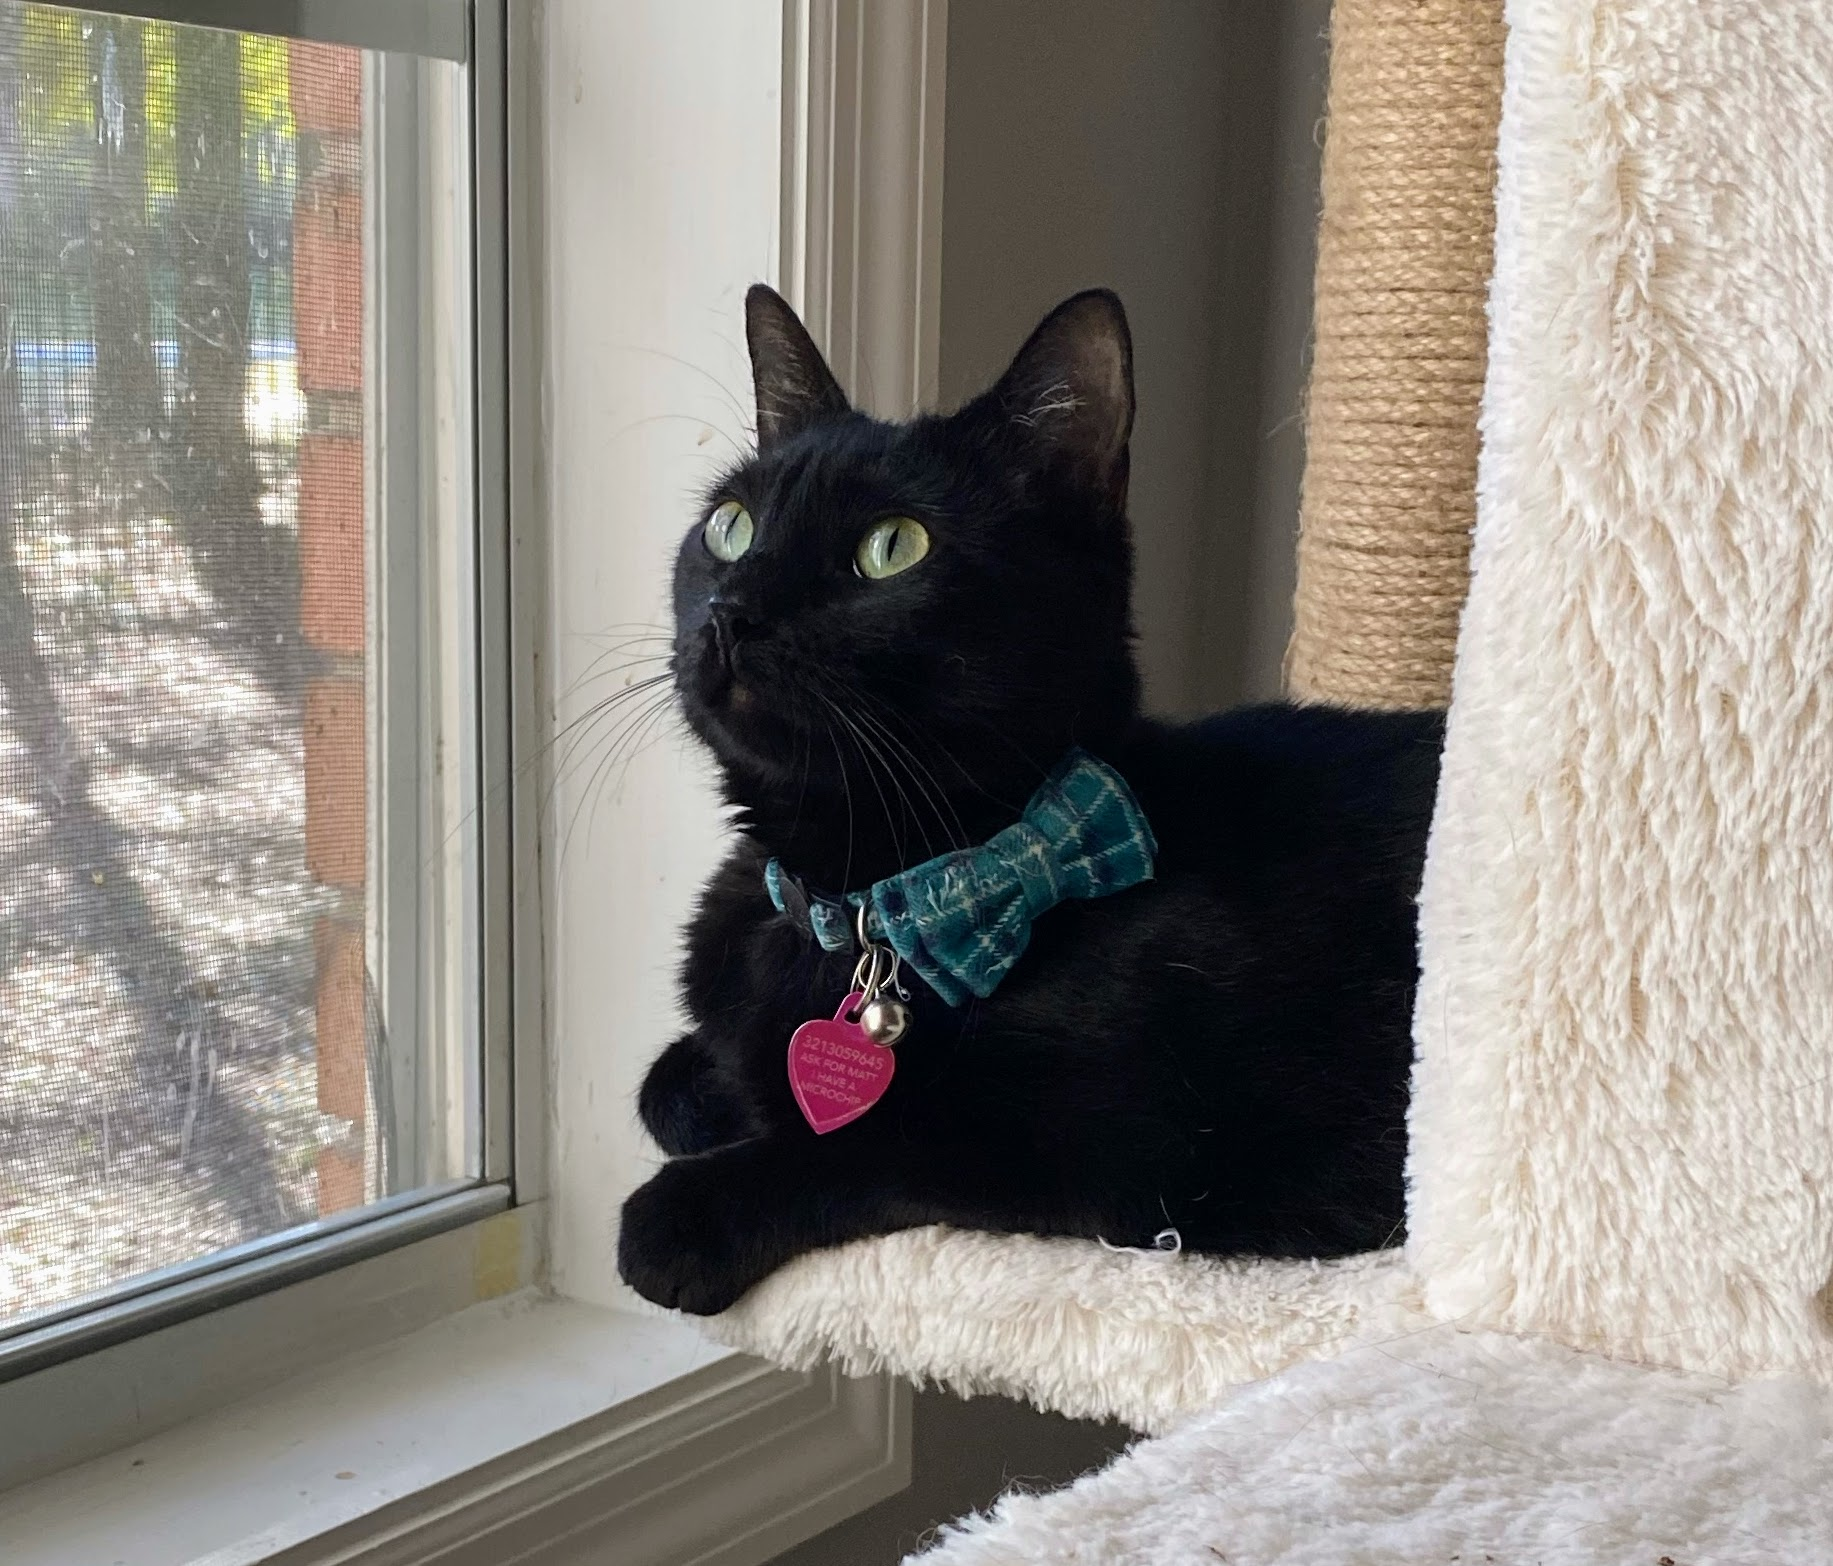
\includegraphics[scale=0.2]{bean.jpeg}
\end{center}

\tableofcontents

 \listoffigures
 \listoftables

\chapter{Abstract}

% The ``abstract'' is required and is limited to 350 words. % this version 344 words.

Augmented instruments have been around in some form for almost as long as instruments, but have had a relatively recent explosion in presence and capabilities due to the progression of technology through the 20th and 21st centuries. One potential use of augmented instruments is to control audio processing on a computer utilizing Max or other software environments. By being able to control the music natural expressive means, the performer and composer are able to experiment with a variety of ways to make sound. A performer is able to hear their sounds and adjust their playing in order to change them in real time, or the sounds are able to react to a performer's movements automatically. creation of future music. One new instrument that works to combine these two ideas is the Cyberinet.

The goal of this project is to provide a method of computer-enhanced performance to the solo clarinetist with minimal interference to their normal performance practice. A performer utilizing the Cyberinet is able to seamlessly switch between a traditional performance setting and an augmented one. Towards this, the Cyberinet is a hardware replacement for a portion of a clarinet containing a variety of sensors embedded within the unit. These sensors collect various real time data gyroscopic data of the performer and air flow within the instrument. Additional sensors can be connected to the Cyberinet to further expand its capabilities, which allows for the unit to become customizable based on various performance needs. This data is then transferred to a computer via Bluetooth connectivity in order to use the data in any number of potential electroacoustic performance settings. 

In order to explore these new relationships, in addition to the instrument itself, a collection of Max objects designed from the ground up to utilize the Cyberinet’s data in musical contexts has been developed. These Max objects were utilized in the performance of four new compositions for the Cyberinet in the spring of 2023.

\mainmatter
\chapter{Defining the Cyberinet}

The idea of augmenting an instrument has been around for almost as long as instruments themselves. In the modern sense, an augmented instrument can be defined as any acoustic instrument that has had an increase in functionality due to additional, usually electronic, additions to the instrument\cite{miranda_Wanderley_instrumentControl_2006}. While descriptive, this definition leave room for interpretation in exactly how or why the instrument is augmented. This leads to a large variety in terms of potential augmentations; some of which will be naturally more accessible and adaptable than others. Some of the more common less-desirable traits present in augmented instruments include: requiring permanent alterations to the performer's instrument\footnote{If removable, the setup process is cumbersome or time consuming}, high price, and the act or performing with the augmentation proves difficult to learn, or highly contrasting to the performer's training. 

The Cyberinet is a new augmented instrument indented to address all of these concerns by easily allowing a clarinettist to not only control audio/visual processing within the Max environment, but is also adaptable with a variety of sensors in order to create a custom setup unique to each user and performance setting.

To qualify as an augmented instrument and not a derivative new instrument, it is important that the augmented instrument retain enough of the original characteristics of the acoustic base\cite{miranda_Wanderley_instrumentControl_2006}. For example, an electric guitar can still functions as a guitar when not utilizing the amplification, or that a trombone still acts like a trombone regardless of when a mute is inserted. Without the context of a base instrument, an augmented instrument is no longer augmented, simply a new instrument. In order to address this concern, the Cyberinet functions as a digital enhancement to the Clarinet. The barrel of the horn is replaced with the Cyberinet unit, which collects a variety of positional and airflow data for use in digital processing without impeding the traditional performance practice of the instrument.

\begin{figure}
    \centering
    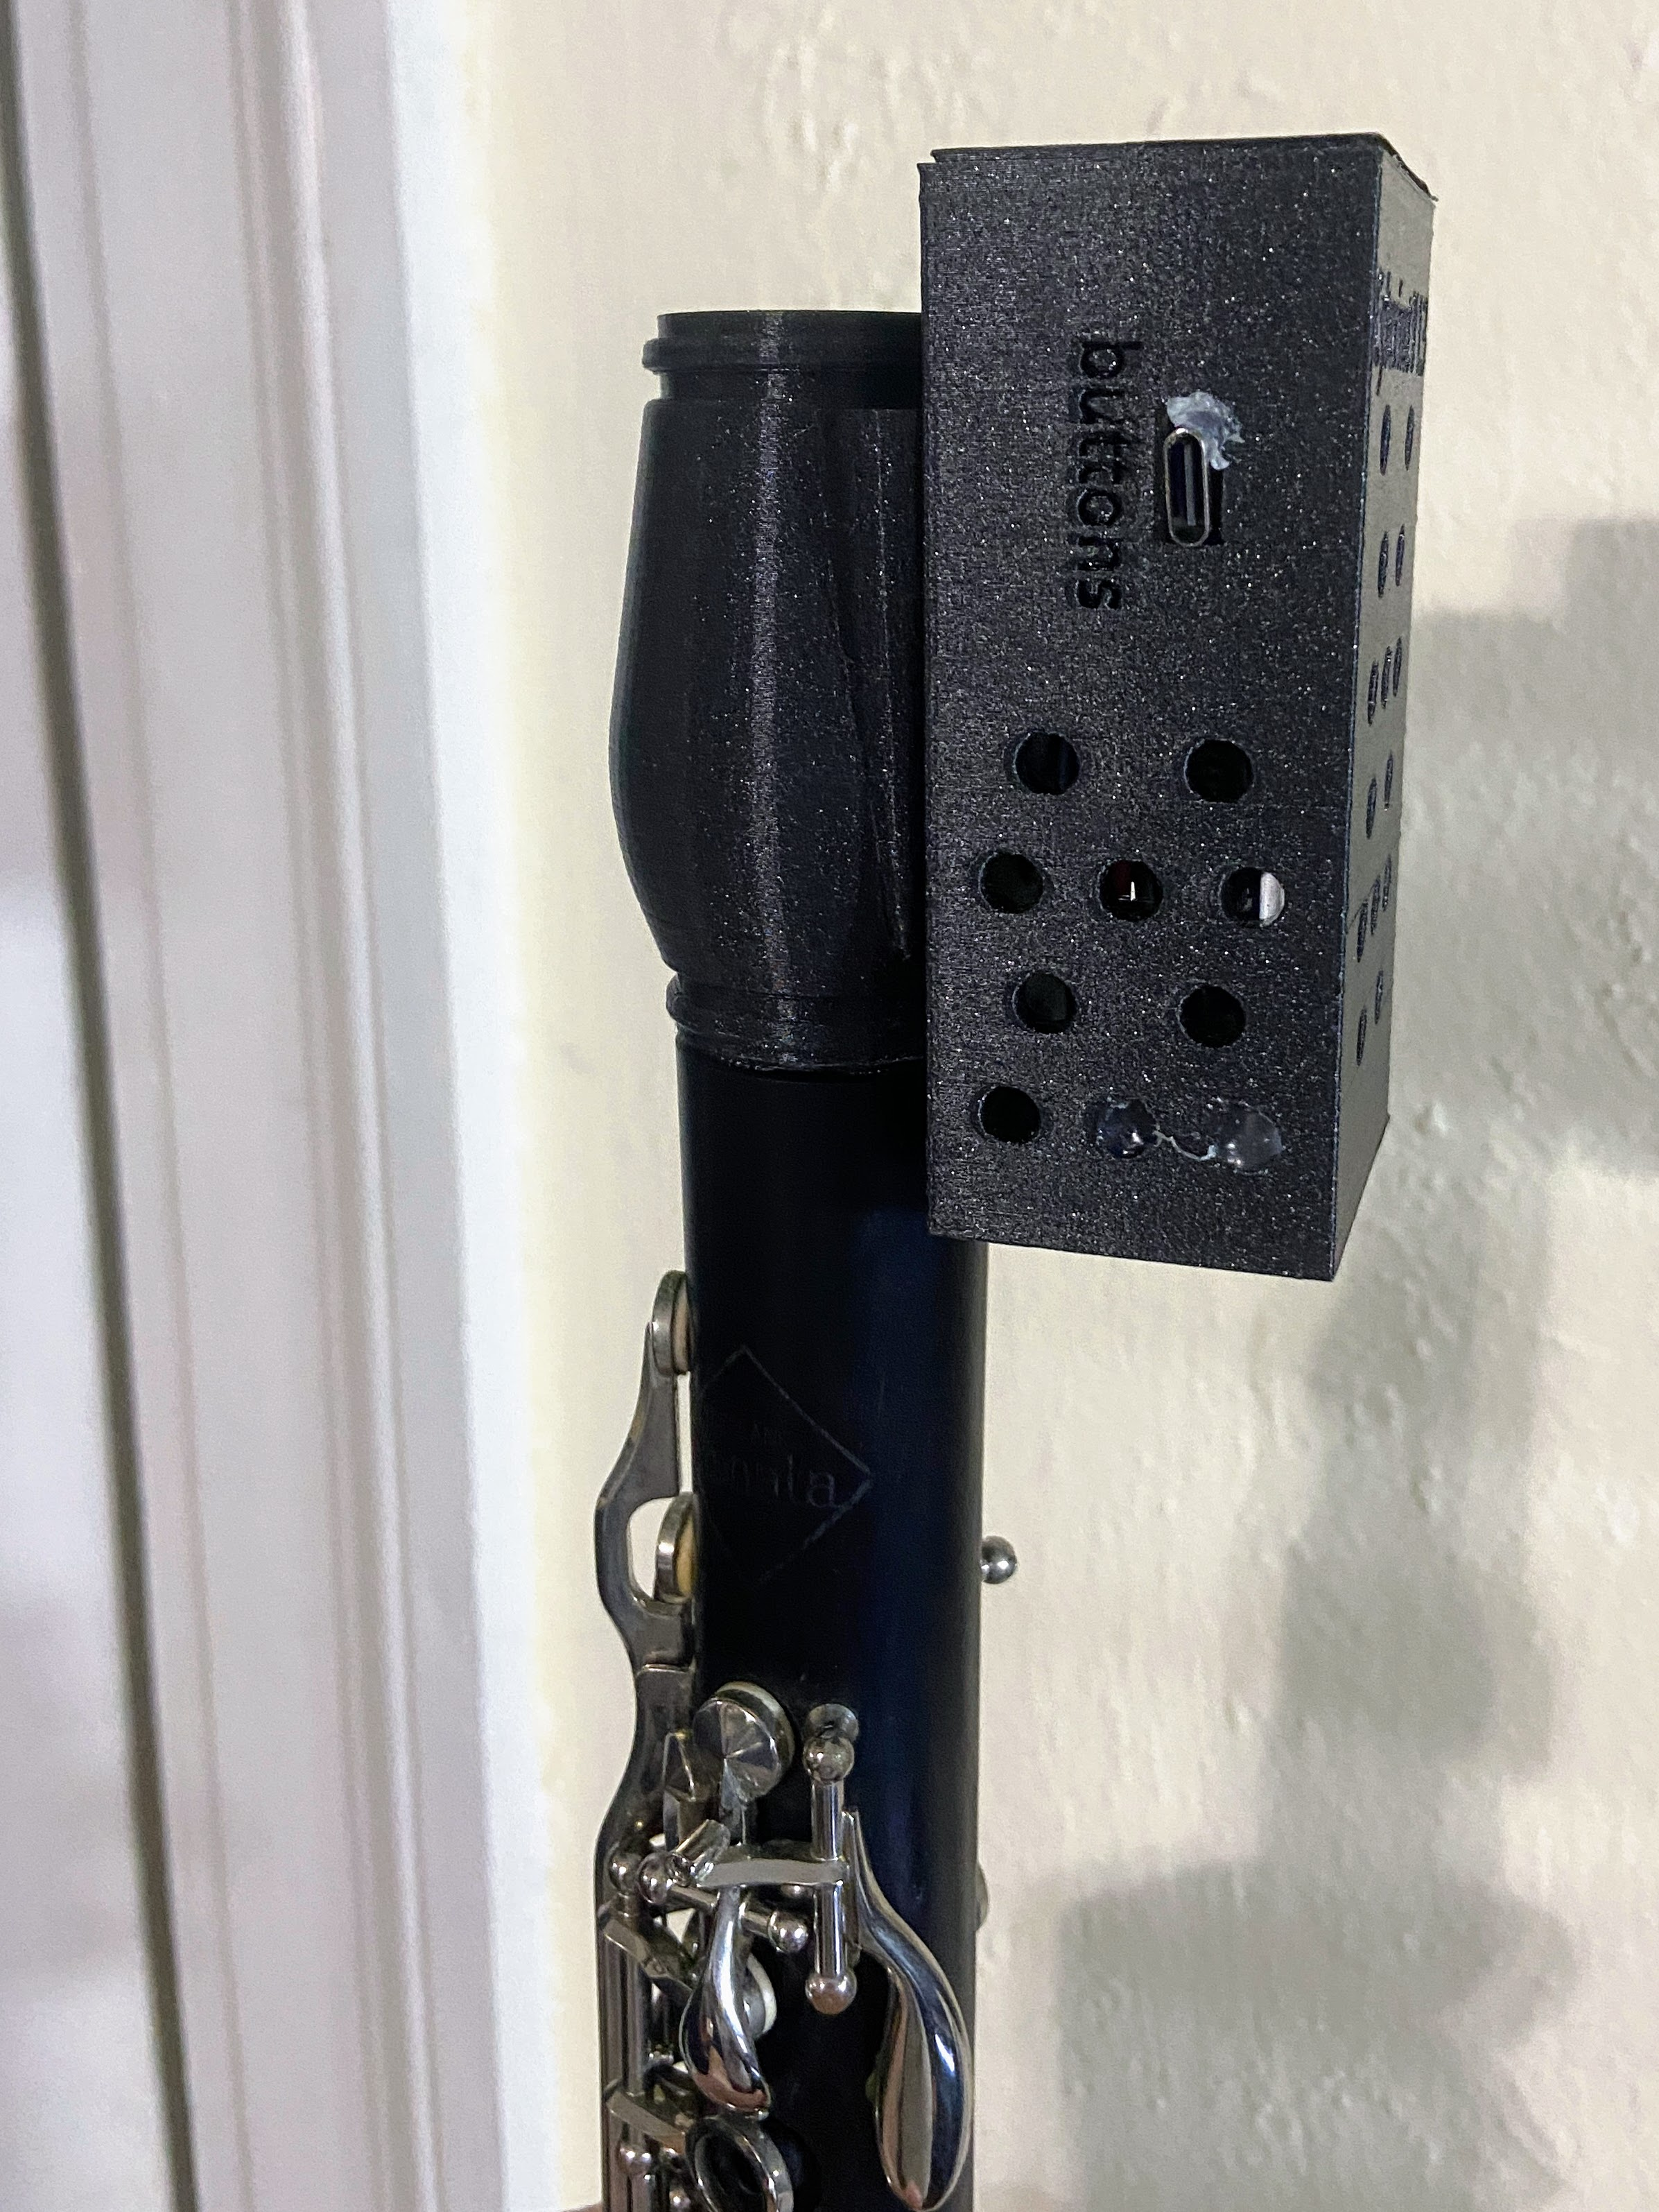
\includegraphics[scale=0.1]{diagrams/IMG_2212.JPG}
    \caption{Cyberinet main unit on a clarinet. (without mouthpiece)}
    \label{fig:my_label}
\end{figure}

This data is collected through multiple I2C sensors and wirelessly transmitted to a computer in order to control digital signal processing using the Max software. This allow for the performer to respond to the state of the processing by changing how they are performing in real time. The Cyberinet can be used to passively collect data for analysis, or with active use of gestures in order to achieve specific a sound or effect.

By being easily removable, non-invasive, and utilizing wireless communications, the Cyberinet addresses many of the concerns with augmented instruments. In terms of cost, the Cyberinet is completely open-source and costs approximately \$100 USD to produce\footnote{This value is the total cost of all sensors, PCB's, and other materials. The cost of a 3D printer is not included in this total.}. This, combined with a free collection of Max objects designed to interface with the Cyberinet's sensors all for a larger number of people to easily implement the augmentation and create sounds.

\section{Augmented Instruments \& Music}

% define an augmented instrument, give at least two examples. Indicate what is good and what could be improved.

Above anything else, the Cyberinet is an augmented instrument. To better understand exactly what this constitutes, and explore the Cyberinet's augmentations, a better understanding of these inventions are required. Going back several hundred years until the early 21st century, completely mechanical, electronic, and digital augmentations have all been utilized in musical performance. While mechanical and electric augmentations are still commonplace in the 21st century, a majority of modern instrument augmentations are digital in nature.

\subsection{Mechanical Augmentations}

\subsubsection{Brass Mutes}
In many contexts, the idea of augmenting instruments is viewed as a relatively new practice. While there has been an increase in the number of augmented instruments, especially those with electronic and digital augmentations, over the past century, the concept of improving the capabilities of instruments proceeds the electrical manipulations by centuries. These augmentations usually involve the addition or refinement of the physical attributes of the instrument.

To clarify this viewpoint, four historical examples will be discussed. The first is the development of brass mutes. By itself, a brass mute serves as an entirely mechanical and removable augmentation for the instrument it was designed for. A brass player utilizing a mute has a greater range of timbral options when compared to a performer not utilizing a mute. While not the first known instance of a mute being used in modern music, the score to Montiverdi's 1509 opera \textit{Orfeo} opens with this distinct timbre in the trombones, and is well known in Western music history.

\begin{figure}
    \centering
    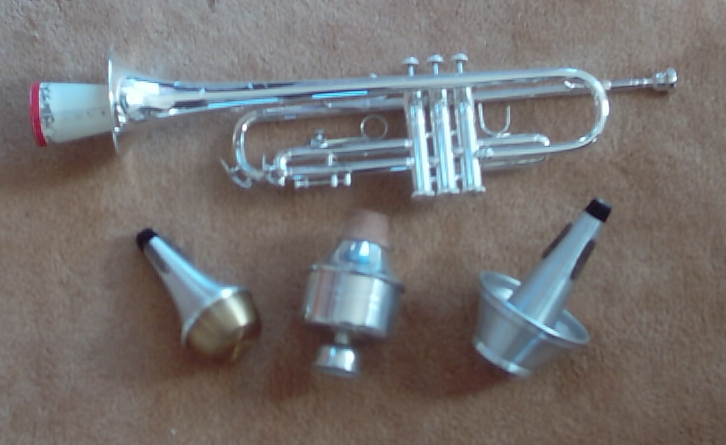
\includegraphics[scale=0.35]{diagrams/TrumpetMutes.jpg}
    \caption{A variety of trumpet mutes, courtesy of Wikimedia Commons.} %wikimedia commons. No permissions needed to use.
    \label{fig:tptmutes}
\end{figure}

Modern versions of brass mutes have been made for every common-place brass instrument\footnote{By common-place I am referring to those used in Western orchestras and bands. These include trumpets, horns, euphoniums, trombones, and tubas.}, and many varieties of mutes have been created to allow for a greater variety of timbre possibilities in both performance and orchestration settings. While different mutes will vary slightly based on the instrument and type, they all generally work by achieving one goal: absorbing/shifting a portion of the instrument's produced sound waves, filtering the sound, and changing the timbre. Some mutes such as cup and bucket mutes serve to block the sound waves in the air. Harmon mutes create a resonating cone to change the harmonic make up of the sound. Practice mutes serve to minimize the vibration of the bell before the energy can be converted into sound waves. The physicality of the mutes will also block a portion of the air moving through the instrument which both alters how the performer must play their instrument, as well as further altering the sound\cite{brassMutes1982}.

The specific acoustic properties of each brass mute are outside the scope of this document. However, the ability for a user to easily implement changes to their sound by altering the instrument in some way, thus augmenting their timberal range, is the core concept that makes a brass mute fit into the realm of augmented instruments.

\subsubsection{Prepared Piano}

Following a similar logic as brass mutes, a prepared piano can be viewed as an augmentation for a traditional piano. The creation of the prepared piano is attributed to John Cage in his 1938-40 composition \textit{Bacchanale}. While more complex and involved than a brass mute, the same concepts apply to the prepared piano. A performer is able to augment the timbral capabilities of the original instrument, the augmentation can be reversed, and the instrument still retains its identity as a piano while prepared. Because of how long it takes to properly augment a piano however, it is less flexible in a performance setting than other augmented instruments. 

\begin{figure}
    \centering
    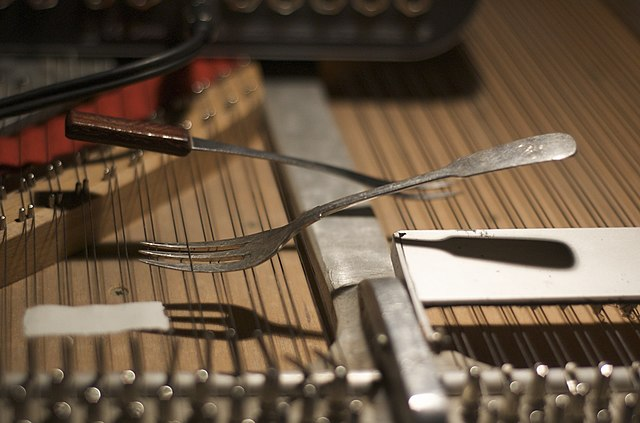
\includegraphics[scale=0.5]{diagrams/Prepared_piano_board_Neumann.jpg}
    \caption{An example of a prepared piano, courtesy of Wikimedia Commons.} % wmC. no attribution neededr
    \label{fig:pp}
\end{figure}

The process of preparing a piano is a relatively simple one, although usually time consuming\cite{ppVideo}. The most common of preparations involve placing small objects of varying materials wedged in between the strings for certain notes. Many composers will include a legend indication how to properly prepare the piano in the materials for a performance. These instructions usually include the specific strings, the item/material to utilize, and where/how to place it along the length of the string. Table \ref{fig:siPrep} recreates a portion of preparation instructions made by John Cage for his work \textit{Sonatas and Interludes} (1946-48). In the case of Cage, he provides specific locations as to where each material should be placed and which strings it should be threaded through. however he is more generic in his material description, allowing for interpretation\cite{ppVideo}. 

\begin{table}[]
    \centering
    \begin{tabular}{|c||c|c|c|}
    \hline
        Tone   & Material & Strings & Dist. \\
        \hline
         D4 & plastic & 1/2/3 (over 1, under 2-3 & 4 1/8 in \\
                  & rubber & 1/2/3 & 9 3/4 in \\
                  \hline
         D-flat 5 & rubber & 1/2/3 & 3 5/8 in \\   
         \hline
         C7 & furniture bolt & 2/3 & 2 3/16 in \\
         \hline
    \end{tabular}
    \caption{ reproductions of preparation instructions for three notes from Cage's \textit{Sonatas and Interludes}}
    \label{fig:siPrep}
\end{table}

\subsubsection{Instrument Keys}

Moving forward a few centuries from \textit{Orfeo} (1509) sees the development of the clarinet. Beginning around 1700, the clarinet is an evolution of the chalumeau which greatly expanded the older instrument's range.\footnote{Because the Clarinet did not have a strong lower register like the chalumeau, it is considered a new instrument rather than an augmentation. It is the same logic that defines instruments like the basset horn and bass clarinet as separate instruments instead of an augmentation of the clarinet.} With the chalumeau originally only having two keys, in the decades following the clarinet's inception, many mechanical augmentations were developed for the instrument. These augmentations were largely the addition of and improvement to the keys and key mechanisms. A small slice of that development is shown in figure \ref{fig:clKeys}. 

The end result of centuries of development is the modern clarinet's current physical shape with 17 keys\footnote{The exact number of keys on a modern clarinet can vary from 17-19 depending on the specific make and model of clarinet.}, watertight seals, and changes in instrument material from the original iteration. Unlike brass mutes and the majority of instruments discussed in this chapter, the addition of keys to augment the instrument is a permanent augmentation. 

\begin{figure}
    \centering
    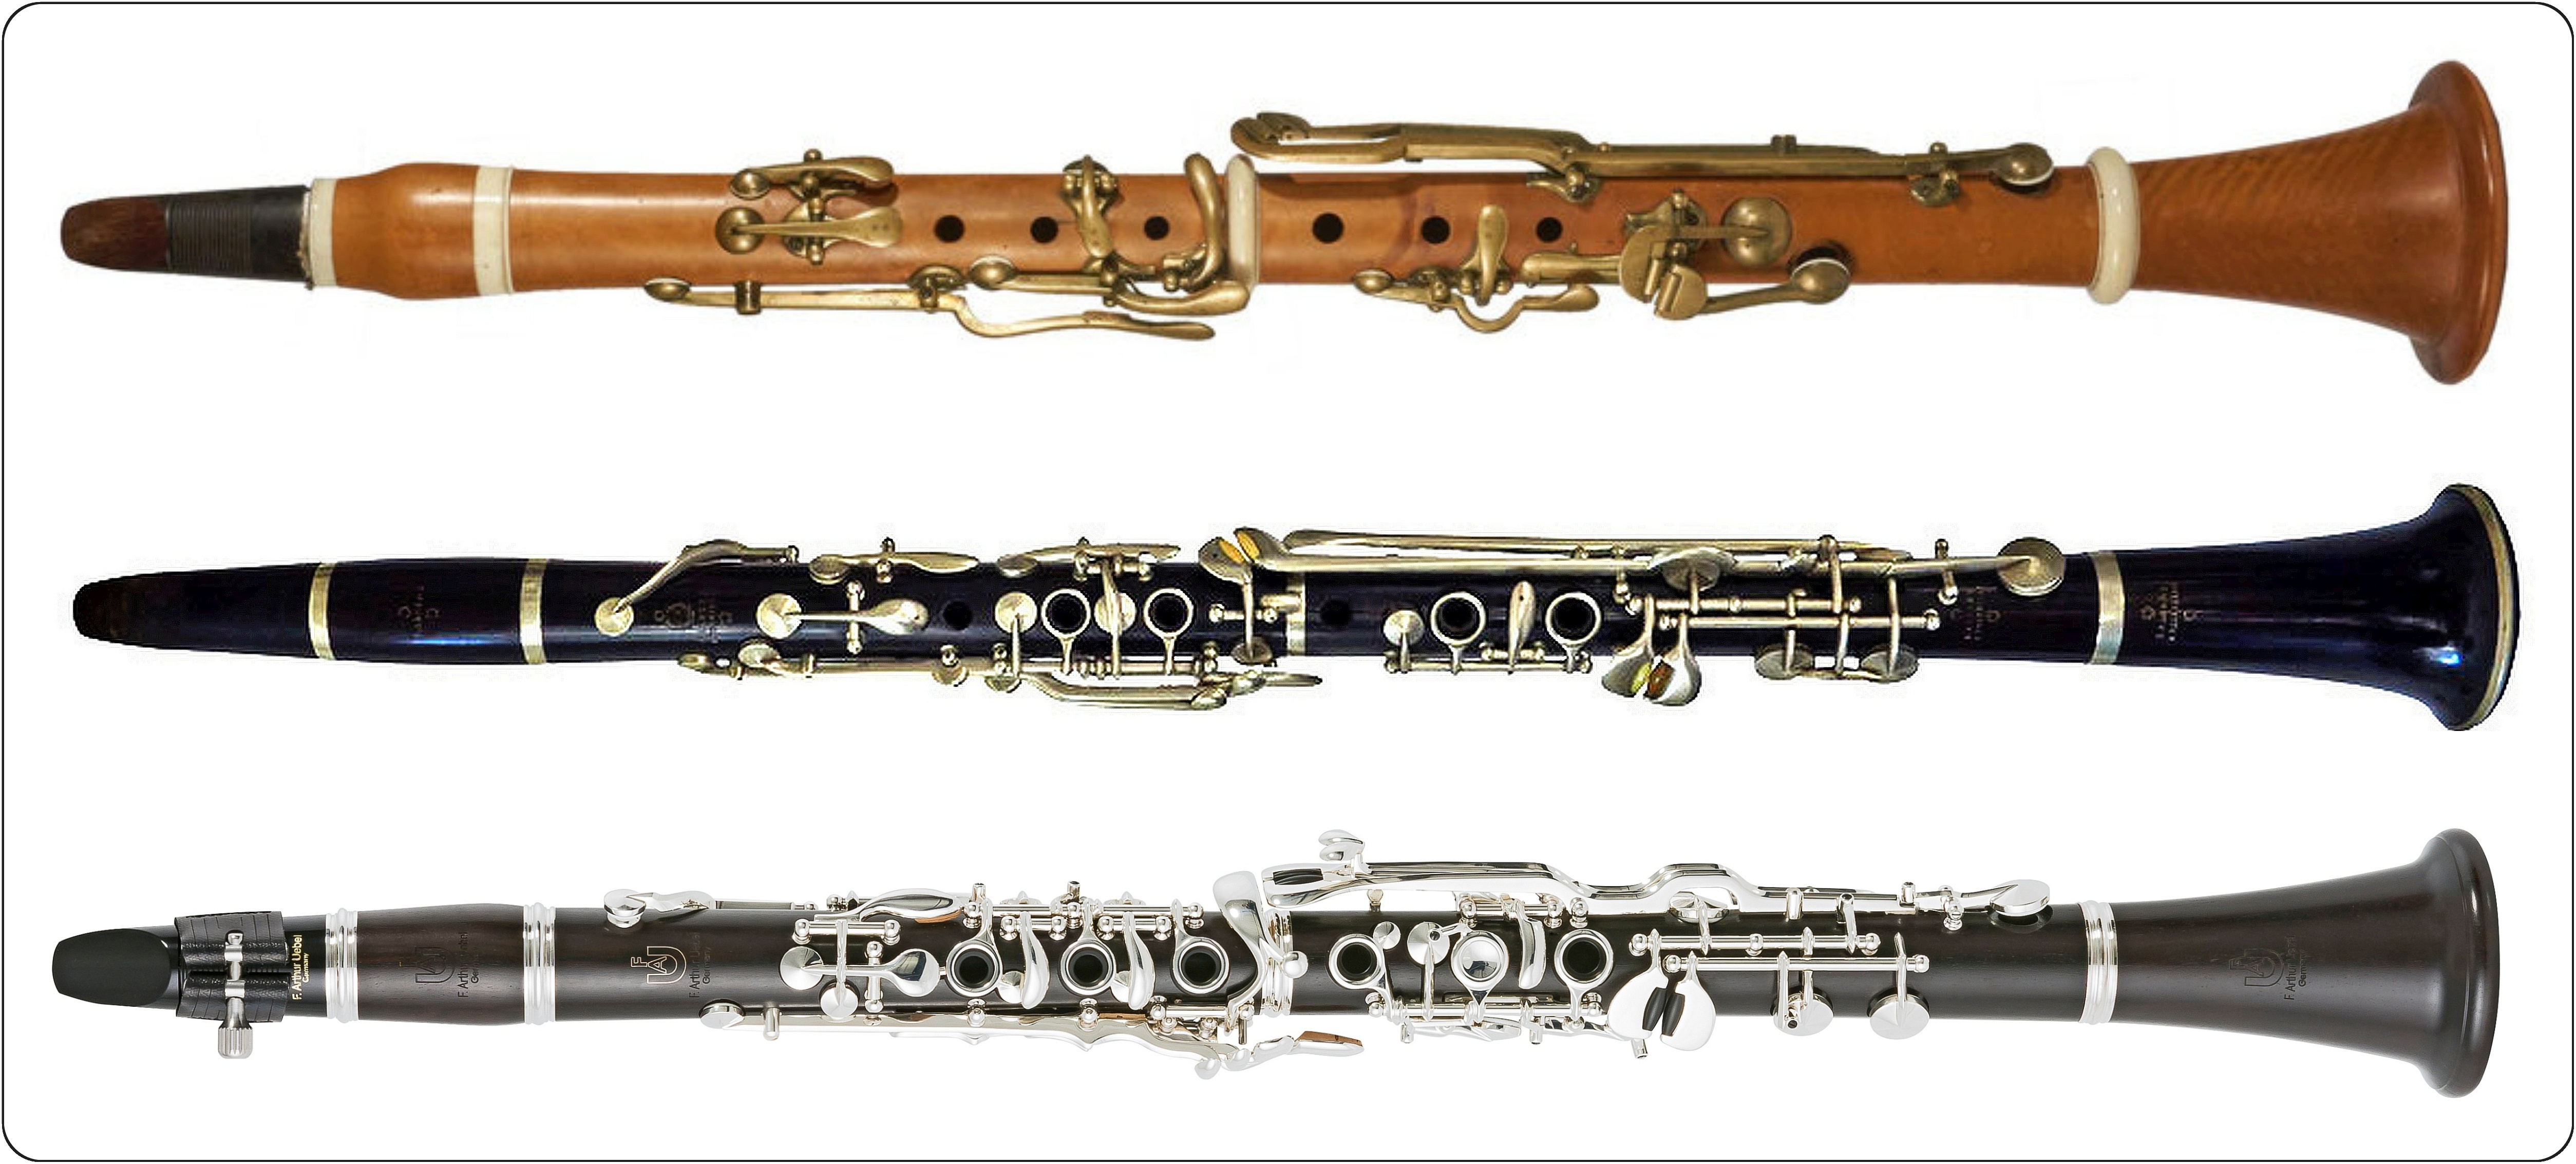
\includegraphics[scale=0.07]{diagrams/M-A-O-clarinets.jpg}
    \caption{A selection of clarinets showing differing levels of key development, courtesy of Wikimedia Commons.}
    \label{fig:clKeys} % wikimedia commons. no permissions needed. share alike
\end{figure}


\subsubsection{Player Piano}

The final augmentation discussed in this section came into development right at the end of the 19th century: the player piano. The player piano is a wonderful example of the idea of taking an acoustic instrument and enhancing its natural capabilities through additional mechanical or electronic components. Similar to the addition of keys to the clarinet, but this augmentation was not spread over multiple centuries. This idea of augmented instruments began to grow as the components and technology capabilities increased in power while decreasing in price, and this technological trend starts, like so many others, shortly after the commercial harnessing of electricity.

\begin{figure}
    \centering
    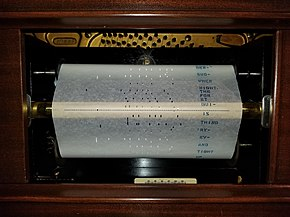
\includegraphics[scale=0.8]{diagrams/PlayerPianoRoll.jpg}
    \caption{A player piano roll, courtesy of Wikimedia Commons.}
    \label{fig:pianoroll} % not attribution, share aliske
\end{figure}

The player piano functions primarily as a traditional piano. There are no alterations made to the timbre or the action of playing the instrument. However, additional features have been added to the player piano compared to a completely acoustic one. Player pianos started out being controlled through the use of a large spool of paper, called a roll. Holes punched into this paper would be used to manually trigger levers to actuate the piano's hammer mechanisms and generate sound. Early versions of these instruments were operated with a manual pneumatic pump, operated with the feet. Throughout the 20th century, improvements were made to this mechanism including its electrification and eventual digitization. However despite the various technological improvements, a large portion of the market of player pianos is for historic and restored instruments.

The augmentation comes into play when compared to non-player pianos. A completely acoustic piano will not make any sound unless acted upon, and then each note must be played in real time to create music. Player pianos are able to perform previously notated music. As the music of Colon Nancarrow (1912-1997) shows, this playback can be significantly more complex than what is possible through human means. Largely know for his work with player pianos, Nancarrow experimented with complex, multi-dimensional canons and tempo relationships between different voices. The end result of which are works for piano that are physically impossible for a traditional performer to reproduce. By utilizing the player piano, Nancarrow was able to embrace this aspect of his music, rather than changing it to match what was traditionally possible.

By being able to play back music, player pianos allowed for a greater spread of music when audio recording was still in its infancy\footnote{I personally like to view the player piano as analogous to MIDI or similar to MP3 playback of the 1890s}. The instrument's use of permanent, yet optional augmentations is similar in nature to that of the electric guitar.



\subsection{ Analog \& Digital Augmentations}
The difference between 20th and 21st century augmented instruments is ambiguous at best. Electrical augmentation is still prevalent in the practice, but as the components become smaller and more affordable, a further increase in the number of instruments can be seen\footnote{Simply scrolling through the archived NIME and ICMC conference  proceedings will this growth in the number of papers related to augmented instruments.}. Because digital augmentations are by nature electronic, designating them as analog or digital would prove a better taxonomy than electric vs digital, or 20th century vs 21st. However, determining the most ideal designation of varying augmented instruments is outside the scope of this discussion. As computers increased in power, their usage to both locally and remotely to control augmentation has also increased.

\subsubsection{Electric Guitars Pickups}

During the 20th century is when a large number of augmented instruments begin to be developed. This is due in no small part to the development and commercialization of audio amplification and recording during the late 19th and early 20th centuries, as well as improvements to those technologies throughout the century. One example of an electronically augmented instrument is the Electric Guitar, which was developed in the 1930's by adding electronic pickups to acoustic guitars\cite{electric_guit_history}. The addition of a pickup is one of the more simple-yet-effective augmentations that can be done to an instrument. The analog signal can be recorded, amplified, or altered with circuitry for a variety of uses both in recording and performing live music. In fact, this is the basic for guitar effect pedals. In short, why a pickup is so effective is that it is a simple sensor that can be applied to a large variety of processes; a feature shared with the Cyberinet and many other instruments.

\begin{figure}
    \centering
    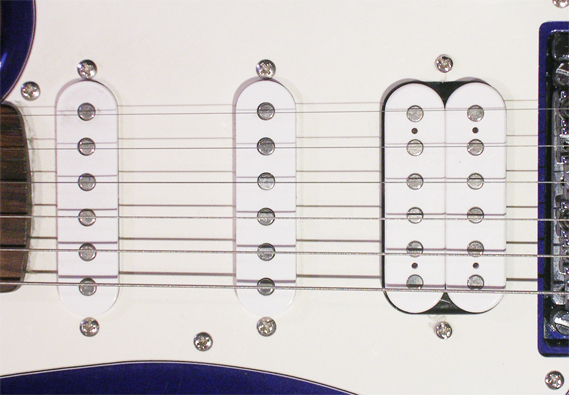
\includegraphics[scale=0.5]{diagrams/Pickup-SSH.jpg}
    \caption{Guitar pickups showing magnets underneath each string. Courtesy of Wikimedia Commons.} %public domain image
    \label{fig:pickups}
\end{figure}

Guitar pickups function similarly to dynamic microphones and speaker cones. Each pickup contains a magnet wrapped in a metallic coil placed underneath each string of the guitar. When the metallic strings vibrate, the vibrations cause fluctuations in the magnetic field, resulting in analogous electrical signal to be generated and sent to be altered or amplified\cite{coils09}.

\subsubsection{MIGSI}

The Minimally Invasive Gesture Sensing Interface, or MIGSI, Trumpet is an augmented instrument designed to work with the ergonomics and performance practice of the traditional trumpet\cite{reid2016}. Towards this goal, creator Sarah Belle Reid developed a collection of sensors that fit seamlessly into the form factor of the trumpet. These sensors work to capture control data such as valve placement, hand tension, instrument position, etc. and send it wirelessly to a computer. Infrared sensors are utilized to measure the vale position when fingering various notes, Force-Sensing resistors (FSR's) to measure the placement and tension within the hand holding the instrument, and accelerometers to measure instrument movement. While the sensors that make up MIGSI are removable, all of the images of the instrument, such as figure \ref{fig:MIGSI}, show that these are held on with bolts, which is not conducive to a quick swap if a performer needed to suddenly remove the augmentation.

MIGSI collects data and transmits to a computer to be utilized in some process. To help with this process, MIGSI is compatible with Max and other programs which can receive serial data\cite{reid2016}. Reid et. al have developed a platform which receives Open Sound Control (OSC) data for a wider range of software compatibility.\cite{reid_2019}. In order to demonstrate the effectiveness of the instrument, Reid has created several improvisations and compositions utilizing MIGSI, such as \textit{Consider} (2017) and \textit{Pocket Fig} (2015).

\begin{figure}
    \centering
    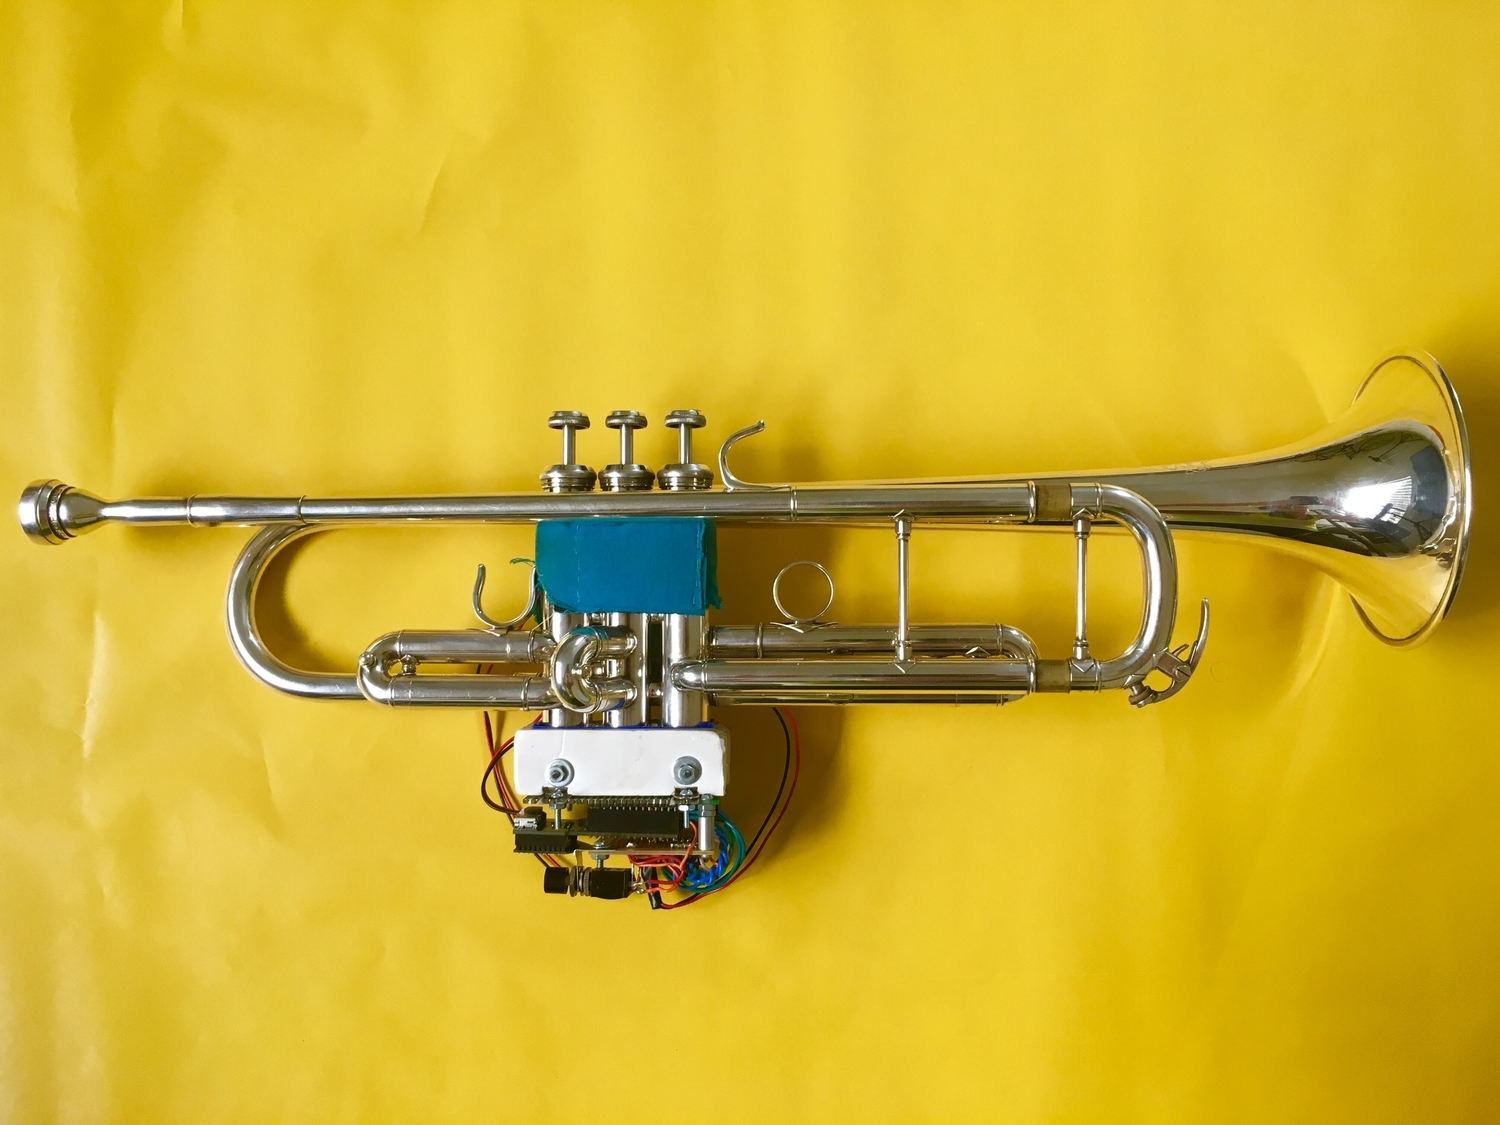
\includegraphics[scale=0.25]{diagrams/MIGSI.jpg}
    \caption{Photo of the MIGSI trumpet, used by permission.}
    \label{fig:MIGSI} % from sarahbellereid.com/migsi
\end{figure}


Here we will discuss \textit{Pocket Fig} for the MIGSI Trumpet, written by Sarah Belle Reid\footnote{A performance video of \textit{Pocket Fig} can be found at \url{https://www.youtube.com/watch?v=5szWkbVjYxg}}. In this semi-improvisatory work, Reid utilizes the FRS's as well as Infrared sensors to collect data related to the position and valve displacement on the instrument\cite{reid_2019}. This data is then wirelessly sent to the computer to control a Max patch's granular synthesis processing. The end result is, in Reid's own words from the online performance description: 

\begin{quote}
    "a flurry of classic computer music sounds, stutters, and granular synthesis gestures based on the voice and trumpet sounds of the performer."
\end{quote}

This flurry of effects are heard in performances as soon as the performer releases a trumpet valve. this gesture triggers a randomized playback of multiple grains taken from the recording of the performance. As the work continues, additional latency between the gesture and effect are intentionally introduced in order to subvert the viewer's expectations and allow for more interplay between the sounds and the performer\cite{reid_2019}.


\subsubsection{SABRe}

The SABRe is another sensor array, but this one is designed to work with the clarinet, but is also compatible with various other single-reed woodwinds, opposed to the trumpet. The unit straps onto the instrument and can be used to collect airflow and position data to be wirelessly sent to a control computer. While effective and easily removable, this particular device offers a relatively limited amount of usable parameters which can be utilized in an augmented instrument. In the majority of cases this is not problematic, as like the MIGSI, the choice in sensors matches with the common performance gestures of the instruments using it\footnote{We will see modularity in physical design come into play with the Cyberinet.}. 

Similar to MIGSI, SABRe is intended to also be minimally invasive to the performer. It is intended for use mainly with clarinets, being originally prototyped on a bass clarinet, but can be easily applied to almost any single-reed instruments\cite{Schiesser2012}. The goal of the SABRe is to provide augmentation features to performers, regardless of their technical abilities\cite{Schiesser2012}. To help with this, SABRe comes with a variety of bands to attach the main unit to different sized instruments. 

SABRe utilizes four main sensors as well as an additional set of buttons that can wirelessly communicate with the main unit. These include gyroscopic and accelerometer data, airflow sensors, and buttons.\footnote{There are a few more sensors in the SABRe, but the ones mentioned are the main ones advertised.}

\begin{figure}
    \centering
    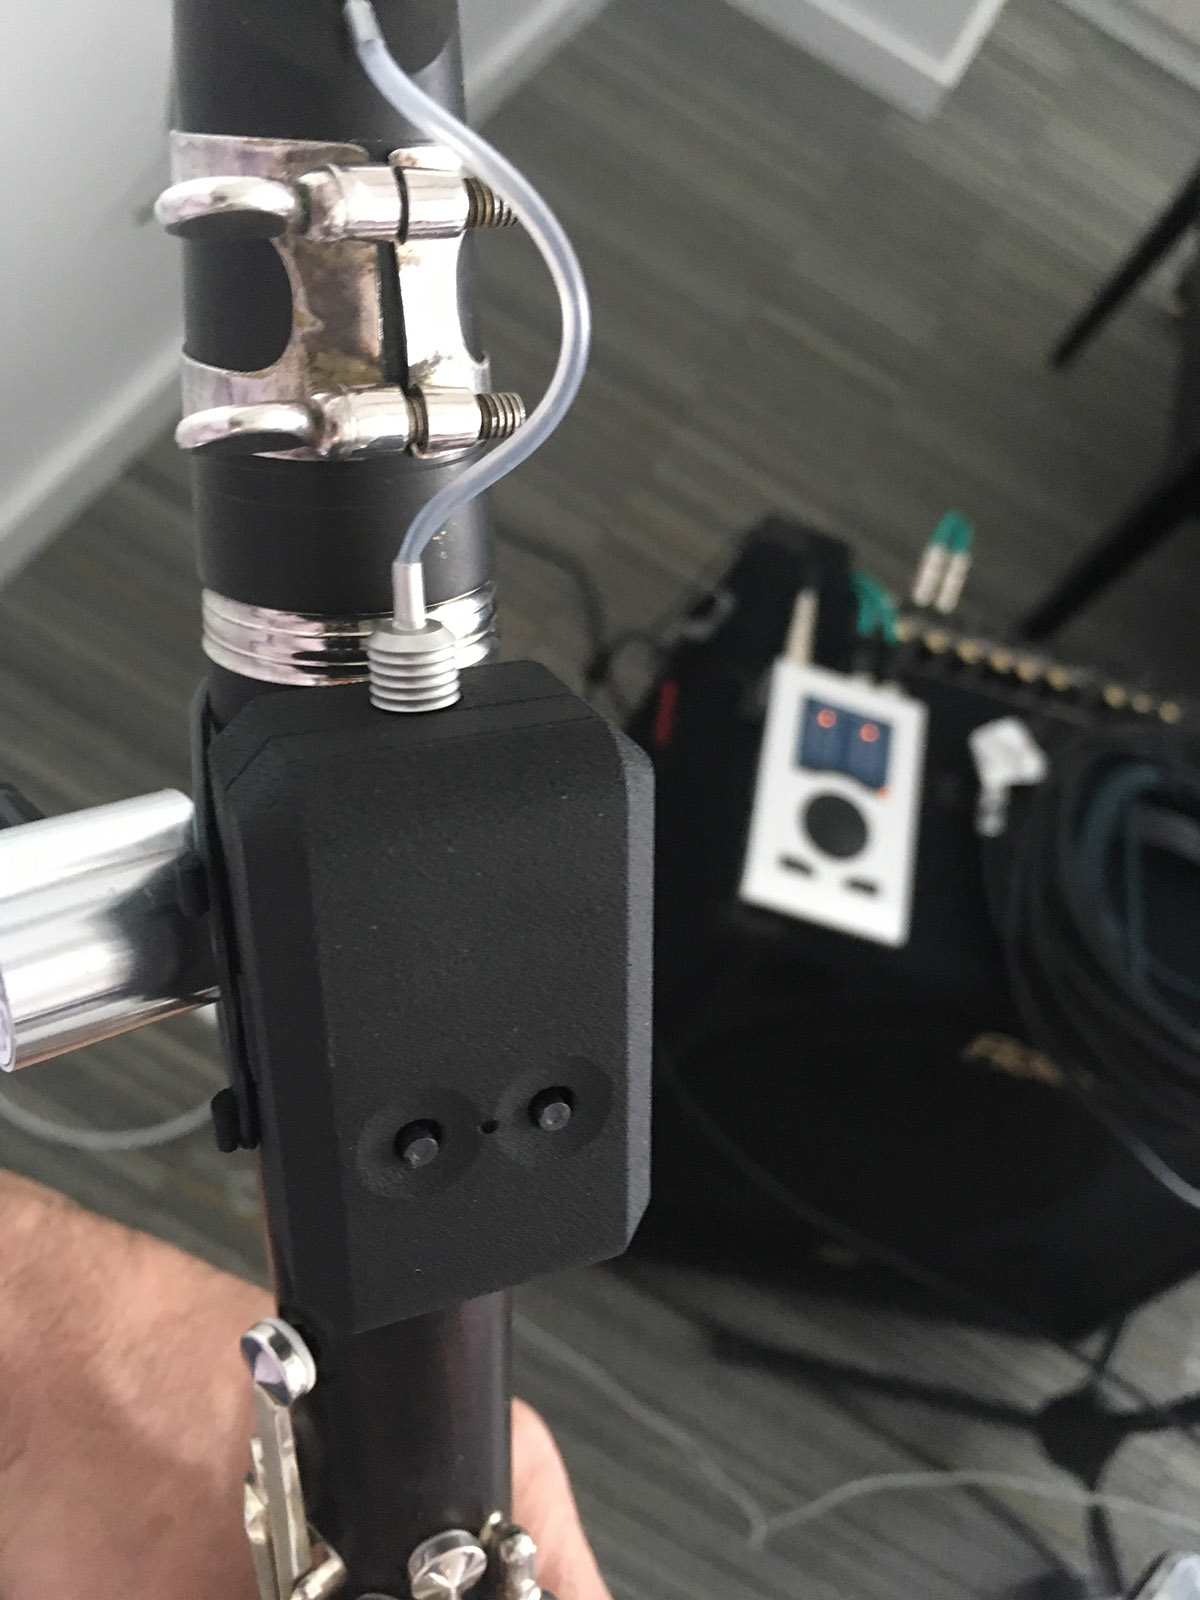
\includegraphics[scale=0.2]{diagrams/sabre-right-hand.jpg}
    \caption{SABRe on a clarinet, from \url{https://www.jeanfrancoischarles.com/2018/11/first-look-at-sabre-clarinet-sensor.html}}
    \label{fig:SABRe} % from a blog, no contact information on website.
\end{figure}


SABRe contains a similar base to the Cyberinet in terms of sensors. The main sensors included in the SABRe are a gyroscope and accelerometer which can monitor the performer's movement in real time. There is also an airflow sensor which can detect the air leaving the performer's mouth as it passes the mouthpiece. This is done with a special order mouthpiece pad containing a notch for the sensor tube to rest in. While ingenious in terms of placement, if the pad wears out and the performer is unable to receive a new one from SABRe, then that sensor becomes useless until the pad is replaced since that is all that is holding the airflow tube in position. There are additional sensors as well such as a thermometer, but these are not utilized as much in performance as the aforementioned sensors. Both SABRe and the Cyberinet also have a removable set of buttons that can be triggered as needed by the performer.


Prior to early 2023, SABRe had been on a hiatus in terms of development and is currently in the process of designing a relaunch of the system. It is perhaps for this reason that there is a limited number of works for and writings about the system, but discussing the reasons behind the hiatus is beyond the scope of this paper. Unfortunately however, the majority of resources provided by SABRe online have been taken down and not publicly backed up pending their eventual relaunch of the system. Differences may occur between the original version, discussed here, and the eventual second iteration. The original design utilized a software program developed by SABRe to control the receiving and control of the data for audio processing. 


One piece that will be discussed is \textit{Sailing}\footnote{The performance of \textit{Sailing} can be found at \url{https://www.youtube.com/watch?v=Eiuacb5nJc8}} by the SABRe's creator: Matthias Mueller. In this work, Mueller takes the gyroscopic information from the SABRe to control audio effects in real time. The first one heard is the control of the amount reverb and delay time as the performer moves from right to left. This is followed by triggering a tremolo effect that combines with the clarinet timbre. Due to a lack of a score and other resources due to the aforementioned relaunch of the system, it is my best guess from the video that this effect is being toggled on with the buttons located on the back of the instrument. By combing these effects with micro-tonal notes, Mueller is able to create a unique sound world easily and effectively.

Mueller also utilizes a pitch shifting effect, but it is unclear to me if it is created as a unique harmonizing effect, or is created as a byproduct of adjusting delay times. The final effect is a little distortion present when the performer reaches the extreme ends of the accelerometer data range.

In the future, should a performance score or the software patch become available, it would warrant more in depth analysis of the performance practice and specific utilization of the SABRe's sensors. However, there is still much that can be learned with Mueller's performance video. It can be seen that Mueller clearly focusing on only a handful of sensors present within the SABRe: the accelerometer and buttons. By focusing on a smaller subset of the sensors, it allows Mueller to allow the capabilities to the system to stand out. It becomes very clear what the correlation between the clarinetist's physical position and the timbres being created are.

Mueller's utilization of the button is worth bringing up individually. In \textit{Sailing}, Mueller is using this button to trigger a tremolo-like effect to be applied to the clarinet's signal. Unfortunately without the software patch or score the fine details of this are left to speculation, but I want to focus on the idea of manually triggering an effect with a button. Unlike a foot pedal, these buttons follow the performer, allowing them to take full advantage of the buttons along with the movement sensors. A performer can access the buttons regardless of their on-stage location. The buttons can also be placed in various locations around the stage if needed, limited only by the length of a cable or the distance of the Bluetooth connection. Having a mixture of continuous and momentary sensors\footnote{The buttons are momentarily on when pressed, while the other sensors are continuously monitoring data values} allows for the performer to create instant (or near instant) changes in the software state like shown with Mueller's triggering of the tremolo effect. Both the Hyper-Flute and the Cyberinet utilize this mixture of momentary buttons with continuous sensors. The continuous sensors can be either digital or analog, that does not effect the relationship between them and the buttons.


\subsubsection{Hyper-Flute}

There are many more augmented instruments that have been developed in the 21st century so far. A full study of them would warrant an entire other dissertation\footnote{A few other examples include the Meta-Sax, Overtone Violin, Haptic Drums, the instruments discussed by Reid et. al\cite{reid2018}, and instruments developed by the Augmented Instruments Laboratory in London.}. Here, we will wrap up our discussion of digitally augmented instruments with the Hyper-Flute.

\begin{figure}
    \centering
    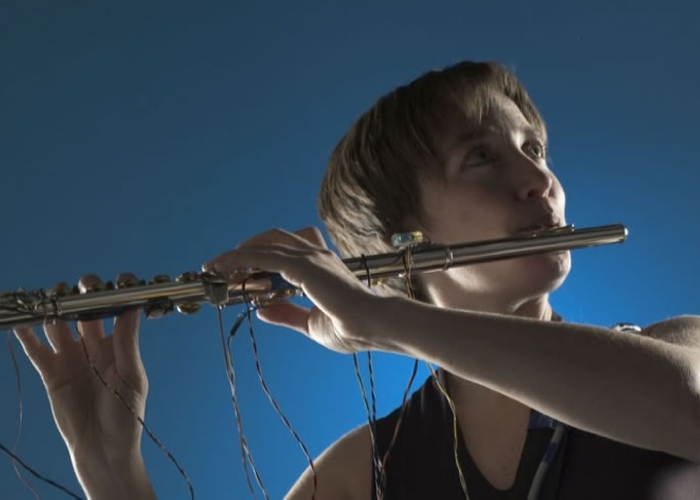
\includegraphics[scale=0.5]{diagrams/palacio_quintin_cleo.jpg}
    \caption{Cléo Palacio-Quintin performing on the Hyper-Flute, used by permission} % https://quasar4.com/en/repertoire/composers/cleo-palacio-quintin
    \label{fig:hyper-flute}
\end{figure}

Developed in 2003 by flutist/improviser/composer Cléo Palacio-Quintin, the Hyper-Flute is a Powell 2100 model flute with a handful of sensors embedded into various locations along the instrument. \cite{hyper-flute2003}. Palacio-Quintin's stated goals in developing the instrument are: 

\begin{quote}
    ...[to preserve] the intimate relationship between my body, my instrument and the sound it produces. I wanted to keep intact the acoustic richness of the flute, and my way of playing it. The computer had to become a virtual extension of the acoustic instrument \cite{hyper-flute2003}.
\end{quote}

Towards this goal, Palacio-Quintin ultimately decided on six unique sensors that can control the computer processing of the flute. While there are some overlaps between the Hyper-Flute and the other instruments discussed in this chapter, the design implements a variety of unique ideas not present in the other wind instrument augmentations discussed. Firstly is that the Hyper-Flute is not a removable augmentation like the Cyberinet, SABRe, or MIGSI. These sensors, listed in figure \ref{fig:hyper-flute-sensors} are permanently installed onto the flute. 


Voltages from each of these analog sensors are then analyzed and converted to a MIDI value which can be sent to a computer or MIDI compliant instrument. All of the data is sent as continuous control MIDI messages. What I find particularly interesting about the Hyper-Flute is that while Palacio-Quintin has developed various software patches using Max, similarly to the other instruments discussed in this chapter, because the data being generated is MIDI compliant, the Hyper-Flute can easily interface and control a large variety of instruments via the MIDI port, which can open an entirely different world of performance practice and possibilities when compared to other instruments\cite{hyper-flute2003}. Unique to the other instruments discussed throughout this chapter, the Hyper-Flute requires a separate interface in order to convert the voltages into MIDI data. Palacio-Quintin utilizes a Microlab interface for this purpose. This is a custom device created by A.J.van den Broek\cite{hyper-flute2003}. 

\begin{figure}
    \centering
    \begin{enumerate}
        \item Magnetic field sensors to detect pinkie-key movement.
        \item Ultrasonic distance sensor to detect distance from the computer.
        \item Tilt switches to detect movement and rotation of the instrument.
        \item Pressure sensors located where the performer holds the instrument.
        \item Light sensor to detect ambient lighting changes.
        \item Button switches which can be activated by the thumbs while performing.
    \end{enumerate}
    \caption{Sensors present in the Hyper-Flute.}
    \label{fig:hyper-flute-sensors}
\end{figure}

In musical performance, the use of sensors can be seen in \textit{Souffles Électriques}, a small collection of various works for the Hyper-Flute.\footnote{\textit{Souffles Électriques} can be found online at\url{https://vimeo.com/155153474}.} While not discussed in the original 2003 paper, Palacio-Quintin has since expanded the range of instruments to include at least the Bass Flute as well as the original Concert Flute. The performer is able to intuitively control the sounds from the various sensors. Effects such as adjusting audio processing and the playback of samples by pivoting the flute angles and position in three dimensions are seen in the performance, as well as the use of the magnetic field sensors in the pinkie keys.


\section{Cybernetics \& Music}
While not a design feature of every augmented instrument, many of ones discussed, especially those of a digital nature, allow for a level of Cybernetic interaction between the performer and the music. Much like electronically augmented instruments, Cybernetics is a relatively modern science with roots going back centuries. The core principals of which have brought about advancements in various fields such as mechanics, philosophy, health management, music, and more. 

\subsection{General Cybernetic Concepts} %% This needs a graphic of something in this subsection partway through.

The concept of modern cybernetics was defined by Norbert Wiener in his 1948 book \textit{Cybernetics: Or Control and Communication in the Animal and the Machine}, which has had its second edition republished by MIT press in 2019\cite{WeinerCybernetics2019}. The republished versions contain additional supplementary chapters not included in the original 1948 publication. In its original context, Cybernetics is defined by Wiener as: 

\begin{quote}
    "The science of communications and automatic control systems in both machines and living things."
\end{quote} 

While the concepts of Cybernetics were present before Wiener, it was in his writings that the term Cybernetic was formally created. The term is derived from the Greek kubernetes, which translates to the captain of a ship\cite{WeinerCybernetics2019}. Wiener credits J.C. Maxwell in his 1868 paper as one of the first formal studies into what would ultimately evolve into Cybernetics. In that paper, Maxwell discusses the concept of a Governor and Moderator within a variety of mechanical systems\cite{maxwellOnGoverners}. Wiener posits that perhaps one of the earliest examples of the work as described by Maxwell is that of the steering mechanism of a boat\cite{WeinerCybernetics2019}. Heavily summarized, this is the idea that a sailor can see and respond to the conditions they are sailing in by turning the wheel, which, through mechanical means described by Maxwell\footnote{Maxwell's original article is largely composed of complex mathematical operations based on hypothetical systems, and it beyond the scope of this paper.}, causes the boat to turn, thus altering its condition.

As time progressed, the definition of Cybernetics has evolved. Scientifically, the definition is relatively unchanged, still focusing on feedback systems and automated responses, but now is utilized in the development of artificial neural networks and machine learning\cite{Cariani2010}. In popular culture, Cybernetics often invoke ideas of half-organic/half-machine creatures. This connection is partly due to these creatures name, "Cyborg", which is a portmanteau of cybernetic and organism. The mechanical components are able to react to the state of the organic components and either enforce or act against what is happening in the body. A few examples of popular cyborgs are the Cybermen from \textit{Doctor Who}, the Borg from \textit{Star Trek}, RoboCop, Motoko Kusanagi from \textit{Ghost in the Shell}, and Numbers 17 and 18 from \textit{Dragon Ball Z}. All of these examples have utilized automated, mechanical components to augment some part of their body.

A real-world version of this are modern diabetes management systems such as the Omnipod 5 or Medtronic MiniMed. Looking specifically at the Omnipod\footnote{I actually haver personal experience utilizing the Omnipod 5 in order to accurately manage my Type One Diabetes. This was in no small part an inspiration for the ultimate direction of the Cyberinet.}, this insulin delivery device has the capability to be paired with a constant glucose monitor (CGM) embedded within the user's abdomen. CGM will read the glucose levels of the user and automatically adjust the Omnipod 5's insulin delivery rate to compensate for any changes to the blood glucose levels, and adapts its changes based on daily insulin dosages. This system is cybernetic in every sense of the word. It combines organic and inorganic components like in popular culture, as well as the internal feedback loops to control the blood glucose level of a diabetic in a manner similar to a person without diabetes, as in the scientific definition.

\begin{figure} % Need a graphic for this, but may have to make one since this is a major company
    \centering
    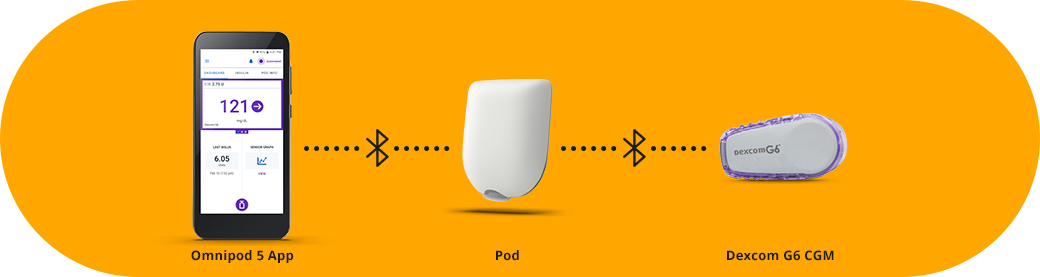
\includegraphics[scale=0.4]{diagrams/Omnipod-5_CGM_Pod_BT_1040x277.jpg}
    \caption{Diagram made by Omnipod showing the communication of the Omnipod 5.} %what can I do as another option?  I have the hardware
    \label{fig:omnipod}
\end{figure}


Another Cybernetic concept which is present in music composition of the 20th century is that of second-order cybernetics. The core differences between first and second order cybernetics is the inclusion of the observer within the cybernetic system. Rather than a completely isolated system, a person in a second-order cybernetic system is able to observe and react, altering the system and controlling the output to various degrees. In terms of musical composition, this allows for a composer to both allow for the unique characteristics of cybernetic systems, but still control the output enough to give the final result their own unique flair. One of example of this is Terry Riley's \textit{In C} or Fredrick Rzewski's \textit{Les Moutons de Panurge}. Both of these 20th century work have performers playing musical snippets, but are independent of each other. As the performers become less in-sync, they are able to make more choices that affect their performance, and how they are interacting with the group as a whole.

Cybernetic concepts such as feedback loops and automatic responses are heavily utilized in Cybernetic music. The idea of the music becoming a sort of living thing that is able to grow and change on its own, or develop a unique, self-aware character is appealing to many composers of the 20th and 21st century. Many other composers would also direct this evolving music in order to create more desirable creative results. In addition to being an augmented instrument, the Cyberinet utilizes Cybernetic principles in its design and intended uses. 



\subsection{Cybernetic Music Practices}
As previously mentioned, cybernetic principals have also been utilized in music composition. Various composers have utilized Cybernetic ideas to create music that can evolve over time. These effects can give the music a unique character and identity. Implementing cybernetic music can happen through both entirely acoustic means, as well as through computer controlled algorithms. This subsection will discuss three composers who utilized Cybernetic in various ways, as well as how those concepts were utilized within a specific composition.


\subsubsection{Herbert Brün} %% needs to be longer. Include a detailed breakdown of at least 2 seeds. Mention more about what he did in computer science. headshot.

Born in 1918, Brün was both a composer and computer scientist who focused on Cybernetic concepts in his various works. Many of these works were programmed in early coding languages such as FORTRAN which allowed Brün to incorporate both randomness and Cybernetic feedback into the music generation process. In a handful of works, such as \textit{mutatis mutandis} from 1968, would utilize random number seeds in order to create visuals which were then interpreted by musicians.

In relation to Cybernetics, Brün was influential in the development of Second-Order Cybernetics along with other scientists such as Heinz Von Forester and Margaret Mead. Second-Order Cybernetics ultimately developed into a process which is heavily utilized in Cybernetic music moving forward. In short, the main feature of Second-Order Cybernetics is the inclusion of the observer in the Cybernetic system, as opposed to them existing outside of it\cite{Scott_2nd_order_Cyber}. In relation to the creation of music, this meant that a composer utilizing this concept would be able to create a cybernetic system, and then directly influence it in order to affect the outcome.


\subsubsection{Roland Kayn} % more biography. try and find more detailed information on composition. headshot

A German born composer, born in 1933, who was heavily inspired by information sciences when creating his unique style of mainly electronic and electroacoustic music\cite{rolandKaynBio}. His earliest works to utilize the cybernetic concepts was \textit{Galaxis} (1962) for a variable acoustic instrumental ensemble and \textit{Cybernetic} (1969) for electronics. Kayn would write several more over the following years. These works incorporated cybernetic principals in what Kayn referred to as being "self-governing"\cite{rolandKaynBio} and "able to think for itself\cite{Kayn_Elektroakustische_Projekte}. In the context of Kayn's electronic music, this was present in algorithmic processes which incorporated semi-random calculations. These unpredictable results were then fed back into the system which resulted in unpredictable, autonomous results\cite{rolandKaynBio}.

\begin{figure}
    \centering % get permission for score page
    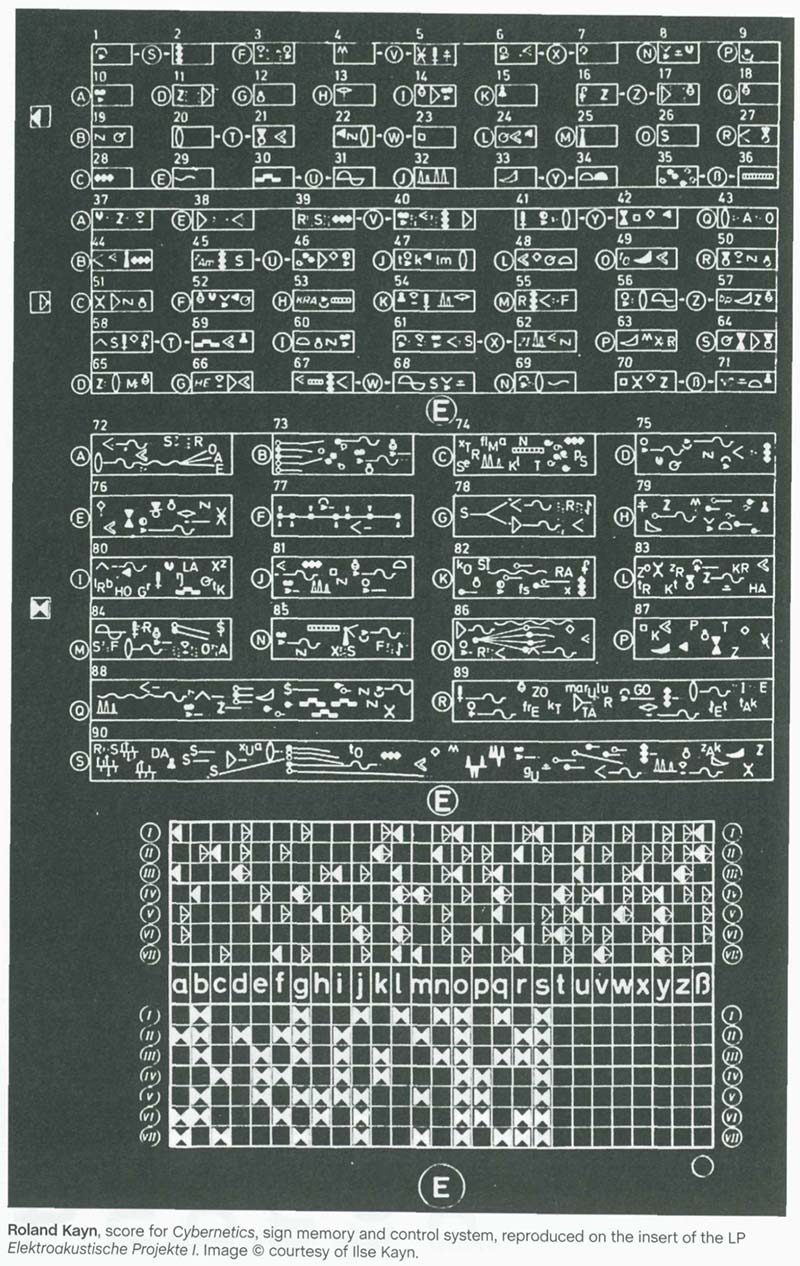
\includegraphics[scale=0.45]{diagrams/kayn_cybernetics.jpeg}
    \caption{\textit{Cybernetics I} (1969) score, Courtesy of Ilse Kayn, used by permission}
    \label{cyberneticsScore}
\end{figure}


Figure \ref{cyberneticsScore} shows one of Kayn's works, \textit{Cybernetics I} from 1969, and shows the various electronic components used to generate the sound in the top portion, and how those components interact in the bottom portion, similar to the matrices used in synthesizers of the era. Looking at the score, we can see how the output of certain processes are fed back into the system, causing the feedback loops common to Cybernetic music.


\subsubsection{Pauline Oliveros} % show page of sonic meditations
An American composer, performer, and educator, Oliveros was a founder of the San Francisco Tape Music Center and pioneer of\textit{ Deep Listening}\cite{HolmesElectronicMusic2020}. \textit{Deep Listening} is a school of thought at method of listening described by Oliveros as:

\begin{quote}
    ... For me [Oliveros], Deep Listening is a lifelong practice. The more I listen the more I learn to listen. Deep Listening involves going below the surface of what is heard, expanding the whole field of sound while finding focus. This is the way to Connect with the acoustic environment, all that inhabits it , and all there it.

    For others, Deep Listening is a practice consisting of listening and sounding exercises and pieces I and others have composed since 1970. The results are proceeded by a group of discussions in workshops and retreats. 

    Deep Listening is for musicians as well as participants from other disciplines and interests. Previous musical training is not required\cite{cultureandHumanity2002}.
\end{quote}

At its core, the idea of \textit{Deep Listening} itself is a cybernetic practice\cite{gordosOliverosCybernetics}. This is because of \textit{Deep Listening}'s core principle of listening to how you listen. The act of a system responding to itself in a feedback loop is a core concept in cybernetics. In relation to Olivero's music, the concepts of deep listening and cybernetics can be clearly seen in her tape improvisations of the 1950's and 60's. In these works Oliveros along with a variety of collaborators would record themselves improvising, then listen to the recording and discuss what they heard. Following this the group would repeat the process until they were pleased with the results\cite{gordosOliverosCybernetics}. 

\begin{figure}
    \centering % get permission: Pauline Oliveros. Credits: Bert Johnson. But who do I email? there are many Bert JOhnsons https://eastbayexpress.com/avant-garde-luminary-pauline-oliveros-listens-deeply-to-the-berkeley-art-museum-1/
    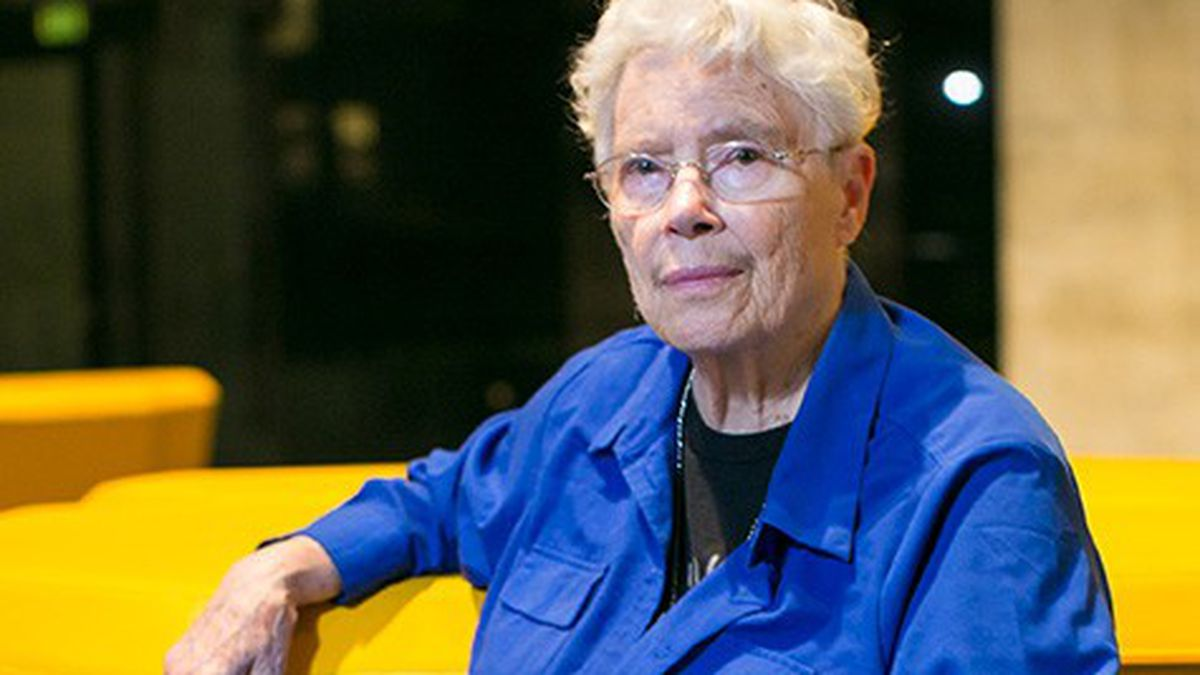
\includegraphics[scale=0.25]{diagrams/oliveros.jpg}
    \caption{Pauline Oliveros}
    \label{fig:oliverosHS}
\end{figure}

Another series of works with cybernetic principles is Olivero's \textit{Sonic Meditations} (1974). \textit{Sonic Meditations} is a collection of 25 different actions intended to cause the performer to intensely focus on their action, the sounds around them, and the sounds of their actions\cite{OliverosMeditations}. The instructions are all given as text have been performed in a traditional setting or individually, but in the score Oliveros intends to remove nay connotation of traditional performance and focus on the sound through \textit{Deep Listening.} 

These prompts range in complexity and specificity ranging from talking a walk with as quiet of steps as possible to singing pitches in groups until a single pitch is established. There are also more complex activities focused on breathing and the acts of making, listening to, imagining, and remembering sounds\cite{OliverosMeditations}. By actively guiding the performer through the \textit{Deep Listening} activities, all of the cybernetic principles of \textit{Deep Listening} become present in the music performance as well. All 25 pieces have in some way the performer listening to a sound occurrence and responding by altering their actions to change the sound environment.

\subsubsection{Onyx Ashanti} 
Onyx Ashanti is a modern composer, performer, and inventor largely known for developing "beatjazz", an electronic gesture controller used to utilize a mixture of improvisation, looping, and gestural control. These gestures are incorporated through his instruments, which directly attach to the human body. A few sensors are even located within the performer's mouth. These particular arrangements of data work to remove some of the traditional aspects of music creation and performance and allow for the creation and control of audio to happen solely through the direct measurement of the performer.

The Beatjazz controllers are held in the performer's hands and utilize accelerometers in order to track the positional data of each hand, FSRs to monitor finger pressure both as buttons and continually, and a wind sensor placed in the performer's mouth\footnote{Stock non-withstanding, all of the parts for the original Beatjazz controller can be ordered as a set directly from.}. The system is controlled through a computer running the various software patches for each performance. In terms of feedback, Beatjazz utilized a paired smartphone in order to act as a GUI for the performerer. LED's on each sensor allow for the user to easily see which parameter they are controlling using the following setup:

\begin{table}[]
    \centering
    \begin{tabular}{|c||c|}
    \hline
      red   & drums \\
      \hline
      blue   &  bass\\
      \hline
      green & chords \\
      \hline
      orange & leads\\
      \hline
      purple & pads\\
      \hline
    \end{tabular}
    \caption{LED color feedback in BeatJazz}
    \label{tab:bjLEDs}
\end{table}


The most interesting aspect of Beatjazz is that it removes the need for a traditional instrument or control interface in order to create music in real time. By ergonomically fitting onto the performer, their physical actions are directly used in order to alter the musical environment. By altering how they are moving, the performer can directly change what samples are being used and how they are being digitally processed. This allows for Beatjazz to function cybernetically both in the popular culture and scientific uses of the word. However, because of how it is utilized on the body, it is less of an augmented instrument than something completely new, which has many common similarities with digital augmented instruments.

\section{The Cyberinet}
Taking everything up to this point into consideration, and the main definitions and goals of the Cyberinet can be clearly broken down. When comparing it to the digitally augmented instruments, there are several features that the Cyberinet iterates on, and several that it intentionally does not embody.

In relation to MIGSI, the Cyberinet is also designed to be minimally invasive. While a performer can interact with the instruments in novel ways to create interesting effects through the various sensor data, utilizing MIGSI and the Cyberinet by itself does not impede the traditional performance practice of the performer. Other than instrument compatibility, the main way that the Cyberinet differs from MIGSI is that the Cyberinet is designed to be easily installed and removed, allowing the performer to choose whether their instrument is completely acoustic or augmented. While a performer can choose not to connect MIGSI to the computer, making it acoustic, the MIGSI sensors are not easily removable. Looking at figure \ref{fig:MIGSI}, the sensors are bolted or otherwise securely attached to the base trumpet. When defining the Cyberinet, it was a goal to create a device that would not require a permanent alteration to the instrument, and was in fact able to be quickly implemented in a performance setting like a brass mute. Permanent alterations could be potentially off-putting to musicians. who may be unable to afford a second instrument to augment, or are otherwise unwilling to permanently alter their horn.

The Hyper-Flute is able to interact with a variety of devices or the computer through its Metalab interface and a MIDI port\footnote{This is my favorite feature of the Hyper-Flute, even if the interface results in an additional hardware purchase needed in order to perform with the instrument on top of already having to permanently add the sensors to your flute or buying a separate one to augment.}. While not identical, the Cyberinet software is intended to be able to interact with a variety of hardware and software using Max as the main platform. However, the large number of wires hanging from the Hyper-Flute are both distracting in a performance setting, and can potentially obstruct the performer's movement\footnote{A portion of this drawback is due to the development of more powerful and smaller digital sensors in the 20 years between the development of the Hyper-Flute and the Cyberinet}. The Cyberinet wirelessly communicates with the computer with only external wires needed to connect to optional expansion sensors or to charge the Cyberinet.


Of the discussed instruments, the SABRe is the device most closely related to the Cyberinet. This is in no small part due to the fact that they are designed to augment the same instrument. This also lead to common types of sensors between the two as the sensors are monitoring the same actions. These similarities require a more in-depth breakdown in order to properly differentiate the two devices. Despite being designed for the same instrument, each device has its own unique positive and negative aspects.


\begin{table}[]
    \centering
    \begin{tabular}{|c||c|}
    \hline
     SABRe & \textbf{Pros}: small, completely wireless, easily removable. \\
         & \textbf{Cons}: no modularity, cost, \\
         & buttons difficult to use without the thumb expansion.\\
         \hline
    Cyberinet & \textbf{Pros}: integrated within the instrument,\\
    & expandable with add-ons,\\ 
    & relatively inexpensive to produce, open source-components.\\
    & \textbf{Cons}: less easily removable, \\
    & some wires involved, annoyingly complex to install.\\
    \hline
    \end{tabular}
    \caption{Pros and Cons of the SABRe and Cyberinet}
    \label{tab:sabreCyberinetProCons}
\end{table}



in regards to the SABRe, while extremely simple to set up and utilize, the lack of additional sensors could hamper potential uses. The chosen sensors are all useful in collecting clarinet performance data, but it cannot be customized outside of adding two buttons to the version one system. To help avoid this potential limitation in the Cyberinet, the Cyberinet is designed to be able to attach an expansion unit with an additional sensor\footnote{This was also done in order to help differentiate the Cyberinet from the SABRe in terms of design and functionality.}. These sensors are all compatible with OEM components and utilize the same voltage ranges. This allows them to be easily swappable in a performance setting.

The final aspect of the SABRe that the Cyberinet intentionally differs from, other than physical design, is the cost. The initial version of the Cyberinet is designed to be completely open-source, utilizing OEM components. While this does increase the overall size of the Cyberinet, it results in a final unit that is significantly cheaper to manufacture than the SABRe. The initial version of the SABRe retailed for approximately €500. All of the components for the Cyberinet: sensors, PCBs, connectors, and 3D printer filament cost approximately \$120. A retail price would be higher, but still significantly lower than that of the SABRe. Even with a 100\% markup, the final cost of the Cyberinet, is less than half that of the SABRe. By having a cheaper development cost, the Cyberinet has a lower cost-of-entry wall, making the unit significantly more accessible than the SABRe. In fact, is a person already has a 3D printer, then they can completely create and program a Cyberinet from scratch for only the cost of the materials.

%%%%%%%%%%%%%%%%%%% define the categorizations?
In the article \textit{Mapping, in digital instruments}\cite{vanNortMapping2007}, Van Nort describes Digital Musical Instruments as being either implicit or explicit in regards to their use of the control data. Where explicit designs are analytically described and implicit interactions are applied through some sort of training\cite{vanNortMapping2007}. In his paper, Van Nort goes on to describe a handful of other interactions between the data being collected and the sound being produced. Using the terms defined there, the Cyberinet can be described as using an implicit, dynamic, and continuous use of the performance gestures for its computer augmentation. Controls are based on clarinet performance practice and not a new set of skills, the sensor types can change through its designed modularity, and the sensor data is continuously being collected while in use. There is also a multiple layers of mapping between the raw data and what is utilized to produce sound. This is to help further draw correlations for gesture recognition as well as ease of use when programming.

Looking back at the instruments discussed previously in this chapter, we can see many of the instruments share similarities with the Cyberinet in this design choice. While none of the aforementioned instruments would be considered dynamic for exactly the same reason as the Cyberinet, they all collect continuous data using implicit means. The Hyper-Flute specifically has the ability to the data to MIDI for use in other devices,but all four instruments can have the data further mapped within the Max software. Due to the ability for the mapping to change within the software environment for all four of these instruments, each one is capable of adapting and changing the mappings in real time, an act which Van Nort describes as the mapping becoming playable itself\cite{vanNortMapping2007} in a fashion similar to the idea of Second-Order cybernetics.

As stated, the Cyberinet can be defined as a new augmented instrument which can be implemented with a standard B-flat clarinet. This augmented instrument collects data from various embedded sensors and transmits the data to a nearby computer while the performer plays the instrument traditionally\footnote{Or not. The gestures being captured can be experimented with in order to develop unique sound possibilities.}. The sensors can be adjusted in a semi-modular fashion; by adding or removing expansions to the two main ports on the main unit. The Cyberinet is intended to be affordable to produce, using OEM components with open-source resources. This is to allow for more accessibility to a wider range of performers and composers wishing to work in electroacoustic music. Lastly, because of the Cyberinet being able to control audio processing through the act of performing on the clarinet, it brings a level of Cybernetic awareness to the performer as well. A performer will be able to play and hear how their actions are influencing the music and either positively or negatively reinforce that control by adjusting their playing in real time. 

But how exactly will the performer be able to influence their playing? A performer composer or performer could create specific movements at specific times to trigger an effect, this could be pre-planned or improvised. A student could monitor the data while learning the instrument to check their positions and breath control. The potential for sound and control options are astronomically high, but there are a handful of useful methods and interactions envisioned by the author, which can help guide newcomers to the Cyberinet. Before we dive into exactly how it is used, Let us first discuss how the Cyberinet was designed, assembled, and programmed.


\chapter{Building the Cyberinet}
When developing the functionality of the Cyberinet, the steps defined by Miranda and Wanderley in their book\cite{miranda_Wanderley_instrumentControl_2006} helped to organize and streamline to process. Paraphrased, that process is shown in table \ref{fig:DMIProcess}. This chapter will utilize the process given here by Miranda and Wanderley as a road map to breakdown exactly how the Cyberinet was designed and created.

\begin{table}[]
    \centering
    \begin{tabular}{|c||c|}
    \hline
     Step 1    & Determine gestures that will control the instrument. \\
     \hline
     Step 2    & Determine how to capture the gestures for use within the system. \\
     \hline
     Step 3    & Define the specific sound creation processes that will be controlled by the sensors. \\\hline
     Step 4    &  Map the gesture control data to the desired sound-creation parameters.  \\
     \hline
     Step 5    &  Decide on the feedback mechanisms for the performer to be able to respond to.\\
     \hline
    \end{tabular}
    \caption{Digital Instrument Design steps as defined by Miranda \& Wanderley\cite{miranda_Wanderley_instrumentControl_2006}.}
    \label{fig:DMIProcess}
\end{table}


\section{Control Gestures \& Gesture Sensing}
The main control parameters for the Cyberinet are those present traditional clarinet performance. While conceptualized as something new, the Cyberinet, as an augmented instrument must still retain its identity as the original instrument\cite{miranda_Wanderley_instrumentControl_2006}. Towards this goal, a breakdown of a clarinet performance is needed in order to see which gestures are naturally occurring. These are not the only gestures possible when utilizing the Cyberinet, but serve as a starting point for developing intentional gestures that can be utilized when composing new works.

In a clarinet performance, there are a handful of easily measurable actions that occur. The main ones chosen for the Cyberinet are performer movement, which can often be tied to expressiveness\cite{wanderleyClarinetGesture2005}, and performer volume, which can be tied to the volume of air flowing through the instrument. Other parameters exist as well such as determining which keys are being pressed, how hard the keys are being pressed, and which pitch is being produced by the clarinet. While potentially interesting, measuring these data points in real time becomes more problematic due to the necessary placement of sensors and microphones which would potentially impede the performance or alter the instrument into something similar, but distinct from the original clarinet. Because of these reasons, the movement gestures are the primary focus of the Cyberinet's main unit, followed closely by measuring the air flowing through the horn.

When performing on the Clarinet, the performer generally will pivot or sway horizontally (left-to-right) as they are performing. These motions are the primary focus of the gyroscopic and position sensors as they are both common to see, and province the largest range of data of the sensors discussed here. Performers can also lean forward or back while performing, necessitating a need for a second degree of motion in the sensor. It is relatively unlikely that a performer will have significant alterations to the vertical height of the instrument while performing, conceptualizing the Cyberinet as a unique instrument opens up the possibility of performance control to traditionally unused actions. Because of this, the Z-axis is also monitored by the gyroscope and accelerometer. 



The second sensor embedded within the Cyberinet's main unit is a differential airflow pressure sensor. This sensor was chosen as a way to measure the airflow within the instrument. As a performer creates notes at different dynamics, the volume of air flowing through the instrument will change. By comparing the pressure within the horn with the air pressure outside of the instrument, these values can be easily calculated as a number to utilize in the code.

With the general gestures and sensors determined, the next step is to work out a more specific list of gestures. In 2005 Wanderley et. al conducted a study in order to determine both what expressive gestures were present in Clarinet performance, as well as how these gestures can affect music performance and perception\cite{wanderleyClarinetGesture2005}. The gestures identified in this study serve as a wonderful baseline for identifying specific movement possibilities. Summarized, these natural expressive performance are listed in table \ref{tab:generalGestures}.

\begin{table}[]
    \centering
    \begin{tabular}{|c||c|}
    \hline
       Instrument Movements  & Bell, vertical and circular \\
       \hline
        Upper Body Movements & Head, vertical \\
        & Shoulders, vertical \\
        & Back, curl inwards \\
        & Arms, raising elbows \\
        \hline
        Lower Body Movements & Waist, bending \\
        & Knees, bending \\
        & Feet, walking \\
        & Weight shifting, left and right\\
        \hline
    \end{tabular}
    \caption{Identified Gestures by Wanderley et. al\cite{wanderleyClarinetGesture2005}, divided by body area.}
    \label{tab:generalGestures}
\end{table}

These natural gestures are all able to be measured with the Cyberinet. Rotations are easily picked up by the gyroscope, movements by the accelerometer, and breath by the airflow sensor. While Wanderley et. al did not measure the airflow in their study, it is still an important sound-producing gesture\cite{miranda_Wanderley_instrumentControl_2006}. Each of the gestures listed above as well as a handful of airflow gestures were tested with the Cyberinet in order to calculate the various sensor responses to various scenarios. This data was then used to create Max objects that can utilize both slower, gradual movements, as well as faster ones that can be be interpreted as a single action.

%should I move the breakdown of geasutes adn thier data visualizations to here?

\subsection{Gesture Mapping}

Because of the modularity of the programming environment, a single gesture sensed by the Cyberinet can be mapped to anything within Max. This leads to a few unique concerns; mainly the idea of determining the most effective parameters to map to an effect. This design feature is to create a wide variety in potential outcomes without the need for the performer to learn an equally large number of control actions. This potentially overwhelming amount of options is made more manageable with the use of a normalized value range for the sensors and a collection of Max objects that either process sound or help prepare the use of the data for use in other ways. 

When deciding which gesture is effective for an effect depends on a few parameters. The first one is purely mathematical; if a parameter utilized exponential changes in values, then a similar data profile will prove more effective than others; the same is true for linear data mapping. A quick gesture will prove best for a quick change or process within Max, whereas slower changes in data values are better applied to continuous audio processed\footnote{Such as activating a gate with a short gesture versus controlling the pitch of a synthesizer with a longer movement gesture.}. 

The second parameter depends on the performer. People will naturally perform differing natural movement when performing\cite{wanderleyClarinetGesture2005}, which could result in varying sensor responses between users. Because of this an object was created in order to adjust the scaling of values as needed for each performer. This way, with minimal setup, the sensitivity of each continuous sensor in the Cyberinet can be scaled to match the movements of varying performers in order to achieve a consistent performance effect.

\subsubsection{Mapping Gestures to Max} %was previously 3.3 before I moved it.

The idea of mapping physical gestures to the sound production/processing created by an augmented has already come up a few times. While indeed this can be done haphazardly or randomly, in order to properly utilize the cybernetic capabilities of the Cyberinet (or any other digital musical instrument), the performer must be able to respond to the current state they are in and create either a positive or negative feedback loop to maintain, grow, or diminish the current state. In order to do this, it is important to identify gestures being used and how they are mapped. Generally speaking a gesture can be traditional or experimental in nature. Table \ref{tab:generalGestures2} is a reproduction of table \ref{tab:generalGestures}. Each of the gestures listed here have been analyzed and visualized for easier application to sensors.


\begin{table}[]
    \centering
    \begin{tabular}{|c||c|}
    \hline
       \textbf{Instrument Movements:}  & Bell, vertical and circular \\
       \hline
        \textbf{Upper Body Movements:} & Head, vertical \\
        & Shoulders, vertical \\
        & Back, curl inwards \\
        & Arms, raising elbows \\
        \hline
       \textbf{ Lower Body Movements:} & Waist, bending \\
        & Knees, bending \\
        & Feet, walking \\
        & Weight shifting, left and right\\
        \hline
    \end{tabular}
    \caption{Identified Gestures by Wanderley et. al\cite{wanderleyClarinetGesture2005}, divided by body area.}
    \label{tab:generalGestures2}
\end{table}

To create this data, the CNET.gestureVisualizer object was used to record the sensors values while the movements were performed three times each. The data was then averaged and graphically represented with the multislider object in Max. The categorization of the gestures was based on this visual representation. When looking at all of the data points, the oldest points are presented on the right of each graph, and the newest points are on the left. Because of the manual trigger to start and stop recording, extra noise is present on the right-most side of each graph. 

Throughout all of the data graphs, the Gyroscopic Z-axis values appear more sensitive than the majority of the others. This is due to the positioning of the sensor on the instrument. Longitudinally, all of the motion sensors of the Cyberinet are close to the center of motion in the Cyberinet. However, transversely the sensor is located approximately 9 inches away from the center of motion\footnote{The center of motion is considered to be the thumb-rest/neck-strap attachment point in the center of the instrument.}. Because of this larger distance, the sensors which respond to that axis will register a larger range of motion. This can be adjusted slightly by rotating the Cyberinet main unit on the horn, but utilizing CNET.rangeSet will better scale the values as desired. All of the graphs shown are utilizing unaltered data from CNET.receive.

\begin{figure}
    \centering
    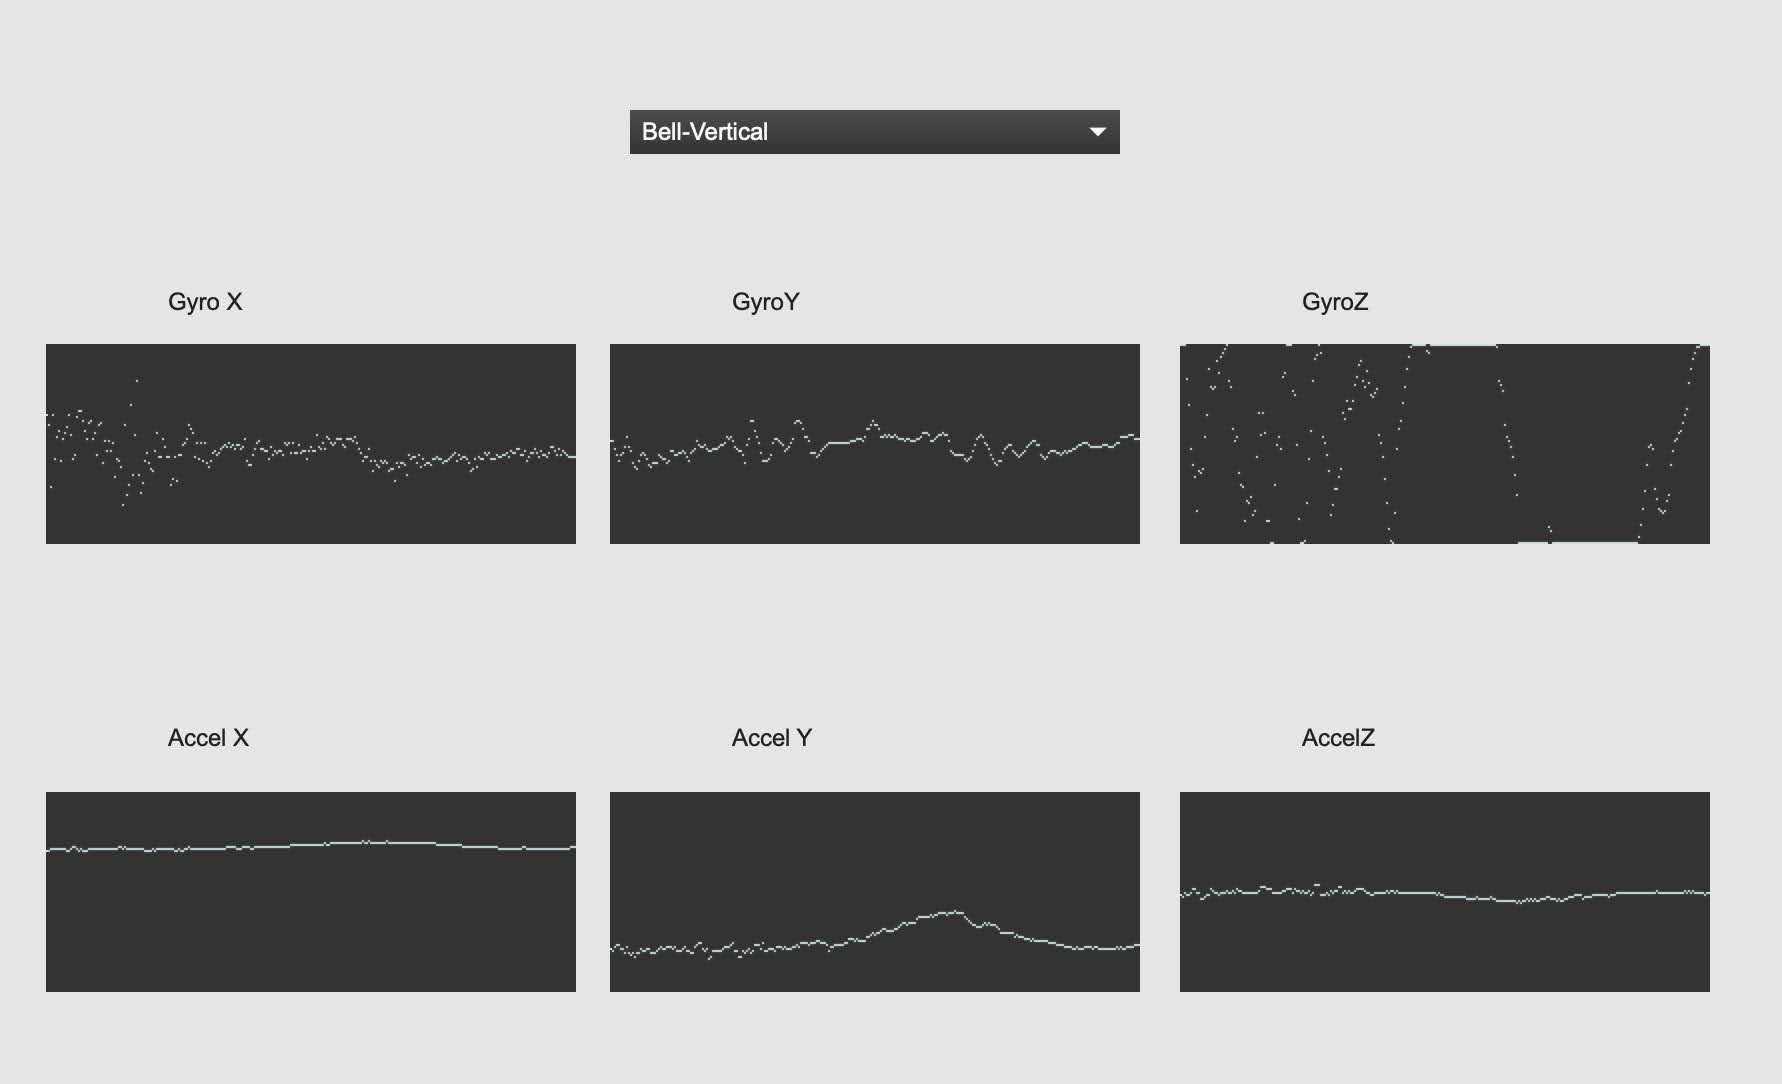
\includegraphics[scale=0.25]{diagrams/gestureData/bellVert.png}
    \caption{Raising the bell expressively.}
    \label{fig:bellRaiseData}
\end{figure}

When raising the bell, a gentle slope can clearly be seen in the accelerometer's Y axis as one would expect. 

\begin{figure}
    \centering
    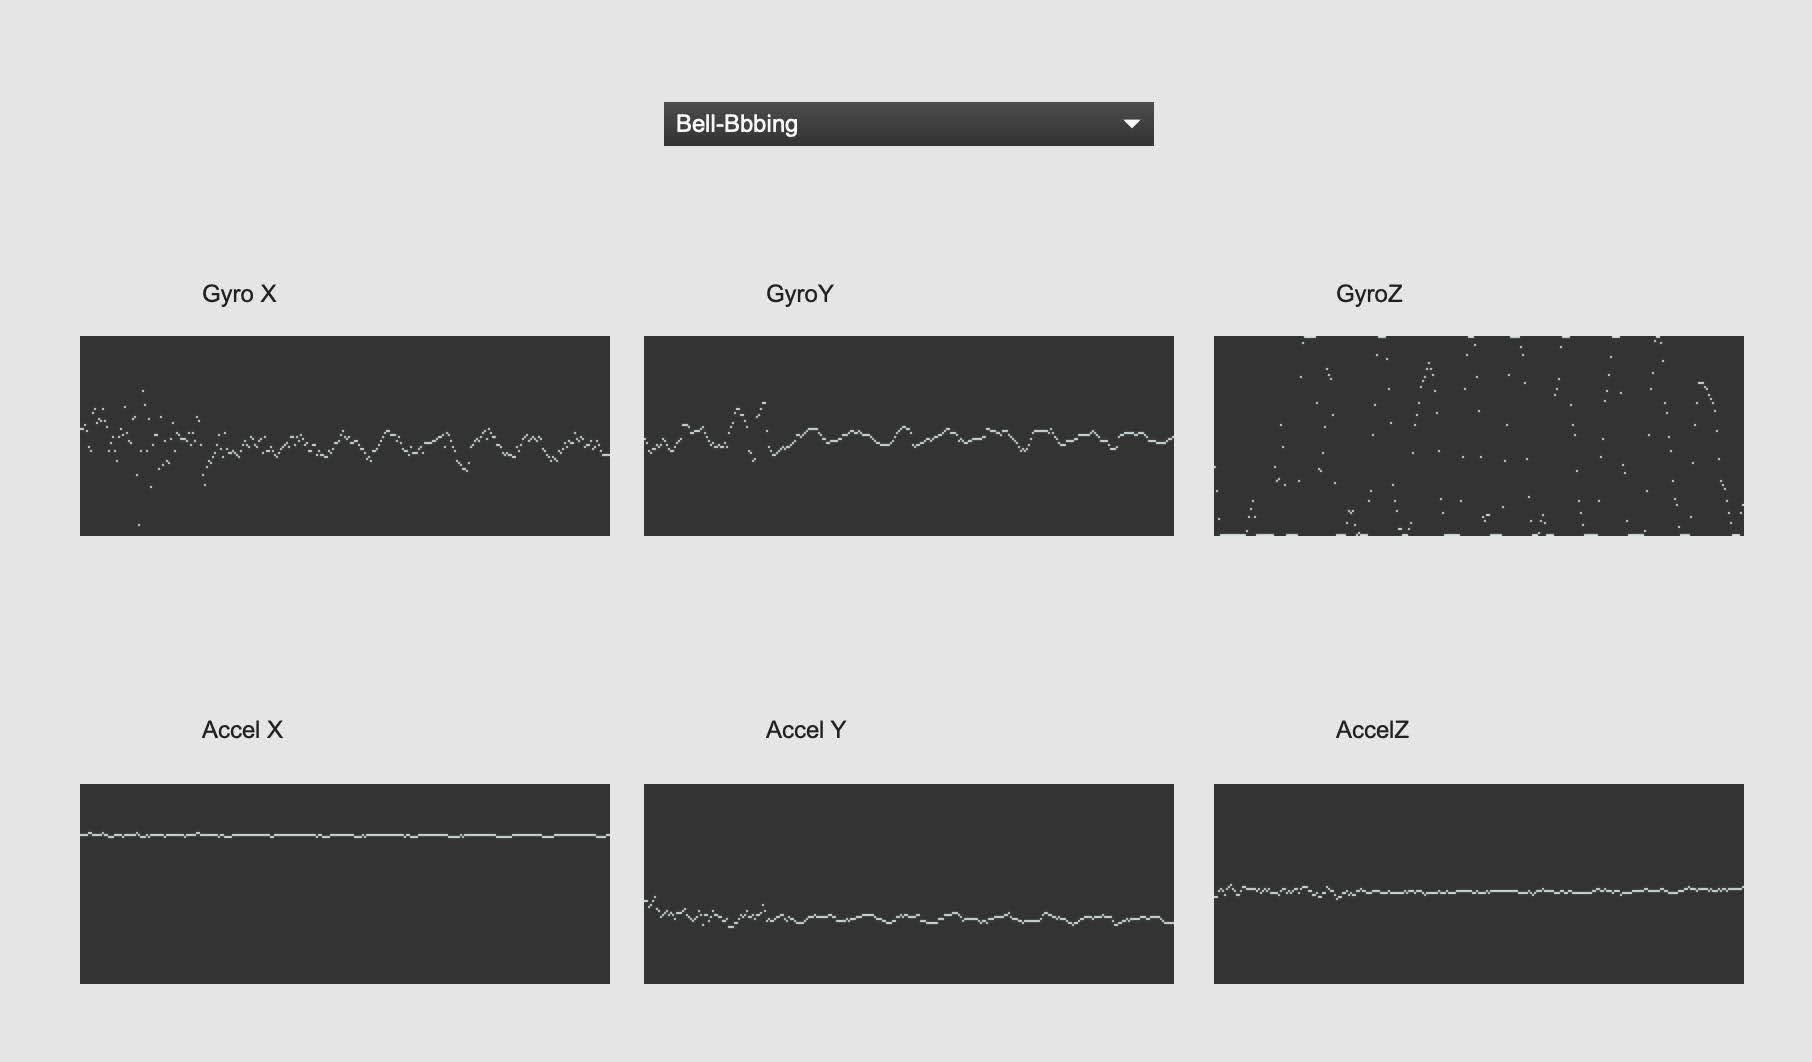
\includegraphics[scale=0.25]{diagrams/gestureData/bellBob.png}
    \caption{Small bobbing of the Cyberinet bell.}
    \label{fig:bellBobData}
\end{figure}

When bobbing the instrument bell, a clear bump appears in every sensor, similar to the single expressive raising of the horn. By focusing more on horizontal or vertical movements, different sensors will have larger slopes in their data. When testing, the bell movement was approximately four-six inches. Larger bobs will result in larger data spikes.

Mathematically speaking, this relationship between movement size and speed can be easily calculated by working with the slope of the graphs. Taking into account any offset from the sensor's 0-point, moving a large distance or moving quickly will result in a grater change of data values.

\begin{figure}
    \centering
    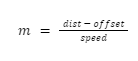
\includegraphics{slopeEqu.png}
    \caption{Equation for calculating slope of gesture graphs}
    \label{fig:mequSlope}
\end{figure}

In practice, when repeating the same movement but highly exaggerated past a natural expressive limit, changes in data become more clear and useful when utilizing the data within Max. 

\begin{figure}
    \centering
    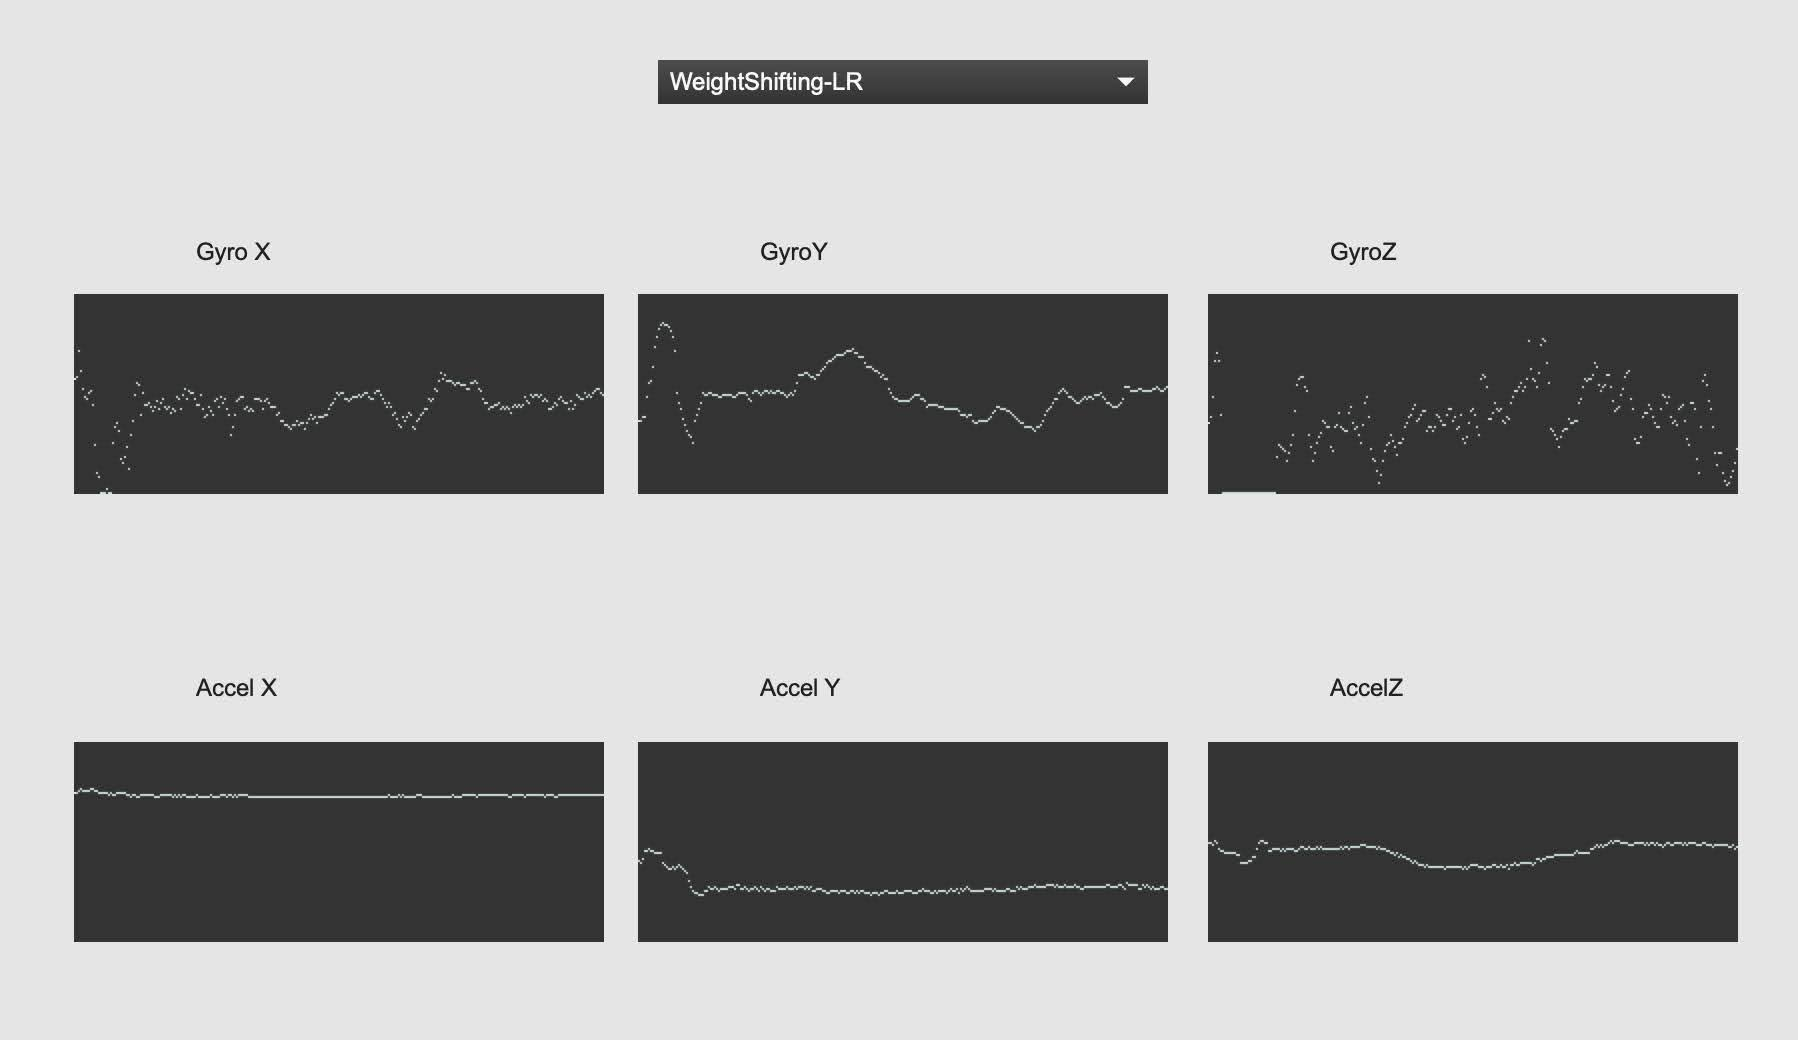
\includegraphics[scale=0.2]{diagrams/gestureData/weightshifting.png}
    \caption{Horizontal Movements in two directions.}
    \label{fig:exHor}
\end{figure}

\begin{figure}
    \centering
    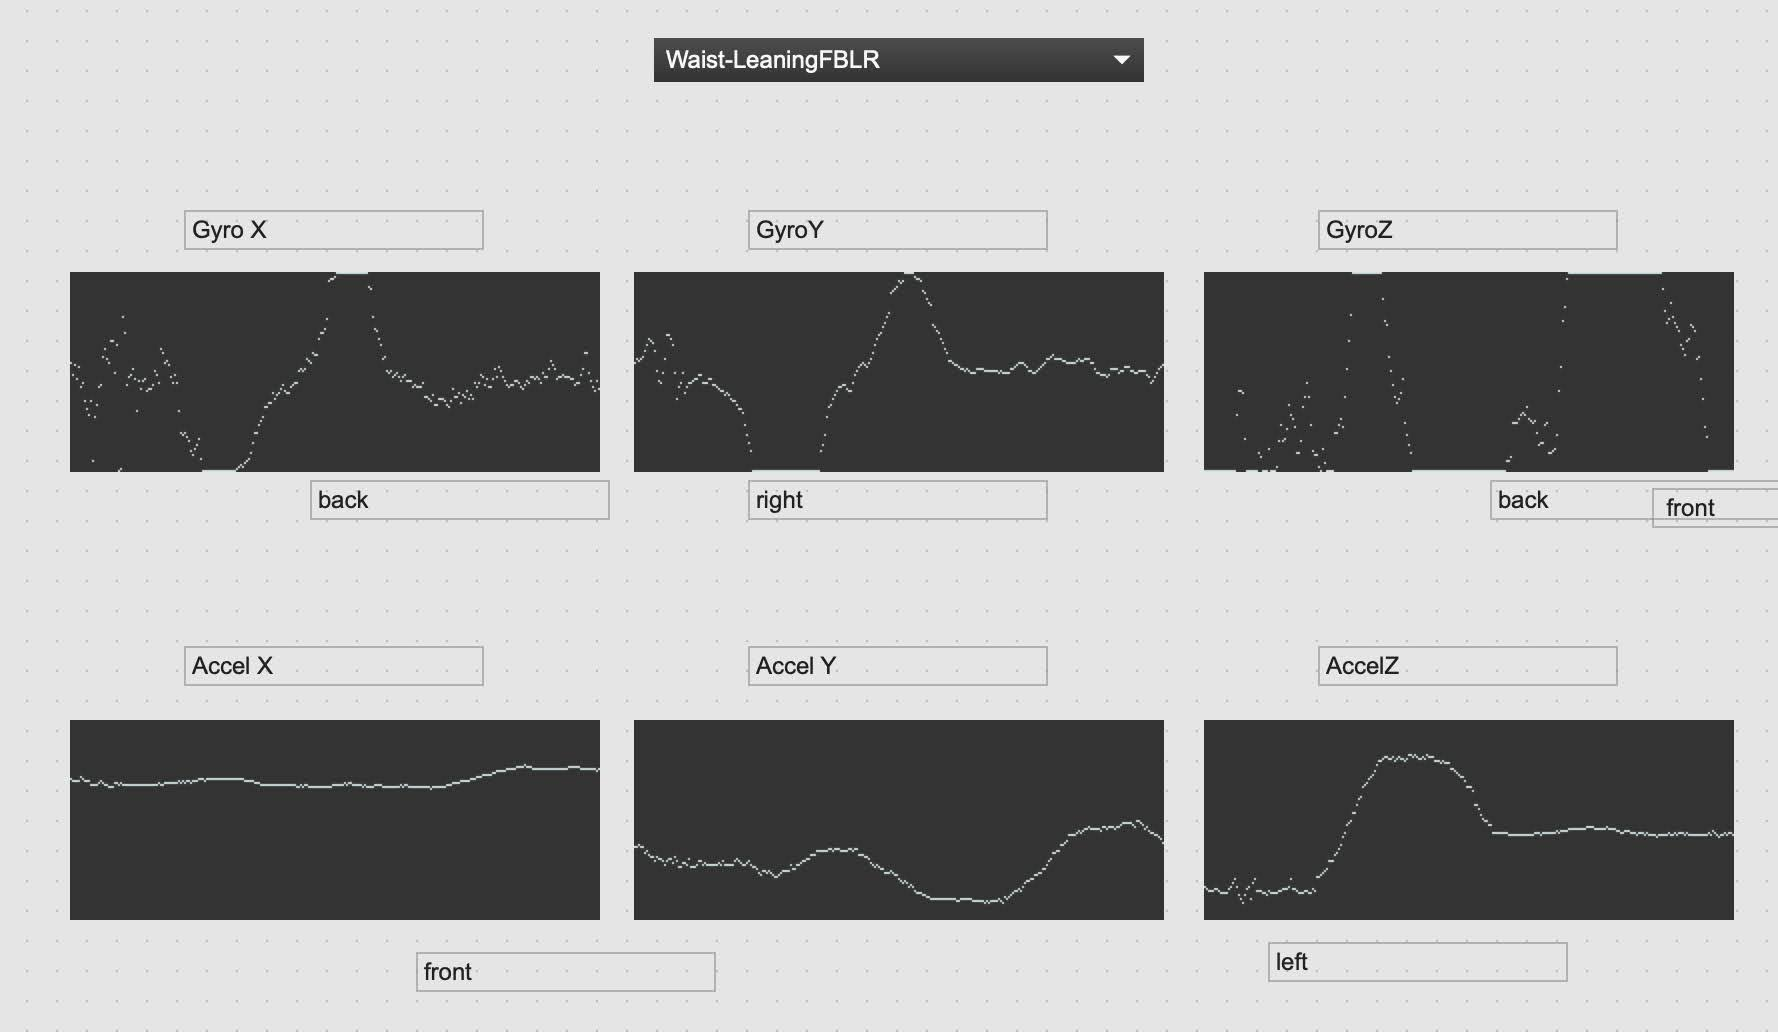
\includegraphics[scale=0.2]{diagrams/gestureData/waistLeaning.png}
    \caption{Exaggerated movements in four directions.}
    \label{fig:exHor}
\end{figure}

Air flow gestures have not been recorded in the same way was the movement gestures have. This is because breath control is intrinsically linked to the traditional clarinet performance. As dynamics increase, the values also increase as more air is flowing through the instrument, but a performer can easily control how quickly or slowly the air changes which inherently allows for more intimate control of the sensor. While performing, this range would be tightly attached to the dynamics of the performance, making it impossible to significantly alter the airflow without also altering the dynamics.

% data numbers and pictures here


 When looking at traditional gestures that occur naturally\cite{wanderleyClarinetGesture2005}, data changes are observed, but many of them are relatively static. This is to be expected as traditional clarinet performance encourages minimal movements and no rotations of the horn, so when attempting to adhere to traditional practice, the sensor data may prove relatively static. When intentionally utilizing either exaggerated gestures as measured by Wanderley et. al or more experimental movements can take more advantage of the Cyberinet's sensors.

\begin{figure}
    \centering
    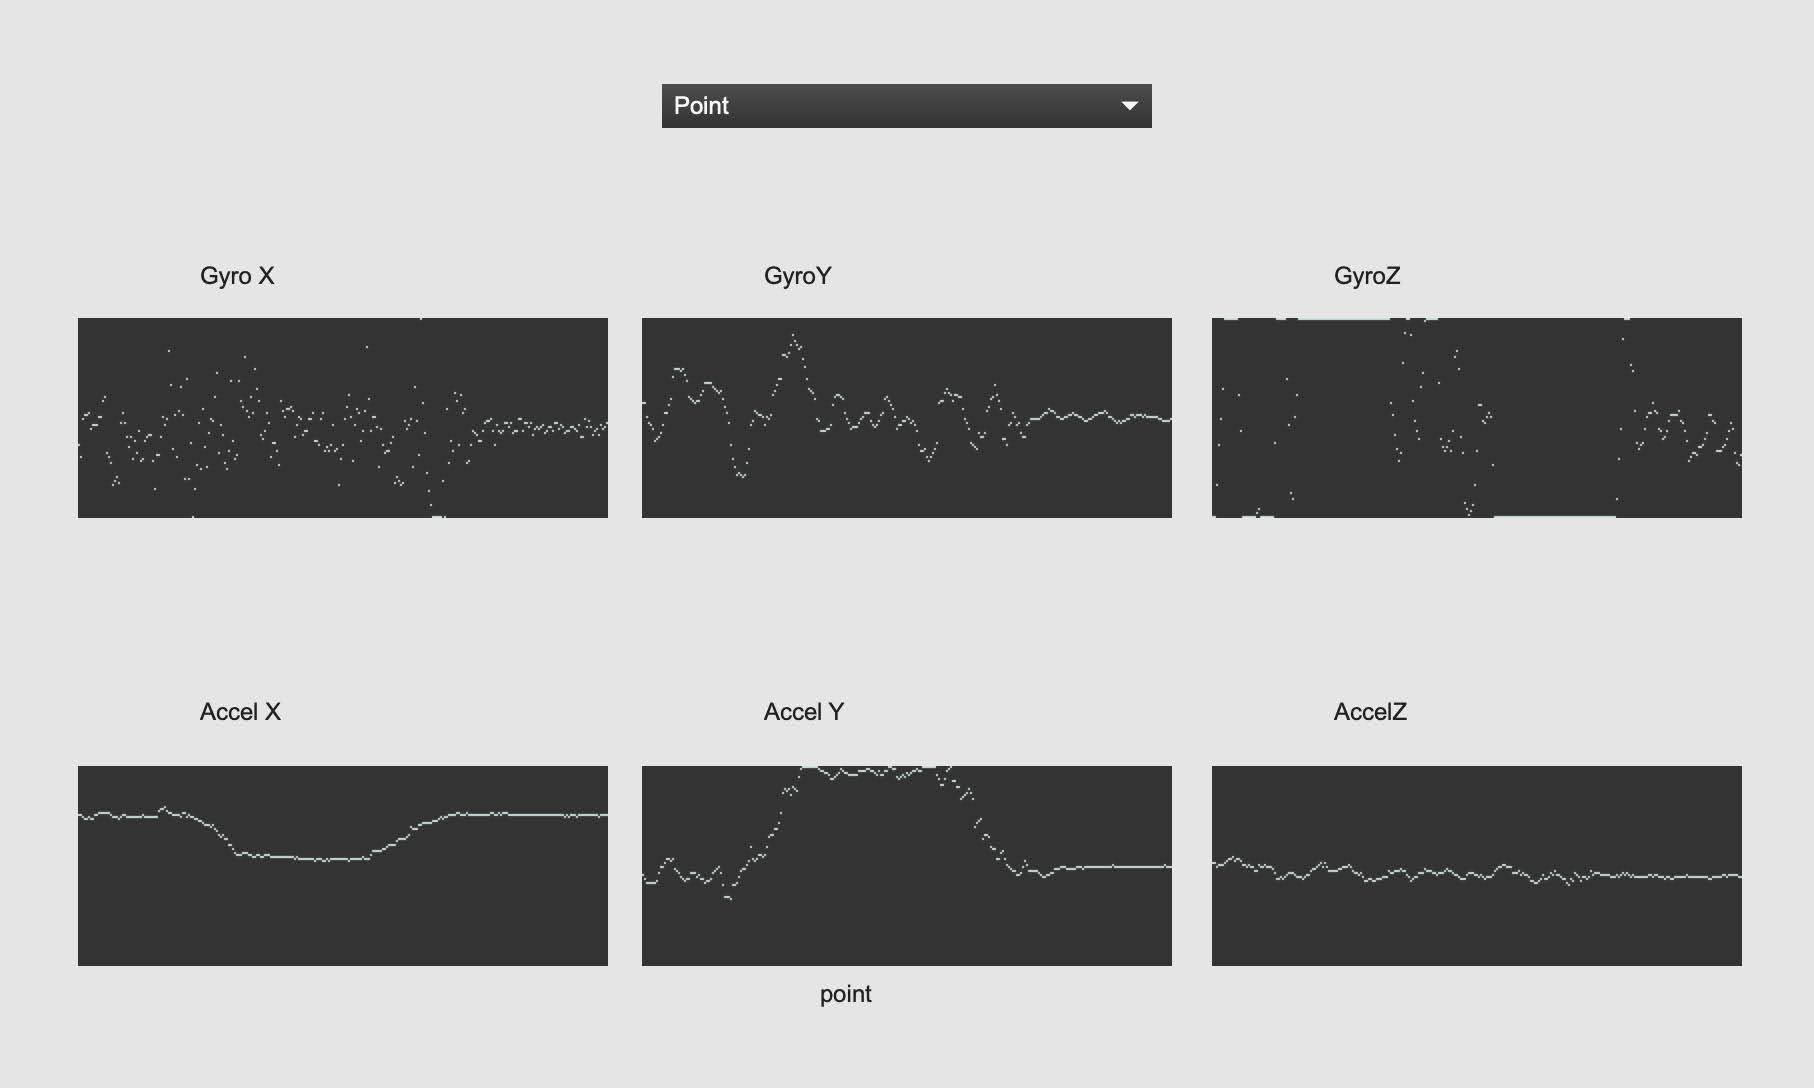
\includegraphics[scale=0.2]{diagrams/gestureData/pointing.png}
    \caption{Pointing the mouthpiece towards the audience.}
    \label{fig:pointData}
\end{figure}

For the gesture shown in figure \ref{fig:pointData}, the mouthpiece was removed from the mouth and pointed forward towards the audience, then returned to playing position. The most clear showing of this has been highlighted, and shows a clear beginning and end to the gesture. Figure \ref{fig:clotRotate} shows data from holding th instrument at arm's length and rotating it 360 degrees in a circle. The high values in the gyroscopic Y-axis show the direction, while all of the accelerometer data moves down and back as the horn passed 180 degrees and began to return to the initial positioning.

\begin{figure}
    \centering
    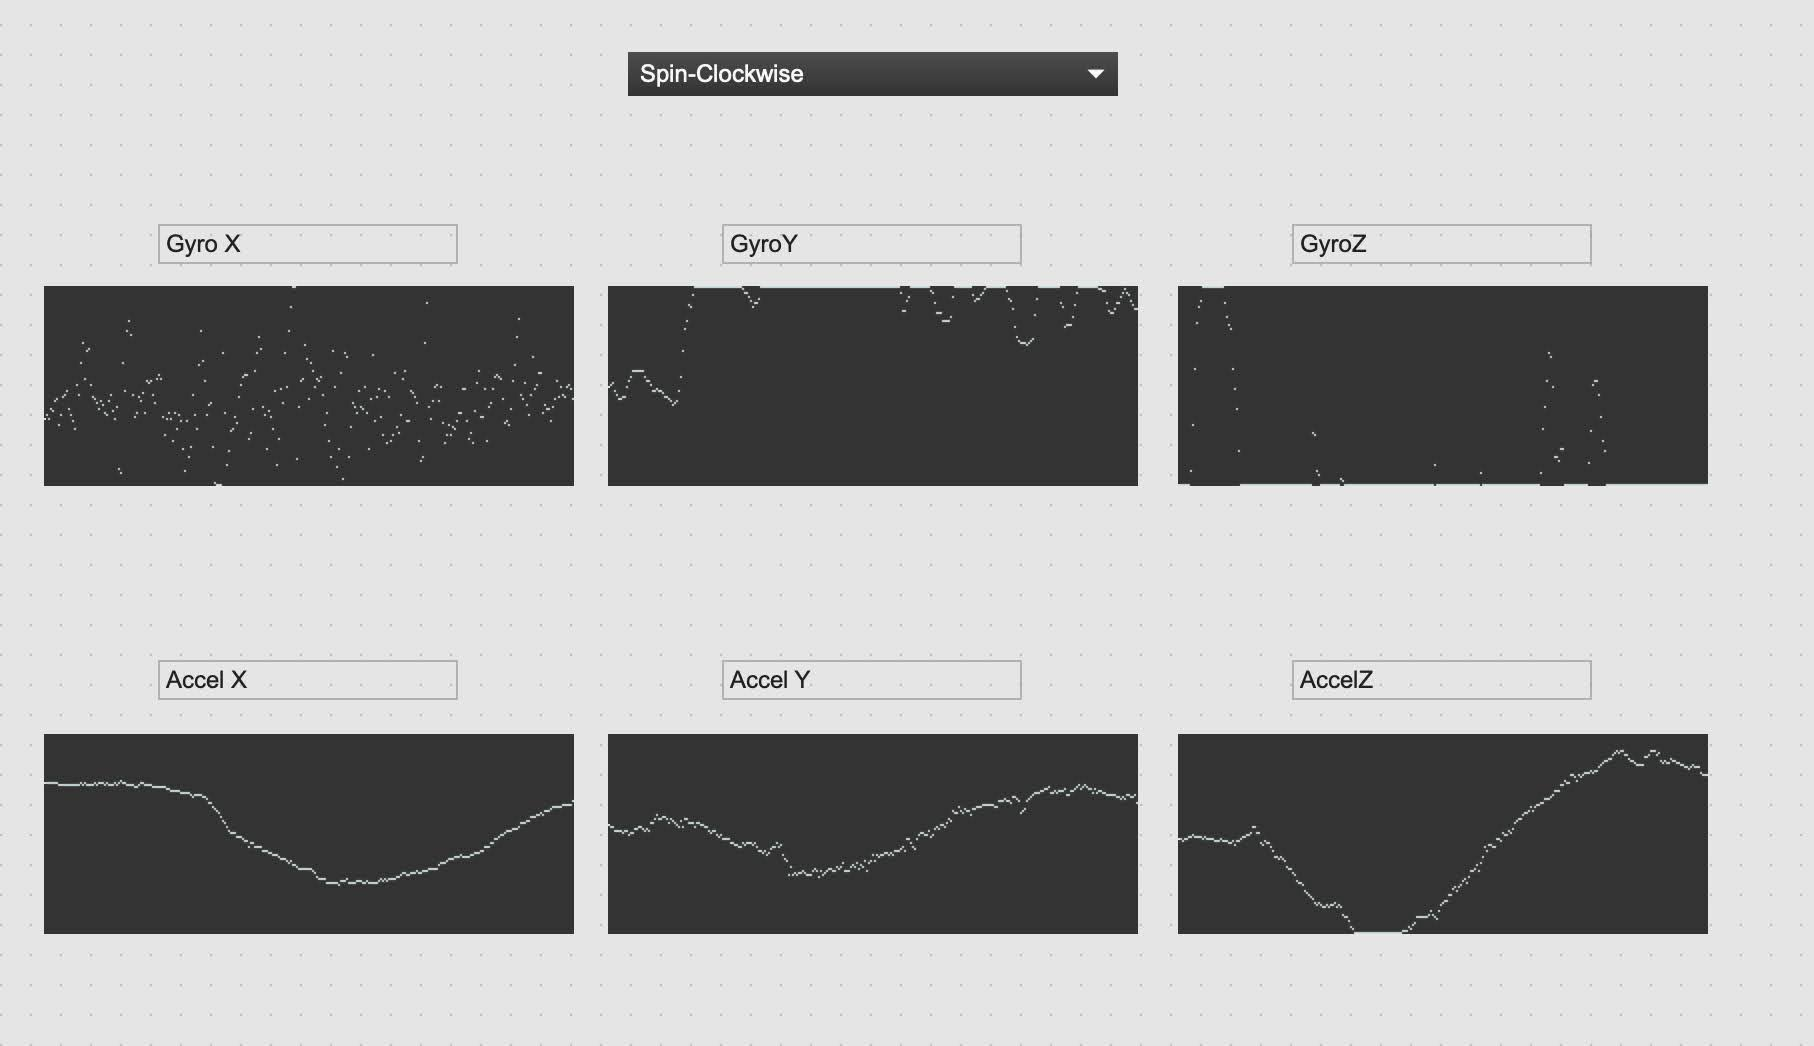
\includegraphics[scale=0.2]{diagrams/gestureData/spin Clockwise.png}
    \caption{Clockwise Rotation of the Cyberinet.}
    \label{fig:clotRotate}
\end{figure}

When flicking the Cyberinet, it is held vertically and quickly rotated either left or right, then returned to center. This results in a quick, fairly high peak in the sensors\footnote{The exaggerated nature of the gyroscopic Z values can also be seen in figure \ref{fig:clotRotate}.}.

\begin{figure}
    \centering
    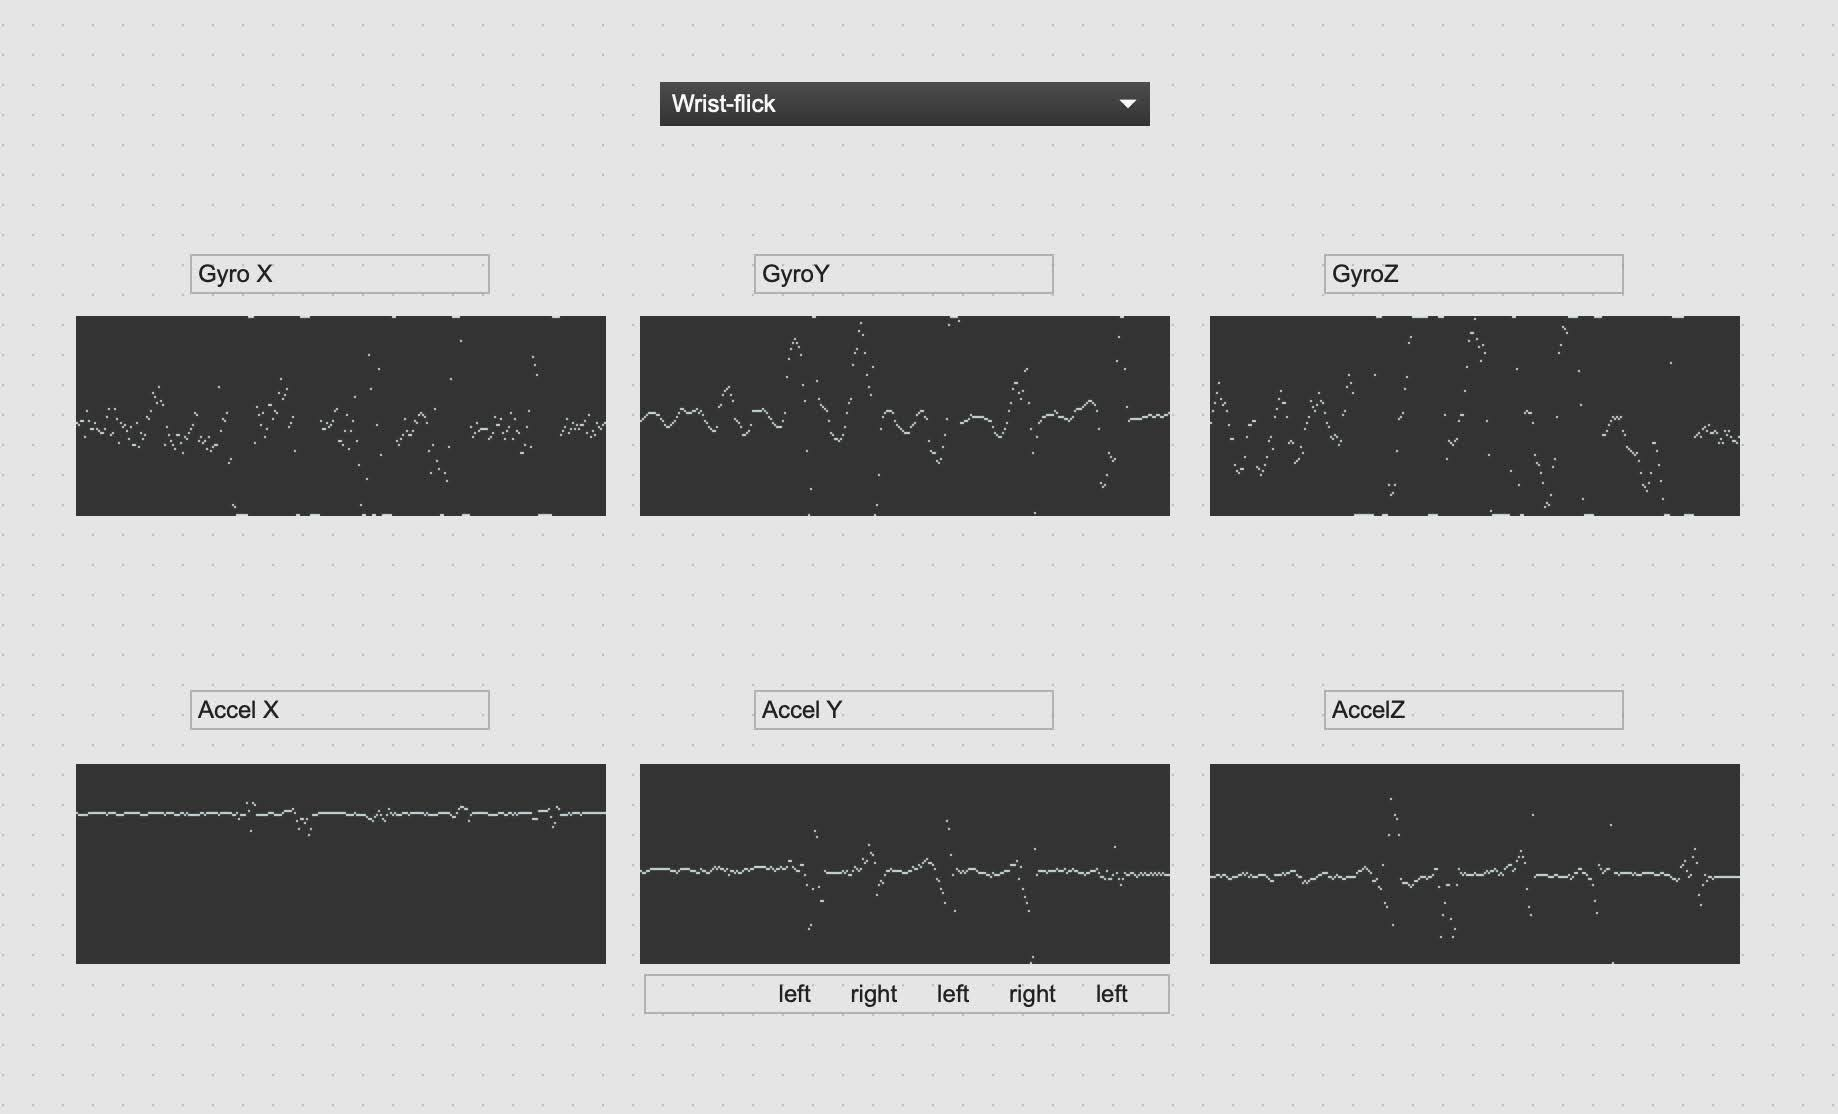
\includegraphics[scale=0.2]{diagrams/gestureData/wristFlick.png}
    \caption{Flicking the wrist holding the Cyberinet.}
    \label{fig:cflick}
\end{figure}


While experimenting with gestures, it is helpful to categorize them in various ways in order to effectively utilize them. To do this, a handful of characteristics are needed.

First, the physical movement should be analyzed. Is it fast or slow? Is it a traditional movement or experimental? What direction is the gesture moving? 

\subsection{Feedback Mechanisms}
In terms of feedback mechanisms, this proved difficult to determine in initial planning and prototyping. Ultimately, two main methods were determined to be useful for both the performer and someone working in the Max environment, without distracting the performer. On the physical unit are multiple LED's. Several of these are used to indicate that the sensors are receiving power, but one LED can be programmed when creating the Cyberinet. 

At the moment, version 1.3 of the software is utilizing the programmable LED to indicate when the sensor data transmits to the computer. This proves useful for determining whether a connection with the computer is established, and if data should be expected by the computer. In order to avoid blinding the user with LED's they are hidden behind the hardware case of the Cyberinet, and small holes are included to allow for intentional inspection.\footnote{Similarly to the metal grates on microwave doors to allow the user to look in on the food while avoiding the microwave radiation.} This programmable LED is located close to the airflow sensor's tubes, allowing for the tube to also function as a light tube to be easily read without needing close internal inspection through the aforementioned holes.

\begin{figure}
    \centering
    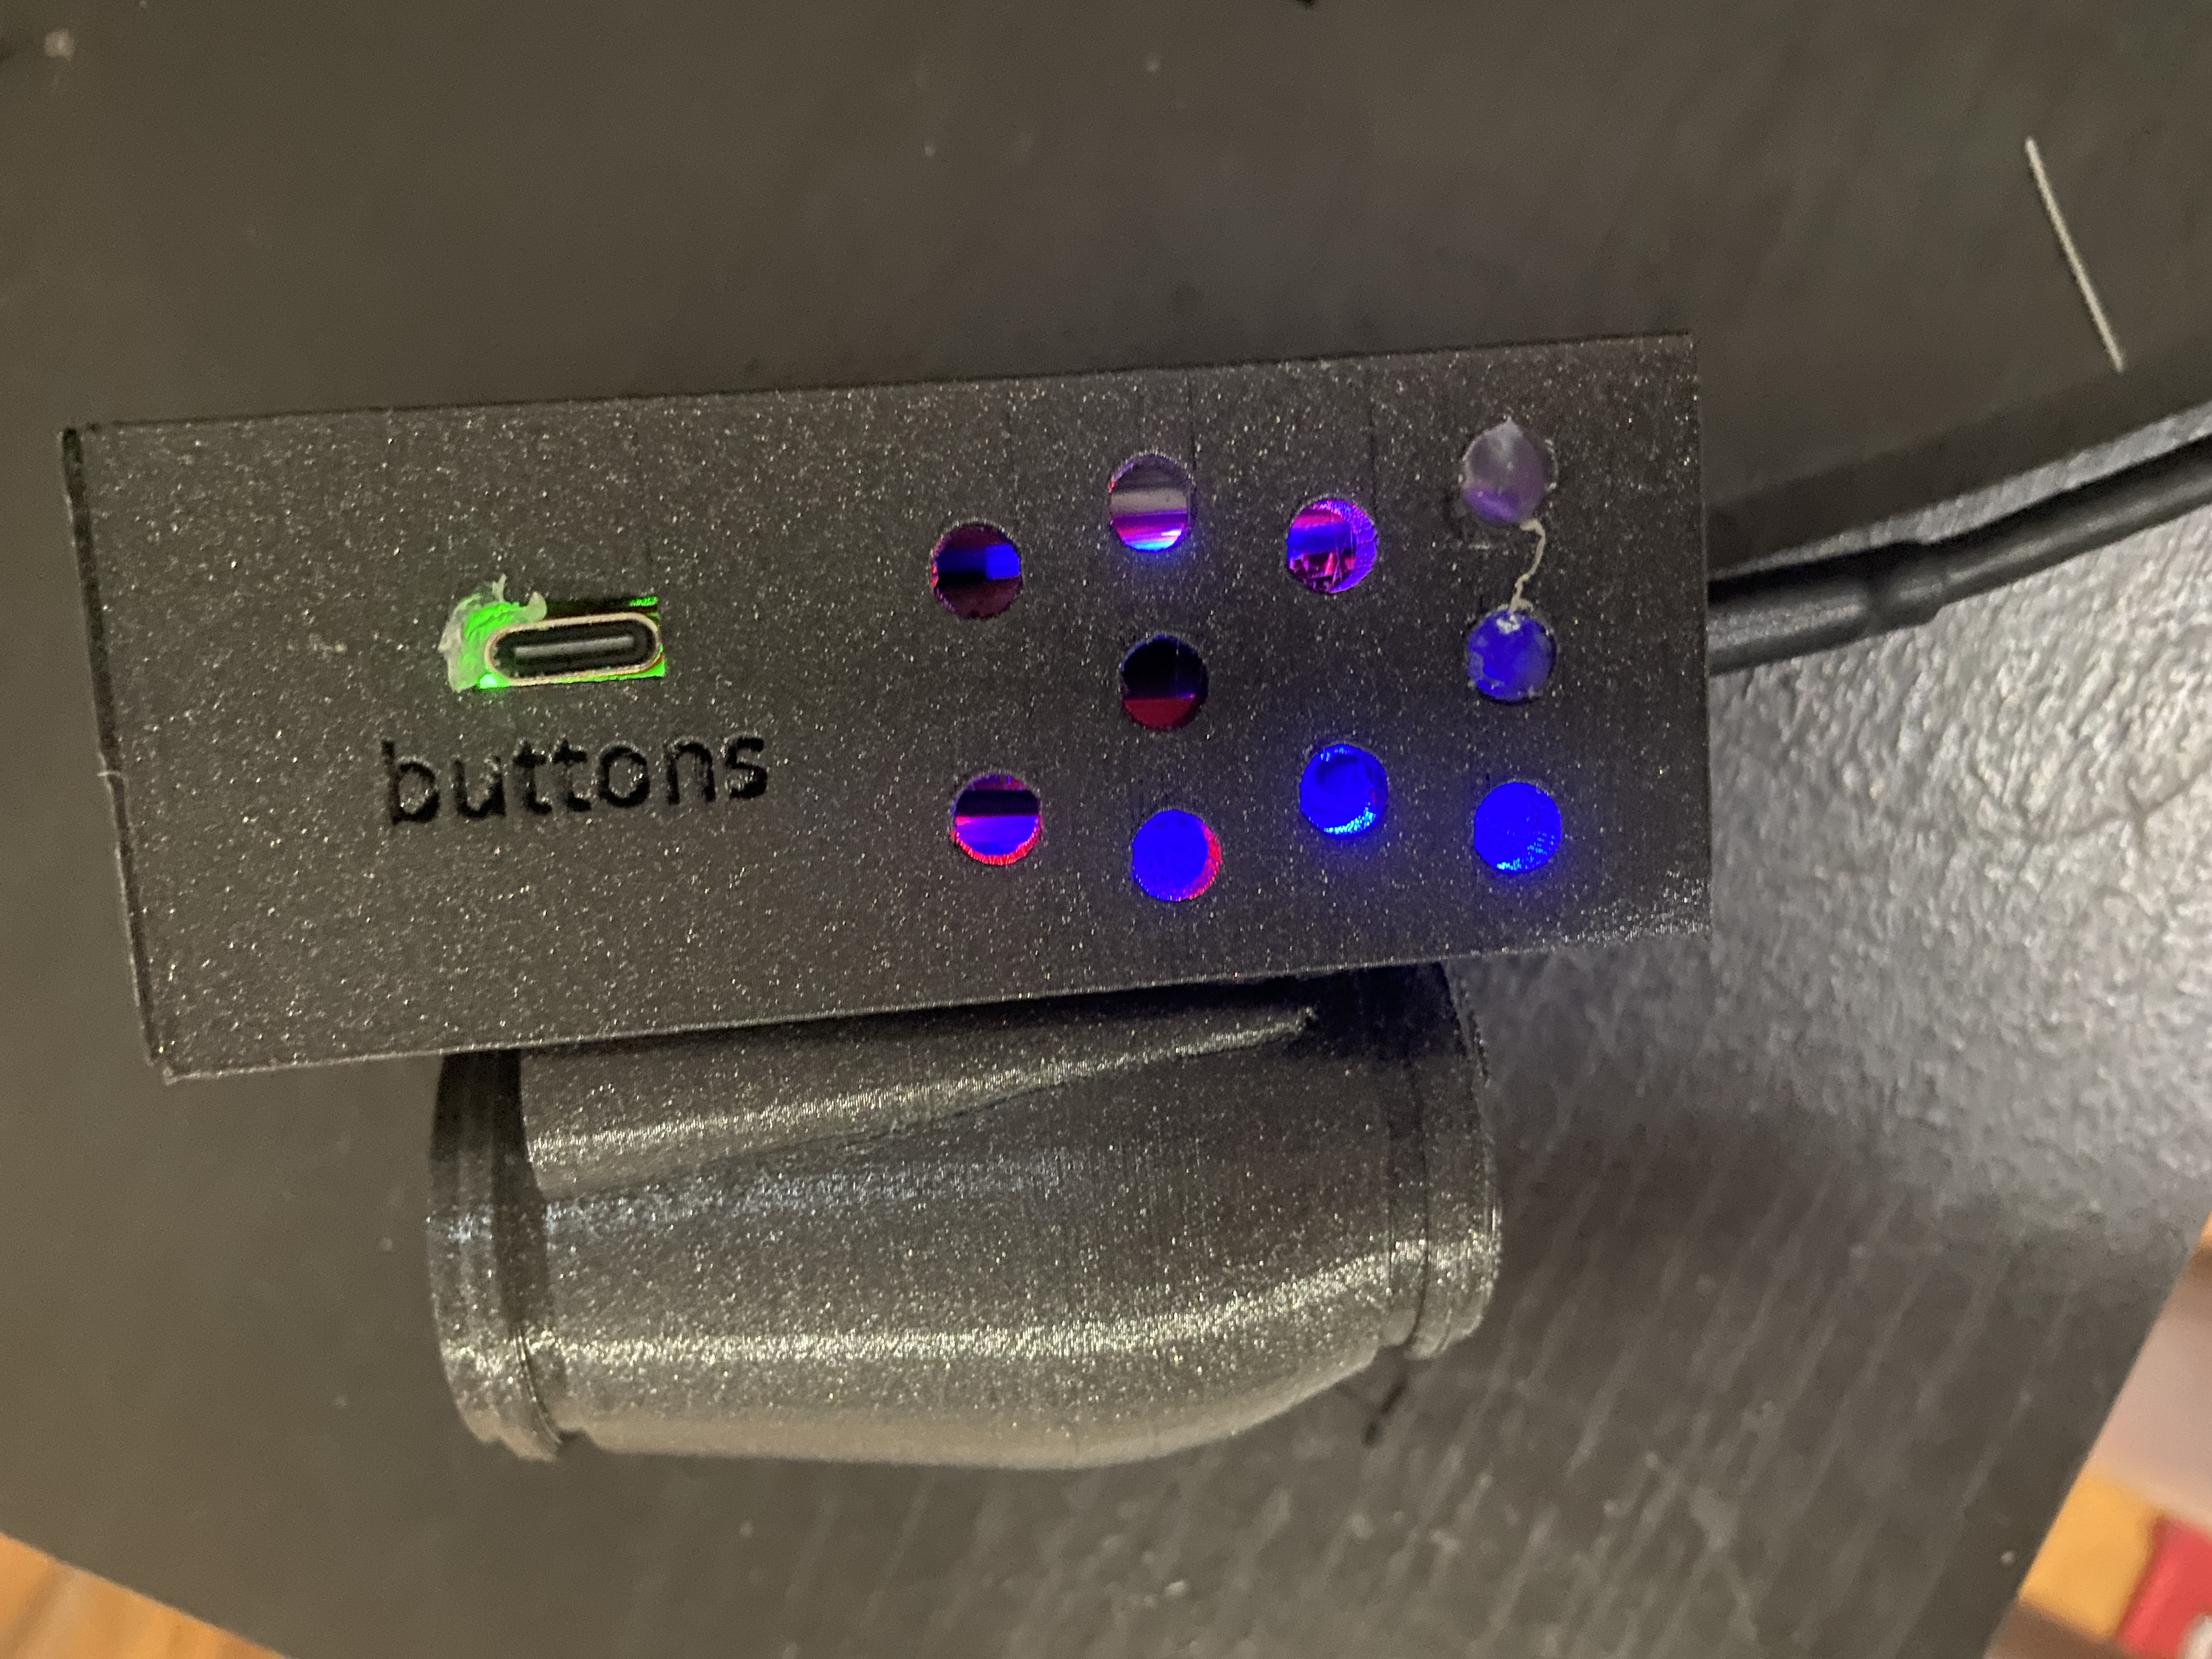
\includegraphics[scale=0.05]{diagrams/IMG_2210.JPG}
    \caption{Power/charging indicator LEDs on the Cyberinet main unit.}
    \label{fig:cyberinetLEDs}
\end{figure}

\begin{figure}
    \centering
    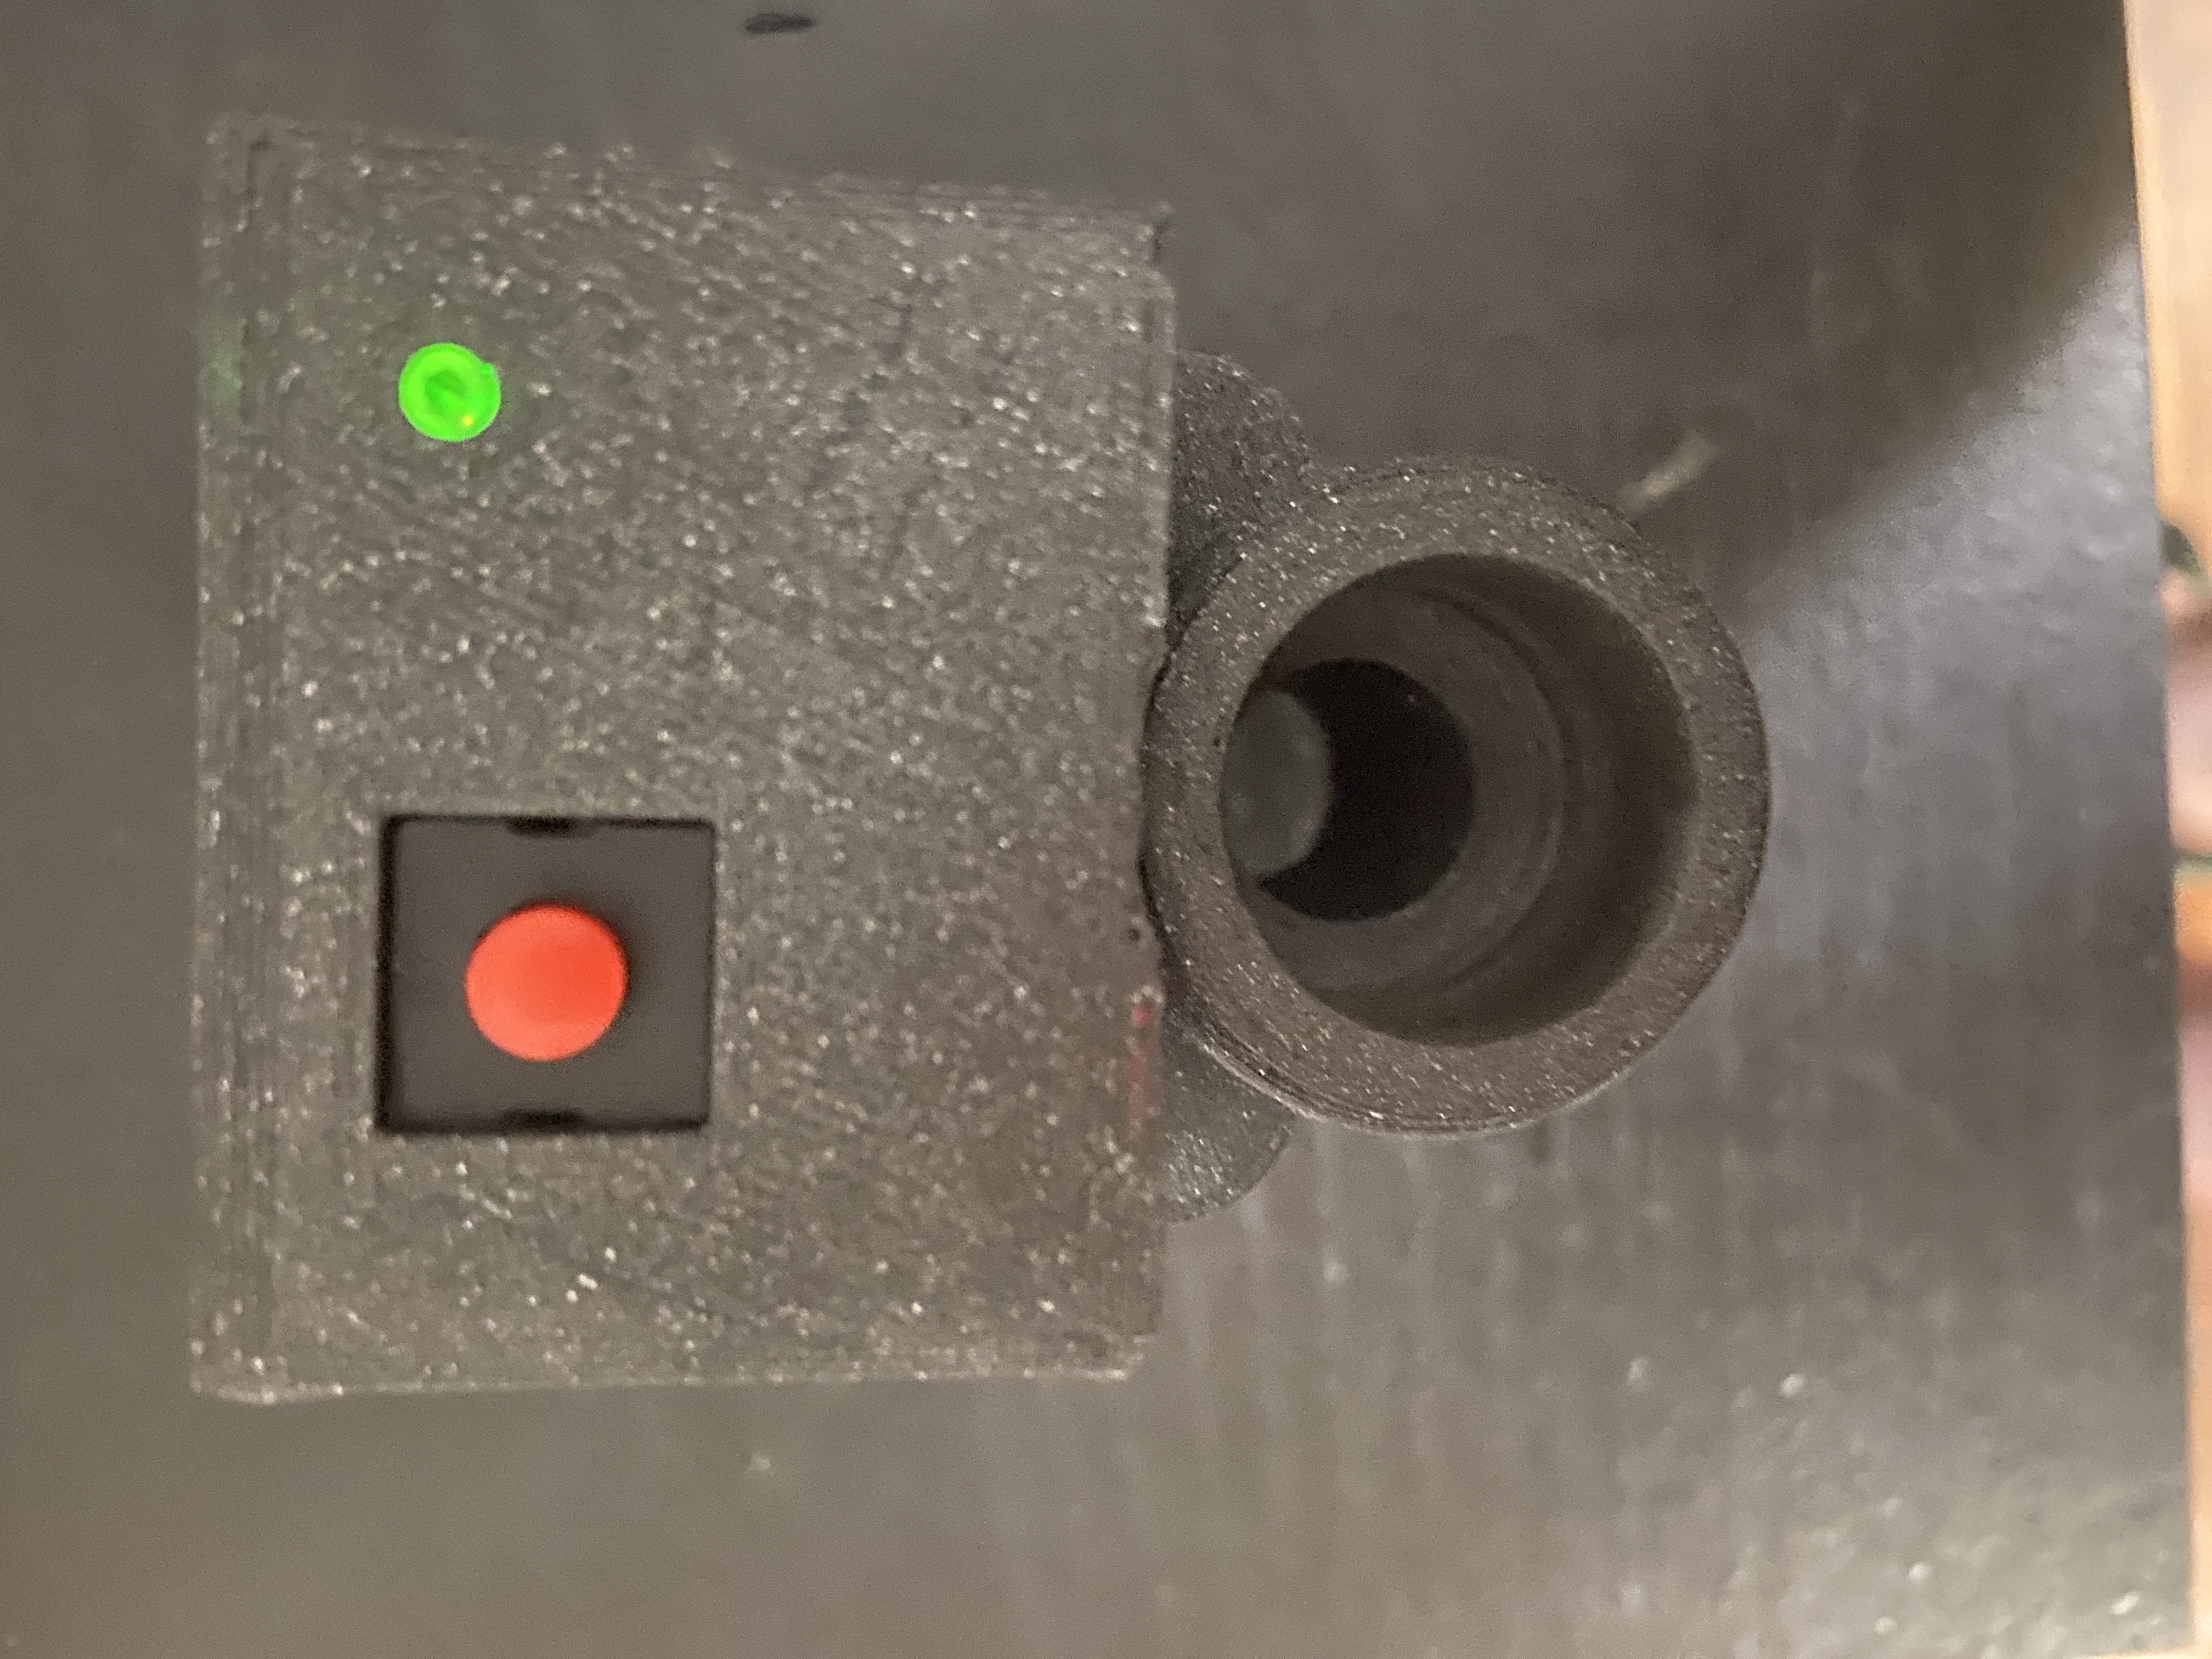
\includegraphics[scale=0.05]{diagrams/IMG_2211.JPG}
    \caption{Toggleable LED visible to the performer while performing.}
    \label{fig:msgLED}
\end{figure}


In the software, a handful of options are available to see the incoming data and any errors. If an unrecognized sensor reading or control message is received by the core CNET software object, this is returned to the user via both the final outlet of the object, as well as the Max console. Because a user would have to go out of there way to include monitoring within the patch, the main Cyberinet patches able to display all incoming data in the same Max console, as well as indicate when communication begins and ends. This is useful for monitoring and recording the incoming data, however at times this can be moving to fast to utilize in real time. Because of this, future versions of the software plan to analyze the data and output more helpful notifications such as unexpected data jumps or noise, signal drops, or abnormal ranges of data.

\subsection{Sound Synthesis} % more here? all of the objects that work with audio are not generating it, just using incoming signal as the processee to their processors.

The Cyberinet is intended to be able to control a variety of software synthesis and control parameters; it does not directly generate sound outside of those produced by the base Clarinet. Because of this, the software is intended to take the sensor data, represent it as a number, then utilize those numbers within the Max programming environment. A handful of Max objects have been created to help facilitate this feature, and for new users to quickly implement the Cyberinet without the need for the user to be an expert in Digital Signal Processing (DSP) and audio effect programming.

All of these effects are built in Max and utilize common control parameters. With the exception of any signal input, receive control messages as floating point numbers between 0 and 1. If the user would like their physical gestures to generate a sound, the sound production must be programmed within Max.

\section{OEM Components}

OEM products are designed to generally compatible with each other. The acronym stands for Original Equipment Manufacturer, and these manufacturers create parts that can be utilized in a variety of different products due to said compatibility. In the case of the Cyberinet, all of the components utilize standardized 0.1in spacing between each pin as well as a common voltage to power the sensor at 3.3V. Every part in the Cyberinet is compatible with these OEM standards, and this is the key to the future expansion units.

While testing various OEM sensors and their capabilities in a performance setting, a series of prototype boards were developed. Early prototyping were done on a bread board in order to test specific uses of pins on the micro-controller and combinations of different sensors. The second step involved creating a hand-soldered board using sockets to be able to easily add or remove components. Once the desired pins and sensors were determined, the socket boards were translated into a more condensed PCB. These were initially created with sockets to allow for more testing and prototyping for future revisions. Once the final design was decided, components were directly soldered to the PCB for formal data capture testing and performance use.

The choice to utilize OEM sensors for the seminal version of the Cyberinet arose both from the outlined method of prototyping, and in order to keep the overall cost down. One of the main design intentions of the Cyberinet was a relatively affordable price point. 

\begin{figure}
    \centering
    \includegraphics[scale=0.55]{diagrams/builtUnits/protos.png}
    \caption{Early prototype socket boards}
    \label{fig:protoBoard}
\end{figure}



\subsection{Micro-Controller \& Power Distribution}

The Cyberinet contains a variety of useful sensors, however without the micro-controller, they become effectively useless in this context. In order to effectively manage all of the sensors and transmit the data, the Espressif ESP-32 DEVKIT V1 was ultimately selected for use with the Cyberinet. This board was selected for a handful of reasons, including:

\begin{itemize}
    \item Board's narrow size
    \item Large number of ports
    \item Arduino compatibility
    \item Wireless communications
\end{itemize}

The first two items on the list are closely related. While being narrower that comparable Arduino units such as the Uno, the ESP-32 DEVKIT V1 has 30 unique I/O Pins\footnote{Other versions of the DEVKIT have 36 GPIO pins. \\These boards are incompatible with the PCBs used in the Cyberinet.}. THer are Arduino boards with similar features, but they were either too large or cost prohibitive to the final design. While four pins are dedicated to power distribution and another for the 'enable' functionality (EN) and resetting the board, the remaining pins be utilized for sensors in a variety of ways. All of this potential functionality is compressed to just under three centimeters wide. Because of the semi-modular design of the Cyberinet unit, having a large amount of accessible pins in a smaller unit was considered ideal. The DEVKIT V1 was preferred over the significantly smaller base chip to increase the simplicity of prototyping, repair, and future changes due to its OEM compatibility, and the popularity of the board among the community.

\begin{figure}
    \centering
    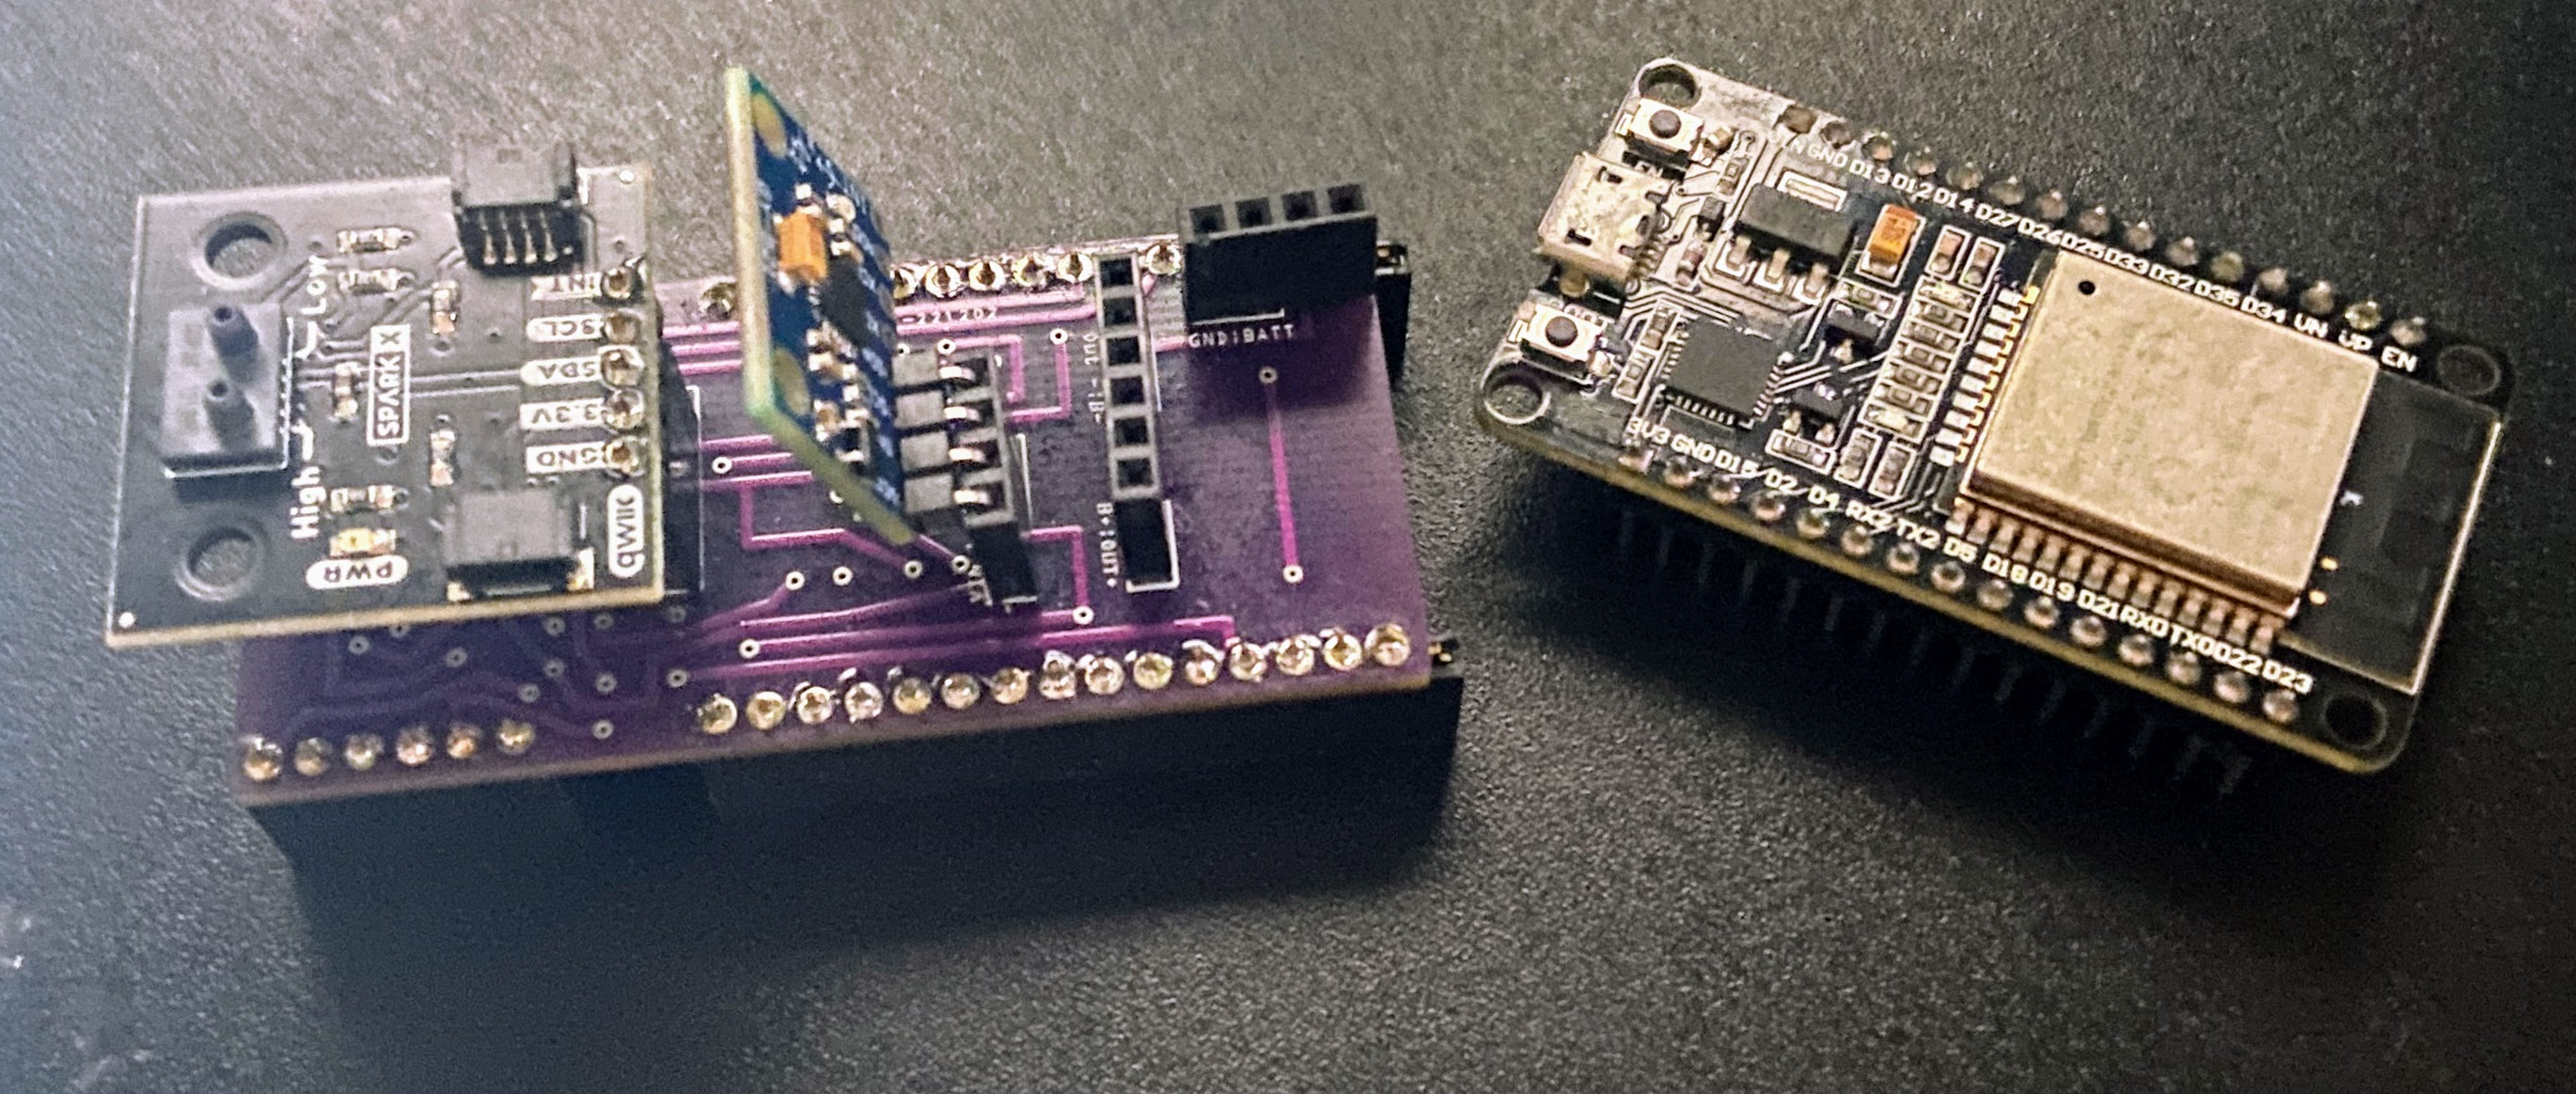
\includegraphics[scale=0.15]{diagrams/builtUnits/protoBoard.JPG}
    \caption{ESP-32 shown next to a prototype PCB. (reprint)}
    \label{fig:protoBoard2.1}
\end{figure}

 

Because of the large number of Pulse-Width-Modulation-Controlled GPIO pins, the Cyberinet has the potential for a large number of sensors and expansions, but to help contain the form factor, only a handful are being utilized at any time. We can see the included sensors attached to the pins as shown below. The labels in the figure below utilizes the pin labels that are printed on the DEKVIT V1.

\begin{table}[]
    \centering
    \begin{tabular}{|c||c|}
    \hline
    Vin     & Power from battery \\
     \hline
    GND     & Ground \\
     \hline
    2       & Power Indicator LED \\
     \hline
    4       & Programmable LED \\
     \hline
    12      & Button 1 \\
     \hline
    14      & Button 2 \\
     \hline
    21      & MPU6050/SDP31 Data \\
     \hline
    22      & MPU6050/SDP11 Clock \\
    \hline
    \end{tabular}
    \caption{Main Unit Core pins}
    \label{tab:mainPins}
\end{table}

The code written for the ESP-32 DEVKIT was created using the Arduino IDE and coding language. For similar reasons to the choice of the DEVKIT, this was done for greater accessibility and simplicity in programming. The board is capable of being programmed in a variety of languages depending on the intended use and the programming abilities of the user. % should I cite a list fo the possible languages, vairants of javascript, c++ python, and a propritaty language by Espressif

The final item from the initial list of board necessities was the wireless capabilities. The ESP-32 is able to perform serial communications with a connected computer via a micro-USB or USB-C cable (depending on the board version). While useful, the goal of the Cyberinet is to provide affordable instrument augmentation with minimal alterations to the clarinetist's performance practice. Towards this goal, minimizing the number of extra cables was a design concern from the first prototypes. By utilizing the ESP-32's built-in Bluetooth capabilities, the performer is able communicate with the computer easily while meeting this requirement.

The ESP-32 also has WiFi connectivity capabilities which may be involved in a future version, but at the current time is currently not utilized. The DEVKIT is able to support Bluetooth version 4.2 and Low Energy protocols for local wireless communication. This allows for the Cyberinet to easily pair with any computer that it has previously connected to using the Bluetooth Serial Arduino library. A code library created by Espressif that brings the normal wired Serial functionality to the Bluetooth functionality of the ESP-32.

While not as powerful as the most up-to-date Bluetooth hardware, the DEVKIT's version 4.2 allows the Cyberinet to connect to a computer from up to 200 feet away with a max data transfer speed of 1 Mbps\cite{btSpecs}. While these values do fluctuate depending on the performance venue layout, and have a minor impedance from the case of the Cyberinet itself, the performance statistics are still high enough for a large majority or performance areas.

\subsubsection{Power Distribution}
In order to power the entire system, a lithium ion polymer battery is included inside the hardware. In order to charge the unit, users can utilize the provided USB-C cable and power adapter to the port located on the bottom of the unit. All power distribution for the Cyberinet is handled with a TP-405 chip, shown in figure \ref{fig:tp5046}. The version containing a USB-C connector was chosen over the Micro-USB connector because of a desire for consistent, modern connectors in the device, which was justified by the board being identical with the exception of the type of port utilized.


\begin{center}
    \begin{figure}
        \centering
        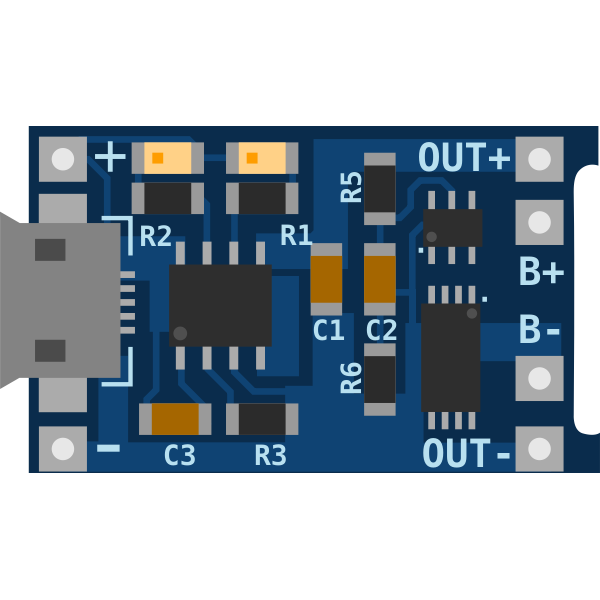
\includegraphics[scale=0.3]{diagrams/1554633962.png}
        \caption{Mock-up of the TP-4056 Power Distribution Chip used in the Cyberinet,\\used by permission}
        \label{fig:tp5046} % public domain svg
    \end{figure}
\end{center}

By connecting the battery to the connections labeled B+ and B-, and connecting the Vin and GND pins of the ESP-32 to the OUT+ and OUT- on this board, the Cyberinet is able to receive all required power through the single chip. The power button is soldered into the connection between the battery and the TP-4056, and will automatically power the Cyberinet when activated. Because of the placement of the power switch, the device will have to be powered on while charging. This can be easily verified by the onboard LED's. 

When the battery is depleted, it must be connected to a power source via this USB-C port to be able to fully charge. From an empty charge, the unit can take between one and three hours to fully charge. The exact times can vary depending on the power adapter and whether any additional accessories are connected. It should be noted that the device can also run when connected directly to the wall socket power supply. This will also charge the battery, which, while resulting in yet another wire, can result in an indefinite run time.

The battery included is rated for 1200 mAh as an improvement over the 320 mAh battery used for initial testing and prototyping. This size battery allows the Cyberinet to have as much run time as possible while still keeping a similar size to the ESP-32, which is the largest OEM component in the Cyberinet. The approximate run times are as follows:

\begin{itemize}
    \item Powered on, not connected: 5 hours.
    \item Powered on, Bluetooth connected, no expansions added: 5-6 hours.
    \item Powered on, Bluetooth connected, expansions added: 4-5 hours.
\end{itemize}



\begin{figure}
    \centering
    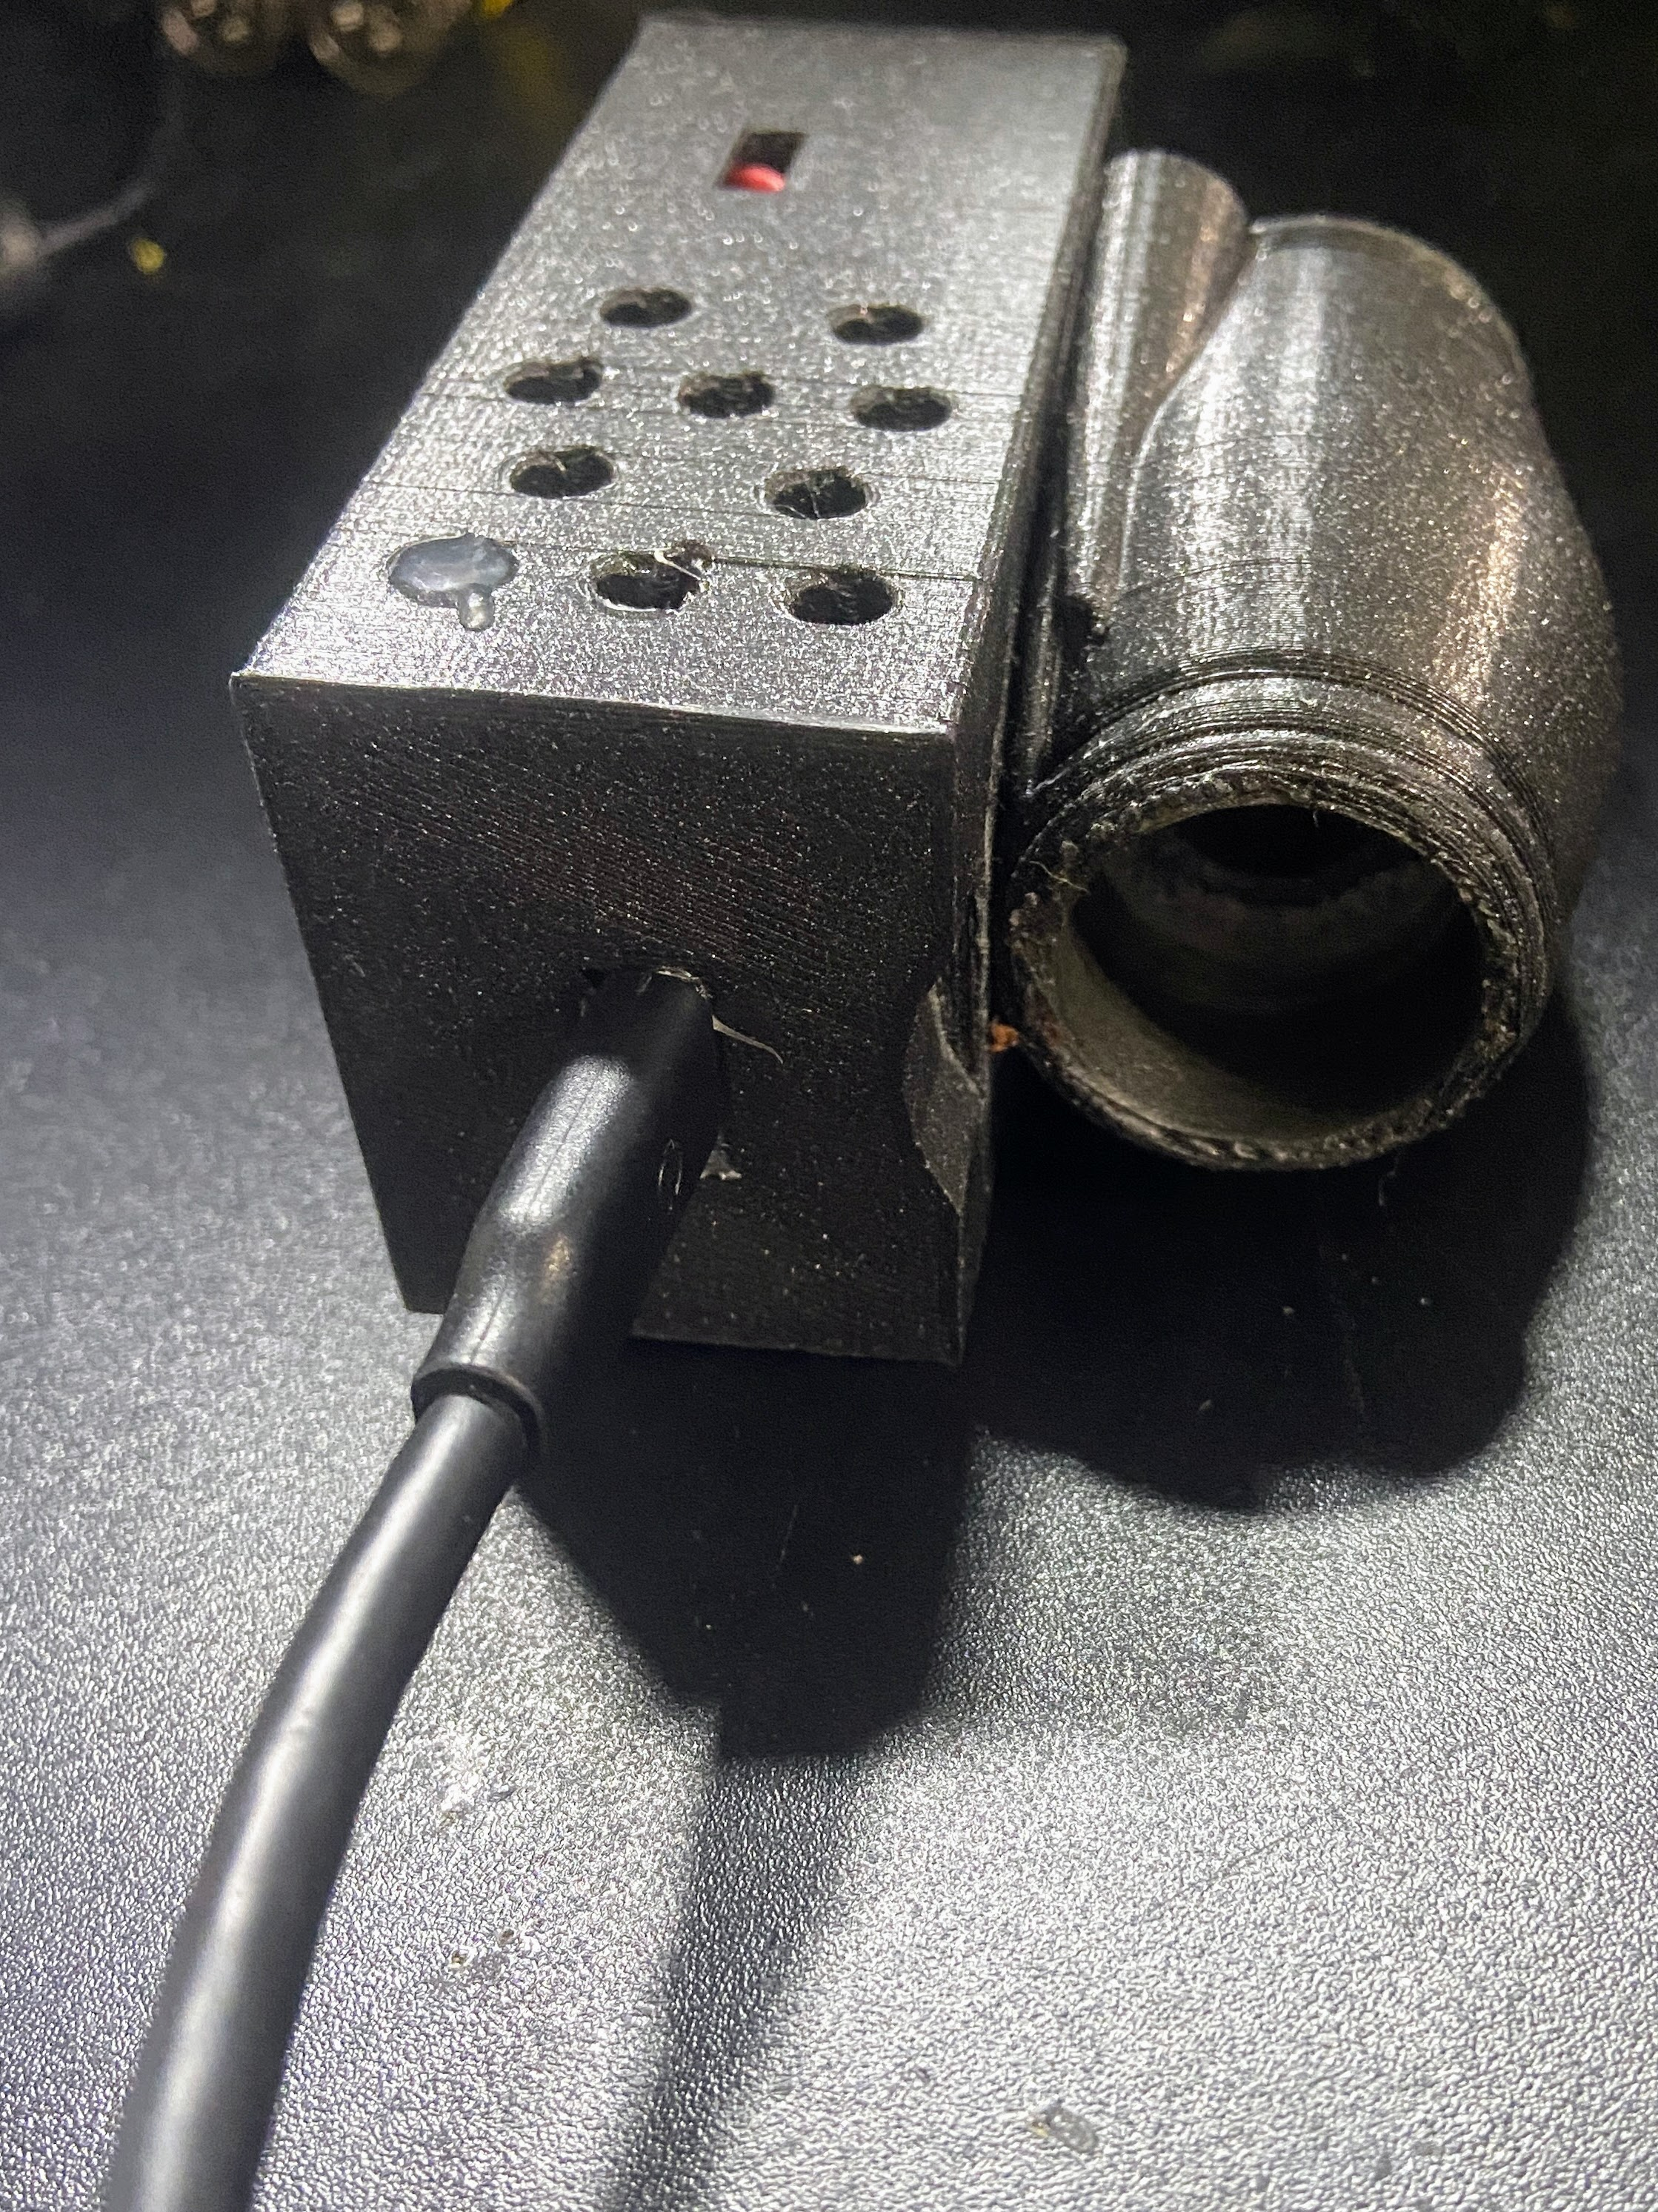
\includegraphics[scale=0.08]{diagrams/IMG_2208 (1).JPG}
    \caption{Charging the Cyberinet}
    \label{fig:chargeUnit}
\end{figure}

\subsection{I2C Sensors}
While all of the sensors discussed in this chapter utilize the same OEM compatibility features, not all sensors are the same. The Gyroscope/Accelerometer, Differential Airflow Pressure, and Thermometer are all I2C sensors, which have their own unique protocol. Due to wire routing constraints, all of the expansion units are intentionally \emph{not} I2C components.

I2C sensors are able to communicate with a host device through their titular data protocol. This is a serial data connection\footnote{a conceptually similar protocol to USB devices connected to a computer.} where both the host device and the attached sensor are able to directly communicate with each other with a syncing clock. While individual sensors may vary, the I2C sensors in the Cyberinet only need the clock and data connections (along with power and ground) in order to function. This helps to reduce the number of traces needed on the PCB, making it easier to design and manufacture.

Looking back to the pins on the ESP-32 micro-controller used in the Cyberinet, only one of each of those pins are present. So how can the two sensors communicate with the controller without the data becoming corrupted? The answer is perhaps the greatest strength of I2C communications. Devices using I2C communicate on specific addresses. This means that multiple sensors can all connect to the same clock and data pins, and each will work as long as they are utilizing unique addresses. Because the address is represented as a 7-bit value, the maximum number of potential I2C devices that can be connected to a single host is 127.


\subsubsection{Gyroscope \& Accelerometer}

The main motion-detecting sensor utilized in the Cyberinet is the MPU-6050. This is a commonplace sensor containing a six degree-of-freedom gyroscope and accelerometer. The board also contains a thermometer, but this one is not utilized. The MPU6050 communicates on I2C address 0x68., but his can be changed to allow for an additional 6050 to connect to the same host.

\begin{center}
    \begin{figure}
        \centering
        \includegraphics[scale=0.3]{diagrams/GY-521_MPU-6050_Module_3_Axis_Gyroscope_+_Accelerometer_0487.jpg}
        \caption{MPU-6050 Gyroscope and Accelerometer}
        \label{fig:6050}
    \end{figure}
\end{center}

Within the IC shown in the center of figure \ref{fig:6050} are the MEMS components for the gyroscope and accelerate. These incredible small components are able to interact with each other and bridge specific connections in order to determine which direction the device is moving, and how quickly that movement occurs\cite{6050HowTo}.


\subsubsection{Differential Airflow Pressure \& Thermometer}

Originally released in 2017, this is the newest hardware component utilized with the Cyberinet. This unit detects differential airflow pressure between two points as well as temperature. Due to the SDP-3X line’s small form factor, the Sparkfun Qwiic connector breakout board was selected for simple, OEM compliant installation. Two small tubes are attached to the ports and used to measure the air pressure difference between the inside of the Cyberinet barrel and the outside of the instrument. This is the same tube as shown in figure \ref{fig:msgLED}.

\begin{center}
    \begin{figure}
        \centering
        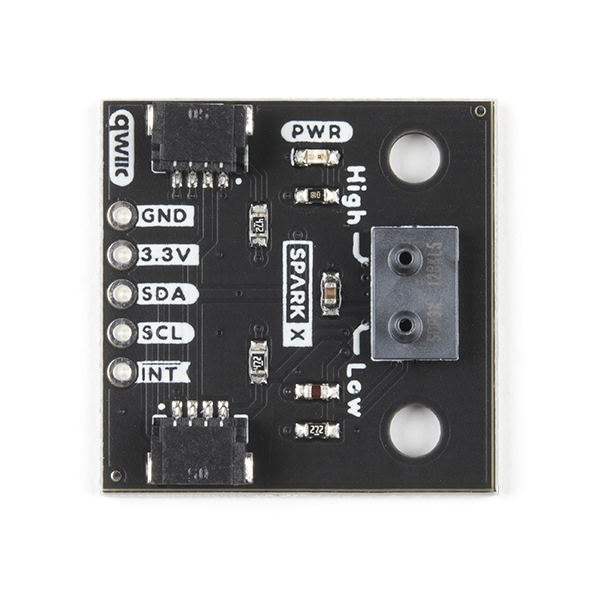
\includegraphics[scale=1.5, angle=90]{diagrams/oem/spd31.jpg}
        \caption{Sparkfun SDP-31 Differential Airflow Pressure Qwiic Connect Breakout Board} %replace with my picture
        \label{fig:sdp-31}
    \end{figure}
\end{center}

A differential pressure sensor functions by placing a diaphragm in between two pressure points. in the SDP-31, this is located in between the two hose attachments. At the pressure between the two areas changes, the diaphragm position will move, and this movement represents the difference in pressure between the two points\cite{airflow}.

Because of it’s higher accuracy, the SDP-31’s temperature sensor is utilized over the MPU-6050. Temperature is measured in degrees Celsius. This sensor utilizes address 0x21 be default. By cutting or bridging pads on the bottom of the breakout board this address can be changed to one of three possible options depending on the specific use case.

\subsection{Optional Expansion Sensors}
In addition to the built-in I2C sensors, the Cyberinet utilizes a variety of optional expansions that can be implemented as needed to customize the array of sensors. The main expansion unit contains two momentary push buttons and is discussed in greater detail below. As previously mentioned, these sensors are \emph{not} I2C sensors, and utilize specific pin combinations without the serial protocol. At the time of writing, one expansion unit has been completed, with plans for two more underway.

\subsubsection{Button Expansion}

\begin{center}
    \begin{figure}
        \centering
        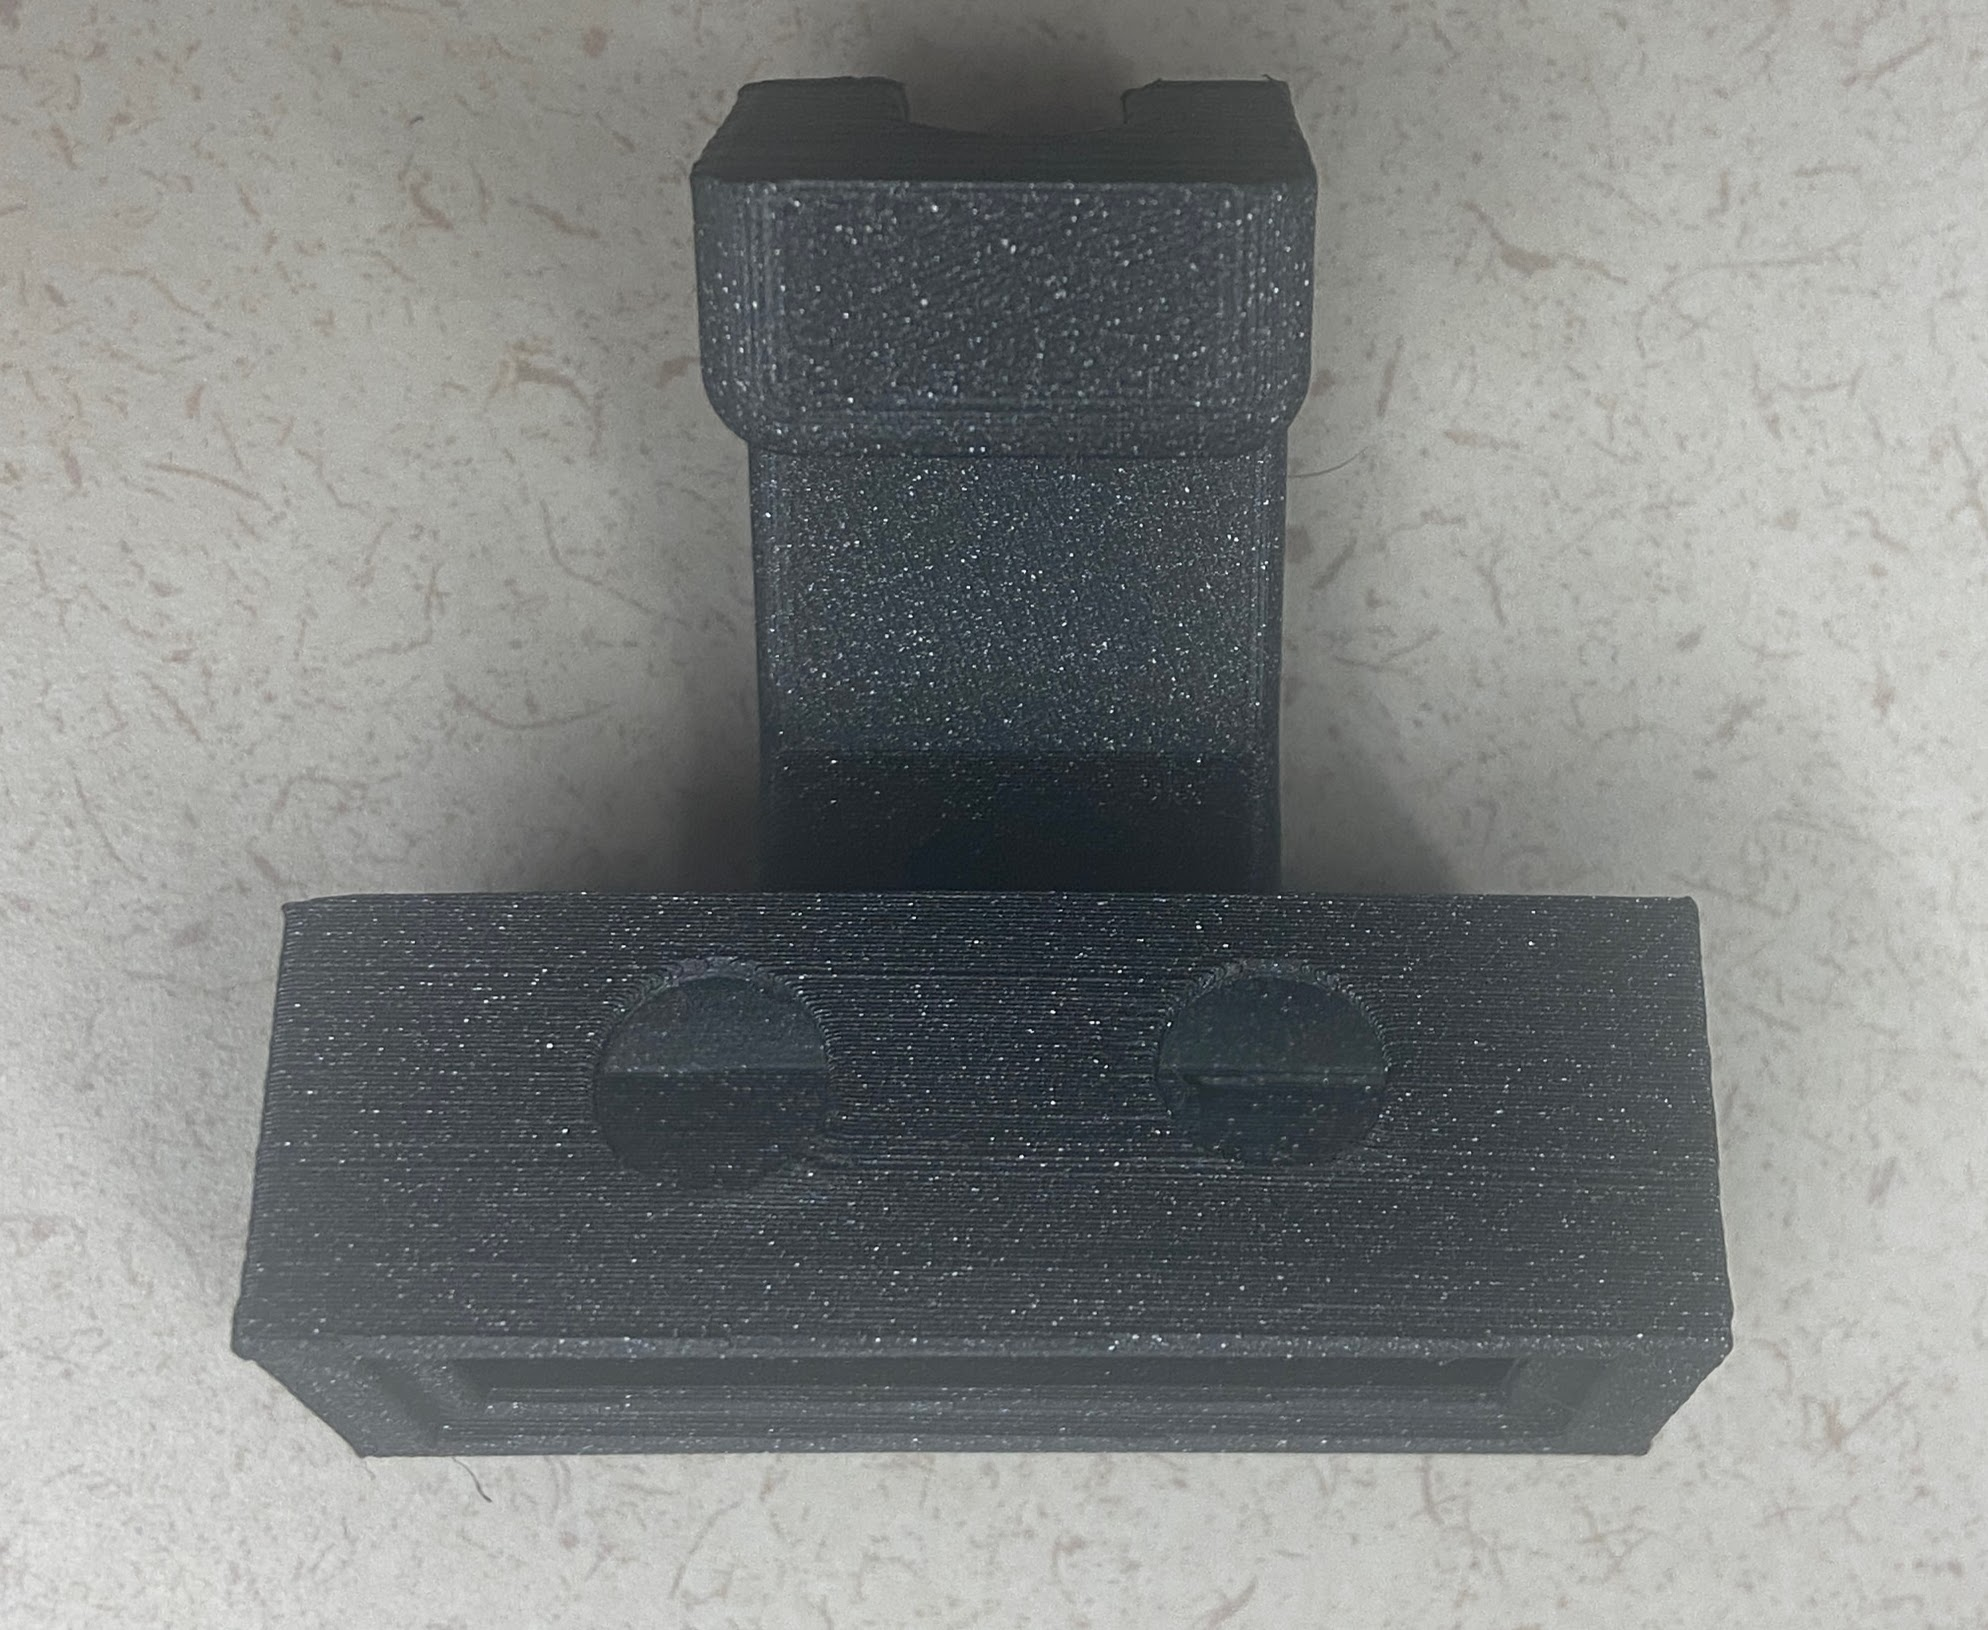
\includegraphics[scale=0.1]{diagrams/builtUnits/buttonhousingEmpty.JPG}
        \caption{Empty 3D-printed thumb rest with housing for buttons below.}
        \label{fig:buttonThumbrest}
    \end{figure}
\end{center}


The Button Expansion is much simpler when compared to the main unit. The unit is composed of only two mechanical buttons with built in LED's, two resistors for those LED's, a USB-C port for communication with the Main Unit, a PCB to route all of the connections and the 3D printed housing. The button expansion is designed to be attached to the performer's thumb rest to allow for easy access with the right thumb. However it is also shaped in a way to allow for it to be held in the hand or placed elsewhere.

To assemble the unit, all components are soldered to the PCB. In a similar manner to the main unit, SMD components are attached first, followed by cables, and finally the larger components, the buttons, last. This process of assembling from smaller-to-larger components is present in all parts of the Cyberinet  The completed PCB is then secured within the 3D-printed housing to complete the unit. The PCB for the Button Expansion is shown in figure \ref{fig:buttonPCB}, and the version of the PCB containing all of the components soldered to it is part of figure \ref{fig:CyberinetNoCase}.


\begin{center}
    \begin{figure}
        \centering
        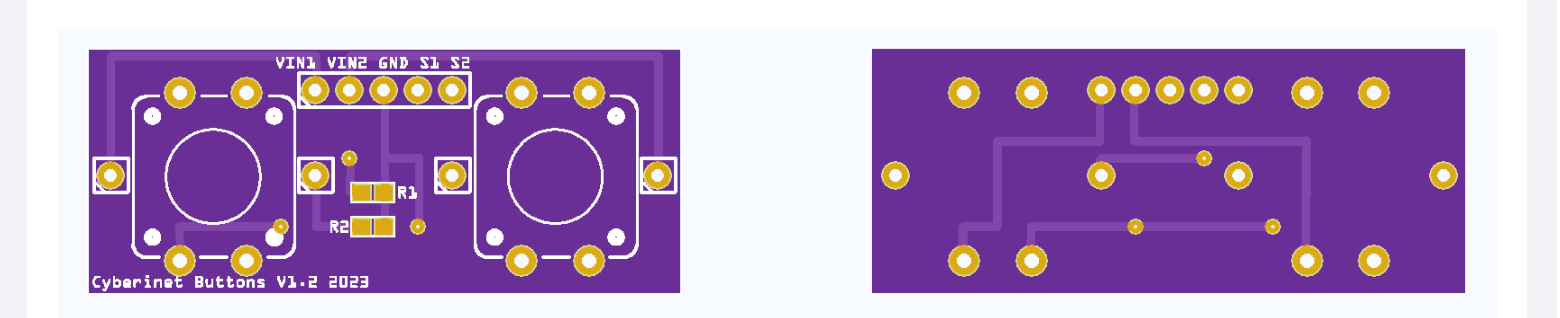
\includegraphics[scale=0.5]{diagrams/PCBs/buttons1.2.png}
        \caption{Button Expansion PCB}
        \label{fig:buttonPCB}
    \end{figure}
\end{center}


Expansion Units are optional and not needed for the Cyberinet main unit to be functional and are intended to only be connected when needed for a particular performance. All the expansions connect utilizing a standard USB-C connector. However, because these units do not utilize the USB protocol, so both the main unit and expansions cannot be connected to a computer via these ports. While a set of USB-C cables that are functional is included with the full Cyberinet set of hardware, The main reason for utilizing this connector is for the end-user to be able to supply their own cables of various lengths depending on their needs. 


\begin{center}
    \begin{figure}
        \centering
        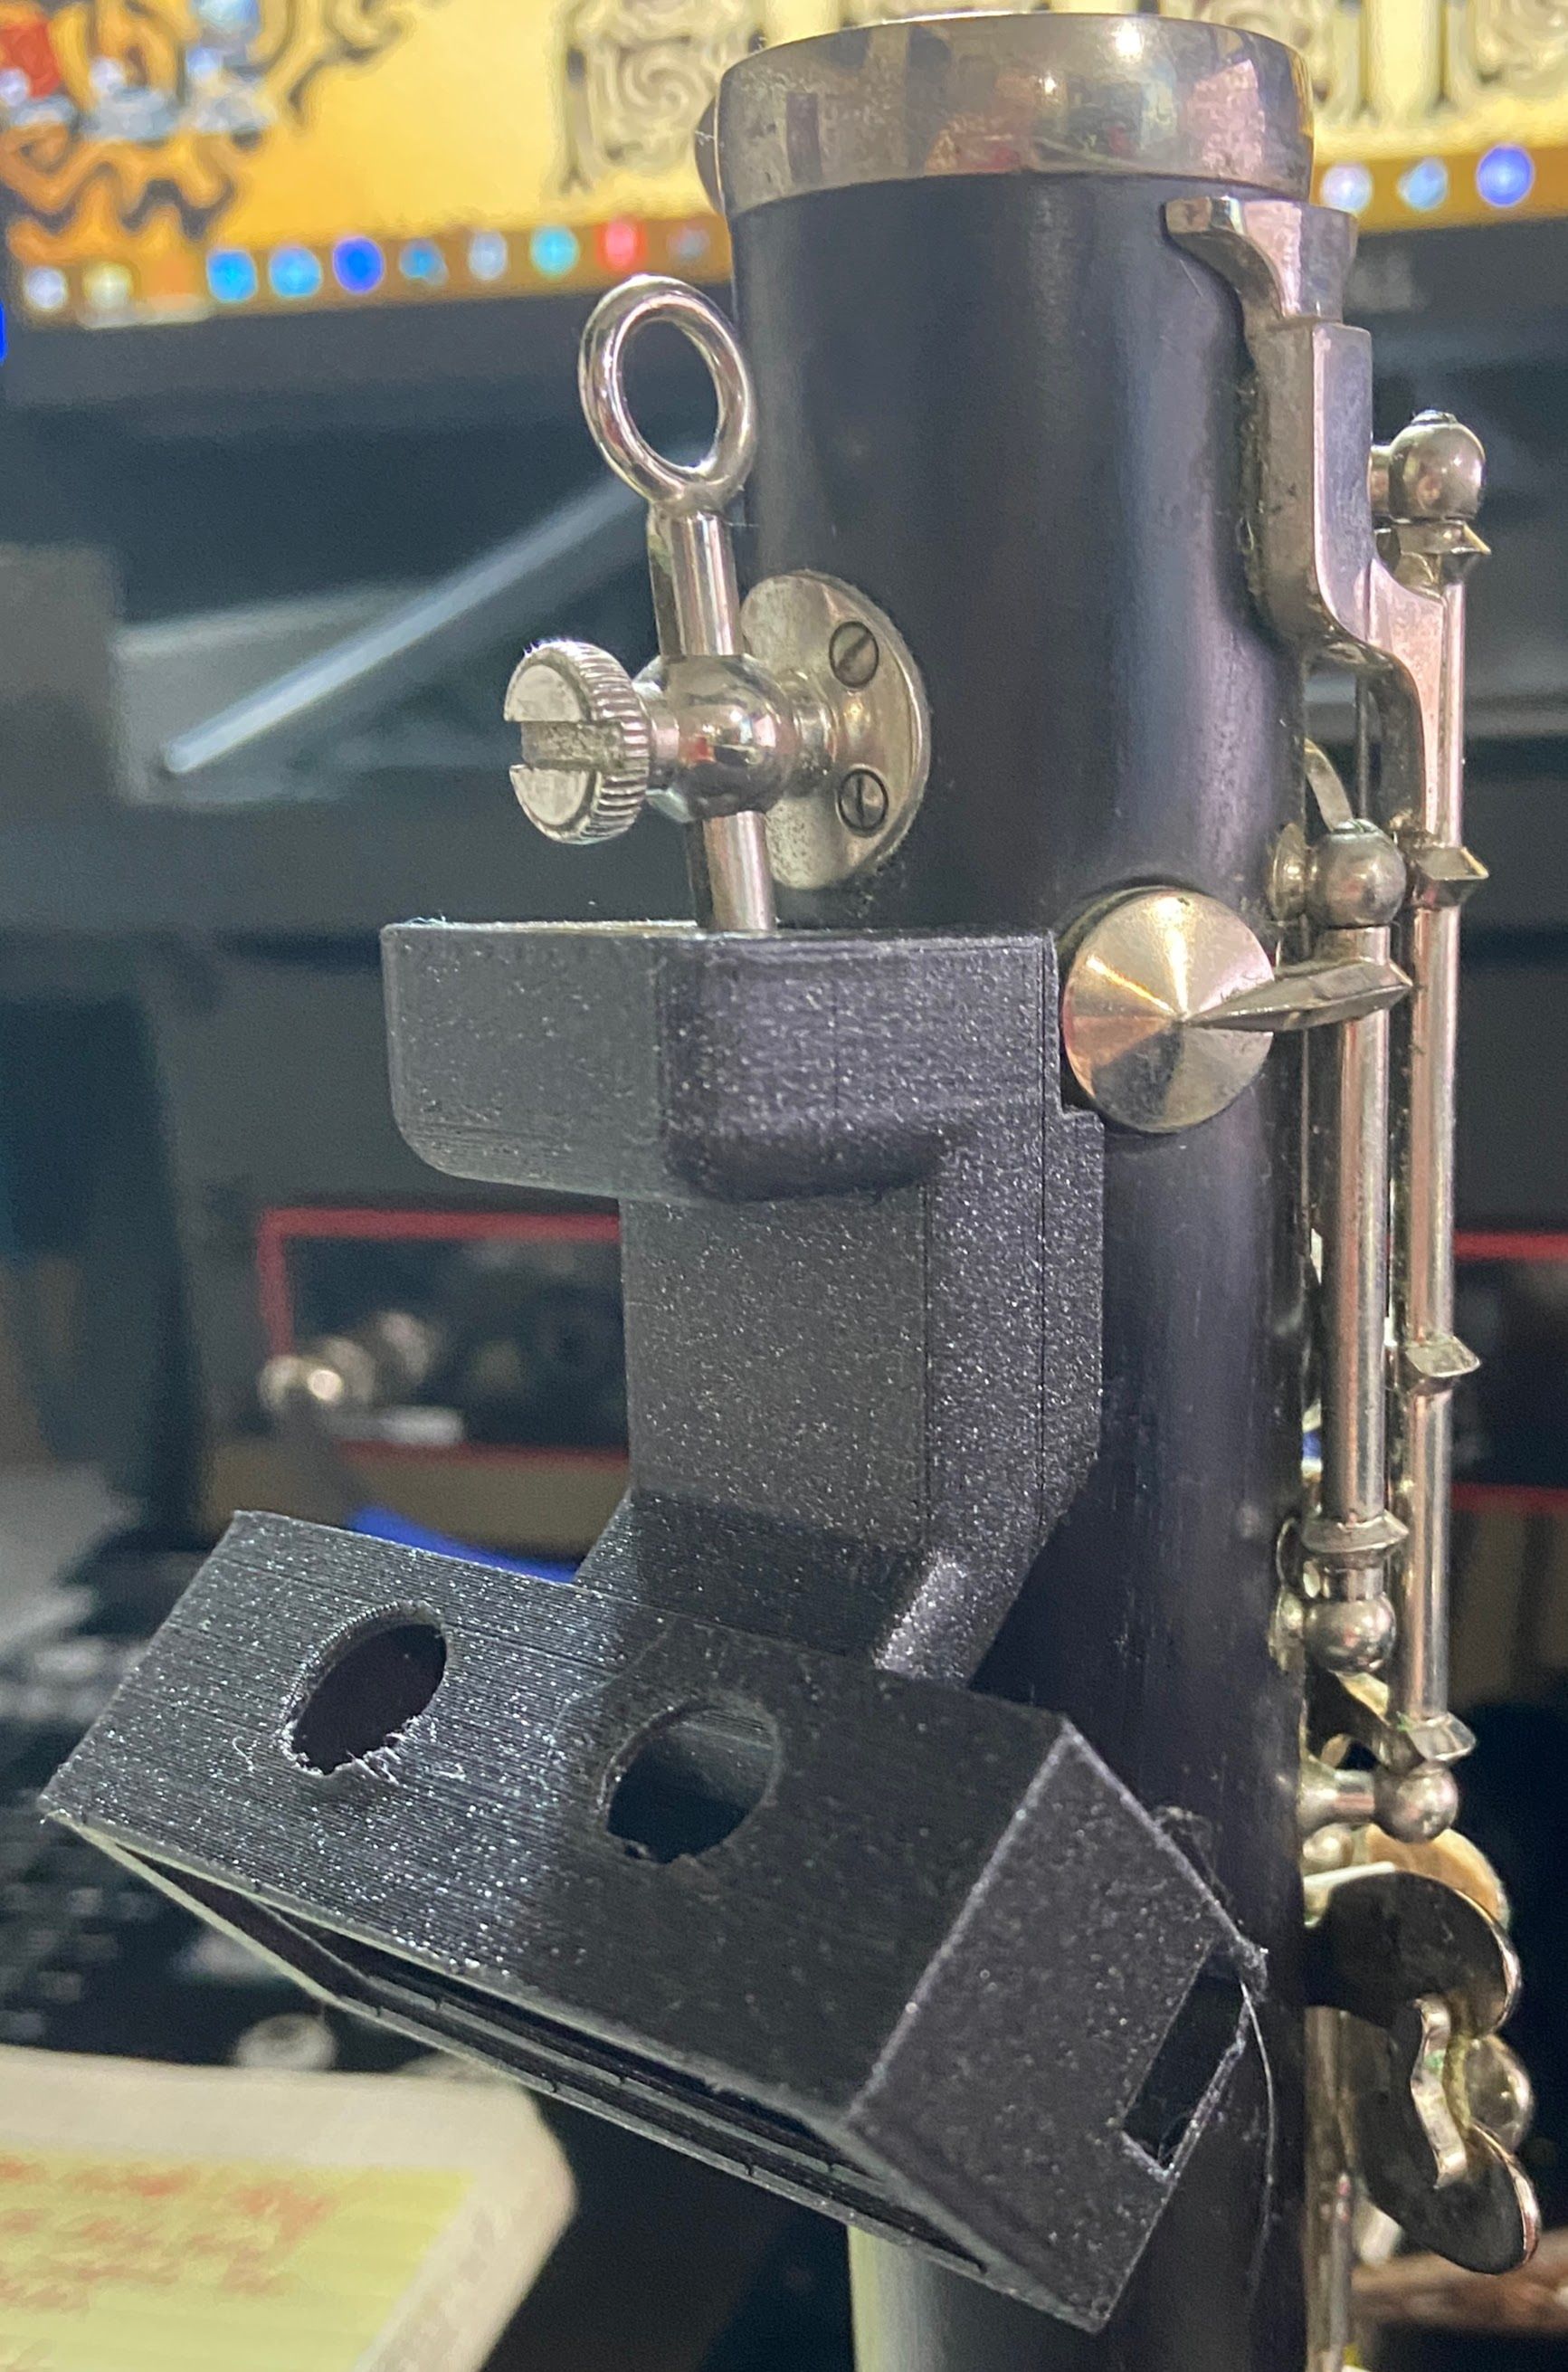
\includegraphics[scale=0.08]{diagrams/builtUnits/thumbOnInst.JPG}
        \caption{Empty Button Expansion placed on a Clarinet thumb rest}
        \label{fig:thumbOnCase}
    \end{figure}
\end{center}

This expansion, while optional, is incredibly useful for a performer on stage. They can access the buttons using their right thumb when performing. This maneuver is easier when utilizing a neck strap, so the performer can place the buttons elsewhere if they like using a longer connector cable. The closeness between the buttons and thumb rest is shown in figures \ref{fig:buttonThumbrest} and \ref{fig:thumbOnCase}\footnote{The case has been revised since the initial picture was taken. The small rectangular hole for the connection cable has been moved to the left side to avoid potential collisions with the performer's hand.}. Each button also contains a single, colored LED built into it to provide feedback to the performer. By default, the lights are only illuminated when the button is pressed. The Cyberinet simply detects whether a button has been pressed and transmits that data as a Boolean value to the computer. Using Max, the user can have the buttons achieve functions from near limitless hypothetical list of options. For this project, the buttons were used to trigger microphone recording and buffer playback, however objects that take the button input and move between various presets, trigger DSP, and turn pages of a score have also been developed and included in the software bundle for this project.

\begin{figure} %crop image if I have time
    \centering 
    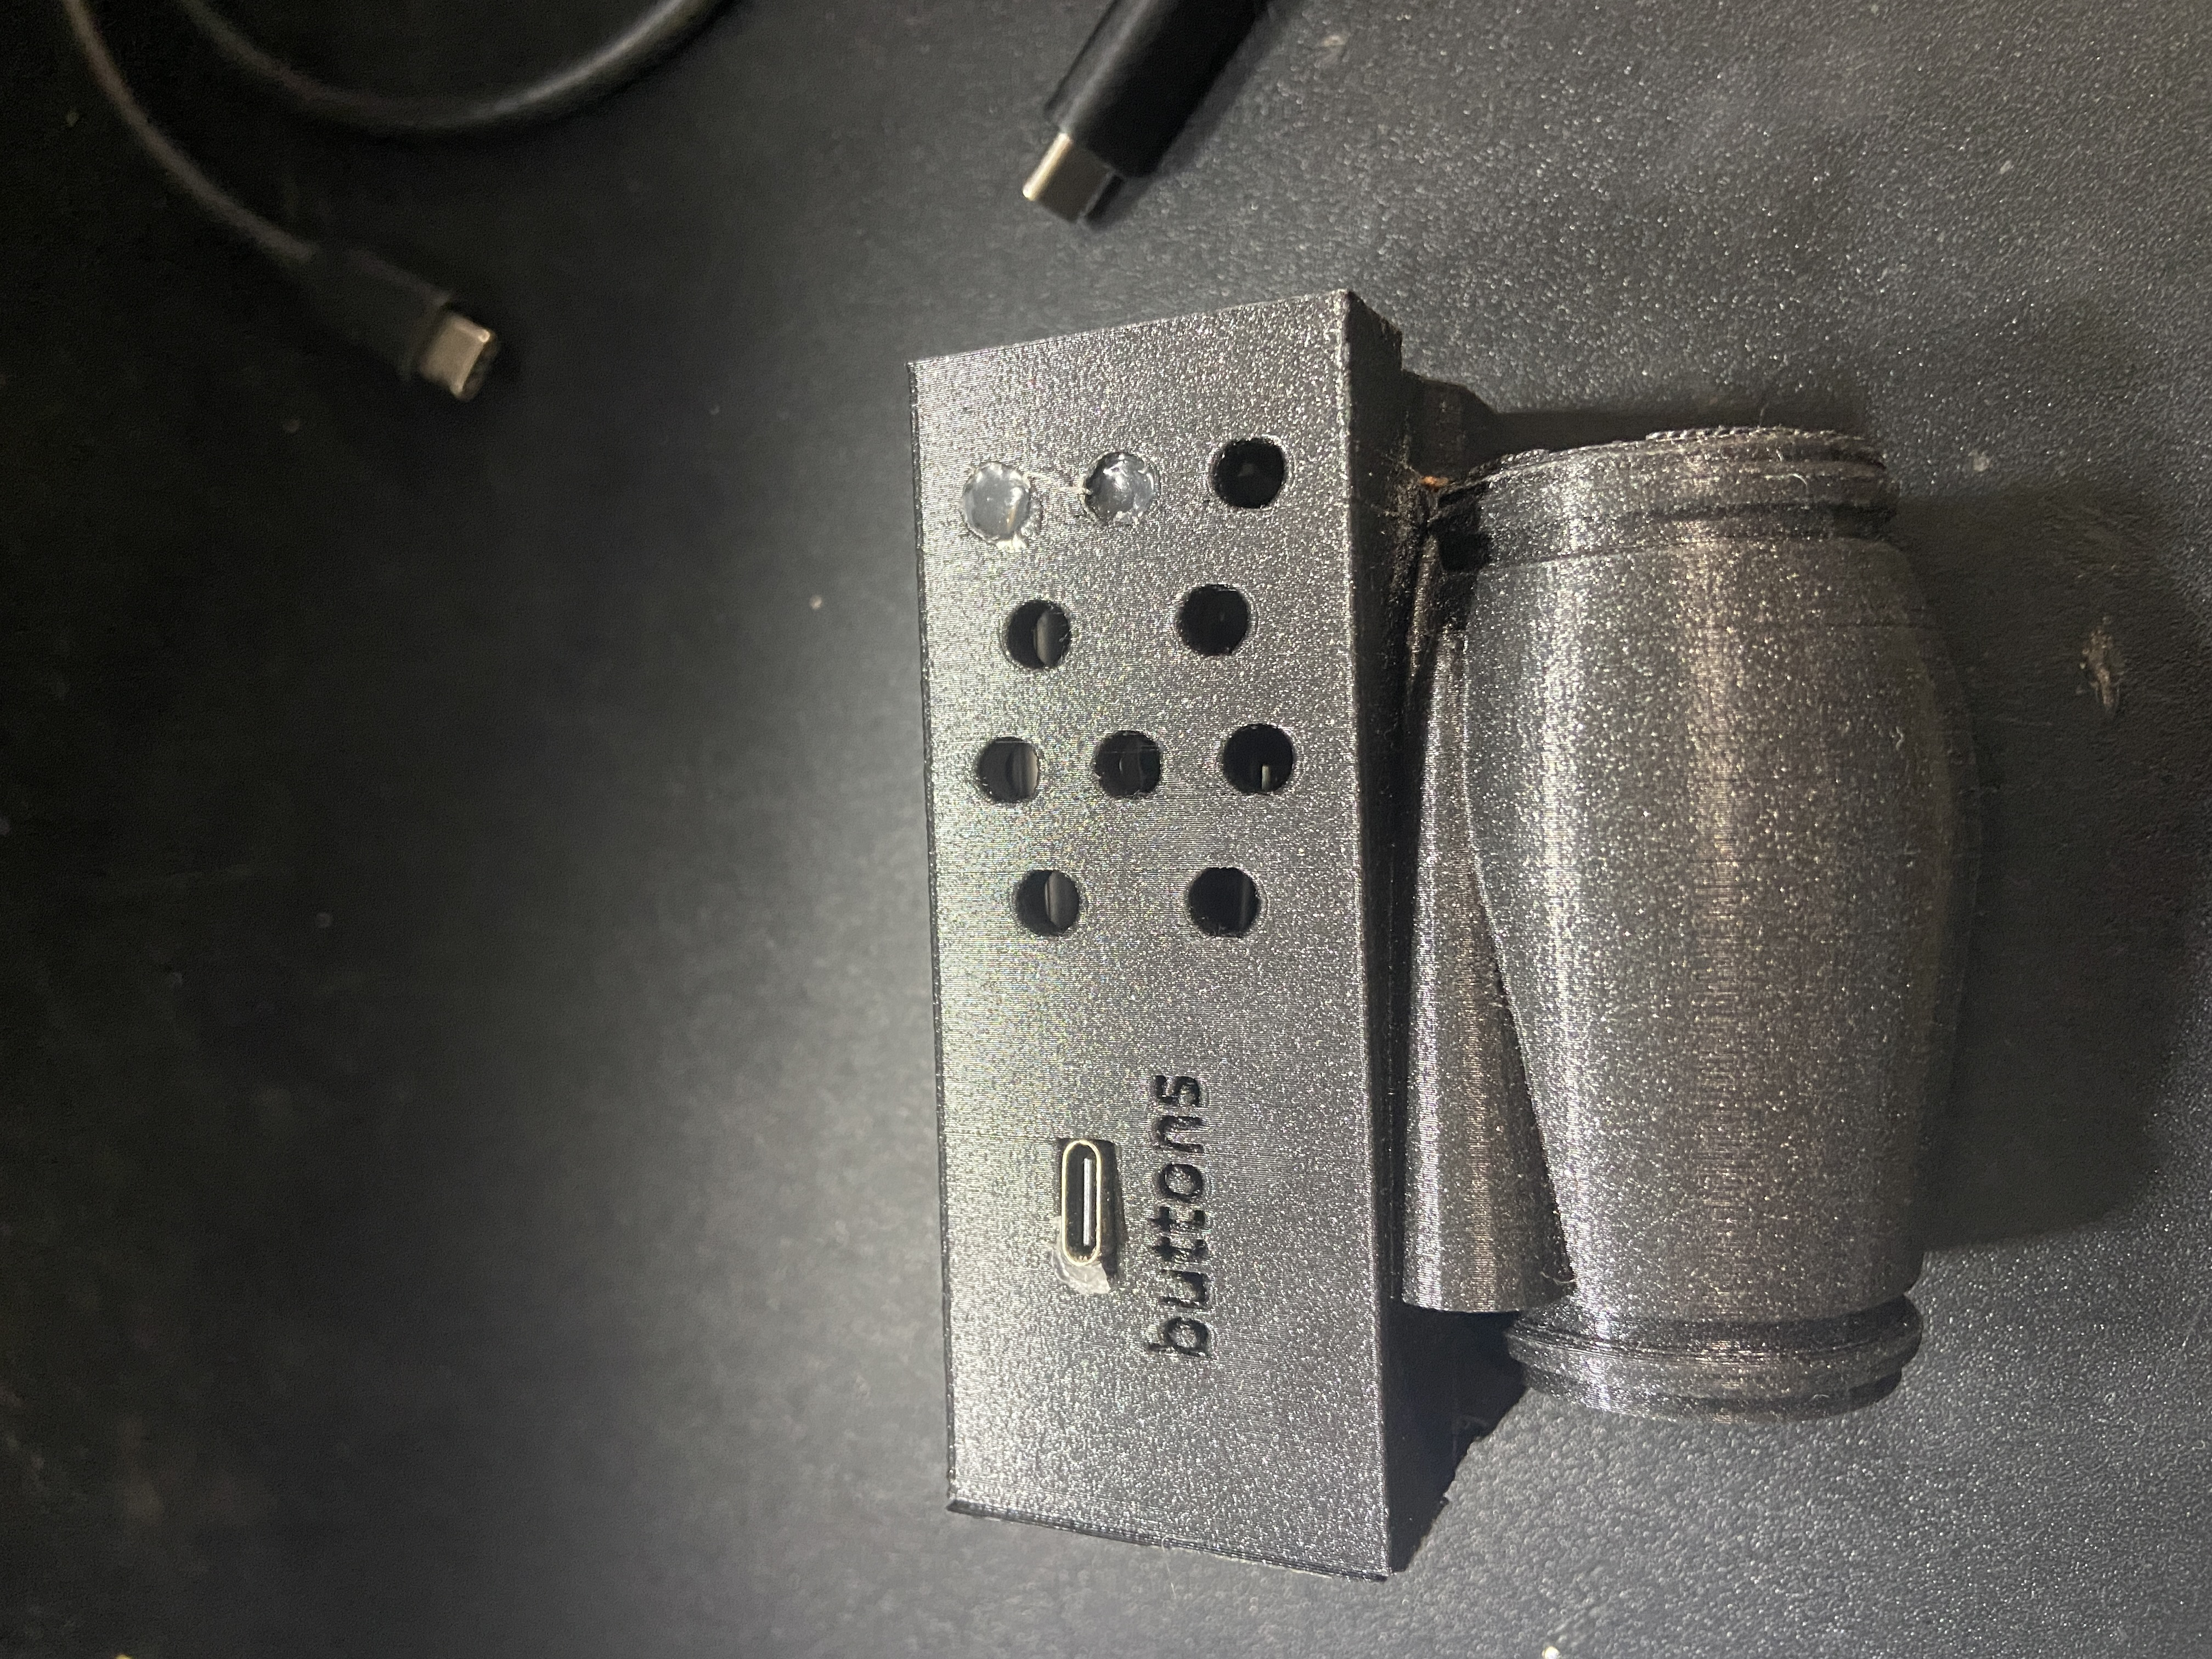
\includegraphics[scale=0.05, angle=270]{diagrams/builtUnits/buttonPort.JPG}
    \caption{Location of the Button Expansion port on the Cyberinet.}
    \label{fig:buttonPort}
\end{figure}

The port for the buttons is located on the upper portion of the Cyberinet main unit in order to reduce the amount of wire needed to reach the PCB, as well as to visually distinguish it from the charging port. Because a differing number of pins is used between this and the other expansion port, located in the same location on the opposite side of the unit, is given the label "buttons". The main unit can be rotated 360 degrees in order to adjust the positioning of the button expansion cable to wherever the performer desires.

\subsubsection{Other Expansions}
At the time of writing, only the button expansion has been developed and tested completely. However, in-progress plans for a continuing range of expansions exist.

The joystick expansion is relatively simple. It is designed to receive data from the single button and two potentiometers of a standard joystick. The PCB diagram shown in figure \ref{fig:jsPCB} shows the simplicity of this setup.Power and ground are received and fed to both the joystick as well as the power indicator LED. The values from the horizontal position, vertical position, and button are all returned to the ESP-32 on pins 33, 32, and 35 respectively. When transmitting to the computer, the data receives the labels exp1, exp2, exp3, and exp4. All expansion units receive the same labels with a different number because they are interchangeable. This removes the need for a the unit to have to identify the expansion and apply the appropriate label. The number specifies the specific pin that the data is receiving, and the connectors of the physical units are wired to consistently begin with exp1 and utilize up to the four available pins.

\begin{figure}
    \centering
    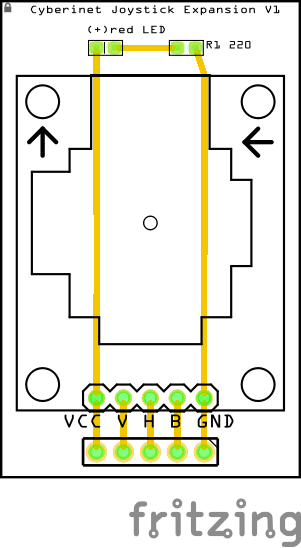
\includegraphics{diagrams/PCBs/thumbPCBv1.png}
    \caption{Joystick Expansion PCB diagram}
    \label{fig:jsPCB}
\end{figure}

As shown in the middle of the board, there is space for a daughter board to be attached. This is the Sparkfun BOB-09110 breakout board, which serves as the interface between the COM-16273 Joystick Deluxe the board shown in figure \ref{fig:jsPCB}. When all soldered, the voltages are passed through to the 5 pins at the bottom, which are wired with a ribbon cable to the USB-C port similar to the button expansion. The deluxe joystick was selected because of its higher-quality construction compared to other joysticks on the market, and the ability to easily swap tops to allow for a variety of interface options and feelings for the performer.

\begin{figure}
    \centering
    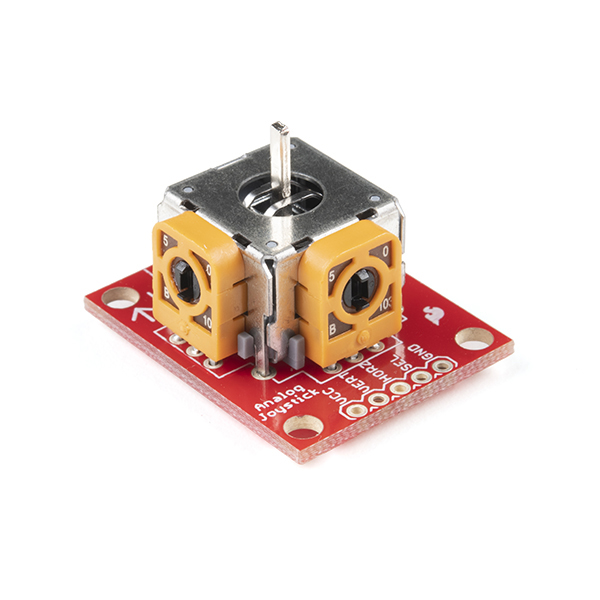
\includegraphics{diagrams/oem/16273-Thumb_Joystick_-_Deluxe-03.jpg}
    \caption{Joystick on BOB-09110 Breakout Board, from sparkfun.com}
    \label{fig:js2}
\end{figure}

The element of the unit remaining to be designed at this moment is the 3D printed housing. This is intended to attach to the clarinet in place of the button expansion, allowing for three different elements of control on the thumb rest. However, utilizing the button expansion thumb rest with the joystick has proved less ergonomic than desired, and will be fine tuned.

The Volume Detection unit contains uxcell Microphone Sound Sensor Voice Detection Module. Like the Button expansion, this unit is housed in a 3D printed case and connects to the Main unit with a USB-C cable. The PCB diagram shown in figure \ref{fig:micExPCB} is perhaps the least complex of all of the boards created so far. It essentially acts as an interface for the breakout module and the USB-C connector. Like the joystick and main PCBs, there is a place to include the power indication LED. The module will sit on the majority of empty space on the board, and should be pointed towards the desired pickup area. If loose, a little glue can be used to help hold the module down to the PCB. 

\begin{figure}
    \centering
    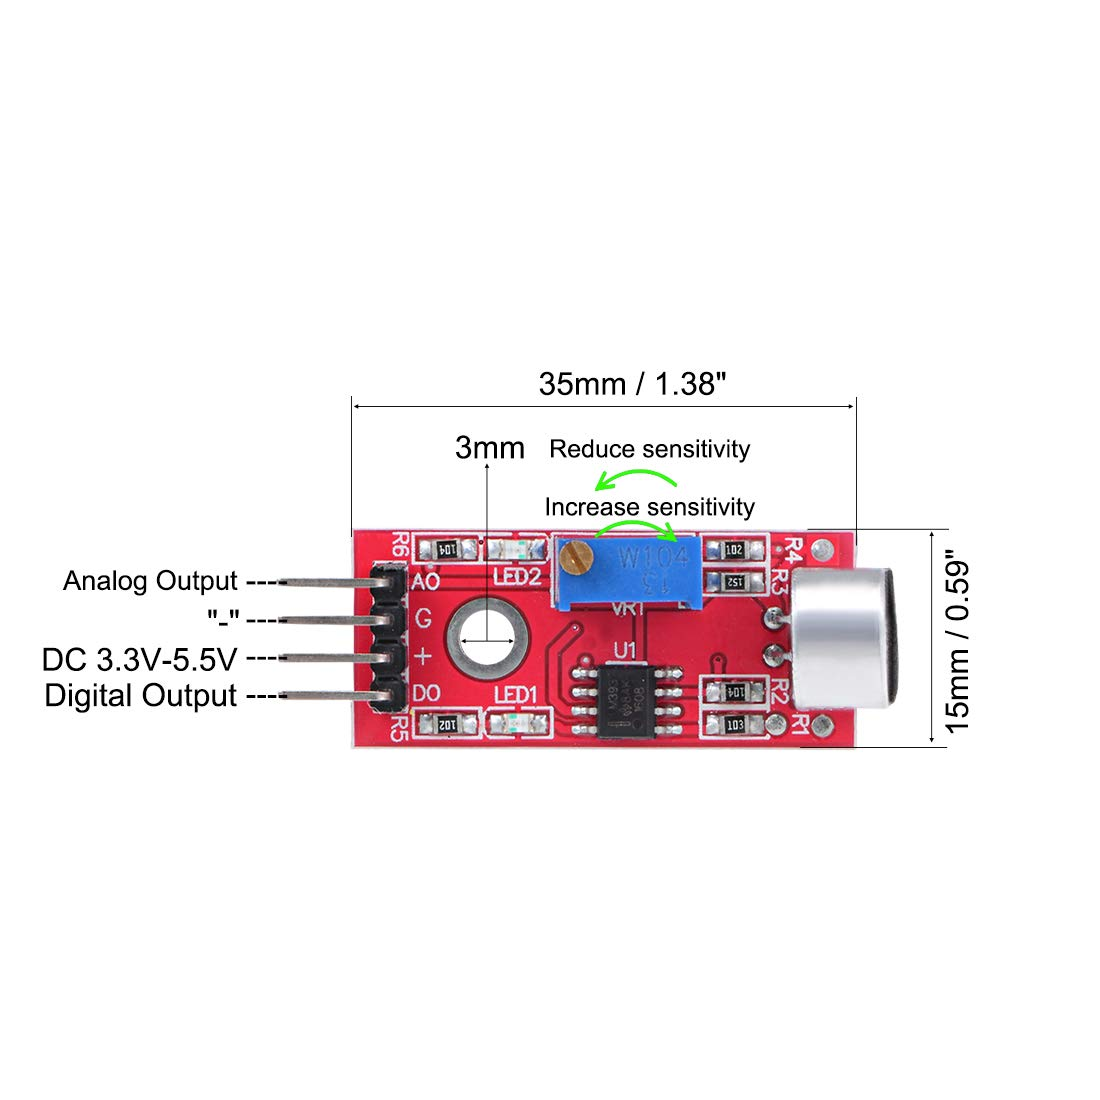
\includegraphics[scale=0.3]{diagrams/mic.jpg}
    \caption{uxcell Microphone Sound Sensor Voice Detection Module. Photo from amazon.com listing}
    \label{fig:micExpansion}
\end{figure}

\begin{figure}
    \centering
    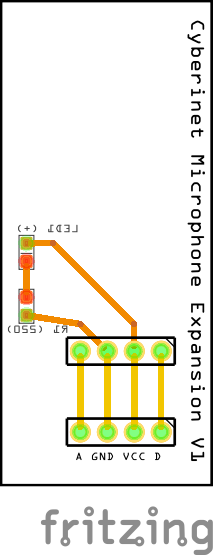
\includegraphics[angle=90]{diagrams/PCBs/micBasic_pcb.png}
    \caption{Microphone Expansion base PCB}
    \label{fig:micExPCB}
\end{figure}

This unit is designed to respond to the volume of the local area, and is designed to be placed in a variety of different areas. By placing the sensor at different distances from the performer or speakers, the sensor can more or less sensitively respond to the volume. The sensitivity can be adjusted with an on-board potentiometer and screwdriver. The user is only limited by the length of USB-C cable they can utilize. The Cyberinet detects when the volume at the sensor exceeds the given threshold from the on-board potentiometer, and transmits the data as a Boolean value to the computer in a similar manner to the Button Expansion. Future revisions will explore the uxcell Microphone Sound Sensor Voice Detection Module's analog outputs, but for now version 1 will only be utilizing the digital output due to its simpler and more reliable use cases. Ground and power connect to the middle two pins, and the data is returned on the pin marked D in figure \ref{fig:micExPCB}. This data is transmitted using the label exp1. 

Like the joystick, the 3D case is the final element keeping this unit from being further developed at the time of writing. The case is intended to entirely cover the microphone with the exception of holes for sound pickup, threshold adjustment, and viewing the LED. The unit is also intended to have a clip that can be used to attack it to various objects such as a music stand or the bell of the Cyberinet.

\section{Physical Design}
In order to minimize the total number of parts required to assemble the Cyberinet, the electronics are housed in a newly designed plastic unit. This Main Unit is intended to replace the barrel and mouthpiece of the original instrument when in use. In addition to the main unit, all expansions have a 3D printed body in order to control the expansion's ergonomics, protect the electronics, and aesthetically match the main unit.

\begin{center}
    \begin{figure}
        \centering
        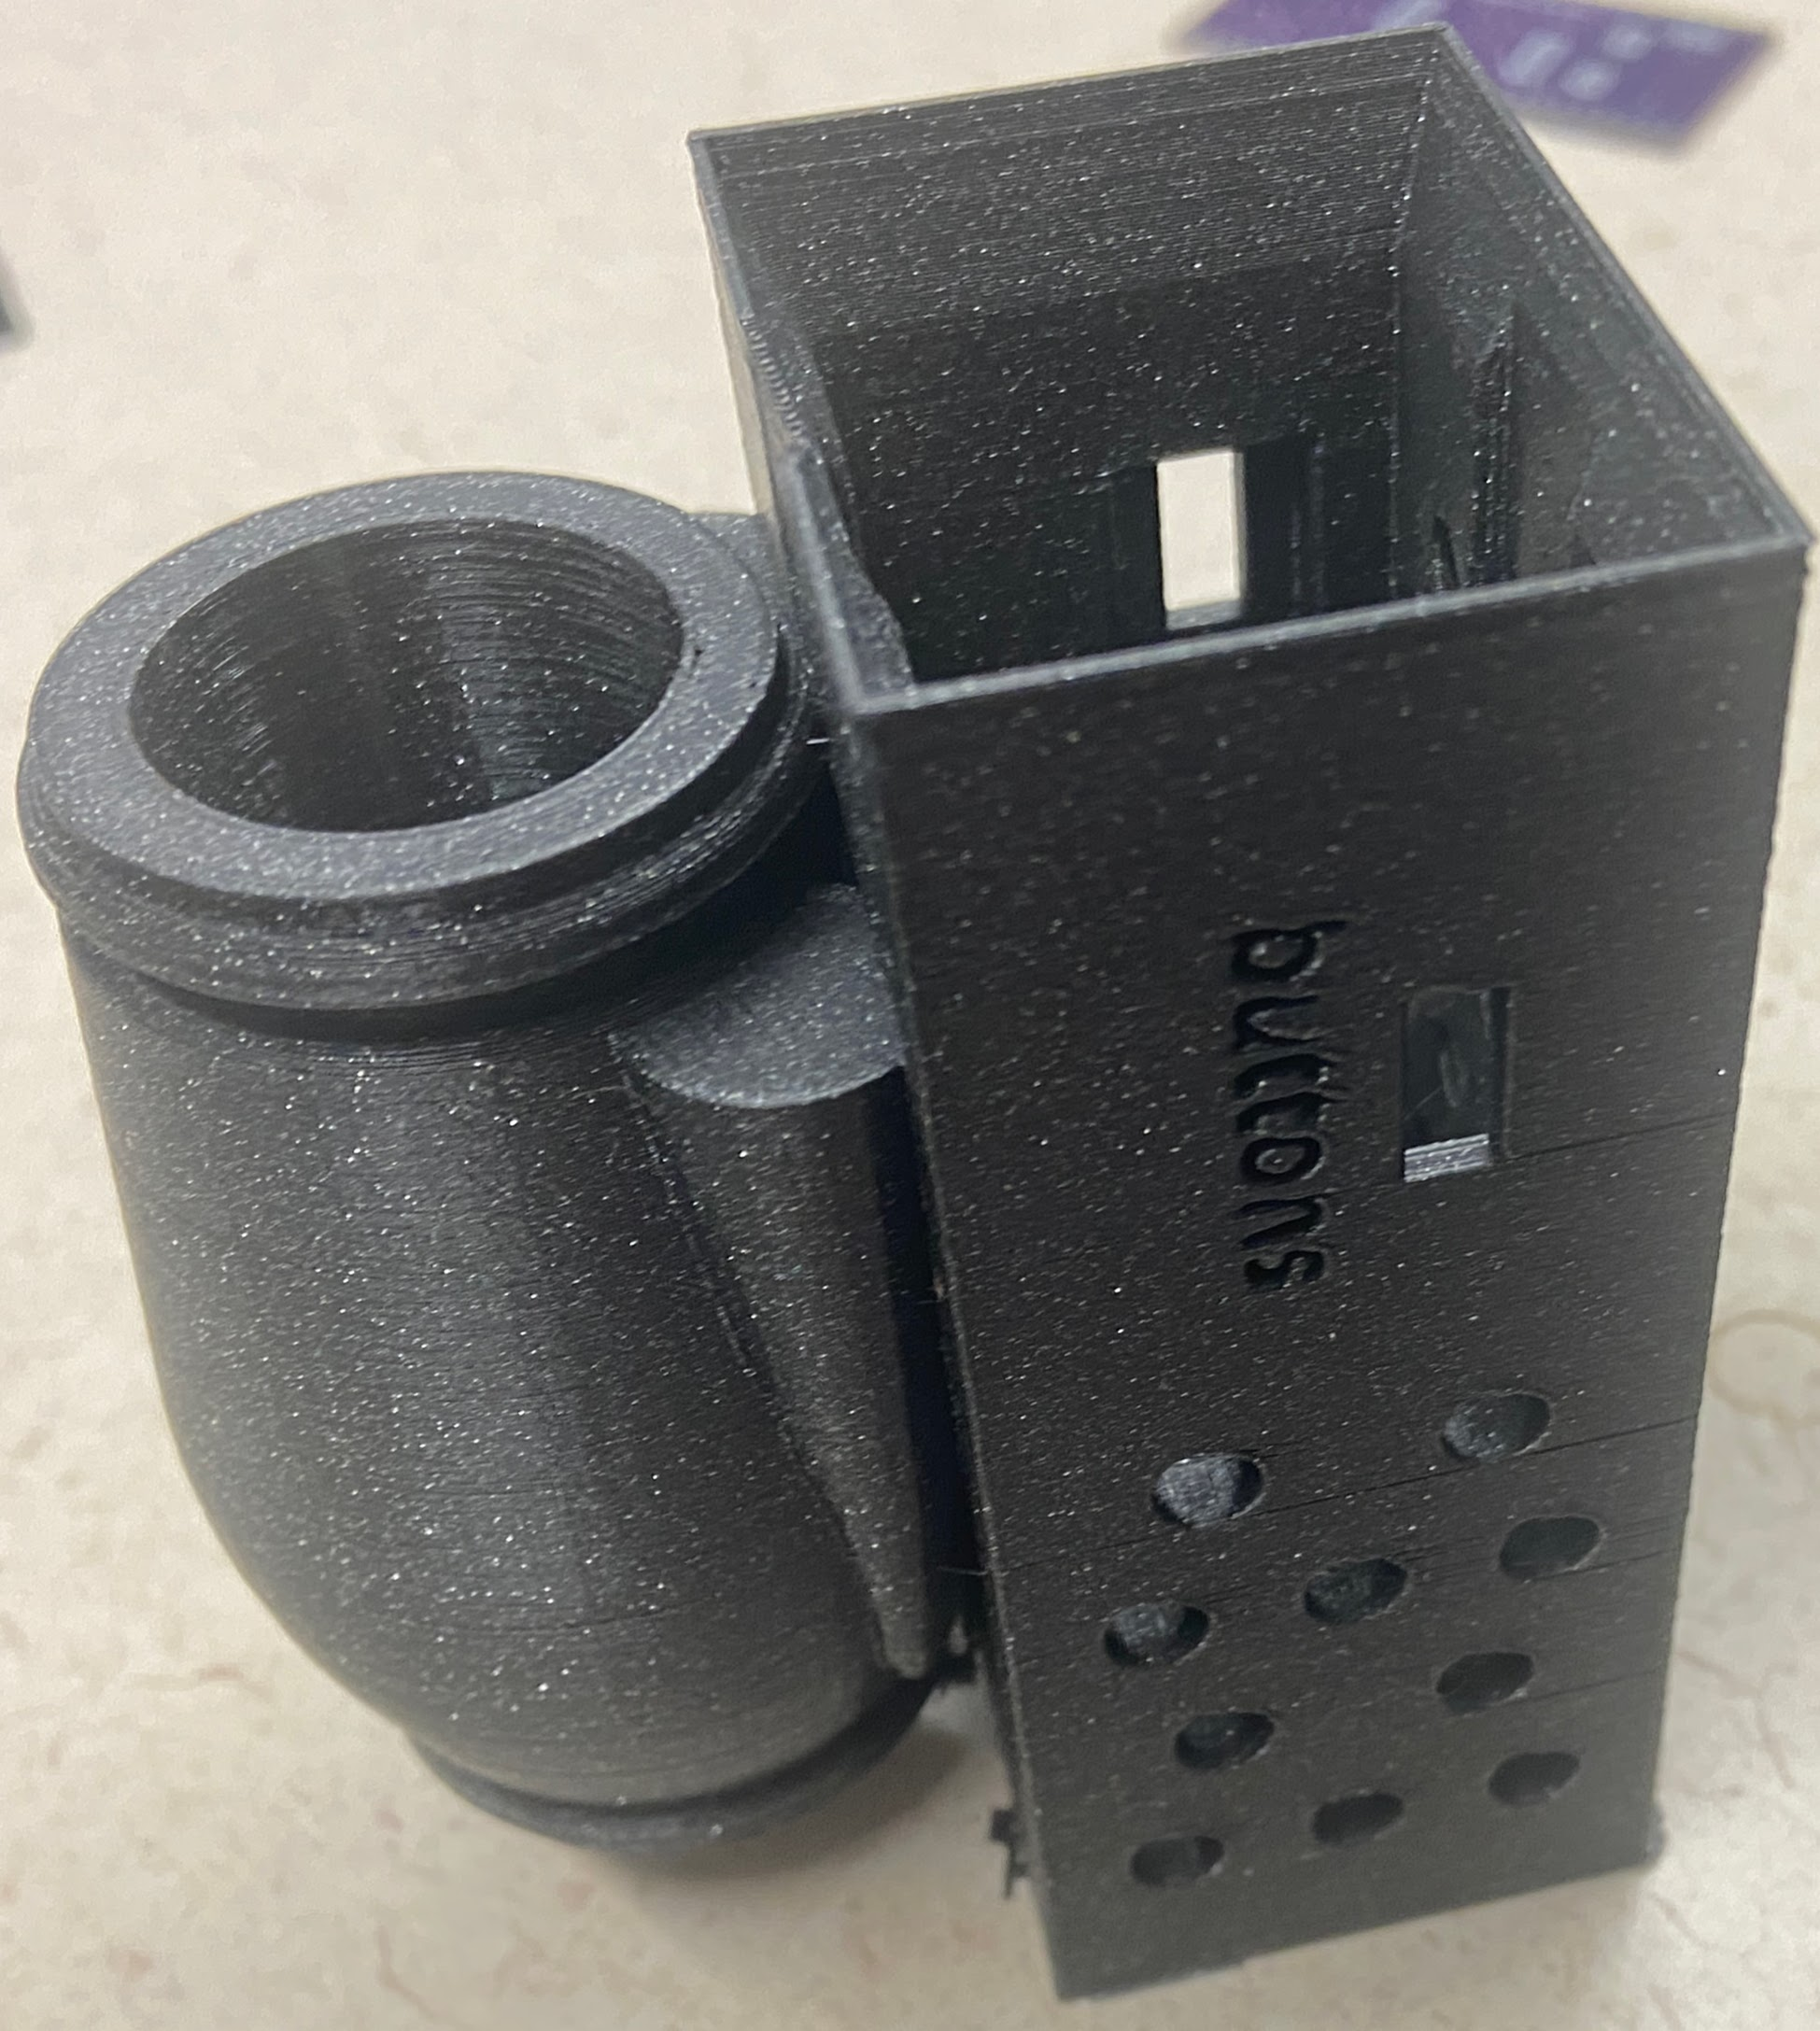
\includegraphics[scale=0.1]{diagrams/builtUnits/emptyCase.JPG}
        \caption{Empty 3D Printed Cyberinet Housing}
        \label{fig:cybernetCase}
    \end{figure}
\end{center}

All materials are printed using either PLA or PetG material during prototyping. These materials were chosen for their relative low cost, ease of production, and density. For the final version, PLA was utilized because the sound quality of the material most closely resembled that of the original clarinet. All parts were printed on an Original Prusa i3 MK3S+, with a 30-40\% infill setting. The final version was printed to be black or dark grey, however future revisions could see an option for custom colors when printing.


\subsection{Cyberinet Assembly}

The main unit of the Cyberinet is designed to replace the uppermost portions of a B-flat clarinet: The barrel and mouthpiece. As shown in figure \ref{fig:cybernetCase}, the electronic components are housed in the box on the side of the instrument. Placing the electronics here allows for the unit to be easily adjusted for tuning or be easily removed as needed. The box was made as small as possible, but it still contains all of the electronic components, excluding those in any external add-on components. 

The electronics were housed in the upper portion of the clarinet for two main reasons. The more minimal of the reasons is that the differential airflow pressure is much greater in the clarinet before the air can escape through the key holes. By locating the sensor here a wider range of values are possible than if it was located lower on the clarinet's tube. However, this could be remedied with additional tubing if the location of a unit needed to be otherwise located.

To assemble a Cyberinet main unit, first the case must be 3D printed. Because of the process of 3D printing and the necessary thickness of the material needed to preserve sound quality, the printing process takes approximately 12 hours to complete. Because of this, it is recommended to begin printing the case first, then work on the remainder while the case is being completed by the printer.

All components are connected utilizing a custom printed circuit board. This is done to help connect all of the various pins for data collection and power distribution in as small of a space as possible. 

\begin{center}
    \begin{figure}
        \centering
        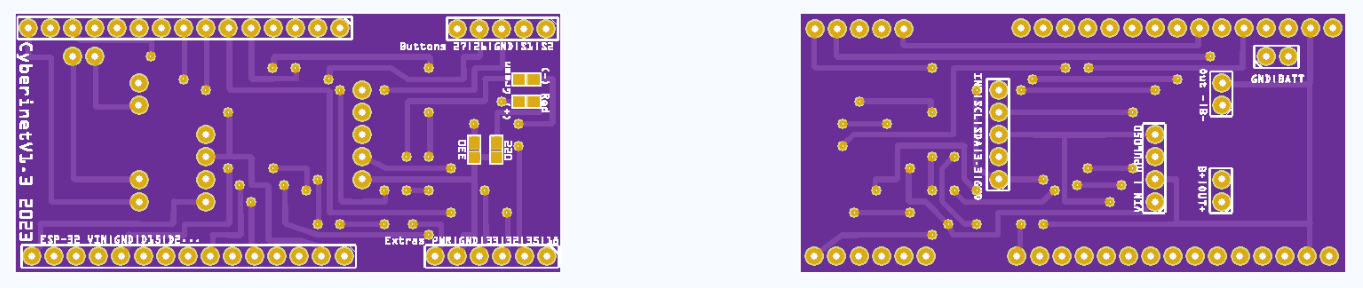
\includegraphics[scale=0.6]{diagrams/PCBs/cyberinetPCB.png}
        \caption{Cyberinet Version 1.3  Main Unit PCB Diagram}
        \label{fig:mainUnitPCB}
    \end{figure}
\end{center}

Assembling the Cyberinet must be done by working with the smallest components and working up to the larger ones. This is because several components are placed over other ones and it becomes exponentially harder to assemble a Cyberinet should one have to begin working around the placement of a sensor or remove a chip to adjust or repeat a step\footnote{It is recommended to pause and check the connections after soldering each component for this reason as well.}.

First, the Surface-Mounted components are soldered onto the main board. These include the 2 on-board LEDs and their accompanying resistors. Following this, ribbon cables and the USB-C and JST connectors are then soldered into place on the PCB. The ribbon cables are located on the five and six pin sections in the middle of figure \ref{fig:mainUnitPCB}. The connections for the button expansion and the other expansions are labelled due to the differing number of pins and their arrangement for the units. The JST connector is attached to the traces labeled GND and Batt. These connections attach the the USB-c connectors and the 1200 mAh battery respectively.

The third step is to solder the power distribution (TP-4056), gyroscope (MPU-6050) and airflow pressure (SDP-31) chips into place. The white silkscreen rectangles show which side of the PCB each component belongs on, and the text indicates which orientation is needed for each component to help ensure a correct alignment. This is also present for the connections that have already been mentioned.

The airflow pressure sensor (SPD-31) is lifted away from the PCB with the use of a pin header. This is done to avoid any accidental shorts between the contacts on the two boards. While not required, this can be done to the gyroscope (MPU-6050) as well for the same reason. The final soldering step is to connect the ESP-32. Because of its size, this chip is kept opposite from the sensors and is also lifted using pin headers to avoid any accidental short circuits.

\begin{center}
    \begin{figure}
        \centering
        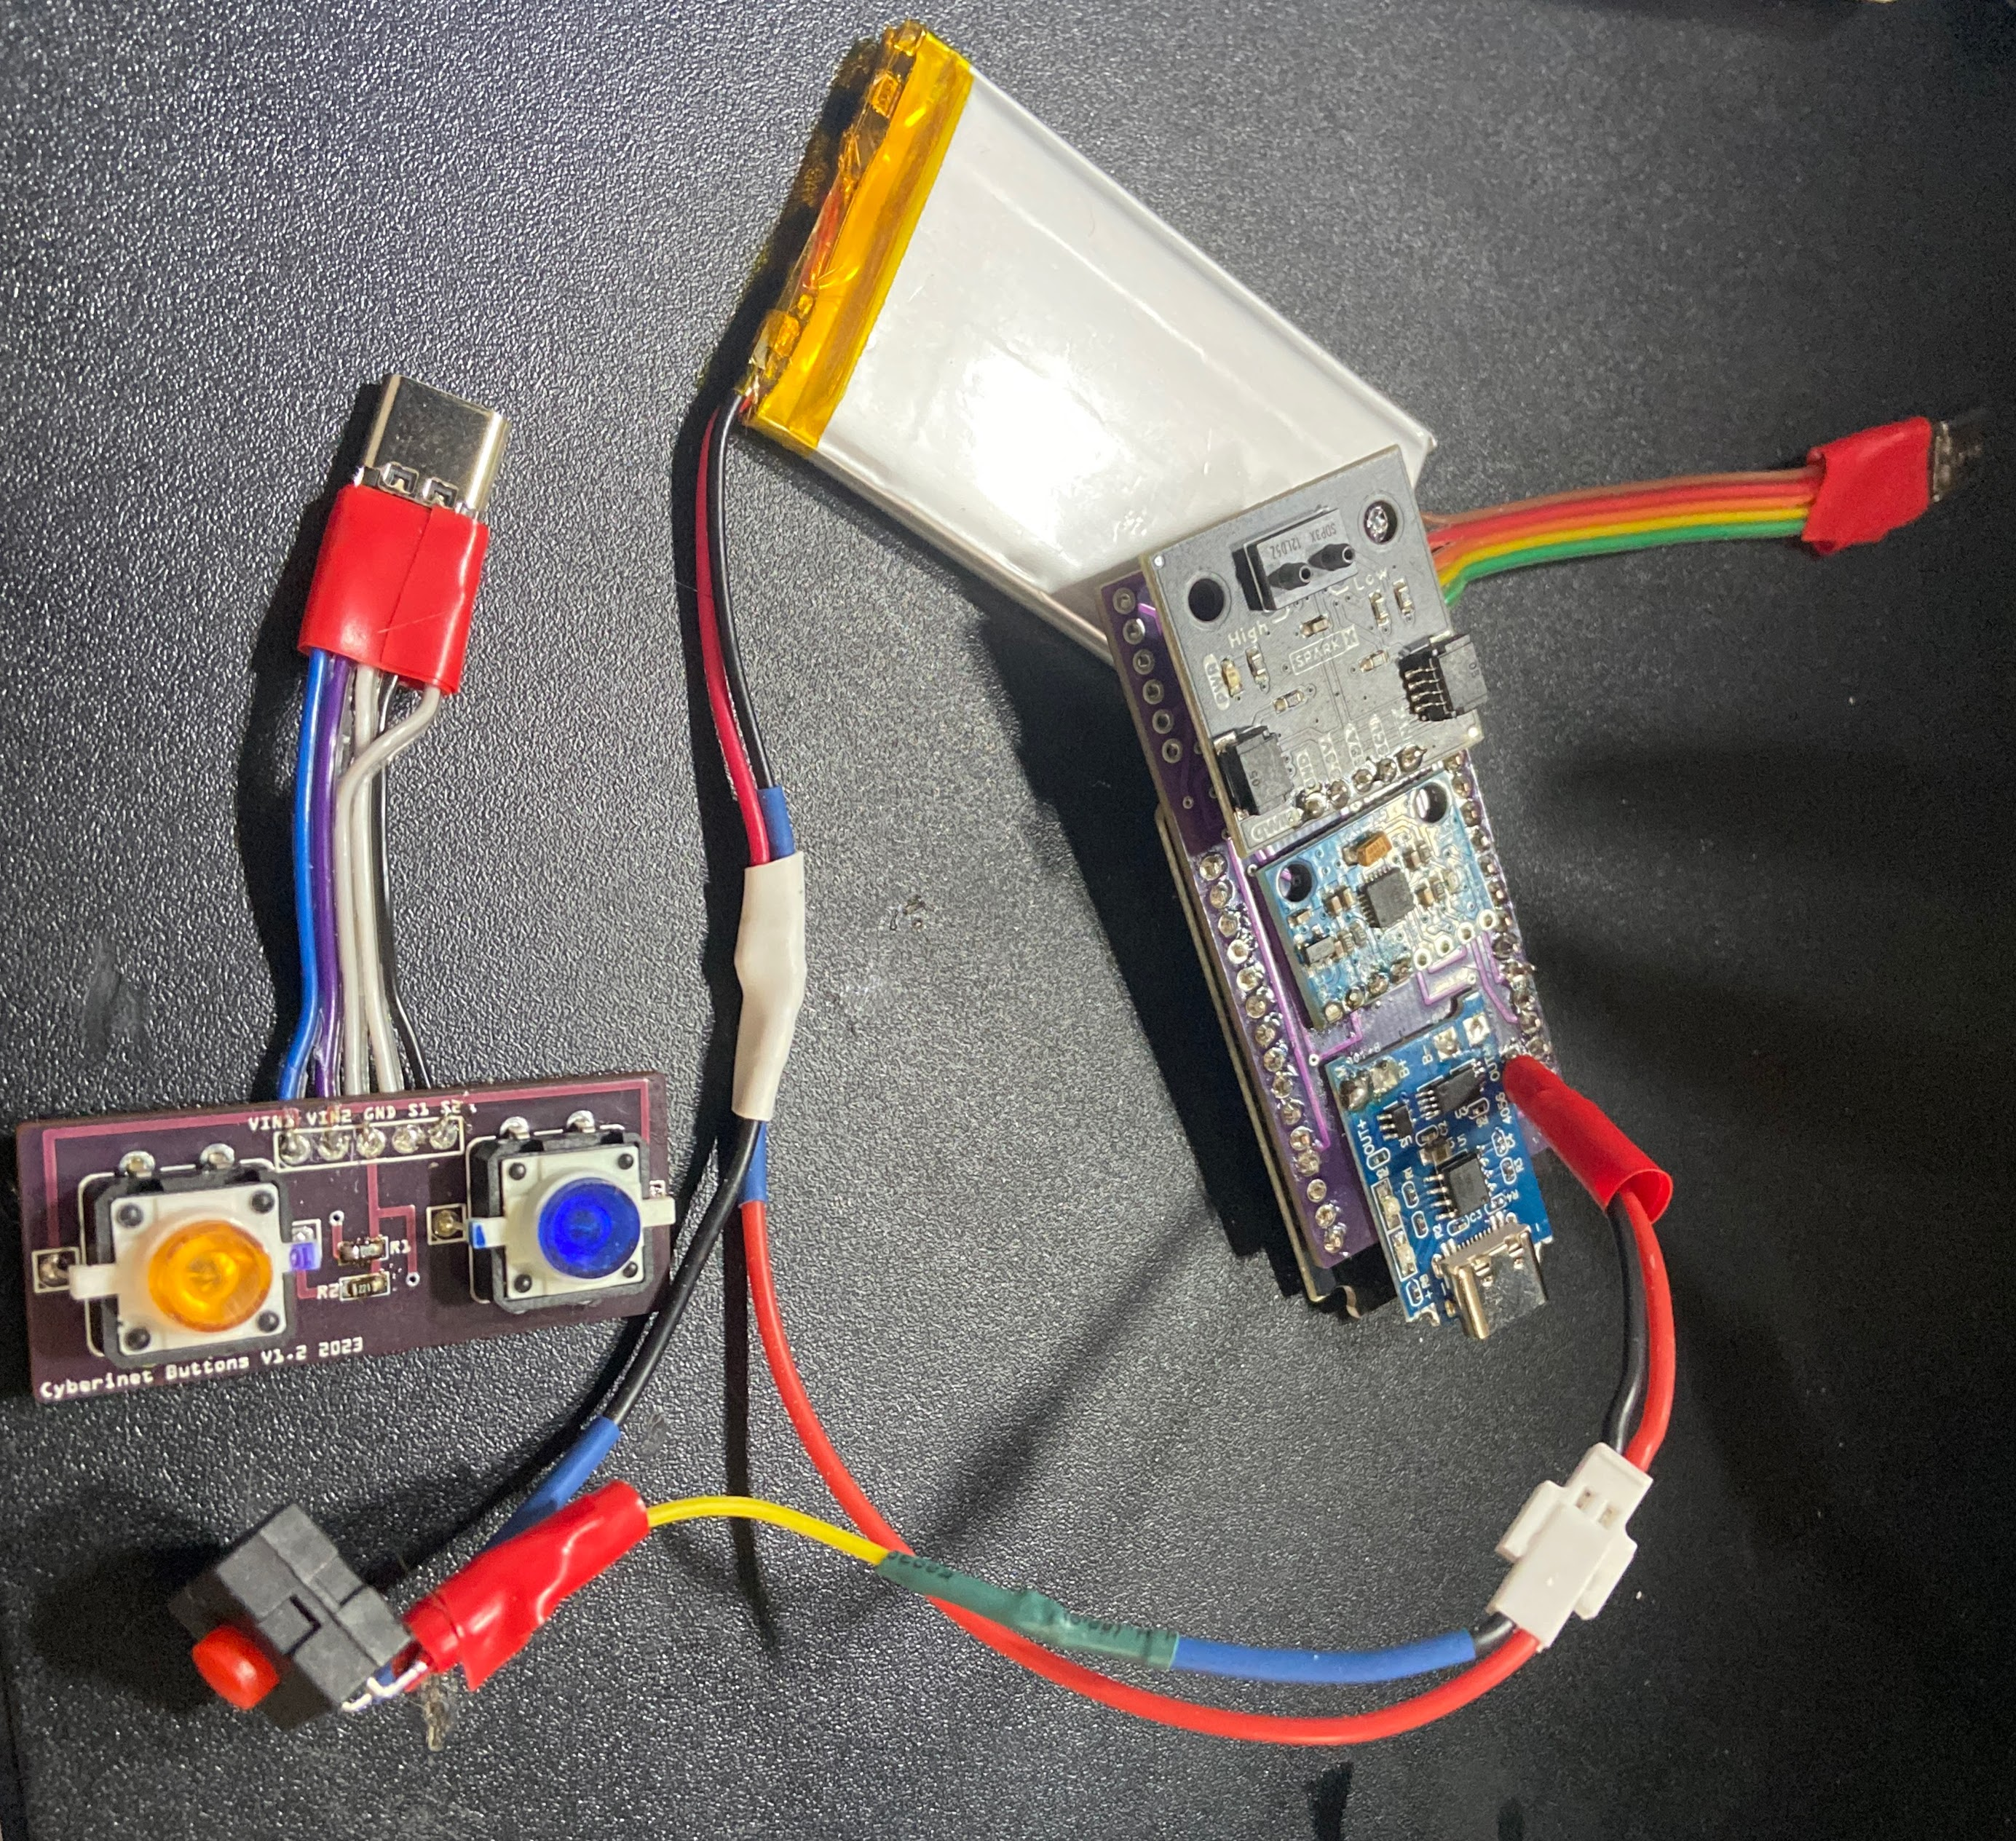
\includegraphics[scale=0.1, angle=90]{diagrams/builtUnits/noCase.JPG}
        \caption{Completed Cyberinet and Button Expansion without 3D printed housings.}
        \label{fig:CyberinetNoCase}
    \end{figure}
\end{center}

When complete, the whole unit is slid into the 3D-printed case. Ports and tubes are aligned to the appropriate places and glued down to avoid unwanted movement. Not taking into account the space needed for the battery, tubing, and wired, the final Main PCB is approximately 5mm deep, creating a compact unit that can be easily placed in a variety of locations. When the battery is included, the depth is approximately 9mm.

\begin{center}
    \begin{figure}
        \centering
        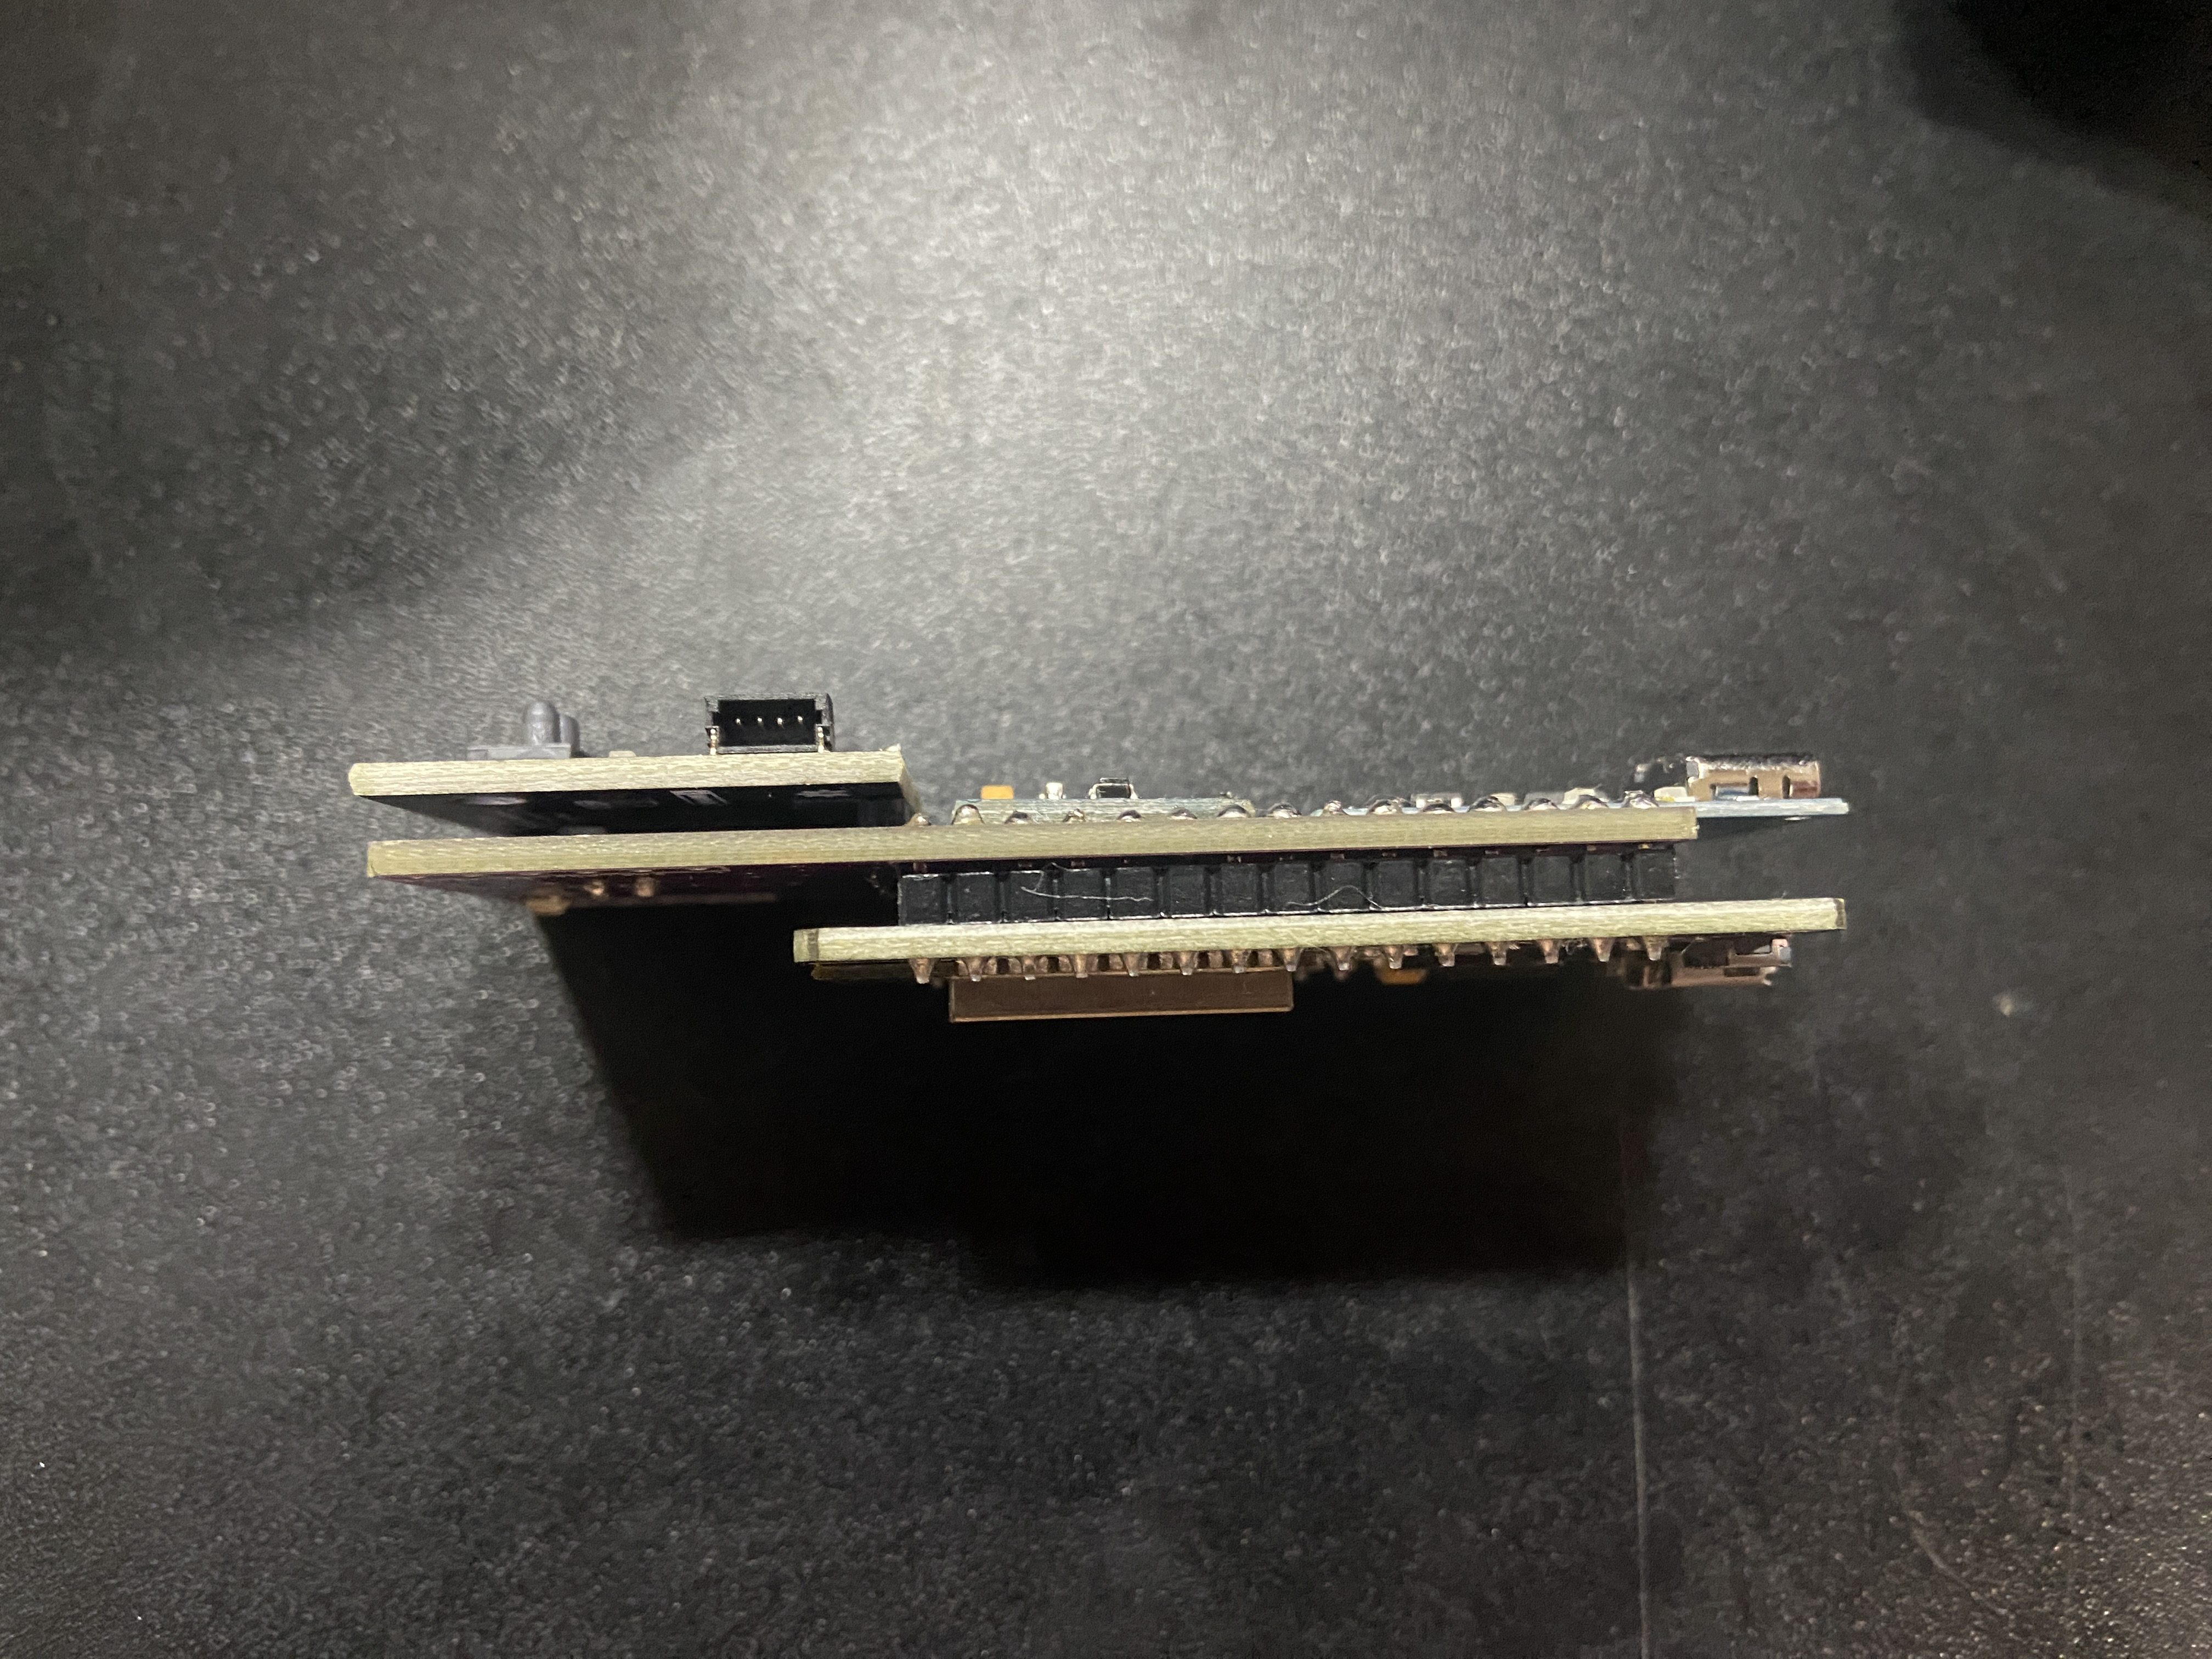
\includegraphics[scale=0.05]{diagrams/PCBs/cyberinetThin.JPG}
        \caption{Cyberinet Sensors Side View (No Casing or cables)}
        \label{fig:Cyberinetside}
    \end{figure}
\end{center}

Once the internal electronics have been inserted, secured, and sealed into the 3D printed case, it is ready to be fully tested. Because the Cyberinet unit cannot be easily opened, and will require glue to reseal, it is recommended that all base functionality be tested prior to closing the housing. While close, no two clarinets are completely identical, so the internal sides of the 3D printed case may need to be sanded to properly fit onto the clarinet with cork grease applied. Overall, placing the Main Unit's bulkiest components as close to the performer's mouth as possible results in the least amount of extra effort required to perform with the instrument. It is impossible to completely remove the added weight of the system additional, but this placement minimizes its impact on the performer.


\chapter{Programming \& Using the Cyberinet}
This chapter discusses the code located within the Cyberinet itself, as well as the accompanying library of Max tools and how they can be utilized in a performance. The Arduino code and the Max objects work together in order to achieve the five main steps in the functionality loop of the Cyberinet. 

\begin{itemize}
    \item Step 1: Collect Data
    \item Step 2: Transmit Data
    \item Step 3: Receive Date
    \item Step 4: Route Data
    \item Step 5: Utilize Routed Data
\end{itemize}

The functionality is not a full loop from steps one to five. By this I mean that once the data has been transmitted, the hardware will repeat the sensing and transmitting process while the computer will route and apply the data in a separately timed loop. The communication is not two-way between the computer and hardware unit, but the computer-side loop is unable to begin without the completion of the hardware loop. Combined with data smoothing within Max, the end result is a constant stream of data between the two with minimal latency.

\section{Arduino Code}
Another positive feature of the ESP-32 is that it is able to be programmed utilizing a variety of languages and environments. For the Cyberinet, the micro-controller was programmed using the Arduino coding language and Arduino IDE version 1.8\footnote{Arduino IDE Versions 2.0 and 2.1 were both released during the Cyberinet's development, but were not utilized to avoid any potential compatibility issues during development. Future software versions will be created in more up-to-date IDEs.} The full .ino file can be found in this document's appendices.

\subsection{Collecting Data}
In order to collect the data from the sensors, each sensor has been given a function within the Arduino code. These functions serve the main focus of collecting and transmitting data. However because of the differing OEM sensors, each one utilizes a slightly different method of data collection and has a different range of values that can be expected. These functions are called in every loop of the program. Figure \ref{fig:getButtonsGetAir} shows the two most straightforward of these functions in their entirety.

\begin{center}
    \begin{figure}
        \centering
        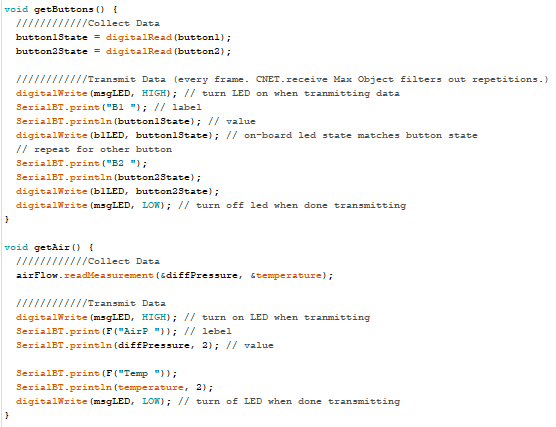
\includegraphics[scale=1.5]{diagrams/maxPatches/getbuttonsgetair.png}
        \caption{Cyberinet getButtons() \& getAir() functions.}
        \label{fig:getButtonsGetAir}
    \end{figure}
\end{center}

The function getButtons() is the simplest of these functions. This function looks at pins 12 and 14 on the ESP-32, which are connected to the Button Expansion's USB-C connector. By utilizing the ESP-32's built-in pull-up resistors, the Button Expansion returns a 1 when the button is not being pressed and a 0 when the button has been detected as being clicked.

getAir() works in a similar function to getButtons(), but with a slightly different code because of the SDP-31's I2C connection and coding library. Because of this, the ESP-32 contacts the SDP-31 on its I2c address and requests the specific data at 2 registers. These data are labelled as 'diffPressure' and 'temperature' respectively. 

The function 'get5060()' is shown in figure \ref{fig:get6050}, and contains a few more complicated steps than the previous functions. This function begins by communicating with the MPU-6050; essentially waking it up after having communicated with the SDP-31 on the same pins. Next, the data points for the gyroscope and accelerometer are requested like 'diffPressure' and 'temperature'. It is at this point that the function begins to differ from the others.

\begin{center}
    \begin{figure}
        \centering
        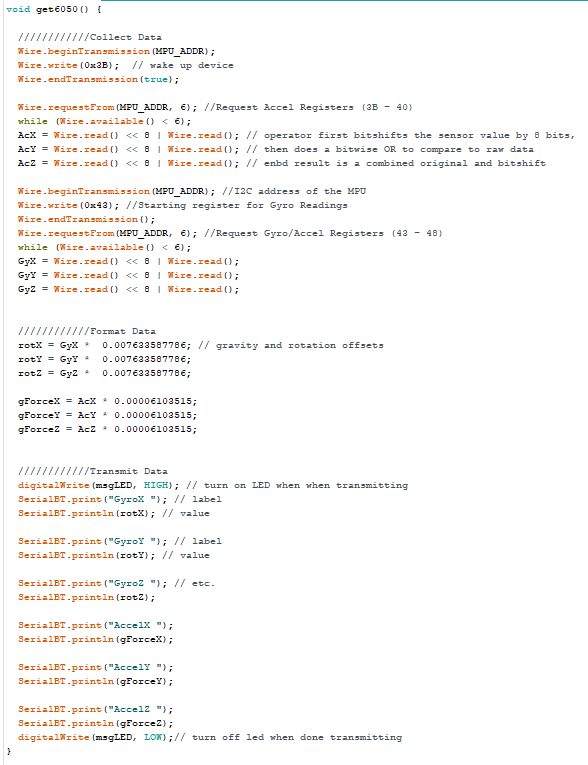
\includegraphics[scale=1.5]{diagrams/maxPatches/get6050.png}
        \caption{Cyberinet get6050() function.}
        \label{fig:get6050}
    \end{figure}
\end{center}

All six of the requested data points are then shifted over by 8 bits and then added to a second reading of the remaining data. This is done in order to fully read all 16 bits of data from the MPU-6050 on devices unable to access and process all 16 bits of data at once. Prior to transmitting the data, the values from the MPU-6050 are then scaled. This is done to compensate for both the gravitational pull and rotation of the earth, allowing for more accurate results. This step is done here rather than in Max to eliminate the potential of a user not scaling the data within Max.


\subsection{Transmitting Data}
The final portion of the data collection functions is the transmission of the data. This is done using the bluetoothSerial library, which allows for the ESP-32 to utilize serial communications over a Bluetooth connection. The .ino code's setup function is responsible for setting up these connections. The port is titled "CyberinetV13", indicating the version number with no spaces or punctuation, and utilizes a baud rate of 115200\footnote{In short, the baud rate is the number of changes to the state changes within a digital signal.Larger values allow for more data transmission, if the device is capable of handling the increased data rate}. This library contains the main Serial functionality present in Arduino, and simply is called with the instance name SerialBT to indicate the transmission is a wireless one.

Once all of the data is collected within a function, it is transmitted using the SerialBT.print() and SerialBT.println() commands. Utilizing the Max formatting, a label is created for each data point being transferred, then the individual value is transmitted, separated from the label with a space and ending with a carriage return. Each of the labels are listed in figure \ref{fig:sensorLAbels}. Each sensor receives its own unique label. However, this is technically only true for the sensors present in the main unit. Because they share the same port and have a varying number of pins for returning data, the expansions all utilize the label 'exp' followed by the number. The expansion port contains six pins: power, ground, and four data return pins. Be keeping the data return format consistent between all expansions, it eliminates the need to identify the sensor in the moment. The main downside is that the user will have to remember what the sensor was in the programming environment, but this can be easily rectified with comments, notes, and looking at the physical units being utilized.

\begin{figure}
    \centering
    \begin{itemize}
    \item gyroX
    \item gyroY
    \item gyroZ
    \item accelX
    \item accelY
    \item accelX
    \item airP
    \item temp
    \item b1
    \item b2
    \item exp1
    \item exp2
    \item exp3
    \item exp4
\end{itemize}
    \caption{Sensor labels used when transmitting data withe the Cyberinet}
    \label{fig:sensorLAbels}
\end{figure}

The data is sent in serial data packets, and the spaces and carriage returns are utilized by Max to help isolate the individual data and label values. The raw data stream as it appears in the Max console is shown below. To indicate that a data transmission has occurred, the red message LED is illuminated immediately before and toggled off immediately following the completion of the transmission. The end result is a rapid blinking of the red light when the Cyberinet is functioning properly. When combined with the green power indicator LED, the result can be perceived as a light changing between green and yellow through the holes in the 3D printed case. The measured latency of the data transmission is measured at approximately % finish testing 
That value was repeatedly testing with the CNET.latency patch. In order to arrive at the averages shown in figure % need to make figure with values after testing.

CNET.latency can be utilized by anyone who needs to test the latency of their hardware unit. When loading the patch, and connecting the Cyberinet, a microphone and the button expansion are also needed. The user will place the microphone close to the buttons and press one of them which makes an audible click. This audible click is recorded, and then used to gate a small burst of white noise, which then is output from the speakers and picked up by the original microphone. Max then compares the number of milliseconds between the first button click and the burst of white noise from the speakers. This comparison calculates the full latency from an action on the Cyberinet to its result being herd by the user. Because the majority of latency occurs in the wireless data transmission, this is a good indicator of the transmission speed.  

\section{Max Programming}

To utilize the data being collected by the Cyberinet’s hardware, a small collection of Max objects to help with the collection and usage of said data have been developed. These allow the user to easily implement common effects and the mapping of gestures to effects without needing to worry about compatibility between the objects. It is important to mention that Max is a paid software. The software and hardware components are all open source, however in order to create your own patches, the end-user will need to download the software. If saving patches is desired, then they must purchase a software license. 

Prior to utilizing the CNET objects, however the data being transmitted from the Cyberinet must be received and routed.



\subsection{Receiving \& Routing Data}

When implemented, the CNET objects are utilized to help receive and route the data within a Max patch. Once the sensor data has been transmitted from the Cyberinet utilizing the SerialBT.println() command in the Arduino code, it moves into the connected computer. This connection utilizes Bluetooth, and can be easily managed in the Max software\footnote{Max version 8.5.x or newer is needed when working with the Cyberinet}. A single object is utilized in order to help receive and parse the data stream from the Cyberinet. CNET.receive allows the user to easily configure which Bluetooth port to receive data from, then sends that data to various outlets for use in the Max environment. The internal workings of CNET.receive are shown in figure \ref{fig:cnet.receive}. There are three main subsections to CNET.receive that allow it to function.


\begin{center}
    \begin{figure}
        \centering
        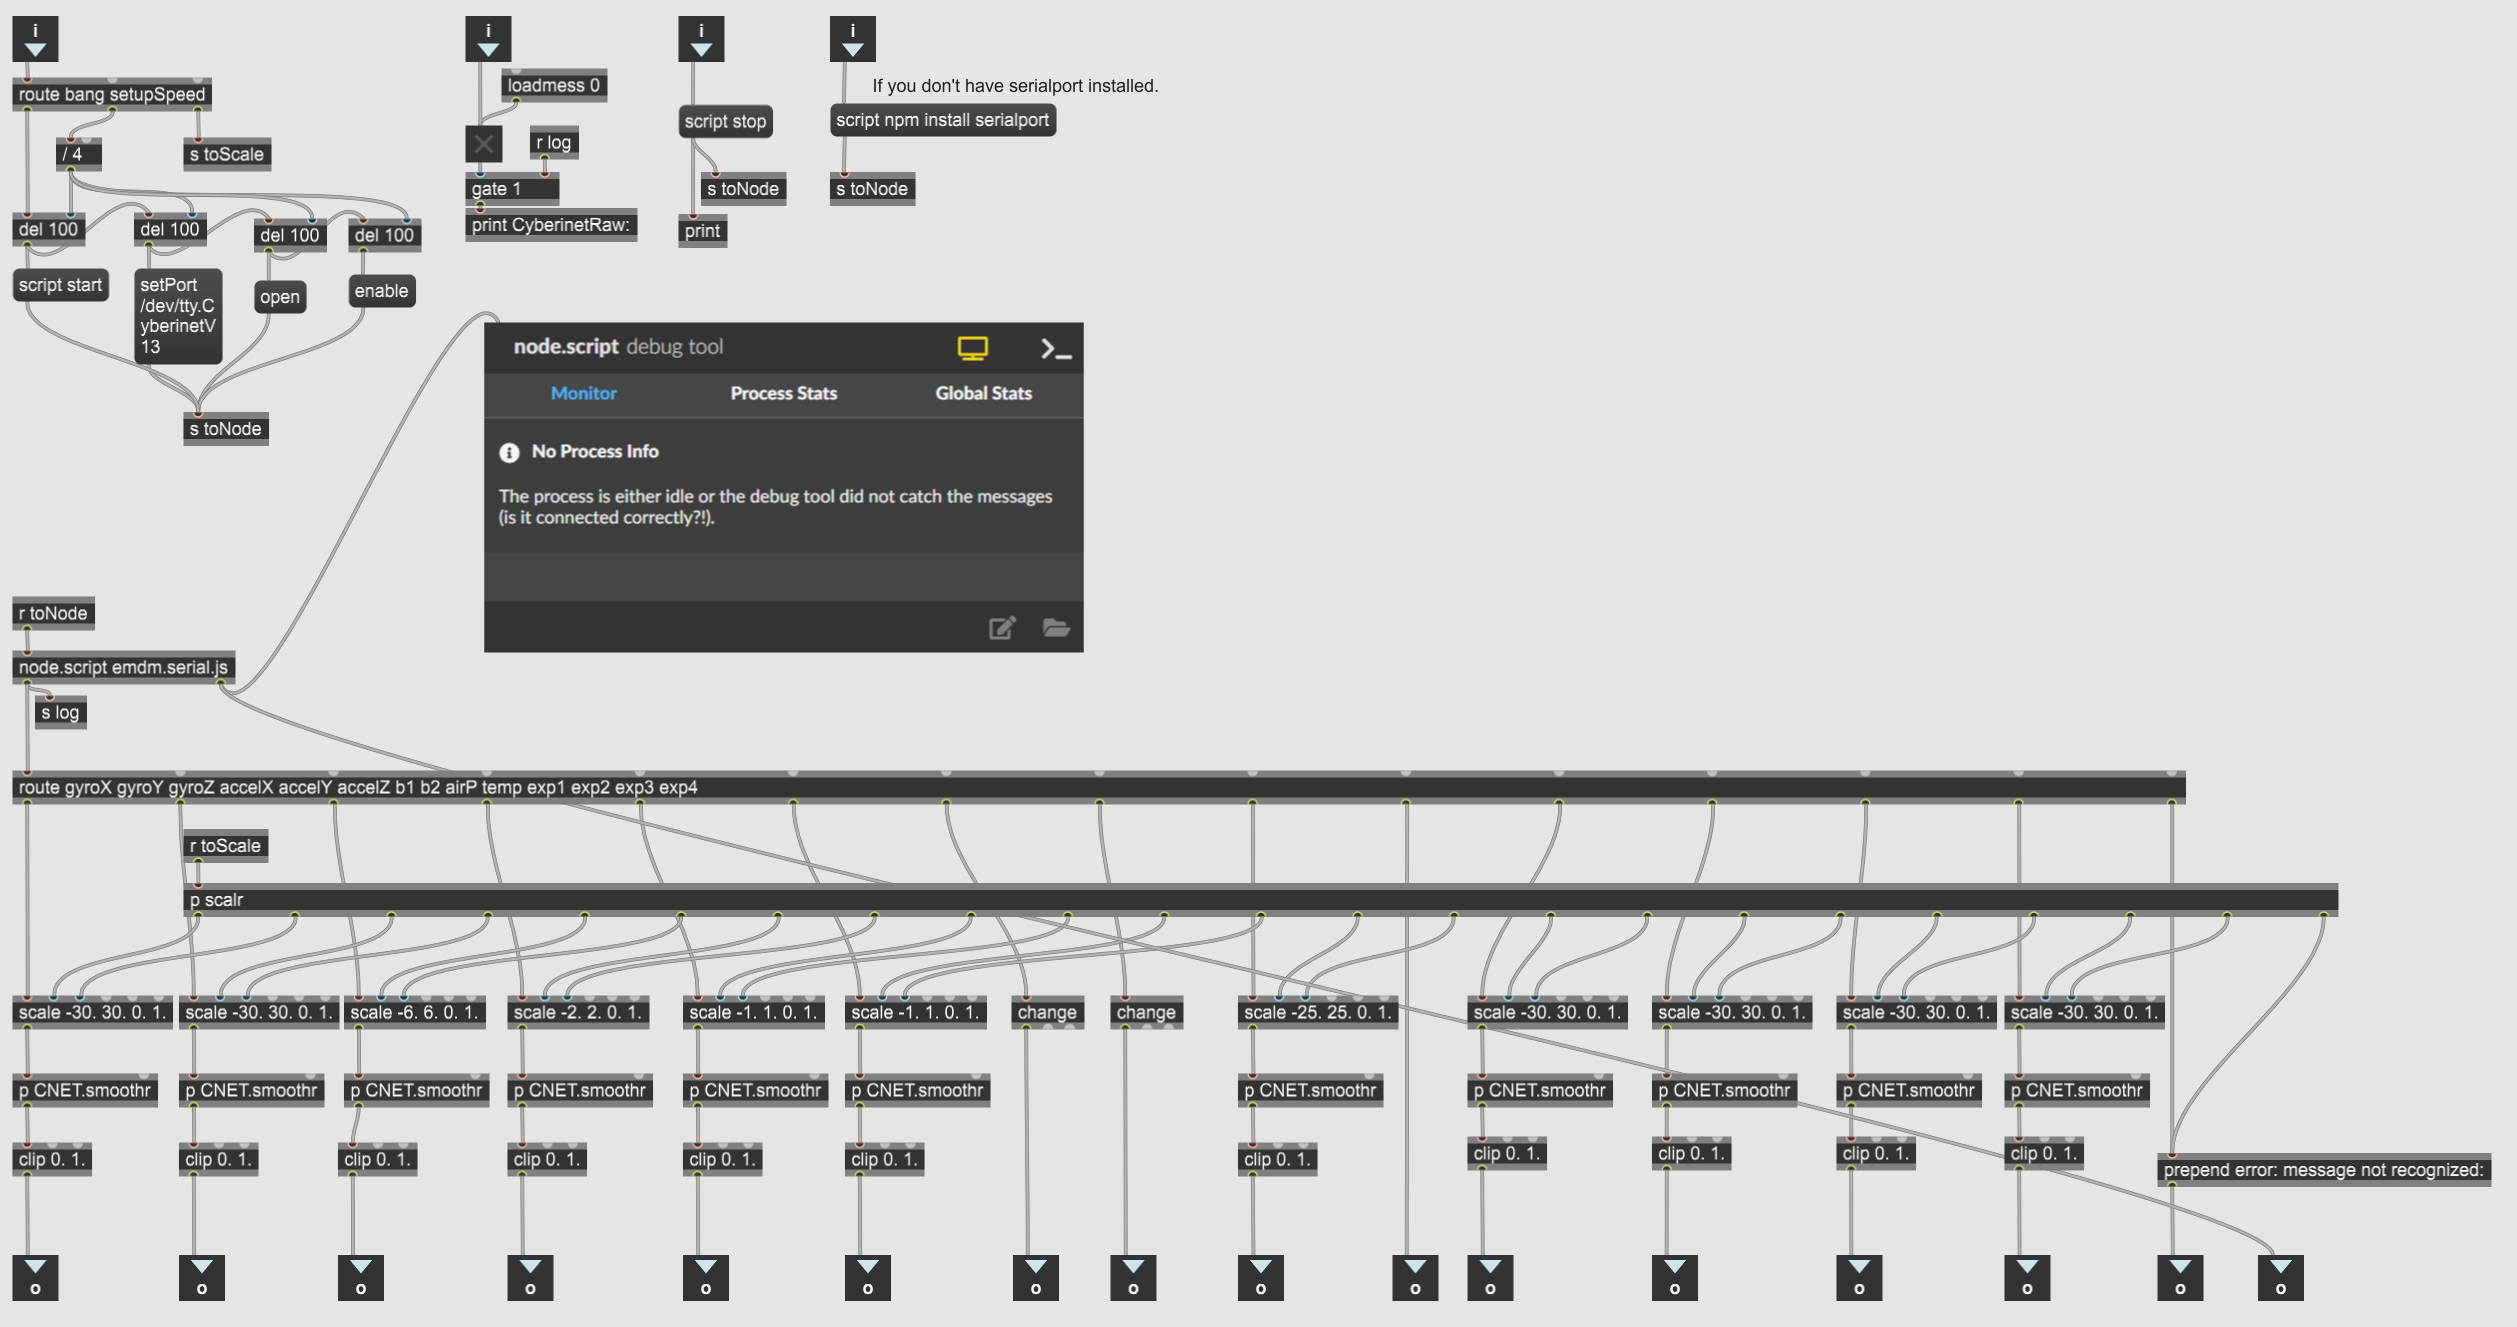
\includegraphics[scale=0.48, angle=270]{diagrams/maxPatches/CNET.receive.png}
        \caption{Inner workings of CNET.receive}
        \label{fig:cnet.receive}
    \end{figure}
\end{center}

The top section of figure \ref{fig:cnet.receive} shows the setup for beginning communications with the Cyberinet. A bang into the first inlet will begin running a node JavaScript file. This file helps max to communicate with the given port, respond to the data, and give feedback to the status of these communications in the Max console. The Node js debug tool can be helpful when monitoring the status of CNET.receive as well. Inlet two will toggle the printing of the raw data within the Max console in real time. This is useful, but can quickly take up computer memory due to the large number of data points being transferred. Inlet three stops communications, and inlet four will install the various node dependencies when banged\footnote{This is only necessary if a computer does not already have these files installed. Once this has been done once, it is not needed unless moving to a new computer or node was removed.}. 

When setting up communications, the initializing bang is actually achieving multiple steps. These were condensed in order to simplify and streamline the process. A single bang will begin the node script, set the port, open the port, and begin communications. A short delay is given between each of these steps. This is needed to give the computer enough time to respond to the messages. It is recommended to not change this, but if needed the time can be adjusted with the control message "setupSpeed X" where X is the total delayed duration in milliseconds. that value is divided by four and equally applied to each internal delay object. All other control messages are used with CNET.rangeSet.

The middle section of the patch contains the node script\footnote{the full code of the node script is given in Appendix B} and a route object. The base for the node script came from a collection of objects created by LSU's Experimental Music \& Digital Media department. All this script does is receive the raw data on the indicated port and outputs it as a data stream. The route object then parses the data based on the accompanying label from the Arduino code. Each label from figure \ref{fig:sensorLAbels} is utilized within the route object. The routing removes the label, outputting only the accompanying data values to their designated outlets. The data is then formatted for its final use outside of CNET.receive.

The final section of CNET.receive contains a large number of objects, but the process is repeated for the majority of the sensors. The sub-patch called "scalr" simply parses the lists from CNET.rangeSet if that object is used and applies it to the appropriate scale objects below. These objects take the raw values from the Cyberinet hardware and proportionally adjust it to fit a range of 0-1. If a performer is generating a range of raw values that are too large or small for the desired effect, the internal scaling can be adjusted without altering the output range. The sub-patch "CNET.smoothr" is used for the final manipulation of the data, and is shown in figure \ref{fig:smoothr}. This object may potentially move into a more defined control object in the future, and is why it has a CNET name, despite not being a unique object in.

CNET.smoother takes incoming values and gradually slides between them instead of directly setting the values. This helps to make the effects sound continuous and minimize noise and popping. This defaults to being averaged over 20 data points. This value can be adjusted if needed, but experimentation is not recommended with this object. The second portion of this sub-patch compares the current smoothed data point with the previous one and calculates the difference between them. This value is then output back to the main patch, and clipped to the range of 0-1 to remove any outliers and avoid problems in the CNET effect objects. The result of this means that only when a sensor is actively picking up a gesture will it's data be utilized within Max. Using the gyroscope as an example, data will be output from CNET.receive while the instrument is actively rotating. When the performer is not performing a gesture, the values are almost zero.

The values cannot be completely zero due to the continual nature of the sensors and subtle changes to the performer's position and movement, the values are small enough to be unnoticeable in the majority of situations. Three sensors to not undergo this smoothing process due to their design. Both buttons only output values of 0 or 1. Smoothing those data points would remove the immediacy of a momentary switch. Instead, these values are output only when the button changes state. The only change to this data is that the binary data has been flipped from what was received from the Cyberinet. The hardware unit transmits a 0 when the button is pressed, but CNET.receive changes this to output a 1 when pressed and a 0 when released. This is the same for both buttons. The third sensor is the temperature sensor. While these values could be smoothed, the difference calculations prove to be problematic in this situation. Generally speaking, any temperature fluctuations large enough to be interpreted as a gesture would be extremely uncomfortable for everyone in the performance space, assuming they are possible to achieve in the first place. If made more sensitive to respond to smaller fluctuations, then the changes cannot be detected as a gesture. To avoid all of these problems, the temperature data is output completely raw in degrees Celsius. This is the only value to not be scaled, as having the accurate temperature would be more useful than a 0-1 value in most situations when that sensor would be used.


\begin{figure}
    \centering
    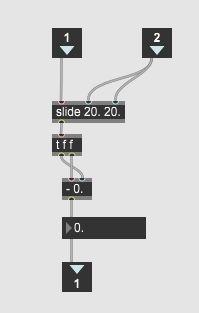
\includegraphics[scale=1.3]{diagrams/maxPatches/smoothr.png}
    \caption{Processing of smoothing and comparing the data stream within CNET.receive}
    \label{fig:smoothr}
\end{figure}

\subsection{CNET Objects}
The CNET collection of max matches works to interface the Cyberinet with Max in multiple different ways. Every object discussed as part of this collection has the prefix CNET, which is an abbreviation of the word Cyberinet. CNET can be broken into two main categories of patches based on how they interact with the Max Environment. Effect objects are largely commonplace audio effects that have been designed to work with the Cyberinet's data ranges. Control objects on the other hand are designed to manage the routing of data or provide feedback about the data being received by the various sensors.


Regardless of category, each CNET object has multiple inputs for those who want to utilize them to control the varied parameters for each object. These inputs are located immediately to the right of the main signal inlet, and are ordered to be a logical progression of controls from left to right. In the following section, each category of objects is listed with a short description. Each CNET object also has a detailed breakdown of its full control parameters, presets, and default values to show off the capabilities of the software both with and without a connected Cyberinet.

\subsubsection{Effect Objects}

Effect objects are commonplace audio effects, with the exception of CNET.dmx. All of these objects are intended to take in data from the Cyberinet and utilize it to alter the performance environment. This is done through the processing of an audio signal. CNET.dmx achieves this goal by outputting values to control DMX lighting, and does not operate at the signal rate. Because of the wide variety of potential sound options with the Cyberinet, a handful of commonplace effects were chosen in order to help the user be able to easily create interesting effects that anyone with general musical knowledge would be able to easily implement. The current list of CNET effect objects is:

\begin{itemize}
    \item reverb$\sim$: A Schroder style reverb based on examples from CCRMA and John Chowning. this has a stereo output, and is similar to effects like JCReverb.
    \item monoReverb$\sim$: The same reverb above, but with a mono output instead of a stereo one.
    \item compressor$\sim$: Based on the compressor objects created by Cycling74.
    \item delay$\sim$: A single delay line using the tapin$\sim$ and tapout$\sim$ objects. The original signal is passed through, followed by the delay set by the user.
    \item multDel$\sim$: A delay line utilizing 4 different tapout$\sim$ objects to create multiple delay lines. Each one can have its individual output level set for unique mixing capabilities.
    \item feedbackDelay$\sim$: Identical to CNET.delay$\sim$, but with a feedback option added.
    \item vibDelay$\sim$: Functions similar to CNET.delay$\sim$, but includes a basic implementation of FM synthesis to adjust the pitch of the signal to be delayed. 
    \item karplusStrong$\sim$: Generates a plucked string effect using an incoming signal as the source material, and the Cyberinet to control the sound parameters. As the name implies, this uses Karplus-Strong synthesis.
    \item pitchShift$\sim$: Changes the pitch of an incoming signal. This can be controlled by MIDI  numbers or the 0-1 floating point range of the Cyberinet. Both the effected signal and the unaltered signal are output from this object.
    \item dmx: Converts data from the Cyberinet into control data for DMX lighting. This object is currently only compatible with the Chauvet DMX-AN 2 controller.
\end{itemize}

% discuss the patches in more detail here.. include screenshots.

\subsubsection{Control Objects}

Control objects are used to specifically control or monitor the Max environment and other CNET objects. They do not alter signals in any way, but instead work to achieve tasks such as receiving data from the Cyberinet hardware, visualize data, calculate latency, record and playback data in real time, etc. While the Effect objects are optional when using the Cyberinet, the Control objects are more applicable in a large variety of settings and are highly recommended when developing a new composition. These objects include:


\begin{itemize}
    \item receive: This is the core of the Cyberinet's Max functionality. This object communicates with the hardware unit, parses, scales, and smooths all of the values before outputting each sensor's readings to a dedicated outlet. Values output from here are the change between data points, which helps to remove noise from the data and focus on the gestures.
    \item rangeSet: CNET.rangeSet can be used in conjunction with CNET.receive to adjust the internal value scaling from the Cyberinet hardware. If a performer's gesture data values are too small or large to be effective, this sets a new range for those expected values.
    \item record$\sim$: This object is used to record both the audio of the Cyberinet's performance, as well as the data points being output from CNET.receive. This object then saves the recordings as separate audio file and text data file. The data file also contains timings for playback.
    \item dataPlayback$\sim$: This object is used in conjunction with CNET.record$\sim$. The audio and text files created in that object are loaded into CNET.dataPlayback$\sim$ and started simultaneously. The timing values are used to schedule when the internal coll object reads each data point, allowing them to sync with the audio recording, thus replicating a physical performance.
    \item latency: Designed to test the latency of the Cyberinet within the Max environment. A sound is made on the Cyberinet's buttons, which trigger a noise gate. The resulting noise pulse is also played back and recorded. The resulting time between the press and the recorded pulse can then be analyzed to determine the full system Latency.
    \item  tuner$\sim$: This object functions like most other tuners available on the market. It will determine the pitch of an incoming signal and output the value as a signal. This is useful for checking and maintaining tuning within the Max environment, and for having the Max patch respond to certain pitches. This object requires a microphone be used to monitor the input as the ADC capabilities of the ESP-32 DEVKIT are unable to accurately execute this effect.
    \item gestureVisualizer: This object is the only CNET object with a dedicated GUI, and must be loaded into a bpatcher to be used as intended. This object receives incoming data from one of the Cyberinet's sensors and visually graphs the data points using Max's multislider object. Values are passed through the object regardless of the visualization state\footnote{This object was used for analyzing and categorizing the various gestures in Chapter 3.3.}.
    \item switch: CNET.switch acts similarly to the gate object within Max. It receives data from a Cyberinet sensor, and outputs a toggle when the changes exceed a sensitivity threshold. The object also has a cool-down timer to avoid undesired rapid switching. Both of these parameters are adjustable.
    \item test: This max patch is designed to test the functionality of the Cyberinet and CNET objects. It functions similarly to a help patch for the whole collection by receiving data and touting it to different effects utilizing a matrix interface. This is useful for debugging and prototyping
\end{itemize}

% discuss the patches in more detail here. include screenshots.

The main downside to the tuner object is that it requires the use of a microphone input to the computer. This is due to the limited ADC capabilities on the Cyberinet's main ESP-32 Board. However, an unexpected upside to the object is it's pitch detection capabilities. The tuner object is able to detect both the musical pitch of the incoming signal, but also fine tuning in cents. Because this information is expressed both as a signal and in MIDI, it can be used to trigger a variety of other events in the max environment. While the list of possibilities is extensive, the idea of having the max patch harmonize with the Cyberinet is one application that has already been utilized in compositions for the instrument.

\subsubsection{Help \& Tutorial Patches}

Lastly, it should be mentioned that each CNET object also has a unique help patch associated with it\footnote{To access these help patches, insert the desired CNET object into a Max sketch, \\ then right click and select "Open XXX Help".}. The help patches are intended to help familiarize new users with the intended functionality of the objects, troubleshoot errors, and give various examples of their usage.

Each help patch is unique, named on its functionality and intended usages, but all follow the same design template. Help patches give the title of the object, its version number and last edited date, and a description of what the object does. Below this, an interactive example is given that is unique to each object. Effect object help patches are used to alter the signal of a sound file, and Control object help patches are used to show off their specific functionality. Figures \ref{fig:compHelp1} and \ref{fig:switchHelp1} show an example of a help patch for both of these categories\footnote{All help patches have a mint-green color do differentiate them as help patches.}.

\begin{figure}
    \centering
    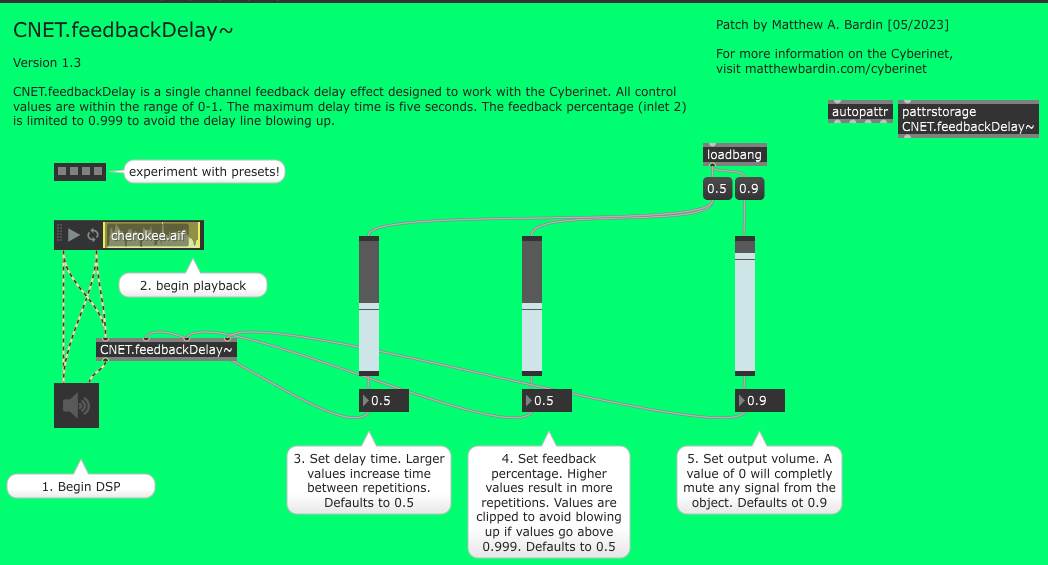
\includegraphics[scale=0.6]{diagrams/maxPatches/compressorHelp.png}
    \caption{Help Patch for CNET.compressor$\sim$}
    \label{fig:compHelp1}
\end{figure}

\begin{figure}
    \centering
    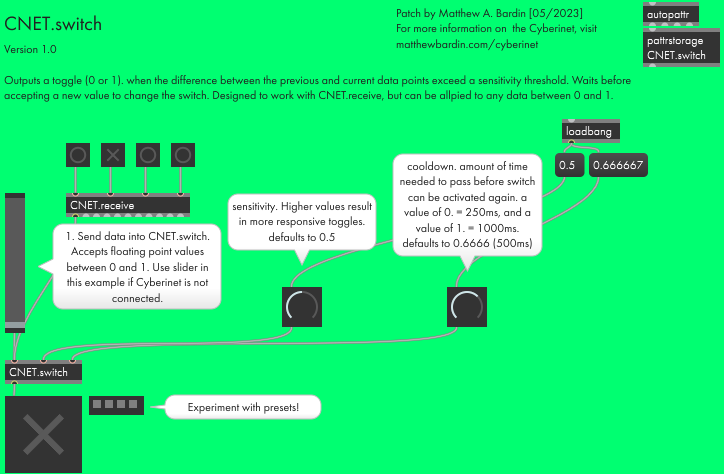
\includegraphics{diagrams/maxPatches/switchHelp.png}
    \caption{Help Patch for CNET.switch}
    \label{fig:switchHelp1}
\end{figure}

In addition to walking the user through how to setup and utilize the CNET object, each help patch contains between four and eight different presets. These are intended to show a variety of different parameter combinations, which reflect the capabilities of the object when used with the Cyberinet. Unless CNET.receive is required for the control object, it is not necessary to connect a Cyberinet to the computer in order to experiment with the help patches and their presets. Help objects where a physical Cyberinet connection is required are: CNET.receive, CNET.record$\sim$, CNET.rangeSet, CNET.test, and CNET.latency.


\chapter{Performing with the Cyberinet}
Now that we have looked into Every detail about how the Cyberinet was created and how to utilize its various features, let us take a moment to see how the Cyberinet is intended to be used. This is not an extensive list of all potential uses, but rather how I imagined the Cyberinet being useful to the various people who would want to utilize the instrument.


\section{Composition Tool}
One of the three main intended uses of the Cyberinet is as a compositional tool. Effectively, treating the Cyberinet as a completely new instrument or an add-on to a traditional B-flat clarinet. The flexibility of utilizing the Cyberinet's sensor data can result in a large variety of potential sounds, even without the need for the clarinet to make sounds. A performer can utilize multiple Cyberinet sensors without traditionally playing the instrument, allowing the composer to explore new performance routes.

The cybernetic capabilities of the Cyberinet also allow for experimentation with the interplay between the acoustic performance and the electronic components. The modularity of the sensor routing within Max and the choice of expansion sensors also help to increase the creative sound possibilities.\footnote{Early versions of the Cyberinet are intended to focus more on the alteration of the clarinet sound and controlling the Max environment, but more experimental developments are planned following the initial release.} The compositions discussed in Chapter 5 all focus on the variety of creative possibilities with the Cyberinet. 

Discussed in more detail in Chapter 5, each composition features a different utilization of the sensors. \textit{Puzzle of a Park} utilizes the button expansion to control a Max patch. The end result is similar to a loop pedal. \textit{Ethereal Presence} utilizes accelerometer data to control harmonization and backing noise. \textit{Raindrops on a Tin Roof} utilizes all of the available sensors in version 1.3 to trigger sound file play back, processing of live and recorded sounds, and live lighting changes.

When mapping the gesture data, a composer is able to define specific movements to occur at specific moments within a performance. However, as explained by Kvifte and Jensenius, it is important to consider the perspective of the listener\cite{KvifteJenseniusDescription}. From this perspective, the listener will identify a gesture and the resultant musical sound. This will happen regardless of if the identifies gestures are actually creating the sound. in a 2005 study, Wanderley et. al have found that:

\begin{quote}
    ... clarinetists' ancillary gestures are not randomly produced or just a visual effect, but rather they are an integral part of the performance process\cite{wanderleyClarinetGesture2005}.
\end{quote}

The Cyberinet functions by taking these generally ancillary gestures, and translate them into the realm of audibility. In order to translate this clearly, the parameters must be clearly described to the performer with a much greater level of specificity than would be needed than if describing it to a listener\cite{KvifteJenseniusDescription}. Using Kvifte and Jensenius' paper as a methodology for describing these gestures again, The Cyberinet exists squarely within the ratio level of measurement. This level of data is measured, with the distance of values determined, and an absolute zero value for each data exists, allowing for there to be 0 movement or airflow in the system. Being composed of specific values between 0 and 1, the data collected from the Cyberinet serves as a discrete input to the Max objects. Because of the modularity in the output, the sound production can be either continuous or discrete.

In practice, this results in a need for specificity in gesture notation to fully take advantage of the Cyberinet. A score needs to explain what, how, and when to perform certain gestures like those indicated within the previous chapter, as well as what the intended effect is\footnote{Chapter 5 will discuss how this was done or intentionally avoided, and how effective this was in practice.}. Mappings can be static, where a gesture will remain fixed to a specific parameter. Variable mappings can be changed by the performer either as instructed or in a improvisation manner. Another option discussed by Kvifte and Jensenius is the system being able to learn and modify itself based on the gestures of the performer\cite{KvifteJenseniusDescription}. While highly cybernetic in concept, the works discussed in Chapter 5 do not utilize this method of mapping.

As a final note on specifying the gesture mapping, It is recommended to avoid mapping multiple gestures and sensors to a single effect at one time. This can easily obscure what the listener is perceiving as the gesture, leading to an ambiguous relationship. However, having multiple effects controlled by a single gesture is less problematic as it can create a more complex musical result to an initial gesture.


\section{New Instrument}

As mentioned, the Cyberinet is intended as a new tool for the composer, but what about the performer? The Cyberinet straddles a line between new and old. It works to bring new sounds and functionality to a traditional instrument with its own performance practice. While the initial performances of the Cyberinet are intended to straddle this line, that is not all it can be. My ultimate goal is to treat the Cyberinet as its own unique instrument. Speaking purely practically, this brings about a certain mindset in the composer and performer when creating new music. I want the users to create music with the electronic features in mind, rather than working for an acoustic clarinet with additional aspects added. In writing the original compositions, the allowed for a more intentional integration of the motion and breath sensors, which resulted in clearer, more dramatic effects in performance.

As mentioned by Reid in regards to the MIGSI trumpet, creating a new computer-augmented instrument brings various elements to the forefront of the creation procession that would not normally be of concern. Specifically latency\cite{reid_2019}. When designing the Cyberinet, it was necessary to separate the instant audio response of the clarinet base from the electronic sound alterations and productions, which have a comparatively large amount of latency. The specific patch and process used to calculate latency is discussed in Chapter 3, and the measured average latency of the Cyberinet is PUT TIME IN HERE.

\section{Improvisation Tool}
% a la stomp boxes
Straddling the line between composer and performer brings us to the final, performance-based intended use for the Cyberinet: an improvisation tool. While mainly intended as a compositional tool, the Cyberinet leads to a large amount of exploration and improvisation. A few audio effects are provided with the Cyberinet to allow for the user to easily begin creating their own sounds, however the system can easily send its data to any object within the Max environment. By exploring which sensors are connected to different audio effects, the performer can create a large number of sounds based on a single performance movement that they are already used to. The large variety of options are discussed earlier in this chapter.

This modularity in signal processing is similar to the practice of using guitar stomp boxes to make a unique sound. While not physically similar, both systems allow for the quick customizable alteration of the instrument sound. When designing the available software objects, effects present in effect pedals such as reverb, delay, filters, and tuners were used as an inspiration. From a pure performance standpoint, the Cyberinet can be utilized to significantly reduce the amount of equipment needed. The goal of this is to free up the performer and allow them to be able to improvise and create new sounds more freely, without the need to consciously manage equipment.

\section{Educational Tool}
Admittedly, at the time of writing the idea of utilizing the Cyberinet as an educational tool is the least concretely defined idea discussed in this chapter. The concept came about when discussing the Cyberinet with various performers and graduate students during the LSU 2023 College of Music \& Dramatic Arts Research Expo. While not initially conceived in this manner, I feel that implementing the Cyberinet as an educational tool can have interesting and long-reaching results for future clarinetists and electro-acoustic music performances. 

In short, these discussions focused on the gyroscope (MPU-6050) and differential airflow pressure (SDP-31) embedded sensors. Looking at the gyroscope, the ability to determine the instrument's position could prove useful for new students learning the correct performance posture. This was the consensus of the small group of graduate researchers at the aforementioned event. I felt that bringing up the gyroscope in early education may have a unique side effect that was not brought up in the casual discussion, that being a potential to apply Cybernetic or Deep Listening concepts to a performer's mindset from an early age.

If a performer is able to see clearly on a screen what their current position is and how to change that to improve their sound and posture, then they are learning how to observe and analyze their body and make changes to the system in real-time; creating a Cybernetic feedback loop\cite{WeinerCybernetics2019}. While beyond the scope of this document, this action brings to mind several concepts of the Alexander Technique\footnote{For more information on the principals of the Alexander Technique, visit \url{alexandertechnique.com}}. Specifically, the concept of self-awareness and adjustments to free the performer from habitual problems\cite{gelbBodyLearning2013}.

It was with this context of seeing and learning to be aware of the air pressure that the conversation led into the use of the SDP-31 in an educational sense. By giving real-time numerical feedback a performer could learn what values to expect when performing at various volumes, the maximum and minimum amount of pressure difference they are able to create, as well as potentially identify any potential holes in their embouchure or leaky pads on their instrument. The same level of Cybernetic awareness and feedback apply to this sensor as well.

As additional expansions are created for the Cyberinet, their potential use in a pedagogical environment will need to be evaluated. Several of the expansions discussed in Chapter 2 have potential for educational use, and more could be created following appropriate design and market research.

\chapter{Music Works Written for the Cyberinet}

In addition to creating the hardware and software for this dissertation, I have also created a handful of musical compositions that show off various features of the Cyberinet. These four compositions as listed below, show a gradient from simpler to more complex uses of the Cyberinet’s features. Each piece's accompanying Max patch was given a unique color to make it easily identifiable to whoever is using the software. Full musical scores for each work are provided in Appendix C.

After looking at the compositions in detail, I want to explore what it is like performing with the Cyberinet through an interview with the premiere artist for all three of the works mentioned in this chapter\footnote{The scores for all pieces discussed in this chapter are available in the appendices and online at \url{matthewbardin.com}}.

\subsection{Notation Conventions}

As previously mentioned, the need for specific gestures is a necessity for the creation of meaningful Augmented Instrument functionality, and for the performer to be able to Cybernetically perform. Without these, the Cyberinet's software mapping becomes harder to define in a consistent manner\footnote{I am speaking from experience in this claim. The initial performance of the music happened prior to properly defining these elements, and ultimately resulted in more of a learning experience, rather than a musical demonstration.}. Towards this, I have utilized a small collection of gesture indicators within each of the musical scores. The analysis, testing and applications of gesture notation however, are outside of the scope of this paper. These symbols are intended to clearly indicate a type of movement or action, and are explained in detail in the score front matter. Following the finalization of the Cyberinet system, exploring an effective gesture notation for the instrument would prove both an interesting and fruitful course of study. In lieu of this, performers of the Music discussed in this chapter were asked their opinions on the notation in Chapter 5.5. The remainder of this subsection however will discuss the specific graphics used in the scores here, and not a potential list for every gesture mentioned by Wanderley et. al in figure \ref{tab:generalGestures}.


\subsubsection{Movement Indicators}
Four different movement indicators were given for the works discussed in Chapter 5. A variety was chosen in order to compare their effectiveness as a miniature experiment for future scores and studies. These include: 

\begin{itemize}
    \item Horizontal movement
    \item Vertical movement
    \item Rotation of the instrument
    \item Bobbing of the instrument
\end{itemize}

The horizontal movement indicator is the simplest of the four, and is comprised of a dashed horizontal line with an arrow on each endpoint. As used, this graphic indicates that the performer should intentionally exaggerate their horizontal movements for the sections of music underneath this line. For the performances discussed here, the gesture was back-and-forth movement, but this symbol can be easily specified by indicating direction with changes to the arrowheads and speed indicators.

\begin{figure}
    \centering
    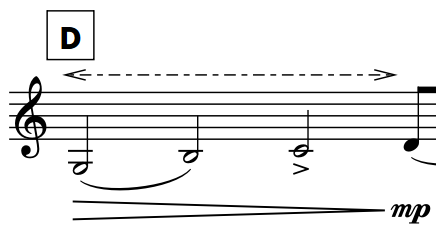
\includegraphics{Scores/horizontal.png}
    \caption{Horizontal Movement Indicator}
    \label{fig:horMovement}
\end{figure}

The vertical movement indicator may seem strange at first glance, but because I was again using a back-and-forth movement, I knew I wanted to utilize a graphic that emphasized this. I ultimately chose the one utilized in figure \ref{fig:vertMovement} because I felt it both did this, and sub-textually communicated a level of horizontal movement into the gesture. This is because incorporating smaller horizontal movement into large vertical movements is both natural and expressive. Simply moving the horn up and down would both look abnormal, and be uncomfortable for the performer. For these scores, the gesture should begin when the symbol first appears, then continue for the duration of that note, plus the duration of any tied or slurred notes. The gesture should stop when a rest or new articulation occurs.

\begin{figure}
    \centering
    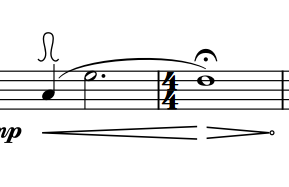
\includegraphics{Scores/wave.png}
    \caption{Vertical Movement Indicator}
    \label{fig:vertMovement}
\end{figure}

The final gesture essentially combines the previous two, resulting in a small vertical bobbing of the instrument while also moving the bell horizontally back-and-forth.


The symbol shown in figure \ref{fig:rotateMovement} is utilized differently than the others in this section. Generally speaking, the sensors are constantly applying the effects to an audio process for the others, but because of the coding of CNET.receive, the values are almost zeroed out unless the sensor values are actively changing. This is why indicators for the gestures are given: to show the sonic intentions of the composers for that section of music. The rotation gesture was utilized with CNET.switch, and only detected when the gesture occurred. This symbol indicates rotating the instrument with the wrist. This movement does not change the orientation of the Cyberinet to the player. I personally preformed it by holding the instrument with my left wrist, and quickly flicking that wrist away from my body then back into playing position.

\begin{figure}
    \centering
    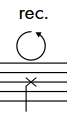
\includegraphics[scale=1.3]{Scores/trigger.png}
    \caption{Rotational Movement Indicator}
    \label{fig:rotateMovement}
\end{figure}


%%%%%%%%%%%%%%%%
% Need new graphic for the bobbing effect still
%%%%%%%%%%%%%%%%


\section{Puzzle of a Park}
At its core, this work is the simplest of the three written especially for this project. \textit{Puzzle of a Park} functions as a work written for a loop pedal, but without the pedal. The performer plays through the material from beginning to end, periodically pressing one of the two buttons on the button board accessory. Looking at the max patch we can see that one button will trigger the computer to record a microphone input into a buffer and triggers the synchronized playback of all recorded buffers, resulting in the loop pedal effect. The rotation gesture mentioned previously was also programmed to achieve this goal in case a user does not have the Button Expansion.

\begin{figure}
    \centering
    \includegraphics[scale=0.2]{diagrams/maxPatches/puzzlePresentation.jpg}
    \caption{\textit{Puzzle of a Park} Max Patch Performer View}
    \label{fig:puzzlePatchPres}
\end{figure}

\begin{figure}
    \centering
    \includegraphics[scale=0.25]{diagrams/maxPatches/puzzleRaw.jpg}
    \caption{\textit{Puzzle of a Park} Max Patch Full View}
    \label{fig:puzzlePatchRaw}
\end{figure}

This functionality allows for multiple recordings to be saved and layered, much like loop pedals such as the Boss RC line of pedals.

When writing this work, I viewed the musical content as a quartet, with four unique voices rather than a single voice repeated several times. This allowed the musical content to flow and feel more organic once the final layer was added. Once I had completed the short musical section, it was simply a matter of repeating the sequence of time signature and meter changes so that the score would form a repeating pattern. From there I had to decide exactly how to organize the various parts in time. Because I wanted this to be the simplest of the works in terms of performance and programming, I refrained from breaking down the recordings into smaller chunks and assembling them in Max. Instead, I choose the loop pedal approach and had the performer play through each voice before starting the playback and recording for the following voice. 

When ordering the voices, I began with one of the middle voices as the opening to the solo part. When comparing the voices in the score, these helped to provide a large amount of the background and a steady, albeit syncopated, pulse to the music. Something that helps to give the following bass voice more context during the measures where it is simply holding a pedal tone during the second section. Looking at the large-scale musical form of the solo, I would describe it as \emph{ABA'C} since the third and first voice are often coordinated, providing harmonic content. I viewed them like a horn part in a Sousa march in this regard. When combined, the first three voices provide a complete backing track to the main melodic line. Like fitting together, the pieces of a puzzle, it is this final line that helps to give context to all the phrases we have heard so far. Down beats become upbeats, harmonic implications shift with the addition of new chord tones, and the texture is filled out to include the full range of the instrument.

When it came to gesture mapping, this piece utilizes the least of the works discussed in this chapter. In testing, it became a concern that the playback could potentially overpower the performer, so to mitigate that, the data from the air flow sensor was inversely mapped and applied to the make up gain parameter of CNET.compressor$\sim$, which all recorded sound files are sent through. This resulted in the make up gain level decreasing as the performer played more loudly. In general, this kept all four parts in relative balance, but would occasionally dip too much when the line was naturally louder.

The second effect is built out of a previous object I created as part of the emdm Max collection. This effect takes an incoming audio signal, analyzes its frequency compositing, and then filters noise at a low volume to result in a constantly shifting background sound that will always match the performance. When vertical movement is occurring, the sounds form this effect are mixed into the output, adding an additional level of texture to the performance.

\textit{Puzzle of a Park} was premiered by Adam Cope on 04/18/23 at the LSU Digital Media Center Theatre and recorded approximately a month later.

\section{Ethereal Presence}
Ethereal Presence is the second work created for this project begins to utilize the more complicated sensors present in the Cyberinet. The specified gestures all utilize the various movement sensors. Once received, the Max patch for the composition utilizes the values to control two different synthesizers and their parameters, listed in figure \ref{fig:etherealSynths}. 

\begin{figure}
    \centering
\begin{itemize}
    \item Pitch-shifted FM Synthesis that harmonize with the original clarinet sound based on the vertical movement of the performer.
    \item Filtered pink noise using FFT bins that respond to the Horizontal position of the performer.
\end{itemize}
    \caption{Synthesizers used in Ethereal Presence}
    \label{fig:etherealSynths}
\end{figure}

The rotation gesture was used to change the active sensor depending on the section of music.

The first synthesizer Is a simple FM synthesizer with the goal of harmonizing with the soloist, and is the titular "Ethereal Presence". The goal is to make the tone as simple as possible, but with a large potential for timbral changes. The pitch of the incoming microphone signal is analyzed using CNET.pitchShift$\sim$, which is used to determine the pitch of the FM synthesizer. The pitch will increase was the performer moves vertically, and decrease as they move downward. Little or no Movement will result in the FM synthesis matching the performer.

% Cite Austin's Dissertation in this paragraph
Accompanied by this is a more textural synthesizer designed to help support and fill out the atmosphere of the composition. This synthesizer outputs noise before being run through an FFT based filter created by Dr. Austin Franklin. This filter takes the incoming noise and performs an FFT operation on it to determine the frequency content, then based on the values received from the Cyberinet, filters out certain frequency bins. The end result is a fluctuating cloud of noise that adapts its frequency range based on the Cyberinet's position. The range will increase with leftward movement, and decreases when moving to the right.


\begin{figure}
    \centering
    \includegraphics{diagrams/maxPatches/ethereal_pres.png}
    \caption{Ethereal Presence Performer View}
    \label{fig:etherealPerf}
\end{figure}

\begin{figure}
    \centering
    \includegraphics[scale=0.75]{diagrams/maxPatches/ethereal_raw.png}
    \caption{Ethereal Presence Full View}
    \label{fig:etherealRaw}
\end{figure}

When mapping gestures, all but the structural rotation gestures are listed as "optoinal, but highly encouraged" Aesthetically, I want no two performances will harmonize in the exact same way each time, thus increasing the "etherealness" of the effect. The indicated gestures are how I imagined the sounds when writing the work, but I also wish for the performer to experiment and find their own placement of the gestures based on their own unique tastes. The specific gestures being monitored cannot be changed without reprogramming the Max patch, so the main experimental factors are the timing of the gestures, and the size of the movements.

In practice, I found that I would have preferred to have even more specific motions indicated in the score, even if they are kept optional or otherwise indeterminate. While the performers I have shown this to have indeed all performed with exaggerated expressive movements, everyone\footnote{I showed the score to a total of three different performers outside of preparations for the premiere.} was only moving at about 50-80\% of the maximum effect range, and had to be encouraged to further exaggerate their movement to hear the full effect. I feel that by indicating with more specificity as laid out in the previous chapter would help performers to more easily understand to what degree of motion they need to move to work with the Cyberinet. 

Because every performer is different and may be unable to achieve the full range of gestures, a max object, CNET.rangeSet, was created to help mitigate that problem. CNET.rangeSet can adjust the scaling parameters within CNET.receive in order to make the results more or less sensitive. A smaller movement can result in a larger change in effects. It is recommended that this be utilized for calibration if an effect is not coming through as desired.


\textit{Ethereal Presence} was premiered by Adam Cope on 04/18/23 at the LSU Digital Media Center Theatre, and recorded later that summer.

\section{Raindrops on a Tin Roof}
Of the three debut compositions for the Cyberinet, \textit{Raindrops on a Tin Roof}\footnote{A performance video of \textit{Raindrops on a Tin Roof} is available at} is the most involved with the Cyberinet sensors. Contrasting from Mueller's usage of the SABRe, this composition utilizes all of the default sensors present in the hardware in some way. 

The inspiration comes from a short story I wrote in late 2022. The full text is provided in the appendices, but the general outline is as follows:

The main character is exhausted after a week of overtime at work and plans to enjoy a rainy weekend alone at home. during the storm, the protagonist falls asleep and wakes up to find the house completely dark and unfamiliar. Assuming the power has just cut out, they head to the basement to find some emergency lights when they discover an un-knowable eldritch abomination in the basement. Because of the un-knowable nature of the being, the protagonist forgets everything about it as soon as they run away. The end result is a bloodthirsty monster chasing the protagonist through the house and onto a rooftop veranda where the protagonist accepts their fate, and the monster has its dinner.

Formally, the music follows the narrative of the story, with ambient storm sounds and monster noises coming in as indicated. 

Gyroscopic information is used to control the live mixing of the pre-rendered tracks. These include:
\begin{itemize}
    \item Sounds created by the monster.
    \item Creaking floorboards and other ambience.
    \item Synthesizer Accompaniment.
    \item Narrator readings.
\end{itemize}

The gyroscopic information is also used to alter effects applied to all of the aforementioned sounds as well as the clarinet. This is combined with the accelerometer information to avoid having the correlation become predictable.

The airflow information is used to apply distortion and other processing to the audio signals. In short as the performer's breathing increases, so does the effect application.

Unlike the other compositions discussed here, \textit{Raindrops} utilizes notated accompaniment. This accompaniment is meant to represent the monster in the basement in a less literal sense. For the premiere, these sounds are generated with the UVI 8-Bit Synth. The sounds were all pre-rendered using Studio One 6 Professional, and are intended to create a spooky, slightly incongruous sound when compared to the other sounds in the environment. 

The narrator files are a processed recording of the composer reading the story. the processing adds a distorted, low-fi sound to the voice to make it appear more ethereal in nature than the clean recordings. 

The final two non-musical elements of this performance are a smoke machine and at least 2 DMX-controlled lights. The smoke machine is not controlled by the performer, but the DMX lights are. The RGB lights are controlled by a mix of gyroscope and airflow values. The end result is the lights changing as he performer moves around the stage, and becomes more red as the performer breathes harder.

\begin{figure}
    \centering
    \includegraphics{diagrams/maxPatches/raindropspres.png}
    \caption{Raindrops on a Tin Roof Performer View}
    \label{fig:raindropsPres}
\end{figure}

\begin{figure}
    \centering
    \includegraphics[scale=0.6]{diagrams/maxPatches/raindropsRaw.png}
    \caption{Raindrops on a Tin Roof Full View}
    \label{fig:raindropsRaw}
\end{figure}

When mapping gestures, the score for \textit{Raindrops on a Tin Roof} contains the most specific level of gesture notation. In general, three gestures are utilized outside of the natural gestures of a performance. These are: 

\begin{itemize}
    \item Exaggerated movement
    \item Exaggerated breathing
    \item Movement between stands on stage
\end{itemize}

When notating this work, one concern was clutter on the page. to help minimize this, the score was printed on tabloid (11inx17in) sized paper\footnote{The score has been scaled down to fit within this document.} in order have more physical space on the page. Because of the large amount of narrator text in this work, the text indication was given as boxed text, indicating the first and last line of the clip, as well as the clip's duration. Two symbols were used to indicate the exaggerated movement and breathing. The first, being a looping line, was intended to indicate exaggerated movement of the Cyberinet. This proved effective as the shape led the performer to naturally move in a looping motion and trigger the effect. The zig-zag shape was included to represent exaggerated breathing in a section. This came through less clearly, but was easily adjusted with CNET.rangeSet.

The final gesture indicator was to move to a different location on the stage. This was indicated with text at the appropriate place on the score. No physical transitions occurred before the end of a page, and this proved effective is sending a large number of values to all of the sensors at once, resulting in a more drastic effect to mirror th physical movement. An exploration into the gesture mapping notation is intended for further refinement.

\textit{Raindrops on a Tin Roof} was premiered by Adam Cope on 04/18/23 at the LSU Digital Media Center Theatre, but did not include the optional smoke machine.

\section{ImprovImpisaImptionImpprovisation in Reverb}
Similarly to \textit{Ethereal Presence}, \textit{ImprovImpisaImptionImpprovisation in Reverb} utilizes the gyroscope and accelerometer to control the computer processing. However instead of using the sensor data to control audio synthesis, this composition's algorithm controls multiple reverb and delay effects applied to the incoming signal from an onstage microphone.

\begin{figure}
    \centering
    \includegraphics{diagrams/maxPatches/imporvPres.png}
    \caption{ImprovImpisaImptionImpprovisation in Reverb Performer View}
    \label{fig:ImprovPres}
\end{figure}

\begin{figure}
    \centering
    \includegraphics{diagrams/maxPatches/improvRaw.png}
    \caption{ImprovImpisaImptionImpprovisation in Reverb Full View}
    \label{fig:improvFull}
\end{figure}

The specific control mapping for this composition are as follows: 

\begin{itemize}
    \item GyroX: gates signal to CNET.feedbackDelay$\sim$
    \item GyroY: feedback delay time
    \item AccelX: feedback delay percentage and output gain, and low harmonizer pitch
    \item AccelY: high harmonizer pitch
\end{itemize}

Of the four compositions discussed in this chapter, \textit{ImprovImpisaImptionImpprovisation in Reverb} is the only one that does not have a dedicated score. This was done to focus on the potential use of the Cyberinet as an improvisation tool. By utilizing the movement data from the Cyberinet, the patch encourages the performer to explore the performance space. In terms of the physical movements required to trigger the effects, they are closest to those used in \textit{Ethereal Presence}. All of the mapping comments discussed in the section regarding \textit{Ethereal Presence} apply to this work as well, however are less potentially problematic due to the implicit experimentation and response nature of improvisation. Sensor value mappings are given in the max patch, but without a score, it proves difficult to notate specific gestures.

The max patch for this composition contains three main processes controlled by the Cyberinet. The first is a reverb effect that is constantly applied to the sound. The amount of reverb present changed based on the horizontal movement of the performer. Following that, the patch automatically swaps between two different states. The first is a feedback delay where the delay time is controlled again by horizontal movement. Specifically, the audio signal for this process is only fed into the delay line when the instrument has been shaken or is otherwise actively moving horizontally. The final state of the patch takes the signal and using CNET.tuner$\sim$ and CNET.pitchshift$\sim$, creates triangle waves that harmonize above and below the performer based on their Y-axis movement (upstage vs downstage). These states alter randomly for the duration of the performance, and are fed into additional, non-automated reverb effects as well as a patch which generates low-level background noise based on what is happening in the pitch-space of patch. If desired, the performer can utilize one of the buttons from the button expansion in order to both mute the sounds in an emergency, as well as manually swap between the mapping states.

This max patch utilizes a slightly different version of CNET.receive. This one is called CNET.receiveCaps. It is completely identical to CNET.receive in every way except that the labels used to route the sensor data all begin with capital letters. Because of the similarity with CNET.receive, this object is not discusses separately. It exists because the Cyberinet hardware used in the premiere of this work utilized an older version of the Arduino code that used capital letters instead of the camel-case that is conventional to modern coding. All versions of the Cyberinet following 1.2 use the preferred camel-case.

While not complex, this work emphasizes Van Nort's idea of a second-order level of gesture mapping\cite{vanNortMapping2007}. By being able to automatically or manually swap between the mapping states, the performer is able to further control and develop the relationship between sound and action. In a performance, the max patch will always default to the first state: the feedback delay. By having to move the instrument horizontally to activate the effect, the intention is that the listener will see the clear relationship between the two actions. Then, while not as drastic of an effect, the horizontal movement is utilized in the harmonization effect. The main control for the harmonizer is leaning back. Combined with a reverb effect that is always being affected by horizontal movement to act as an acoustic and gestural glue, the performer is able to create a clear relationship between the sounds and develop subtle variations between that relationship in a performance setting. I look forward to seeing future expansion on the idea of Second-Order gesture control with the Cyberinet in future compositions.

\textit{ImprovImpisaImptionImpprovisation in Reverb} was premiered on 05/01/2023 by Matthew A. Bardin in the LSU School of Music Recital Hall.

\chapter{Conclusions} % better title? can be last thing.

\section{User Opinions}

As previously stated, being a new augmented instrument, the aforementioned four works are the only compositions for the Cyberinet at the time of writing. To better inform future revisions and compositions, the two performers who premiered the above works were asked a series of questions following their usage of the Cyberinet. These questions were:

\begin{itemize}
    \item Question 1: How easy or difficult was it to implement the Cyberinet into your normal performance routine?
    \item Question 2: What was your favorite and least favorite part about working with the Cyberinet? 
    \item Question 3: How confident do you feel in being able to remove or add the Cyberinet to your clarinet in a performance setting?
    \item Question 4: How confident do you feel in being able to work with the Cyberinet's software capabilities to create unique sounds?
    \item Question 5: What thing or things did you dislike, or would change, about the Cyberinet?
\end{itemize}

In order to protect the identity of the performers, they are referred to by number. Performer 1's responses are shown below: % Adam

\begin{itemize}
    \item A1: It's very straightforward, akin to switching clarinets, as one would for an orchestra performance. Just switching out the barrel and adding the thumb rest attachment it all it takes to incorporate the Cyberinet into my performance routine.
    \item A2: My favorite part about working with the Cyberinet has been exploring how to incorporate the movement sensors into my performance. Normally the way you move doesn't directly affect the sound you're putting out, so it's interesting to see the new ways in which I can express myself! My least favorite part is probably th
    \item A3: Assuming future versions will be able to connect and transmit data more reliably, I would say I'm very confident in adding and removing the Cyberinet.
    \item A4: As someone who is not well versed in Max, I'm not confident in my ability to create new sounds on the software side of things. As a performer first, I feel confident in my ability to use the equipment, but not necessarily to create for it.
    \item A5: The only thing I would change is to reverse the ports that connect the thumb rest buttons to the barrel. Right now, the connecting cable kind of sticks into the player's right hand a bit, but I imagine that would be a non issue if the ports were flipped to the opposite side.
\end{itemize}


The below responses belong to performer 2. % Me

\begin{itemize}
    \item A1: It was simple enough to implement, however there was a bit of a learning curve needed to reliably connect the device to the computer. Once I had the steps memorized it was reliable and simple to use.
    \item A2: My least favorite part was having to install all of the various drivers the first time. My favorite part was exploring with the gyroscope sensor and a reverb effect. the result was fun and intuitive.
    \item A3: I've already mentioned the issues in setting up the Cyberinet at the beginning, but being able to simply turn off the power and utilize the instrument completely acoustically as needed. This is easier than removing the unit.
    \item A4: I am already familiar with the Max environment so I feel that I could easily set up a lot of scenarios with the Cyberinet without much difficulties, but more reference material would be helpful. 
    \item A5: Other than the things I've already mentioned, I suppose I'd say relocating the port on the Button Expansion to a better location and potentially reducing the size of the main unit a little. It isn't too large, but a think a little smaller would be easier to work with.
\end{itemize}

In general, the people using the Cyberinet find it easy to implement both in terms of hardware and software, but mainly request various tweaks to different aspects of the design. Since these questions have been asked, the thumb rest has been altered to resolve this problem and the Max objects have also been optimized for simpler connections and management, but other improvements will have to wait until the second iteration.

\section{Future Development}

In the current software version, the button LED's are only illuminated when the buttons are pressed. However they are wired independently of the switches on the expansion. In future versions, the ability to control these LED's via the software is planned.


At the time of writing, the Cyberinet is only available for B-flat soprano Clarinets. While this is the most commonly found Clarinet, it represents only a fraction of the total woodwind family. In the future, plans to adapt the hardware case to fit different instruments will allow for the Cyberinet to be utilized in an exponentially larger number of scenarios. 

First, adapting the unit for the A Clarinet and Bass Clarinets. At this time there are no plans to expand to an E-flat Clarinet due to the limited space to attach electronic components. Following the Clarinet expansions, ideas for compatibility with Saxophones and Flutes are being discussed, but require more planning in order to make functional units.

Outside of the aforementioned hardware needed to make the Cyberinet framework compatible with more instruments, improvements to the cable stress relief, and an increase in modular expansions is also planned. Initially only additional buttons available, but the aforementioned joystick and microphone expansions will be completed over the summer and fall of 2023. Additional plans for the following sensors to be released following those have also been made, but active development has not yet begun at the time of writing.

\begin{itemize}
    \item Pressure Sensor: responds to varying pressure on the instrument's keys. Needs special mounting of Force-Sensitive-Resistors, as well as doughnut-shaped FSRs.
    \item Pitch Detection: Works like the tuner software object. This will display tuning information and transmit pitch information to the computer. Needs hardware with adequate Analog-to-Digital Conversion.
\end{itemize}



Potential freeware software options such as Pure Data are being considered, but at the time of writing, are not in active development.

Plans for the expansion and revision of the software environment are already underway. Future goals include:

\begin{itemize}
    \item Adapt messages to OSC formatting for a greater range of software compatibility.
    \item OS compatibility: Version one of  the Cyberinet currently only works on MacOS devices. Future plans involve compatibility with Windows devices as well.
    \item Increasing Effects: Expanding for additional audio effects. Plans include filters, synthesizers, and automatic harmonizers.
    \item Max Library: Once expanded and revised, Plans to reach out to Cycling74 to have this collection of Max objects listed in the program as an available-for-download library will be made. This will make it simpler for people to access various tools for their Cyberinet unit.
    \item Standalone Software: The final planned software expansion for version one is to take the Max environment and export it as a standalone software. This will allow for the user to access the tools and capabilities of the Cyberinet without needing Max, which can be a financial hindrance to some people.
\end{itemize}

\section{Conclusions}




%% The command ``\appendix'' switches into appendix-mode, meaning that subsequent ``\chapter'' commands will instead produce appendices.
\appendix

\chapter{Cyberinet Hardware Designs}
This appendix contains images for all of the 3D models and PCBs used within the Cyberinet. It also contains close-up images of each of the individual OEM sensors.

\section{3D models}
Below are all of the 3D models utilized to 3d print the case and accessories of the Cyberinet

\subsection{Main Body}

\begin{figure}
    \centering
    \includegraphics[scale=0.4]{diagrams/3D Models/Cyberinet main case 3d.png}
    \caption{Main Unit of the Cyberinet from various angles}
    \label{fig:main3D}
\end{figure}



\subsection{Button Board Thumbrest Mount}

\begin{figure}
    \centering
    \includegraphics[scale=0.8]{diagrams/3D Models/thumbrestPic.png}
    \caption{Button Board Thumbrest Mount in 3D printing software}
    \label{fig:thumbrest}
\end{figure}



\section{PCB Diagrams}
Below are the PCB diagrams for the Cyberinet. Main unit and Button Expansion


\begin{center}
\begin{figure}
    \centering
    \includegraphics[scale=0.3]{diagrams/PCBs/mainBoard.png}
    \caption{Cyberinet Main Unit PCB}
    \label{fig:mainPCB}
\end{figure}
\end{center}



\chapter{Cyberinet Software Components}
This appendix contains all of the Arduino code flashed to the Cyberinet. (Version 1.3), as well as screenshots of the various max patches and objects included in the software bundle.

\section{Arduino .ino Code}

Below is the .ino code that is running on the ESP-32 micro-controller. This code was developed using the Arduino IDE and coding language.

\begin{lstlisting}[language=Arduino] 
/* Micro Controller Code for the Cyberinet Version 1.3, Code may be used or reworked with Attribution.
   Code and Other Matierials for the Cyberinet can be found at https://github.com/mbardin/Cyberinet
   Code and Other Marerials made  by Matthew A. Bardin [2023] (https://matthewbardin.com)*/

//libraries to include
#include <SparkFun_SDP3x_Arduino_Library.h>
#include<Wire.h>
#include <BluetoothSerial.h>
#include <MPU6050.h>

BluetoothSerial SerialBT;
MPU6050 mpu;
SDP3X airFlow;

const int pwrLED = 2; 
const int msgLED = 4; 
const int button1 = 12;
const int button2 = 14;
const int b1LED = 26;
const int b2LED = 27;
const int expPin1 = 33;
const int expPin2 = 32;
const int expPin3 = 35;
const int expPin4 = 18;
const int MPU_ADDR = 0x68; 
int16_t AcX, AcY, AcZ, GyX, GyY, GyZ; 
float rotX, rotY, rotZ, gForceX, gForceY, gForceZ; 
int button1State = 1;
int button2State = 1;
int exp1State = 0;
int exp2State = 0;
int exp3State = 0;
int exp4State = 0;

void setup() {

  pinMode(pwrLED, OUTPUT);
  pinMode(msgLED, OUTPUT);
  pinMode(button1, INPUT_PULLUP); 
  pinMode(button2, INPUT_PULLUP);
  Serial.begin(115200);
  SerialBT.begin("CyberinetV13"); 
  delay(1000); // pause before checking
  gyroStartup();
  airflowStartup();
  startLights();
}

void loop() {
  get6050();
  getButtons();
  getExp();
  getAir();
}

void get6050() {
  Wire.beginTransmission(MPU_ADDR);
  Wire.write(0x3B); 
  Wire.endTransmission(true);
  Wire.requestFrom(MPU_ADDR, 6); 
  while (Wire.available() < 6);
  AcX = Wire.read() << 8 | Wire.read(); 
  AcY = Wire.read() << 8 | Wire.read(); 
  AcZ = Wire.read() << 8 | Wire.read(); 
  Wire.beginTransmission(MPU_ADDR);
  Wire.write(0x43); 
  Wire.endTransmission();
  Wire.requestFrom(MPU_ADDR, 6); 
  while (Wire.available() < 6);
  GyX = Wire.read() << 8 | Wire.read();
  GyY = Wire.read() << 8 | Wire.read();
  GyZ = Wire.read() << 8 | Wire.read();
  rotX = GyX *  0.007633587786; 
  rotY = GyY *  0.007633587786;
  rotZ = GyZ *  0.007633587786;
  gForceX = AcX * 0.00006103515;
  gForceY = AcY * 0.00006103515;
  gForceZ = AcZ * 0.00006103515;
  digitalWrite(msgLED, HIGH); 
  SerialBT.print("gyroX "); 
  SerialBT.println(rotX); 
  SerialBT.print("gyroY "); 
  SerialBT.println(rotY); 
  SerialBT.print("gyroZ "); 
  SerialBT.println(rotZ);
  SerialBT.print("accelX ");
  SerialBT.println(gForceX);
  SerialBT.print("accelY ");
  SerialBT.println(gForceY);
  SerialBT.print("accelZ ");
  SerialBT.println(gForceZ);
  digitalWrite(msgLED, LOW);
}

void getButtons() {
  button1State = digitalRead(button1);
  button2State = digitalRead(button2);
  digitalWrite(msgLED, HIGH); 
  SerialBT.print("b1 ");
  SerialBT.println(button1State);
  digitalWrite(b1LED, button1State); 
  SerialBT.print("b2 ");
  SerialBT.println(button2State);
  digitalWrite(b1LED, button2State);
  digitalWrite(msgLED, LOW); 
}

void getExp() {
  exp1State = digitalRead(expPin1);
  exp2State = digitalRead(expPin2);
  exp3State = digitalRead(expPin3);
  exp4State = digitalRead(expPin4);
  digitalWrite(msgLED, HIGH);
  SerialBT.print("exp1 ");
  SerialBT.println(exp1State);
  SerialBT.print("exp2 ");
  SerialBT.println(exp2State);
  SerialBT.print("exp3 ");
  SerialBT.println(exp3State);
  SerialBT.print("exp4 ");
  SerialBT.println(exp4State);
  digitalWrite(msgLED, LOW);
}
void getAir() {
  float diffPressure; 
  float temperature; 
  airFlow.readMeasurement(&diffPressure, &temperature);
  digitalWrite(msgLED, HIGH); 
  SerialBT.print(F("airP ")); 
  SerialBT.println(diffPressure, 2); 
  SerialBT.print(F("temp "));
  SerialBT.println(temperature, 2);
  digitalWrite(msgLED, LOW); 
}
// startup functions
void gyroStartup() {
  Wire.begin(21, 22, 100000);
  Wire.beginTransmission(MPU_ADDR);
  Wire.write(0x6B); 
  Wire.write(0);     
  Wire.endTransmission(true);
  SerialBT.println("MPU-6050 Setup Complete");
}

void airflowStartup() {
airFlow.stopContinuousMeasurement();
 if (airFlow.begin() == false){
  SerialBT.println(F("SDP31 not detected.));
  while (1);
  }
airFlow.startContinuousMeasurement(true, true); 
SerialBT.println("SDP31 Setup Complete");
}

void startLights() { 
  digitalWrite(pwrLED, HIGH);
  digitalWrite(msgLED, HIGH);
  delay(500);
  digitalWrite(msgLED, LOW);
  delay(500);
  digitalWrite(msgLED, HIGH);
  delay(500);
  digitalWrite(msgLED, LOW);
  delay(1000);
  digitalWrite(msgLED, HIGH);
  delay(1000);
  digitalWrite(msgLED, LOW);
}
\end{lstlisting}


\section{CNET Max Objects}
This section discusses each of the CNET objects that were created with the intention of interfacing with the Cyberinet. With the exception of CNET.receive, these are smaller objects designed to easily implement the Cyberinet into some of the common audio effects the user is likely already implementing in Max. Because of how CNET.receive works, these objects are not required to utilize the Cyberinet, but are recommended for people learning how to work with Max or the Cyberinet for the first time.

Each object listed here also has a help patch which walks the user through setup and adjusting the values for that object. The help patches do not need the Cyberinet to be connected to work, and contain 3 different presets to show a variety of sound options. All inlets for these object utilize a 0-1 floating point number for parameter control. Default values for these inlets are all given in the help patches.

\subsection{Functional Objects}
These objects serve to increase the functionality of the Cyberinet and do not alter sound sources or control other objects.

\subsubsection{CNET.receive}
This is the only required object in the CNET collection. This object is responsible for setting up communications with the Cyberinet, parsing the data, and outputting it to the various outlets. Each sensor on the Cyberinet has a dedicated outlet, so connecting to each outlet will always relay the same sensor. The outlet order is given below.

\begin{enumerate}
    \item gyroX
    \item gyroY
    \item gyroZ
    \item accelX
    \item accelY
    \item accelZ
    \item b1
    \item b2
    \item airP
    \item temp
    \item exp
    \item errorMsg
\end{enumerate}

The final outlet will output an error indicating that CNET.receive received a message it did not recognize, as well as the error causing message.

To establish communications, bangs and toggles are utilized in order to simplify the interface. The user inputs a bang to the first inlet to start the script and list the available ports. When paired to the computer via Bluetooth, the Cyberinet will appear on the list of available ports. The user can then set the port by filling in the message box connected to inlet 2, and receive communications with a bang to the third inlet. Inlet 4 will stop all communications. The process will have to be repeated to initialize them again, and a bang to inlet 5 will install necessary node package manager dependencies and drivers the first time a computer is utilizing the Cyberinet.

The Node script and functionality comes from a package created by the LSU Experimental Music \& Digital Media department, and the JavaScript code for this is shown below in its entirety.

\begin{verbatim}
// EMDM Serial communications in Max
const path = require('path');
const Max = require('max-api');

const { SerialPort, ReadlineParser } = require('serialport')
const baud = 115200;
let devicePort = '/dev/tty-CyberinetV13'

// Create a port
let port;
let availablePorts;
let parser = new ReadlineParser();


Max.post(`Loaded the ${path.basename(__filename)} script`);

Max.addHandler("bang", () => {
	Max.post("Who you think you bangin'?");
});

Max.addHandler("echo", (msg) => {
	Max.outlet(msg);
});

Max.addHandler("portlist", () => {
  SerialPort.list().then((ports)=>{
    Max.post("Ports: ", ports);
    console.log(ports);
    availablePorts = ports;
  });
});

Max.addHandler('setPort', (port) => {
  devicePort = port;
})

Max.addHandler('open', () => {
  port = new SerialPort({
    path: devicePort,
    baudRate: baud,
  }, function (err) {
    if (err) {
      return console.log('Error: ', err.message)
    }
  })
})

Max.addHandler('enable', () => {
  Max.post('Serial Receive Enabled');

  port.pipe(parser)
  parser.on('data', (cyberData)=>{
    let cyber = cyberData.split(" ");
    let sensor = cyber[0];
    let value = parseFloat(cyber[1]);
    Max.outlet(sensor, value);
  })
})

Max.addHandler('send', (data) => {
  port.write(data, function(err) {
    if (err) {
      return console.log('Error on write: ', err.message)
    }
    console.log('message written')
  })
})
\end{verbatim}

In short, after setting up the port communications, this code will identify the label:value pair and output them separated by a space via the outlet in the Node object. From there, a Max route object separates the values to different outlets based on the labels shown above. Values are scaled to fit a range of 0-1 where appropriate.

\subsubsection{CNET.rangeSet}
Used for adjusting the value scaling within CNET.receive. This object is used to fine tune the ranges expected for a performer with their Cyberinet unit. Maximum and minimum sensor values can be determined by looking at the Max terminal when the raw outputs are being displayed. Ranges are set to a specific sensor utilizing the same labels as those used in CNET.receive. Setting the sensor label with a message or sending a bang to the first outlet will trigger a list to be output from this object.

Within CNET.receive, an additional route and a handful of unpack objects are used to properly apply the data. All values leaving CNET.receive are still mapped to a range of 0-1 after this new scaling occurs.

\begin{figure}
    \centering
    \includegraphics{diagrams/maxPatches/CNET.rangeSet.png}
    \caption{CNET.rangeSet.maxpat}
    \label{fig:CNET.rangeSet.maxpatch}
\end{figure}

\subsubsection{CNET.latency$\sim$}
Used to calculate the latency between the Cyberinet detecting a sensor value change on the hardware, and that change being reflected in the Max environment. To achieve this, a microphone is needed. 

To test the latency, first you must connect the Cyberinet using CNET.receive, and ensure that the Button expansion is connected. 

Using the patch, a sound file is recorded. One channel of the stereo file records the sound of a button clicking on the Cyberinet. This button press is used to generate a pulse of white noise on the second channel.

The recordings are then compared to determine the time between the real-world action and the software response which is represented in milliseconds for the user. Large objects located between the computer and the Cyberinet may negatively affect the latency.

\subsubsection{CNET.tuner$\sim$}

This object is a simple tuner based off of the retune$\sim$ object native to Max. It receives a signal from an external microphone and outputs both the closest MIDI pitch and frequency of the sound. These values are output as signals. In this version of the Cyberinet, it must be located in the Max software as the ESP-32's ADC's are not powerful enough to run a tuner along with everything else. It is recommended for both tuning purposes, as well as pitch identification purposes. 

\begin{figure}
    \centering
    \includegraphics[scale=0.2]{diagrams/maxPatches/CNET.tuner~.png}
    \caption{CNET.tuner$\sim$.maxpat}
    \label{fig:CNET.tuner~.maxpat}
\end{figure}
 

\subsubsection{CNET.click$\sim$}
This object is able to receive a BPM value and outputs both a bang in Max, but also sends an audio signal click. This signal can be used by connecting a [receive$\sim$ click] to the desired output. For the compositions discussed in this document, the click track was always connected to channel 3 of the audio interface.

\begin{figure}
    \centering
    \includegraphics[scale=0.2]{diagrams/maxPatches/CNET.click~.jpg}
    \caption{CNET.click$\sim$ max patch}
    \label{fig:CNET.clickPAtch}
\end{figure}

\subsubsection{CNET.pan}
I was unsure about which section to place this object in. I chose its ultimate placement here as the object is not directly changing the sound, but rather it receives data to control the stereo panning of a signal.

\subsubsection{CNET.dmx}
This object functions to allow the Cyberinet to control DMX lighting with its various sensors. Note that this will not work with every DMX controller, and is specifically designed to interface with the Chauvet DMX-AN 2. After being setup with the desired environmental settings, CNET.dmx takes in three sensor readings to control the red, green, and blue levels of the connected lights.

\begin{figure}
    \centering
    \includegraphics[scale=0.85]{diagrams/maxPatches/CNET.dmx.png}
    \caption{CNET.dmx.maxpat}
    \label{fig:CNET.dmx.maxpat}
\end{figure}

\subsection{Audio Effects}
These audio effects are designed to receive information from the functional objects above and utilize the data to either process sound or control another object. Generally, these effects are relatively simple alterations of sounds similar to audio effects found in most DAW's.

\subsubsection{CNET.reverb$\sim$}
This is a stereo Schroder reverb internally similar to the popular JC reverb developed by John Chowning. Type more here about the effect. Include how it works, the parameters that can be controlled, and anything unique about it. 

\begin{figure}
    \centering
    \includegraphics{diagrams/maxPatches/CNET.reverb~.png}
    \caption{CNET.reverb$\sim$.maxpat}
    \label{fig:my_label}
\end{figure}

\subsubsection{CNET.monoReverb$\sim$}
This patch is identical to CNET.reverb$\sim$, except that it outputs a mono signal instead of stereo.

\subsubsection{CNET.compressor$\sim$}
CNET.compressor is a fairly standard compressor that is able to receive data from the Cyberinet in order to control the threshold, ratio, attack, release, and gain staging before and after the effect. By connecting a meter$\sim$ object to the last outlet, a faux VU meter can be created to show the gain reduction happening in the compressor. One unique feature of this compressor is that it takes in a mono signal and outputs a stereo signal.

\begin{figure}
    \centering
    \includegraphics{diagrams/maxPatches/compInner.png}
    \caption{Inner workings of CNET.compressor~}
    \label{fig:compressor~Inner}
\end{figure}

\subsubsection{Various Delays}
A total of four various delays have been created for a variety of different audio effects. these include:

\begin{itemize}
    \item CNET.delay$\sim$: a simple delay of an audio signal.
    \item CNET.feedbackDelay$\sim$: a delay with an adjustable feedback percentage
    \item CNET.multDel$\sim$: a delay with four individually controllable delay lines
    \item CNET.vibDelay$\sim$: a delay line that also creates a vibrato effect on the delayed signal.
\end{itemize}

\begin{figure}
    \centering
    \includegraphics{diagrams/maxPatches/CNET.delay~.png}
    \caption{CNET.delay$\sim$.maxpat}
    \label{fig:delMaxpat}
\end{figure}

\begin{figure}
    \centering
    \includegraphics{diagrams/maxPatches/CNET.feedbackDelay~.png}
    \caption{CNET.feedbackDelay$\sim$.maxpat}
    \label{fig:fbDelMaxpat}
\end{figure}

\begin{figure}
    \centering
    \includegraphics[scale=0.7]{diagrams/maxPatches/CNET.multDel~.png}
    \caption{CNET.multDel$\sim$.maxpat}
    \label{fig:multDel}
\end{figure}

\begin{figure}
    \centering
    \includegraphics[scale=0.8]{diagrams/maxPatches/CNET.vibDelay~.png}
    \caption{CNET.vibDelay$\sim$.maxpat}
    \label{fig:vibDel}
\end{figure}

\subsubsection{CNET.karplusStrong$\sim$}
This patch works by taking the incoming audio signal as a sample. When triggered, the algorithm generates a plucked-string sound utilizing this source signal. The end result is a pluck sound that will match up with the incoming sounds, and can be triggered on-demand. The filter coefficient, approximate pitch of the resulting 'pluck', and the effect's output volume are all controlled with the Cyberinet.

\begin{figure}
    \centering
    \includegraphics{diagrams/maxPatches/CNET.kStrong.png}
    \caption{CNET.karplusStrong$\sim$.maxpat}
    \label{fig:kstrong}
\end{figure}

\subsubsection{CNET.pitchShift$\sim$}

\begin{figure}
    \centering
    \includegraphics{diagrams/maxPatches/CNET.pitchShift~.png}
    \caption{CNET.pitchShift$\sim$.maxpat}
    \label{fig:pitchshift}
\end{figure}

\chapter{Cyberinet Music Scores}
% make sure most up-to-date pdf is shown here. Will need to split into seperate image files in order to include dissertation pages on the bottom of each page. Do that after the scores are all don.
\section{Puzzle of a Park}

\includepdf[pages=1-15]{Scores/PPFull.pdf} %final version [x]

\section{Ethereal Presence}

\includepdf[pages=1-13]{Scores/EP.pdf}

\section{Raindrops on a Tin Roof}

\subsection{Full Score}
Pages are scaled down from the Tabloid (11in by 17in) size of the original score to match the rest of this document. 

\includepdf[pages=1-19]{Scores/raindrops full.pdf} 
%  list page range and file location

\subsection{Short Story Full Text}

\includepdf[pages=1-4]{Scores/Raindrops Text.pdf}



\chapter{Permissions}

% The ``permissions'' area reproduces requests and permissions for previously published material or material belonging to others. If included, then it should be the last appendix.
I'm assuming this is where I will put the various permissions from the images?


\backmatter


\begin{thebibliography}{99} % double check the formatting for the EMDM citations. Include template in comments here
% \bibitem{label}
% make sure it looks like this example from Matt Blessing's Diss (most recent one I saw on emdm page) Looks like first last. title. Journal is italicised. issue/page number. publisher, year.
% Richard Orton and Hugh Davies. Ondes martenot. The New Grove Dictionary of Music
% and Musicians, 2nd Ed. Eds. Sadie S and Tyrrell J. London: Macmillan Publishers,
% 2001.
% [30] Miller Puckette et al. Pure data: another integrated computer music environment.
% Proceedings of the second intercollege computer music concerts, pages 37–41, 1996.
% [31] Sarah Reid, Ryan Gaston, Colin Honigman, and Ajay Kapur. Minimally invasive
% gesture sensing interface (migsi) for trumpet. In NIME, pages 419–424, 2016.
% [32] David Revill. The roaring silence: John Cage: A life. Skyhorse Publishing, Inc., 2014.
% [33] Curtis Roads. The computer music tutorial. MIT press, 1996.
% [34] Jeff Snyder. Snyderphonics manta controller, a novel usb touch-controller. In NIME,
% pages 413–416, 2011.
% [35] Bradley M Starobin. Loudspeaker design. The encyclopaedia of acoustics, 1997.
% [36] John Sullivan. Noisebox: Design and prototype of a new digital musical instrument.
% In ICMC, 2015.
% [37] Leon S Theremin and Oleg Petrishev. The design of a musical instrument based on
% cathode relays. Leonardo Music Journal, 6(1):49–50, 1996.
% [38] Barry Truax. Acoustic communication, volume 1. Greenwood Publishing Group, 2001.
% [39] Noah Theodore Vawter. Exertion instruments. PhD thesis, Massachusetts Institute
% of Technology, 2011.
% [40] Eric Von Hippel. Democratizing innovation. MIT press, 2005.
% [41] Matthew Wright. Open sound control: an enabling technology for musical networking.
% Organised Sound, 10(3):193–200, 2005.
% [42] Victor Zappi, Andrew McPherson, et al. Design and use of a hackable digital instrument. 2014.






\bibitem{puzzleScore} Bardin, Matthew. \emph{Puzzle of a Park} Performance Score, MaBMusic, 2023.

\bibitem{EPScore} Bardin, Matthew. \emph{Ethereal Presence} Performance Score, MaBMusic, 2023.

\bibitem{Raindrops Score} Bardin, Matthew. \emph{Raindrops on a Tin Roof} Performance Score, MaBMusic, 2023.

\bibitem{Raindrops Story} Bardin, Matthew. \emph{Raindrops on a Tin Roof} Short Story, Kindle Direct Publishing, 2022.

\bibitem{Cariani2010} Cariani, Peter.\emph{On the importance of being emergent}. Constructivist Foundations.. 15 March 2010.

\bibitem{coils09} Dan Carson. \emph{Investigation of the Electromagnetic Properties of Electric Guitar Pickups} University of Illinois at Urbana-Champaign, Senior Thesis, 2009.


\bibitem{brassMutes1982} Causse, Rene and Sluchin, Benny. \emph{Mutes of brass instruments—Experiments and calculations}. Journal of the Acoustical Society of America. 1 April 1982; 71 (S1): S91–S92. https://doi.org/10.1121/1.2019634


\bibitem{gelbBodyLearning2013} Gelb, Michael. \emph{Body Learning: An Introduction to the Alexander Technique} Updated 40th Anniversary Edition. Aurum Publishing, 2013.

\bibitem{gordosOliverosCybernetics} Gordon, Theodore. \emph{'Androgynous Music': Pauline Oliveros's Early Cybernetic Improvisation}, Contemporary Music Review Vol. 40 Issue 4, 2022.

\bibitem{btSpecs} Cobus Heukelman. \emph{Bluetooth 5 versus Bluetooth 4.2, what’s the difference?} Symmetry Electronics: Symmetry Blog. Originally published 02/08/2017, accessed 03/15/2023. \url{https://www.symmetryelectronics.com/blog/bluetooth-5-versus-bluetooth-4-2-what-s-the-difference/}


\bibitem{HolmesElectronicMusic2020} Holmes, Thom. \emph{Electronic and Experimental Music: Technology, Music and Culture, 6th Edition}. Routledge/Taylor \& Francis Group, 2020.

\bibitem{Kayn_Elektroakustische_Projekte} Kayn, Roland. \emph{Elektroakustische Projekte}. Colosseum Records. 1977.

\bibitem{KvifteJenseniusDescription} Kvifte, Telled and Jensenius, Alexander. \emph{Towards a Coherent Terminology and Model of Isntrument Description and Design}. Proceedings of the International Conference on New Interfaces for Musical Expression, 2006.

\bibitem{6050HowTo} Last Minute Engineers. \emph{Interface MPU6050 Accelerometer and Gyroscope Sensor with Arduino}. https://lastminuteengineers.com/mpu6050-accel-gyro-arduino-tutorial/. Accessed 07/30/2022.


\bibitem{cyberneticsScoreSite} Lucarelli, Fosco. \emph{Roland Kayn and the Development of Cybernetic Music}. Socks Studio, \url{https://socks-studio.com/2014/11/03/roland-kayn-and-the-development-of-cybernetic-music/}. 11/03/2013. Accessed 04/10/2023.

\bibitem{electric_guit_history} Martin, Roland. \emph{electric guitar}. Encyclopedia Britannica Online. 2023. \url{https://www.britannica.com/art/electric-guitar}. Accessed 05/02/2023.

\bibitem{maxwellOnGoverners} Maxwell, Clerk J. \emph{On Governors}. Proceedings of the Royal Society of London, Vol. 16 (1867 - 1868), pp. 270-283. 1868.

\bibitem{miranda_Wanderley_instrumentControl_2006} Miranda, Eduardo and Wanderly, Marcelo. \emph{New Digital Musical Instruments: Control and Interaction Beyond the Keyboard} Computer Music and Digital Audio Series, A-R Editions, Inc., 2006.

\bibitem{ppVideo} The New England Conservatory. \emph{How to Prepare a Piano with Stephen Drury} Youtube video, originally posted Dec 23, 2011. Accessed 04/15/2023. https://www.youtube.com/watch?v=myXAUEuECqQ

\bibitem{OliverosMeditations} Oliveros, Pauline. \emph{Sonic Meditations}, Smith Publications. 1974.

\bibitem{hyper-flute2003} Palacio-Quintin, Cléo. \emph{The Hyper-Flute}, Proceedings of the International Conference on New Interfaces for Musical Expression, 2003.

\bibitem{reid2016} Reid, Sarah and Gaston, Ryan and Honigman, Colin and Kapur, Ajay. \emph{Minimally Invasive Gesture Sensing Interface (MIGSI) for Trumpet}, Proceedings of the International Conference on New Interfaces for Musical Expression, 2016.

\bibitem{reid2018} Reid, Sarah, and Sithi-Amnuai, Sara, and Kapur, Ajay. \emph{Women Who Build Things: Gestural Controllers, Augmented Instruments, and Musical Mechatronics},Proceedings of the International Conference on New Interfaces for Musical Expression, 2018.

\bibitem{reid_2019} Reid, Sarah and Gaston, Ryan and Kapur, Ajay \emph{Perspectives on Time: performance practice, mapping strategies, \& composition with MIGSI}. Proceedings of the International Conference on New Interfaces for Musical Expression, 2019.

\bibitem{rolandKaynBio} Ricci, Massimo. \emph{Roland Kayn: Biography}, \url{https://kayn.nl/biography/}. Accessed 04/15/2023.

\bibitem{Schiesser2012} Schiesser, S{\'e}bastien and Schacher, Jan C. \emph{SABRe: The Augmented Bass Clarinet}, Proceedings of the International Conference on New Interfaces for Musical Expression, 2012.

\bibitem{Scott_2nd_order_Cyber} Scott, Bernard. \emph{Second-order cybernetics: an historical introduction}, International Conference on Sociocybernetics. 2003.

\bibitem{airflow} Superior Sensor Technology. \emph{The Benefits of Pressure Sensors for Measuring Airflow} AzoSensors.com. Originally published 01/21/2022. accessed 05/01/2023. \url{https://www.azosensors.com/article.aspx?ArticleID=2438#:~:text=Like\%20a\%20mass\%20airflow\%20sensor,the\%20pressure\%20difference\%20between\%20them.}

\bibitem{cultureandHumanity2002} Oliveros, Pauline. Edited by Tong, Kwok Siu and Sin-wai, Chan. \emph{Culture and Humanity in the New Millennium: The Future of Human Values} Chinese University Press 2002

\bibitem{vanNortMapping2007} Van Nort, Doug and Castagné, Nicolas. \emph{Mapping, in digital musical instruments}. Enaction and enactive interfaces: a handbook of terms, Enactive Systems Books, pp 191.192, 2007.

\bibitem{wanderleyClarinetGesture2005} Wanderly, Marcelo and Vines, Bradley and Middleton, Neil and McKay, Corey and Hatch, Wes. \emph{The musical Significance of clarinetists' ancillary gestures: An exploration of the field}. Journal of New Music Research, issue 34. 2005.

\bibitem{WeinerCybernetics2019} Wiener, Norbert. \emph{Cybernetics or Control and Communication in the Animal and the Machine}, Reprint of the 1961 second edition. MIT Press, 2019.

\end{thebibliography}


\chapter{Vita}
Dr. Matthew Bardin, originally a native of Central Florida, is currently based in Fort Wayne, ID, and has written music for large ensembles, chamber groups, voice, solo instruments, and electronics. In 2022 he traveled to Edinburgh, Scotland to run audio for the LSU produced show \textit{Dream Logos}; a show for which he also composed the music and sound design. 

Matthew has studied with Drs. Manuel deMurga, Sydney Hodkinson, Eun Young Lee, Tina Tallon, and most recently, Drs. Jesse Allison, Edgar Berdhal, and Mara Gibson. Matthew has taught the courses Sound Design, Digital Storytelling, and Programming Digital Media to local dual enrollment students through the LSU STEM Pathways Program, as well as training local teachers in the PDM and Sound Design course material. Matthew also a shortened version of the course for the LSU Pre-College summer program. He has also written a large portion of the programming course's textbook, and is currently working on his own creative coding book: \textit{Creative JavaScript}. Many of these lessons and videos of his cat, Bean can be found on his YouTube channel.

Outside of writing and education, Matthew works at Sweetwater Music, helping others to learn more about their audio equipment and make new music.


   \begin{center}
   \vspace{5mm}
       \includegraphics[scale=0.3]{Matt Bardin_web_head_4370.jpg}\\
        Matthew A. Bardin (photo by Ken Rivard, Dec 2018)
   \end{center}

\end{document}